\documentclass[ignorenonframetext,]{beamer}
\setbeamertemplate{caption}[numbered]
\setbeamertemplate{caption label separator}{: }
\setbeamercolor{caption name}{fg=normal text.fg}
\beamertemplatenavigationsymbolsempty
\usepackage{lmodern}
\usepackage{amssymb,amsmath}
\usepackage{ifxetex,ifluatex}
\usepackage{fixltx2e} % provides \textsubscript
\ifnum 0\ifxetex 1\fi\ifluatex 1\fi=0 % if pdftex
  \usepackage[T1]{fontenc}
  \usepackage[utf8]{inputenc}
\else % if luatex or xelatex
  \ifxetex
    \usepackage{mathspec}
  \else
    \usepackage{fontspec}
  \fi
  \defaultfontfeatures{Ligatures=TeX,Scale=MatchLowercase}
\fi
\usetheme[]{Boadilla}
% use upquote if available, for straight quotes in verbatim environments
\IfFileExists{upquote.sty}{\usepackage{upquote}}{}
% use microtype if available
\IfFileExists{microtype.sty}{%
\usepackage{microtype}
\UseMicrotypeSet[protrusion]{basicmath} % disable protrusion for tt fonts
}{}
\newif\ifbibliography
\hypersetup{
            pdftitle={Likelihood},
            pdfauthor={Chris Che-Castaldo, Mary B. Collins, N. Thompson Hobbs},
            pdfborder={0 0 0},
            breaklinks=true}
\urlstyle{same}  % don't use monospace font for urls
\usepackage{color}
\usepackage{fancyvrb}
\newcommand{\VerbBar}{|}
\newcommand{\VERB}{\Verb[commandchars=\\\{\}]}
\DefineVerbatimEnvironment{Highlighting}{Verbatim}{commandchars=\\\{\}}
% Add ',fontsize=\small' for more characters per line
\usepackage{framed}
\definecolor{shadecolor}{RGB}{248,248,248}
\newenvironment{Shaded}{\begin{snugshade}}{\end{snugshade}}
\newcommand{\KeywordTok}[1]{\textcolor[rgb]{0.13,0.29,0.53}{\textbf{#1}}}
\newcommand{\DataTypeTok}[1]{\textcolor[rgb]{0.13,0.29,0.53}{#1}}
\newcommand{\DecValTok}[1]{\textcolor[rgb]{0.00,0.00,0.81}{#1}}
\newcommand{\BaseNTok}[1]{\textcolor[rgb]{0.00,0.00,0.81}{#1}}
\newcommand{\FloatTok}[1]{\textcolor[rgb]{0.00,0.00,0.81}{#1}}
\newcommand{\ConstantTok}[1]{\textcolor[rgb]{0.00,0.00,0.00}{#1}}
\newcommand{\CharTok}[1]{\textcolor[rgb]{0.31,0.60,0.02}{#1}}
\newcommand{\SpecialCharTok}[1]{\textcolor[rgb]{0.00,0.00,0.00}{#1}}
\newcommand{\StringTok}[1]{\textcolor[rgb]{0.31,0.60,0.02}{#1}}
\newcommand{\VerbatimStringTok}[1]{\textcolor[rgb]{0.31,0.60,0.02}{#1}}
\newcommand{\SpecialStringTok}[1]{\textcolor[rgb]{0.31,0.60,0.02}{#1}}
\newcommand{\ImportTok}[1]{#1}
\newcommand{\CommentTok}[1]{\textcolor[rgb]{0.56,0.35,0.01}{\textit{#1}}}
\newcommand{\DocumentationTok}[1]{\textcolor[rgb]{0.56,0.35,0.01}{\textbf{\textit{#1}}}}
\newcommand{\AnnotationTok}[1]{\textcolor[rgb]{0.56,0.35,0.01}{\textbf{\textit{#1}}}}
\newcommand{\CommentVarTok}[1]{\textcolor[rgb]{0.56,0.35,0.01}{\textbf{\textit{#1}}}}
\newcommand{\OtherTok}[1]{\textcolor[rgb]{0.56,0.35,0.01}{#1}}
\newcommand{\FunctionTok}[1]{\textcolor[rgb]{0.00,0.00,0.00}{#1}}
\newcommand{\VariableTok}[1]{\textcolor[rgb]{0.00,0.00,0.00}{#1}}
\newcommand{\ControlFlowTok}[1]{\textcolor[rgb]{0.13,0.29,0.53}{\textbf{#1}}}
\newcommand{\OperatorTok}[1]{\textcolor[rgb]{0.81,0.36,0.00}{\textbf{#1}}}
\newcommand{\BuiltInTok}[1]{#1}
\newcommand{\ExtensionTok}[1]{#1}
\newcommand{\PreprocessorTok}[1]{\textcolor[rgb]{0.56,0.35,0.01}{\textit{#1}}}
\newcommand{\AttributeTok}[1]{\textcolor[rgb]{0.77,0.63,0.00}{#1}}
\newcommand{\RegionMarkerTok}[1]{#1}
\newcommand{\InformationTok}[1]{\textcolor[rgb]{0.56,0.35,0.01}{\textbf{\textit{#1}}}}
\newcommand{\WarningTok}[1]{\textcolor[rgb]{0.56,0.35,0.01}{\textbf{\textit{#1}}}}
\newcommand{\AlertTok}[1]{\textcolor[rgb]{0.94,0.16,0.16}{#1}}
\newcommand{\ErrorTok}[1]{\textcolor[rgb]{0.64,0.00,0.00}{\textbf{#1}}}
\newcommand{\NormalTok}[1]{#1}

% Prevent slide breaks in the middle of a paragraph:
\widowpenalties 1 10000
\raggedbottom

\AtBeginPart{
  \let\insertpartnumber\relax
  \let\partname\relax
  \frame{\partpage}
}
\AtBeginSection{
  \ifbibliography
  \else
    \let\insertsectionnumber\relax
    \let\sectionname\relax
    \frame{\sectionpage}
  \fi
}
\AtBeginSubsection{
  \let\insertsubsectionnumber\relax
  \let\subsectionname\relax
  \frame{\subsectionpage}
}

\setlength{\parindent}{0pt}
\setlength{\parskip}{6pt plus 2pt minus 1pt}
\setlength{\emergencystretch}{3em}  % prevent overfull lines
\providecommand{\tightlist}{%
  \setlength{\itemsep}{0pt}\setlength{\parskip}{0pt}}
\setcounter{secnumdepth}{0}
\usepackage{bm}
\usepackage{amsmath}
\usepackage{amssymb}
\usepackage{mathptmx}
\usepackage{nicefrac}
\usepackage{hyperref}
\usepackage{mathtools}
\usepackage{pgfpages}
\usepackage[mathscr]{euscript}
 \usepackage{tikz}

%\setbeameroption{show notes}
%\setbeameroption{show notes on second screen=right}

\setbeamersize{text margin left=10pt, text margin right=20pt}

\setbeamertemplate{footline}
{
  \leavevmode%
  \hbox{%
  \begin{beamercolorbox}[wd=.3\paperwidth,ht=2.25ex,dp=1ex,center]{author in head/foot}%
    \usebeamerfont{author in head/foot}Che-Castaldo, Collins, Hobbs
  \end{beamercolorbox}%
  \begin{beamercolorbox}[wd=.6\paperwidth,ht=2.25ex,dp=1ex,center]{title in head/foot}%
    \usebeamerfont{title in head/foot}\insertshorttitle, \insertdate
  \end{beamercolorbox}%
  \begin{beamercolorbox}[wd=.1\paperwidth,ht=2.25ex,dp=1ex,center]{date in head/foot}%
    \insertframenumber{} / \inserttotalframenumber\hspace*{1ex}
  \end{beamercolorbox}}%
  \vskip0pt%
}
\makeatletter
\setbeamertemplate{navigation symbols}{}

\titlegraphic{\includegraphics[width=6cm]{../../Headers/Logo.png}}

\title{Likelihood}
\subtitle{Bayesian Modeling for Socio-Environmental Data}
\author{Chris Che-Castaldo, Mary B. Collins, N. Thompson Hobbs}
\date{June 2019}

\begin{document}
\frame{\titlepage}

\begin{frame}{Why Likelihood?}

\begin{itemize}
\tightlist
\item
  Likelihood is a component of all Bayesian models.
\item
  Maximum likelihood is an important statistical approach in its own
  right.
\end{itemize}

\end{frame}

\begin{frame}{Learning objectives for lecture and lab}

\begin{itemize}
\tightlist
\item
  Understand the concept of likelihood and its relationship to the
  probability of data conditional on parameters.
\item
  Describe a likelihood profile and how it differs from a probability
  density function.
\item
  Understand how to compose likelihoods for multiple parameters and
  multiple observations.
\end{itemize}

\end{frame}

\begin{frame}{Data conditional on a parameter: \([\, y \mid \theta]\)}

Prevalence is a term used in disease ecology to indicate the proportion
of a population that is infected. The true prevalence, \(\theta\), of
chronic wasting disease in male mule deer on the winter range north of
Fort Collins is 12\%. A sample of 24 male deer includes 4 infected
individuals. What is the probability of obtaining these data if the
estimate of prevalence is true?

\end{frame}

\begin{frame}{Parameter conditional the data: \([\theta \mid y]\)}

We obtain a new sample of 24 male mule deer on the winter range north of
Fort Collins that includes 4 infected individuals. In light of these
data, what is the probability that the true value of prevalence,
\(\theta\), is found in \(q_{L} \le \theta \le q_{U}\)?

\end{frame}

\begin{frame}{Bayesian inference is based on \([\theta \mid y]\)}

\begin{center}
% Created by tikzDevice version 0.12 on 2019-06-04 00:25:57
% !TEX encoding = UTF-8 Unicode
\begin{tikzpicture}[x=1pt,y=1pt]
\definecolor{fillColor}{RGB}{255,255,255}
\begin{scope}
\definecolor{drawColor}{RGB}{0,0,0}

\path[draw=drawColor,line width= 0.4pt,line join=round,line cap=round] ( 55.81, 65.14) --
	( 55.98, 65.14) --
	( 56.14, 65.14) --
	( 56.31, 65.14) --
	( 56.47, 65.14) --
	( 56.64, 65.14) --
	( 56.81, 65.14) --
	( 56.97, 65.14) --
	( 57.14, 65.14) --
	( 57.30, 65.14) --
	( 57.47, 65.14) --
	( 57.63, 65.14) --
	( 57.80, 65.14) --
	( 57.96, 65.14) --
	( 58.13, 65.14) --
	( 58.30, 65.14) --
	( 58.46, 65.14) --
	( 58.63, 65.14) --
	( 58.79, 65.14) --
	( 58.96, 65.14) --
	( 59.12, 65.14) --
	( 59.29, 65.14) --
	( 59.45, 65.14) --
	( 59.62, 65.14) --
	( 59.78, 65.14) --
	( 59.95, 65.14) --
	( 60.12, 65.14) --
	( 60.28, 65.14) --
	( 60.45, 65.14) --
	( 60.61, 65.14) --
	( 60.78, 65.14) --
	( 60.94, 65.14) --
	( 61.11, 65.14) --
	( 61.27, 65.14) --
	( 61.44, 65.14) --
	( 61.60, 65.14) --
	( 61.77, 65.14) --
	( 61.94, 65.14) --
	( 62.10, 65.14) --
	( 62.27, 65.14) --
	( 62.43, 65.14) --
	( 62.60, 65.14) --
	( 62.76, 65.14) --
	( 62.93, 65.14) --
	( 63.09, 65.14) --
	( 63.26, 65.14) --
	( 63.43, 65.14) --
	( 63.59, 65.14) --
	( 63.76, 65.14) --
	( 63.92, 65.14) --
	( 64.09, 65.14) --
	( 64.25, 65.14) --
	( 64.42, 65.15) --
	( 64.58, 65.15) --
	( 64.75, 65.15) --
	( 64.91, 65.15) --
	( 65.08, 65.15) --
	( 65.25, 65.15) --
	( 65.41, 65.15) --
	( 65.58, 65.15) --
	( 65.74, 65.15) --
	( 65.91, 65.15) --
	( 66.07, 65.15) --
	( 66.24, 65.15) --
	( 66.40, 65.15) --
	( 66.57, 65.15) --
	( 66.73, 65.15) --
	( 66.90, 65.15) --
	( 67.07, 65.15) --
	( 67.23, 65.15) --
	( 67.40, 65.15) --
	( 67.56, 65.15) --
	( 67.73, 65.15) --
	( 67.89, 65.15) --
	( 68.06, 65.15) --
	( 68.22, 65.15) --
	( 68.39, 65.15) --
	( 68.56, 65.15) --
	( 68.72, 65.15) --
	( 68.89, 65.15) --
	( 69.05, 65.16) --
	( 69.22, 65.16) --
	( 69.38, 65.16) --
	( 69.55, 65.16) --
	( 69.71, 65.16) --
	( 69.88, 65.16) --
	( 70.04, 65.16) --
	( 70.21, 65.16) --
	( 70.38, 65.16) --
	( 70.54, 65.16) --
	( 70.71, 65.16) --
	( 70.87, 65.16) --
	( 71.04, 65.16) --
	( 71.20, 65.17) --
	( 71.37, 65.17) --
	( 71.53, 65.17) --
	( 71.70, 65.17) --
	( 71.86, 65.17) --
	( 72.03, 65.17) --
	( 72.20, 65.17) --
	( 72.36, 65.17) --
	( 72.53, 65.18) --
	( 72.69, 65.18) --
	( 72.86, 65.18) --
	( 73.02, 65.18) --
	( 73.19, 65.18) --
	( 73.35, 65.18) --
	( 73.52, 65.18) --
	( 73.69, 65.19) --
	( 73.85, 65.19) --
	( 74.02, 65.19) --
	( 74.18, 65.19) --
	( 74.35, 65.19) --
	( 74.51, 65.20) --
	( 74.68, 65.20) --
	( 74.84, 65.20) --
	( 75.01, 65.20) --
	( 75.17, 65.21) --
	( 75.34, 65.21) --
	( 75.51, 65.21) --
	( 75.67, 65.21) --
	( 75.84, 65.22) --
	( 76.00, 65.22) --
	( 76.17, 65.22) --
	( 76.33, 65.23) --
	( 76.50, 65.23) --
	( 76.66, 65.23) --
	( 76.83, 65.24) --
	( 76.99, 65.24) --
	( 77.16, 65.24) --
	( 77.33, 65.25) --
	( 77.49, 65.25) --
	( 77.66, 65.25) --
	( 77.82, 65.26) --
	( 77.99, 65.26) --
	( 78.15, 65.27) --
	( 78.32, 65.27) --
	( 78.48, 65.28) --
	( 78.65, 65.28) --
	( 78.82, 65.29) --
	( 78.98, 65.29) --
	( 79.15, 65.30) --
	( 79.31, 65.30) --
	( 79.48, 65.31) --
	( 79.64, 65.32) --
	( 79.81, 65.32) --
	( 79.97, 65.33) --
	( 80.14, 65.34) --
	( 80.30, 65.34) --
	( 80.47, 65.35) --
	( 80.64, 65.36) --
	( 80.80, 65.37) --
	( 80.97, 65.37) --
	( 81.13, 65.38) --
	( 81.30, 65.39) --
	( 81.46, 65.40) --
	( 81.63, 65.41) --
	( 81.79, 65.42) --
	( 81.96, 65.43) --
	( 82.12, 65.44) --
	( 82.29, 65.45) --
	( 82.46, 65.46) --
	( 82.62, 65.47) --
	( 82.79, 65.48) --
	( 82.95, 65.49) --
	( 83.12, 65.50) --
	( 83.28, 65.52) --
	( 83.45, 65.53) --
	( 83.61, 65.54) --
	( 83.78, 65.55) --
	( 83.95, 65.57) --
	( 84.11, 65.58) --
	( 84.28, 65.60) --
	( 84.44, 65.61) --
	( 84.61, 65.63) --
	( 84.77, 65.64) --
	( 84.94, 65.66) --
	( 85.10, 65.68) --
	( 85.27, 65.70) --
	( 85.43, 65.71) --
	( 85.60, 65.73) --
	( 85.77, 65.75) --
	( 85.93, 65.77) --
	( 86.10, 65.79) --
	( 86.26, 65.81) --
	( 86.43, 65.83) --
	( 86.59, 65.86) --
	( 86.76, 65.88) --
	( 86.92, 65.90) --
	( 87.09, 65.93) --
	( 87.25, 65.95) --
	( 87.42, 65.98) --
	( 87.59, 66.00) --
	( 87.75, 66.03) --
	( 87.92, 66.06) --
	( 88.08, 66.09) --
	( 88.25, 66.12) --
	( 88.41, 66.15) --
	( 88.58, 66.18) --
	( 88.74, 66.21) --
	( 88.91, 66.24) --
	( 89.08, 66.28) --
	( 89.24, 66.31) --
	( 89.41, 66.35) --
	( 89.57, 66.38) --
	( 89.74, 66.42) --
	( 89.90, 66.46) --
	( 90.07, 66.50) --
	( 90.23, 66.54) --
	( 90.40, 66.58) --
	( 90.56, 66.62) --
	( 90.73, 66.66) --
	( 90.90, 66.71) --
	( 91.06, 66.75) --
	( 91.23, 66.80) --
	( 91.39, 66.85) --
	( 91.56, 66.90) --
	( 91.72, 66.95) --
	( 91.89, 67.00) --
	( 92.05, 67.05) --
	( 92.22, 67.11) --
	( 92.38, 67.16) --
	( 92.55, 67.22) --
	( 92.72, 67.28) --
	( 92.88, 67.34) --
	( 93.05, 67.40) --
	( 93.21, 67.46) --
	( 93.38, 67.53) --
	( 93.54, 67.59) --
	( 93.71, 67.66) --
	( 93.87, 67.73) --
	( 94.04, 67.80) --
	( 94.21, 67.87) --
	( 94.37, 67.95) --
	( 94.54, 68.02) --
	( 94.70, 68.10) --
	( 94.87, 68.18) --
	( 95.03, 68.26) --
	( 95.20, 68.34) --
	( 95.36, 68.43) --
	( 95.53, 68.52) --
	( 95.69, 68.61) --
	( 95.86, 68.70) --
	( 96.03, 68.79) --
	( 96.19, 68.88) --
	( 96.36, 68.98) --
	( 96.52, 69.08) --
	( 96.69, 69.18) --
	( 96.85, 69.28) --
	( 97.02, 69.39) --
	( 97.18, 69.50) --
	( 97.35, 69.61) --
	( 97.51, 69.72) --
	( 97.68, 69.83) --
	( 97.85, 69.95) --
	( 98.01, 70.07) --
	( 98.18, 70.19) --
	( 98.34, 70.32) --
	( 98.51, 70.44) --
	( 98.67, 70.57) --
	( 98.84, 70.71) --
	( 99.00, 70.84) --
	( 99.17, 70.98) --
	( 99.34, 71.12) --
	( 99.50, 71.26) --
	( 99.67, 71.41) --
	( 99.83, 71.56) --
	(100.00, 71.71) --
	(100.16, 71.86) --
	(100.33, 72.02) --
	(100.49, 72.18) --
	(100.66, 72.34) --
	(100.82, 72.51) --
	(100.99, 72.68) --
	(101.16, 72.85) --
	(101.32, 73.03) --
	(101.49, 73.21) --
	(101.65, 73.39) --
	(101.82, 73.58) --
	(101.98, 73.76) --
	(102.15, 73.96) --
	(102.31, 74.15) --
	(102.48, 74.35) --
	(102.65, 74.55) --
	(102.81, 74.76) --
	(102.98, 74.97) --
	(103.14, 75.18) --
	(103.31, 75.40) --
	(103.47, 75.62) --
	(103.64, 75.84) --
	(103.80, 76.07) --
	(103.97, 76.30) --
	(104.13, 76.54) --
	(104.30, 76.78) --
	(104.47, 77.02) --
	(104.63, 77.26) --
	(104.80, 77.51) --
	(104.96, 77.77) --
	(105.13, 78.03) --
	(105.29, 78.29) --
	(105.46, 78.56) --
	(105.62, 78.83) --
	(105.79, 79.10) --
	(105.95, 79.38) --
	(106.12, 79.66) --
	(106.29, 79.95) --
	(106.45, 80.24) --
	(106.62, 80.53) --
	(106.78, 80.83) --
	(106.95, 81.13) --
	(107.11, 81.44) --
	(107.28, 81.75) --
	(107.44, 82.07) --
	(107.61, 82.39) --
	(107.78, 82.71) --
	(107.94, 83.04) --
	(108.11, 83.38) --
	(108.27, 83.71) --
	(108.44, 84.06) --
	(108.60, 84.40) --
	(108.77, 84.75) --
	(108.93, 85.11) --
	(109.10, 85.47) --
	(109.26, 85.83) --
	(109.43, 86.20) --
	(109.60, 86.57) --
	(109.76, 86.95) --
	(109.93, 87.33) --
	(110.09, 87.71) --
	(110.26, 88.10) --
	(110.42, 88.50) --
	(110.59, 88.90) --
	(110.75, 89.30) --
	(110.92, 89.71) --
	(111.08, 90.12) --
	(111.25, 90.54) --
	(111.42, 90.96) --
	(111.58, 91.38) --
	(111.75, 91.81) --
	(111.91, 92.25) --
	(112.08, 92.69) --
	(112.24, 93.13) --
	(112.41, 93.57) --
	(112.57, 94.02) --
	(112.74, 94.48) --
	(112.91, 94.94) --
	(113.07, 95.40) --
	(113.24, 95.87) --
	(113.40, 96.34) --
	(113.57, 96.82) --
	(113.73, 97.30) --
	(113.90, 97.78) --
	(114.06, 98.27) --
	(114.23, 98.76) --
	(114.39, 99.26) --
	(114.56, 99.75) --
	(114.73,100.26) --
	(114.89,100.76) --
	(115.06,101.27) --
	(115.22,101.79) --
	(115.39,102.31) --
	(115.55,102.83) --
	(115.72,103.35) --
	(115.88,103.88) --
	(116.05,104.41) --
	(116.21,104.95) --
	(116.38,105.49) --
	(116.55,106.03) --
	(116.71,106.57) --
	(116.88,107.12) --
	(117.04,107.67) --
	(117.21,108.22) --
	(117.37,108.78) --
	(117.54,109.34) --
	(117.70,109.90) --
	(117.87,110.46) --
	(118.04,111.03) --
	(118.20,111.60) --
	(118.37,112.17) --
	(118.53,112.74) --
	(118.70,113.32) --
	(118.86,113.90) --
	(119.03,114.48) --
	(119.19,115.06) --
	(119.36,115.64) --
	(119.52,116.23) --
	(119.69,116.81) --
	(119.86,117.40) --
	(120.02,117.99) --
	(120.19,118.58) --
	(120.35,119.18) --
	(120.52,119.77) --
	(120.68,120.36) --
	(120.85,120.96) --
	(121.01,121.56) --
	(121.18,122.15) --
	(121.34,122.75) --
	(121.51,123.35) --
	(121.68,123.94) --
	(121.84,124.54) --
	(122.01,125.14) --
	(122.17,125.74) --
	(122.34,126.34) --
	(122.50,126.93) --
	(122.67,127.53) --
	(122.83,128.13) --
	(123.00,128.73) --
	(123.17,129.32) --
	(123.33,129.91) --
	(123.50,130.51) --
	(123.66,131.10) --
	(123.83,131.69) --
	(123.99,132.28) --
	(124.16,132.87) --
	(124.32,133.45) --
	(124.49,134.04) --
	(124.65,134.62) --
	(124.82,135.20) --
	(124.99,135.78) --
	(125.15,136.36) --
	(125.32,136.93) --
	(125.48,137.50) --
	(125.65,138.07) --
	(125.81,138.63) --
	(125.98,139.19) --
	(126.14,139.75) --
	(126.31,140.31) --
	(126.47,140.86) --
	(126.64,141.41) --
	(126.81,141.95) --
	(126.97,142.49) --
	(127.14,143.03) --
	(127.30,143.56) --
	(127.47,144.09) --
	(127.63,144.61) --
	(127.80,145.13) --
	(127.96,145.65) --
	(128.13,146.16) --
	(128.30,146.66) --
	(128.46,147.16) --
	(128.63,147.66) --
	(128.79,148.15) --
	(128.96,148.63) --
	(129.12,149.11) --
	(129.29,149.58) --
	(129.45,150.05) --
	(129.62,150.51) --
	(129.78,150.96) --
	(129.95,151.41) --
	(130.12,151.85) --
	(130.28,152.29) --
	(130.45,152.72) --
	(130.61,153.14) --
	(130.78,153.55) --
	(130.94,153.96) --
	(131.11,154.36) --
	(131.27,154.76) --
	(131.44,155.15) --
	(131.60,155.52) --
	(131.77,155.90) --
	(131.94,156.26) --
	(132.10,156.62) --
	(132.27,156.97) --
	(132.43,157.31) --
	(132.60,157.64) --
	(132.76,157.97) --
	(132.93,158.28) --
	(133.09,158.59) --
	(133.26,158.89) --
	(133.43,159.18) --
	(133.59,159.47) --
	(133.76,159.74) --
	(133.92,160.01) --
	(134.09,160.26) --
	(134.25,160.51) --
	(134.42,160.75) --
	(134.58,160.98) --
	(134.75,161.20) --
	(134.91,161.41) --
	(135.08,161.62) --
	(135.25,161.81) --
	(135.41,162.00) --
	(135.58,162.17) --
	(135.74,162.34) --
	(135.91,162.49) --
	(136.07,162.64) --
	(136.24,162.77) --
	(136.40,162.90) --
	(136.57,163.02) --
	(136.73,163.13) --
	(136.90,163.23) --
	(137.07,163.31) --
	(137.23,163.39) --
	(137.40,163.46) --
	(137.56,163.52) --
	(137.73,163.57) --
	(137.89,163.61) --
	(138.06,163.64) --
	(138.22,163.66) --
	(138.39,163.67) --
	(138.56,163.67) --
	(138.72,163.66) --
	(138.89,163.64) --
	(139.05,163.61) --
	(139.22,163.57) --
	(139.38,163.52) --
	(139.55,163.46) --
	(139.71,163.39) --
	(139.88,163.31) --
	(140.04,163.23) --
	(140.21,163.13) --
	(140.38,163.02) --
	(140.54,162.90) --
	(140.71,162.77) --
	(140.87,162.64) --
	(141.04,162.49) --
	(141.20,162.34) --
	(141.37,162.17) --
	(141.53,162.00) --
	(141.70,161.81) --
	(141.86,161.62) --
	(142.03,161.41) --
	(142.20,161.20) --
	(142.36,160.98) --
	(142.53,160.75) --
	(142.69,160.51) --
	(142.86,160.26) --
	(143.02,160.01) --
	(143.19,159.74) --
	(143.35,159.47) --
	(143.52,159.18) --
	(143.69,158.89) --
	(143.85,158.59) --
	(144.02,158.28) --
	(144.18,157.97) --
	(144.35,157.64) --
	(144.51,157.31) --
	(144.68,156.97) --
	(144.84,156.62) --
	(145.01,156.26) --
	(145.17,155.90) --
	(145.34,155.52) --
	(145.51,155.15) --
	(145.67,154.76) --
	(145.84,154.36) --
	(146.00,153.96) --
	(146.17,153.55) --
	(146.33,153.14) --
	(146.50,152.72) --
	(146.66,152.29) --
	(146.83,151.85) --
	(146.99,151.41) --
	(147.16,150.96) --
	(147.33,150.51) --
	(147.49,150.05) --
	(147.66,149.58) --
	(147.82,149.11) --
	(147.99,148.63) --
	(148.15,148.15) --
	(148.32,147.66) --
	(148.48,147.16) --
	(148.65,146.66) --
	(148.82,146.16) --
	(148.98,145.65) --
	(149.15,145.13) --
	(149.31,144.61) --
	(149.48,144.09) --
	(149.64,143.56) --
	(149.81,143.03) --
	(149.97,142.49) --
	(150.14,141.95) --
	(150.30,141.41) --
	(150.47,140.86) --
	(150.64,140.31) --
	(150.80,139.75) --
	(150.97,139.19) --
	(151.13,138.63) --
	(151.30,138.07) --
	(151.46,137.50) --
	(151.63,136.93) --
	(151.79,136.36) --
	(151.96,135.78) --
	(152.13,135.20) --
	(152.29,134.62) --
	(152.46,134.04) --
	(152.62,133.45) --
	(152.79,132.87) --
	(152.95,132.28) --
	(153.12,131.69) --
	(153.28,131.10) --
	(153.45,130.51) --
	(153.61,129.91) --
	(153.78,129.32) --
	(153.95,128.73) --
	(154.11,128.13) --
	(154.28,127.53) --
	(154.44,126.93) --
	(154.61,126.34) --
	(154.77,125.74) --
	(154.94,125.14) --
	(155.10,124.54) --
	(155.27,123.94) --
	(155.43,123.35) --
	(155.60,122.75) --
	(155.77,122.15) --
	(155.93,121.56) --
	(156.10,120.96) --
	(156.26,120.36) --
	(156.43,119.77) --
	(156.59,119.18) --
	(156.76,118.58) --
	(156.92,117.99) --
	(157.09,117.40) --
	(157.26,116.81) --
	(157.42,116.23) --
	(157.59,115.64) --
	(157.75,115.06) --
	(157.92,114.48) --
	(158.08,113.90) --
	(158.25,113.32) --
	(158.41,112.74) --
	(158.58,112.17) --
	(158.74,111.60) --
	(158.91,111.03) --
	(159.08,110.46) --
	(159.24,109.90) --
	(159.41,109.34) --
	(159.57,108.78) --
	(159.74,108.22) --
	(159.90,107.67) --
	(160.07,107.12) --
	(160.23,106.57) --
	(160.40,106.03) --
	(160.56,105.49) --
	(160.73,104.95) --
	(160.90,104.41) --
	(161.06,103.88) --
	(161.23,103.35) --
	(161.39,102.83) --
	(161.56,102.31) --
	(161.72,101.79) --
	(161.89,101.27) --
	(162.05,100.76) --
	(162.22,100.26) --
	(162.39, 99.75) --
	(162.55, 99.26) --
	(162.72, 98.76) --
	(162.88, 98.27) --
	(163.05, 97.78) --
	(163.21, 97.30) --
	(163.38, 96.82) --
	(163.54, 96.34) --
	(163.71, 95.87) --
	(163.87, 95.40) --
	(164.04, 94.94) --
	(164.21, 94.48) --
	(164.37, 94.02) --
	(164.54, 93.57) --
	(164.70, 93.13) --
	(164.87, 92.69) --
	(165.03, 92.25) --
	(165.20, 91.81) --
	(165.36, 91.38) --
	(165.53, 90.96) --
	(165.69, 90.54) --
	(165.86, 90.12) --
	(166.03, 89.71) --
	(166.19, 89.30) --
	(166.36, 88.90) --
	(166.52, 88.50) --
	(166.69, 88.10) --
	(166.85, 87.71) --
	(167.02, 87.33) --
	(167.18, 86.95) --
	(167.35, 86.57) --
	(167.52, 86.20) --
	(167.68, 85.83) --
	(167.85, 85.47) --
	(168.01, 85.11) --
	(168.18, 84.75) --
	(168.34, 84.40) --
	(168.51, 84.06) --
	(168.67, 83.71) --
	(168.84, 83.38) --
	(169.00, 83.04) --
	(169.17, 82.71) --
	(169.34, 82.39) --
	(169.50, 82.07) --
	(169.67, 81.75) --
	(169.83, 81.44) --
	(170.00, 81.13) --
	(170.16, 80.83) --
	(170.33, 80.53) --
	(170.49, 80.24) --
	(170.66, 79.95) --
	(170.82, 79.66) --
	(170.99, 79.38) --
	(171.16, 79.10) --
	(171.32, 78.83) --
	(171.49, 78.56) --
	(171.65, 78.29) --
	(171.82, 78.03) --
	(171.98, 77.77) --
	(172.15, 77.51) --
	(172.31, 77.26) --
	(172.48, 77.02) --
	(172.65, 76.78) --
	(172.81, 76.54) --
	(172.98, 76.30) --
	(173.14, 76.07) --
	(173.31, 75.84) --
	(173.47, 75.62) --
	(173.64, 75.40) --
	(173.80, 75.18) --
	(173.97, 74.97) --
	(174.13, 74.76) --
	(174.30, 74.55) --
	(174.47, 74.35) --
	(174.63, 74.15) --
	(174.80, 73.96) --
	(174.96, 73.76) --
	(175.13, 73.58) --
	(175.29, 73.39) --
	(175.46, 73.21) --
	(175.62, 73.03) --
	(175.79, 72.85) --
	(175.95, 72.68) --
	(176.12, 72.51) --
	(176.29, 72.34) --
	(176.45, 72.18) --
	(176.62, 72.02) --
	(176.78, 71.86) --
	(176.95, 71.71) --
	(177.11, 71.56) --
	(177.28, 71.41) --
	(177.44, 71.26) --
	(177.61, 71.12) --
	(177.78, 70.98) --
	(177.94, 70.84) --
	(178.11, 70.71) --
	(178.27, 70.57) --
	(178.44, 70.44) --
	(178.60, 70.32) --
	(178.77, 70.19) --
	(178.93, 70.07) --
	(179.10, 69.95) --
	(179.26, 69.83) --
	(179.43, 69.72) --
	(179.60, 69.61) --
	(179.76, 69.50) --
	(179.93, 69.39) --
	(180.09, 69.28) --
	(180.26, 69.18) --
	(180.42, 69.08) --
	(180.59, 68.98) --
	(180.75, 68.88) --
	(180.92, 68.79) --
	(181.08, 68.70) --
	(181.25, 68.61) --
	(181.42, 68.52) --
	(181.58, 68.43) --
	(181.75, 68.34) --
	(181.91, 68.26) --
	(182.08, 68.18) --
	(182.24, 68.10) --
	(182.41, 68.02) --
	(182.57, 67.95) --
	(182.74, 67.87) --
	(182.91, 67.80) --
	(183.07, 67.73) --
	(183.24, 67.66) --
	(183.40, 67.59) --
	(183.57, 67.53) --
	(183.73, 67.46) --
	(183.90, 67.40) --
	(184.06, 67.34) --
	(184.23, 67.28) --
	(184.39, 67.22) --
	(184.56, 67.16) --
	(184.73, 67.11) --
	(184.89, 67.05) --
	(185.06, 67.00) --
	(185.22, 66.95) --
	(185.39, 66.90) --
	(185.55, 66.85) --
	(185.72, 66.80) --
	(185.88, 66.75) --
	(186.05, 66.71) --
	(186.21, 66.66) --
	(186.38, 66.62) --
	(186.55, 66.58) --
	(186.71, 66.54) --
	(186.88, 66.50) --
	(187.04, 66.46) --
	(187.21, 66.42) --
	(187.37, 66.38) --
	(187.54, 66.35) --
	(187.70, 66.31) --
	(187.87, 66.28) --
	(188.04, 66.24) --
	(188.20, 66.21) --
	(188.37, 66.18) --
	(188.53, 66.15) --
	(188.70, 66.12) --
	(188.86, 66.09) --
	(189.03, 66.06) --
	(189.19, 66.03) --
	(189.36, 66.00) --
	(189.52, 65.98) --
	(189.69, 65.95) --
	(189.86, 65.93) --
	(190.02, 65.90) --
	(190.19, 65.88) --
	(190.35, 65.86) --
	(190.52, 65.83) --
	(190.68, 65.81) --
	(190.85, 65.79) --
	(191.01, 65.77) --
	(191.18, 65.75) --
	(191.34, 65.73) --
	(191.51, 65.71) --
	(191.68, 65.70) --
	(191.84, 65.68) --
	(192.01, 65.66) --
	(192.17, 65.64) --
	(192.34, 65.63) --
	(192.50, 65.61) --
	(192.67, 65.60) --
	(192.83, 65.58) --
	(193.00, 65.57) --
	(193.17, 65.55) --
	(193.33, 65.54) --
	(193.50, 65.53) --
	(193.66, 65.52) --
	(193.83, 65.50) --
	(193.99, 65.49) --
	(194.16, 65.48) --
	(194.32, 65.47) --
	(194.49, 65.46) --
	(194.65, 65.45) --
	(194.82, 65.44) --
	(194.99, 65.43) --
	(195.15, 65.42) --
	(195.32, 65.41) --
	(195.48, 65.40) --
	(195.65, 65.39) --
	(195.81, 65.38) --
	(195.98, 65.37) --
	(196.14, 65.37) --
	(196.31, 65.36) --
	(196.47, 65.35) --
	(196.64, 65.34) --
	(196.81, 65.34) --
	(196.97, 65.33) --
	(197.14, 65.32) --
	(197.30, 65.32) --
	(197.47, 65.31) --
	(197.63, 65.30) --
	(197.80, 65.30) --
	(197.96, 65.29) --
	(198.13, 65.29) --
	(198.30, 65.28) --
	(198.46, 65.28) --
	(198.63, 65.27) --
	(198.79, 65.27) --
	(198.96, 65.26) --
	(199.12, 65.26) --
	(199.29, 65.25) --
	(199.45, 65.25) --
	(199.62, 65.25) --
	(199.78, 65.24) --
	(199.95, 65.24) --
	(200.12, 65.24) --
	(200.28, 65.23) --
	(200.45, 65.23) --
	(200.61, 65.23) --
	(200.78, 65.22) --
	(200.94, 65.22) --
	(201.11, 65.22) --
	(201.27, 65.21) --
	(201.44, 65.21) --
	(201.61, 65.21) --
	(201.77, 65.21) --
	(201.94, 65.20) --
	(202.10, 65.20) --
	(202.27, 65.20) --
	(202.43, 65.20) --
	(202.60, 65.19) --
	(202.76, 65.19) --
	(202.93, 65.19) --
	(203.09, 65.19) --
	(203.26, 65.19) --
	(203.43, 65.18) --
	(203.59, 65.18) --
	(203.76, 65.18) --
	(203.92, 65.18) --
	(204.09, 65.18) --
	(204.25, 65.18) --
	(204.42, 65.18) --
	(204.58, 65.17) --
	(204.75, 65.17) --
	(204.91, 65.17) --
	(205.08, 65.17) --
	(205.25, 65.17) --
	(205.41, 65.17) --
	(205.58, 65.17) --
	(205.74, 65.17) --
	(205.91, 65.16) --
	(206.07, 65.16) --
	(206.24, 65.16) --
	(206.40, 65.16) --
	(206.57, 65.16) --
	(206.74, 65.16) --
	(206.90, 65.16) --
	(207.07, 65.16) --
	(207.23, 65.16) --
	(207.40, 65.16) --
	(207.56, 65.16) --
	(207.73, 65.16) --
	(207.89, 65.16) --
	(208.06, 65.15) --
	(208.22, 65.15) --
	(208.39, 65.15) --
	(208.56, 65.15) --
	(208.72, 65.15) --
	(208.89, 65.15) --
	(209.05, 65.15) --
	(209.22, 65.15) --
	(209.38, 65.15) --
	(209.55, 65.15) --
	(209.71, 65.15) --
	(209.88, 65.15) --
	(210.04, 65.15) --
	(210.21, 65.15) --
	(210.38, 65.15) --
	(210.54, 65.15) --
	(210.71, 65.15) --
	(210.87, 65.15) --
	(211.04, 65.15) --
	(211.20, 65.15) --
	(211.37, 65.15) --
	(211.53, 65.15) --
	(211.70, 65.15) --
	(211.87, 65.15) --
	(212.03, 65.15) --
	(212.20, 65.15) --
	(212.36, 65.15) --
	(212.53, 65.15) --
	(212.69, 65.14) --
	(212.86, 65.14) --
	(213.02, 65.14) --
	(213.19, 65.14) --
	(213.35, 65.14) --
	(213.52, 65.14) --
	(213.69, 65.14) --
	(213.85, 65.14) --
	(214.02, 65.14) --
	(214.18, 65.14) --
	(214.35, 65.14) --
	(214.51, 65.14) --
	(214.68, 65.14) --
	(214.84, 65.14) --
	(215.01, 65.14) --
	(215.17, 65.14) --
	(215.34, 65.14) --
	(215.51, 65.14) --
	(215.67, 65.14) --
	(215.84, 65.14) --
	(216.00, 65.14) --
	(216.17, 65.14) --
	(216.33, 65.14) --
	(216.50, 65.14) --
	(216.66, 65.14) --
	(216.83, 65.14) --
	(217.00, 65.14) --
	(217.16, 65.14) --
	(217.33, 65.14) --
	(217.49, 65.14) --
	(217.66, 65.14) --
	(217.82, 65.14) --
	(217.99, 65.14) --
	(218.15, 65.14) --
	(218.32, 65.14) --
	(218.48, 65.14) --
	(218.65, 65.14) --
	(218.82, 65.14) --
	(218.98, 65.14) --
	(219.15, 65.14) --
	(219.31, 65.14) --
	(219.48, 65.14) --
	(219.64, 65.14) --
	(219.81, 65.14) --
	(219.97, 65.14) --
	(220.14, 65.14) --
	(220.30, 65.14) --
	(220.47, 65.14) --
	(220.64, 65.14) --
	(220.80, 65.14) --
	(220.97, 65.14) --
	(221.13, 65.14);
\end{scope}
\begin{scope}
\definecolor{drawColor}{RGB}{0,0,0}

\path[draw=drawColor,line width= 0.4pt,line join=round,line cap=round] ( 49.20, 61.20) --
	(227.75, 61.20) --
	(227.75,167.61) --
	( 49.20,167.61) --
	( 49.20, 61.20);
\end{scope}
\begin{scope}
\definecolor{drawColor}{RGB}{0,0,0}

\node[text=drawColor,anchor=base,inner sep=0pt, outer sep=0pt, scale=  1.10] at (138.47, 39.60) {$\theta$};

\node[text=drawColor,rotate= 90.00,anchor=base,inner sep=0pt, outer sep=0pt, scale=  1.10] at ( 34.80,114.41) {$[\theta \mid y ]$};
\end{scope}
\end{tikzpicture}

\end{center}

\end{frame}

\begin{frame}{Inference from likelihood is based on
\([\, y \mid \theta]\)}

\begin{center}
\input{tempPlot2.tex}
\end{center}

Likelihood allows us to compare alternative parameter values and models
by calculating the probability of the data conditional on the parameters
\([\, y \mid \theta]\). As you will see, all evidence based on
likelihood is relative.

\end{frame}

\begin{frame}{The key idea in likelihood}

\begin{itemize}
\tightlist
\item
  In a probability mass or probability density function, the parameter
  \(\theta\) is constant (known) and the data \(\bm{y}\) are random
  variables. The function sums or integrates to 1 over its support.
\item
  In a likelihood function, the data are constant (known) and the
  parameter is unknown but fixed. We use \([\, y \mid \theta]\) to
  assess the likelihood of different values of \(\theta\) in light of
  the data. In this case, the function does not sum or integrate to one
  over all possible values of the parameter.
\end{itemize}

\[
\underbrace{L\left({\theta \mid y}\right)}_{{\text{likelihood function}}} \propto \underbrace{[\, y \mid \theta]}_{\text{PDF or PMF}}
\] \center Likelihood is \emph{proportional} to probability or
probability density

\end{frame}

\begin{frame}{Discuss notation}

\begin{eqnarray}
L(\theta \mid y) & \propto & [\, y \mid \theta]\\
L(\theta \mid y) & = & c[\, y \mid \theta]\\
L(\theta \mid y) & = & [\, y \mid \theta]
\end{eqnarray}

\end{frame}

\begin{frame}{The parameter is known and the data are random}

\vspace*{1cm}

\centerline{\includegraphics[height=5cm]{../../Graphics/CanBeans.png}}

\begin{itemize}
\tightlist
\item
  What are the possible outcomes?
\item
  What probability mass function would you use to model theses data?
\item
  What is the probability of each outcome?
\item
  What is the sum of the individual probabilities?
\end{itemize}

\end{frame}

\begin{frame}{The parameter is known and the data are random}

We draw three beans from a can with equal numbers of white and black
beans. The possible outcomes are:

\bigskip \center

\begin{tabular}{|c|c|c|}
\hline 

$\theta$ & number of white beans, $y_{i}$ & $[\, y_{i} \mid \theta=.5]$\tabularnewline
\hline 
\hline 
.5 & 0 & .125\tabularnewline
\hline 
.5 & 1 & .375\tabularnewline
\hline 
.5 & 2 & .375\tabularnewline
\hline 
.5 & 3 & .125\tabularnewline
\hline 
& $\sum_{i=1}^{4}[\, y_{i} \mid \theta=.5]$ & 1
\tabularnewline
\hline 
\end{tabular}

\end{frame}

\begin{frame}{The data are known and the parameter is random}

\vspace*{1cm}

\centerline{\includegraphics[height=6.2cm]{../../Graphics/CansBeans.png}}

\begin{itemize}
\tightlist
\item
  What is the likelihood of each parameter value?
\end{itemize}

\end{frame}

\begin{frame}{The data are known and the parameter is random}

We have three hypothesized parameter values,
\((\nicefrac{5}{6}, \nicefrac{1}{2}, \nicefrac{1}{6})\). Data in hand
are 2 white beans on three draws. The likelihood of each parameter value
is:

\bigskip \center

\begin{tabular}{|c|c|c|}
\hline 
hypothesis, $\theta_{i}$ & number of white beans, $y$ & $[\, y=2 \mid \theta_{i}]$\tabularnewline
\hline 
\hline 
$\theta_{1}=\nicefrac{5}{6}$ & 2 & 0.35\tabularnewline
\hline 
$\theta_{2}=\nicefrac{1}{2}$ & 2 & 0.38\tabularnewline
\hline 
$\theta_{3}=\nicefrac{1}{6}$ &  2 & 0.069\tabularnewline
\hline 
& $\sum_{i=1}^{3}[\, y=2 \mid \theta_{i}]$ & 0.79\tabularnewline
\hline 
\end{tabular}

\end{frame}

\begin{frame}{A likelihood profile: 2 white beans on 3 draws}

\begin{center}
% Created by tikzDevice version 0.12 on 2019-05-27 14:04:25
% !TEX encoding = UTF-8 Unicode
\begin{tikzpicture}[x=1pt,y=1pt]
\definecolor{fillColor}{RGB}{255,255,255}
\begin{scope}
\definecolor{drawColor}{RGB}{0,0,255}

\path[draw=drawColor,line width= 0.8pt,line join=round,line cap=round] ( 58.49, 66.48) --
	( 58.72, 66.48) --
	( 58.95, 66.48) --
	( 59.19, 66.49) --
	( 59.42, 66.49) --
	( 59.65, 66.50) --
	( 59.88, 66.51) --
	( 60.12, 66.52) --
	( 60.35, 66.53) --
	( 60.58, 66.54) --
	( 60.81, 66.56) --
	( 61.05, 66.57) --
	( 61.28, 66.59) --
	( 61.51, 66.61) --
	( 61.74, 66.63) --
	( 61.98, 66.66) --
	( 62.21, 66.68) --
	( 62.44, 66.70) --
	( 62.67, 66.73) --
	( 62.91, 66.76) --
	( 63.14, 66.79) --
	( 63.37, 66.82) --
	( 63.60, 66.86) --
	( 63.84, 66.89) --
	( 64.07, 66.93) --
	( 64.30, 66.96) --
	( 64.53, 67.00) --
	( 64.77, 67.04) --
	( 65.00, 67.08) --
	( 65.23, 67.13) --
	( 65.46, 67.17) --
	( 65.70, 67.22) --
	( 65.93, 67.27) --
	( 66.16, 67.32) --
	( 66.39, 67.37) --
	( 66.63, 67.42) --
	( 66.86, 67.47) --
	( 67.09, 67.53) --
	( 67.32, 67.58) --
	( 67.56, 67.64) --
	( 67.79, 67.70) --
	( 68.02, 67.76) --
	( 68.25, 67.82) --
	( 68.49, 67.88) --
	( 68.72, 67.95) --
	( 68.95, 68.01) --
	( 69.18, 68.08) --
	( 69.42, 68.15) --
	( 69.65, 68.22) --
	( 69.88, 68.29) --
	( 70.11, 68.36) --
	( 70.35, 68.44) --
	( 70.58, 68.51) --
	( 70.81, 68.59) --
	( 71.04, 68.67) --
	( 71.28, 68.75) --
	( 71.51, 68.83) --
	( 71.74, 68.91) --
	( 71.97, 68.99) --
	( 72.21, 69.08) --
	( 72.44, 69.16) --
	( 72.67, 69.25) --
	( 72.90, 69.34) --
	( 73.13, 69.43) --
	( 73.37, 69.52) --
	( 73.60, 69.61) --
	( 73.83, 69.71) --
	( 74.06, 69.80) --
	( 74.30, 69.90) --
	( 74.53, 70.00) --
	( 74.76, 70.10) --
	( 74.99, 70.20) --
	( 75.23, 70.30) --
	( 75.46, 70.40) --
	( 75.69, 70.50) --
	( 75.92, 70.61) --
	( 76.16, 70.71) --
	( 76.39, 70.82) --
	( 76.62, 70.93) --
	( 76.85, 71.04) --
	( 77.09, 71.15) --
	( 77.32, 71.26) --
	( 77.55, 71.38) --
	( 77.78, 71.49) --
	( 78.02, 71.61) --
	( 78.25, 71.72) --
	( 78.48, 71.84) --
	( 78.71, 71.96) --
	( 78.95, 72.08) --
	( 79.18, 72.20) --
	( 79.41, 72.33) --
	( 79.64, 72.45) --
	( 79.88, 72.58) --
	( 80.11, 72.70) --
	( 80.34, 72.83) --
	( 80.57, 72.96) --
	( 80.81, 73.09) --
	( 81.04, 73.22) --
	( 81.27, 73.35) --
	( 81.50, 73.49) --
	( 81.74, 73.62) --
	( 81.97, 73.76) --
	( 82.20, 73.89) --
	( 82.43, 74.03) --
	( 82.67, 74.17) --
	( 82.90, 74.31) --
	( 83.13, 74.45) --
	( 83.36, 74.59) --
	( 83.60, 74.73) --
	( 83.83, 74.88) --
	( 84.06, 75.02) --
	( 84.29, 75.17) --
	( 84.53, 75.32) --
	( 84.76, 75.47) --
	( 84.99, 75.62) --
	( 85.22, 75.77) --
	( 85.46, 75.92) --
	( 85.69, 76.07) --
	( 85.92, 76.22) --
	( 86.15, 76.38) --
	( 86.39, 76.53) --
	( 86.62, 76.69) --
	( 86.85, 76.85) --
	( 87.08, 77.01) --
	( 87.32, 77.17) --
	( 87.55, 77.33) --
	( 87.78, 77.49) --
	( 88.01, 77.65) --
	( 88.25, 77.81) --
	( 88.48, 77.98) --
	( 88.71, 78.14) --
	( 88.94, 78.31) --
	( 89.18, 78.48) --
	( 89.41, 78.65) --
	( 89.64, 78.82) --
	( 89.87, 78.99) --
	( 90.11, 79.16) --
	( 90.34, 79.33) --
	( 90.57, 79.50) --
	( 90.80, 79.68) --
	( 91.04, 79.85) --
	( 91.27, 80.03) --
	( 91.50, 80.21) --
	( 91.73, 80.38) --
	( 91.96, 80.56) --
	( 92.20, 80.74) --
	( 92.43, 80.92) --
	( 92.66, 81.10) --
	( 92.89, 81.29) --
	( 93.13, 81.47) --
	( 93.36, 81.65) --
	( 93.59, 81.84) --
	( 93.82, 82.02) --
	( 94.06, 82.21) --
	( 94.29, 82.40) --
	( 94.52, 82.59) --
	( 94.75, 82.77) --
	( 94.99, 82.96) --
	( 95.22, 83.16) --
	( 95.45, 83.35) --
	( 95.68, 83.54) --
	( 95.92, 83.73) --
	( 96.15, 83.93) --
	( 96.38, 84.12) --
	( 96.61, 84.32) --
	( 96.85, 84.51) --
	( 97.08, 84.71) --
	( 97.31, 84.91) --
	( 97.54, 85.11) --
	( 97.78, 85.31) --
	( 98.01, 85.51) --
	( 98.24, 85.71) --
	( 98.47, 85.91) --
	( 98.71, 86.12) --
	( 98.94, 86.32) --
	( 99.17, 86.52) --
	( 99.40, 86.73) --
	( 99.64, 86.93) --
	( 99.87, 87.14) --
	(100.10, 87.35) --
	(100.33, 87.56) --
	(100.57, 87.77) --
	(100.80, 87.97) --
	(101.03, 88.19) --
	(101.26, 88.40) --
	(101.50, 88.61) --
	(101.73, 88.82) --
	(101.96, 89.03) --
	(102.19, 89.25) --
	(102.43, 89.46) --
	(102.66, 89.68) --
	(102.89, 89.89) --
	(103.12, 90.11) --
	(103.36, 90.33) --
	(103.59, 90.54) --
	(103.82, 90.76) --
	(104.05, 90.98) --
	(104.29, 91.20) --
	(104.52, 91.42) --
	(104.75, 91.64) --
	(104.98, 91.87) --
	(105.22, 92.09) --
	(105.45, 92.31) --
	(105.68, 92.53) --
	(105.91, 92.76) --
	(106.15, 92.98) --
	(106.38, 93.21) --
	(106.61, 93.44) --
	(106.84, 93.66) --
	(107.08, 93.89) --
	(107.31, 94.12) --
	(107.54, 94.35) --
	(107.77, 94.57) --
	(108.01, 94.80) --
	(108.24, 95.03) --
	(108.47, 95.27) --
	(108.70, 95.50) --
	(108.94, 95.73) --
	(109.17, 95.96) --
	(109.40, 96.19) --
	(109.63, 96.43) --
	(109.87, 96.66) --
	(110.10, 96.90) --
	(110.33, 97.13) --
	(110.56, 97.37) --
	(110.79, 97.60) --
	(111.03, 97.84) --
	(111.26, 98.08) --
	(111.49, 98.31) --
	(111.72, 98.55) --
	(111.96, 98.79) --
	(112.19, 99.03) --
	(112.42, 99.27) --
	(112.65, 99.51) --
	(112.89, 99.75) --
	(113.12, 99.99) --
	(113.35,100.23) --
	(113.58,100.48) --
	(113.82,100.72) --
	(114.05,100.96) --
	(114.28,101.20) --
	(114.51,101.45) --
	(114.75,101.69) --
	(114.98,101.94) --
	(115.21,102.18) --
	(115.44,102.43) --
	(115.68,102.67) --
	(115.91,102.92) --
	(116.14,103.17) --
	(116.37,103.41) --
	(116.61,103.66) --
	(116.84,103.91) --
	(117.07,104.16) --
	(117.30,104.41) --
	(117.54,104.66) --
	(117.77,104.91) --
	(118.00,105.16) --
	(118.23,105.41) --
	(118.47,105.66) --
	(118.70,105.91) --
	(118.93,106.16) --
	(119.16,106.41) --
	(119.40,106.66) --
	(119.63,106.92) --
	(119.86,107.17) --
	(120.09,107.42) --
	(120.33,107.67) --
	(120.56,107.93) --
	(120.79,108.18) --
	(121.02,108.44) --
	(121.26,108.69) --
	(121.49,108.95) --
	(121.72,109.20) --
	(121.95,109.46) --
	(122.19,109.71) --
	(122.42,109.97) --
	(122.65,110.23) --
	(122.88,110.48) --
	(123.12,110.74) --
	(123.35,111.00) --
	(123.58,111.25) --
	(123.81,111.51) --
	(124.05,111.77) --
	(124.28,112.03) --
	(124.51,112.29) --
	(124.74,112.54) --
	(124.98,112.80) --
	(125.21,113.06) --
	(125.44,113.32) --
	(125.67,113.58) --
	(125.91,113.84) --
	(126.14,114.10) --
	(126.37,114.36) --
	(126.60,114.62) --
	(126.84,114.88) --
	(127.07,115.14) --
	(127.30,115.40) --
	(127.53,115.66) --
	(127.77,115.93) --
	(128.00,116.19) --
	(128.23,116.45) --
	(128.46,116.71) --
	(128.69,116.97) --
	(128.93,117.23) --
	(129.16,117.50) --
	(129.39,117.76) --
	(129.62,118.02) --
	(129.86,118.28) --
	(130.09,118.55) --
	(130.32,118.81) --
	(130.55,119.07) --
	(130.79,119.34) --
	(131.02,119.60) --
	(131.25,119.86) --
	(131.48,120.12) --
	(131.72,120.39) --
	(131.95,120.65) --
	(132.18,120.92) --
	(132.41,121.18) --
	(132.65,121.44) --
	(132.88,121.71) --
	(133.11,121.97) --
	(133.34,122.23) --
	(133.58,122.50) --
	(133.81,122.76) --
	(134.04,123.03) --
	(134.27,123.29) --
	(134.51,123.55) --
	(134.74,123.82) --
	(134.97,124.08) --
	(135.20,124.35) --
	(135.44,124.61) --
	(135.67,124.88) --
	(135.90,125.14) --
	(136.13,125.40) --
	(136.37,125.67) --
	(136.60,125.93) --
	(136.83,126.20) --
	(137.06,126.46) --
	(137.30,126.73) --
	(137.53,126.99) --
	(137.76,127.25) --
	(137.99,127.52) --
	(138.23,127.78) --
	(138.46,128.05) --
	(138.69,128.31) --
	(138.92,128.57) --
	(139.16,128.84) --
	(139.39,129.10) --
	(139.62,129.36) --
	(139.85,129.63) --
	(140.09,129.89) --
	(140.32,130.15) --
	(140.55,130.42) --
	(140.78,130.68) --
	(141.02,130.94) --
	(141.25,131.21) --
	(141.48,131.47) --
	(141.71,131.73) --
	(141.95,132.00) --
	(142.18,132.26) --
	(142.41,132.52) --
	(142.64,132.78) --
	(142.88,133.05) --
	(143.11,133.31) --
	(143.34,133.57) --
	(143.57,133.83) --
	(143.81,134.09) --
	(144.04,134.35) --
	(144.27,134.62) --
	(144.50,134.88) --
	(144.74,135.14) --
	(144.97,135.40) --
	(145.20,135.66) --
	(145.43,135.92) --
	(145.67,136.18) --
	(145.90,136.44) --
	(146.13,136.70) --
	(146.36,136.96) --
	(146.60,137.22) --
	(146.83,137.48) --
	(147.06,137.74) --
	(147.29,137.99) --
	(147.52,138.25) --
	(147.76,138.51) --
	(147.99,138.77) --
	(148.22,139.03) --
	(148.45,139.28) --
	(148.69,139.54) --
	(148.92,139.80) --
	(149.15,140.05) --
	(149.38,140.31) --
	(149.62,140.57) --
	(149.85,140.82) --
	(150.08,141.08) --
	(150.31,141.33) --
	(150.55,141.59) --
	(150.78,141.84) --
	(151.01,142.10) --
	(151.24,142.35) --
	(151.48,142.60) --
	(151.71,142.86) --
	(151.94,143.11) --
	(152.17,143.36) --
	(152.41,143.62) --
	(152.64,143.87) --
	(152.87,144.12) --
	(153.10,144.37) --
	(153.34,144.62) --
	(153.57,144.87) --
	(153.80,145.12) --
	(154.03,145.37) --
	(154.27,145.62) --
	(154.50,145.87) --
	(154.73,146.12) --
	(154.96,146.37) --
	(155.20,146.62) --
	(155.43,146.87) --
	(155.66,147.11) --
	(155.89,147.36) --
	(156.13,147.61) --
	(156.36,147.85) --
	(156.59,148.10) --
	(156.82,148.34) --
	(157.06,148.59) --
	(157.29,148.83) --
	(157.52,149.08) --
	(157.75,149.32) --
	(157.99,149.56) --
	(158.22,149.80) --
	(158.45,150.05) --
	(158.68,150.29) --
	(158.92,150.53) --
	(159.15,150.77) --
	(159.38,151.01) --
	(159.61,151.25) --
	(159.85,151.49) --
	(160.08,151.73) --
	(160.31,151.97) --
	(160.54,152.20) --
	(160.78,152.44) --
	(161.01,152.68) --
	(161.24,152.91) --
	(161.47,153.15) --
	(161.71,153.38) --
	(161.94,153.62) --
	(162.17,153.85) --
	(162.40,154.09) --
	(162.64,154.32) --
	(162.87,154.55) --
	(163.10,154.78) --
	(163.33,155.01) --
	(163.57,155.25) --
	(163.80,155.48) --
	(164.03,155.71) --
	(164.26,155.93) --
	(164.50,156.16) --
	(164.73,156.39) --
	(164.96,156.62) --
	(165.19,156.84) --
	(165.42,157.07) --
	(165.66,157.30) --
	(165.89,157.52) --
	(166.12,157.75) --
	(166.35,157.97) --
	(166.59,158.19) --
	(166.82,158.41) --
	(167.05,158.64) --
	(167.28,158.86) --
	(167.52,159.08) --
	(167.75,159.30) --
	(167.98,159.52) --
	(168.21,159.74) --
	(168.45,159.95) --
	(168.68,160.17) --
	(168.91,160.39) --
	(169.14,160.60) --
	(169.38,160.82) --
	(169.61,161.03) --
	(169.84,161.25) --
	(170.07,161.46) --
	(170.31,161.67) --
	(170.54,161.88) --
	(170.77,162.09) --
	(171.00,162.30) --
	(171.24,162.51) --
	(171.47,162.72) --
	(171.70,162.93) --
	(171.93,163.14) --
	(172.17,163.35) --
	(172.40,163.55) --
	(172.63,163.76) --
	(172.86,163.96) --
	(173.10,164.16) --
	(173.33,164.37) --
	(173.56,164.57) --
	(173.79,164.77) --
	(174.03,164.97) --
	(174.26,165.17) --
	(174.49,165.37) --
	(174.72,165.57) --
	(174.96,165.77) --
	(175.19,165.96) --
	(175.42,166.16) --
	(175.65,166.35) --
	(175.89,166.55) --
	(176.12,166.74) --
	(176.35,166.93) --
	(176.58,167.12) --
	(176.82,167.32) --
	(177.05,167.51) --
	(177.28,167.69) --
	(177.51,167.88) --
	(177.75,168.07) --
	(177.98,168.26) --
	(178.21,168.44) --
	(178.44,168.63) --
	(178.68,168.81) --
	(178.91,168.99) --
	(179.14,169.18) --
	(179.37,169.36) --
	(179.61,169.54) --
	(179.84,169.72) --
	(180.07,169.90) --
	(180.30,170.07) --
	(180.54,170.25) --
	(180.77,170.43) --
	(181.00,170.60) --
	(181.23,170.78) --
	(181.47,170.95) --
	(181.70,171.12) --
	(181.93,171.29) --
	(182.16,171.46) --
	(182.40,171.63) --
	(182.63,171.80) --
	(182.86,171.97) --
	(183.09,172.14) --
	(183.33,172.30) --
	(183.56,172.47) --
	(183.79,172.63) --
	(184.02,172.79) --
	(184.25,172.95) --
	(184.49,173.11) --
	(184.72,173.27) --
	(184.95,173.43) --
	(185.18,173.59) --
	(185.42,173.75) --
	(185.65,173.90) --
	(185.88,174.06) --
	(186.11,174.21) --
	(186.35,174.36) --
	(186.58,174.51) --
	(186.81,174.66) --
	(187.04,174.81) --
	(187.28,174.96) --
	(187.51,175.11) --
	(187.74,175.26) --
	(187.97,175.40) --
	(188.21,175.55) --
	(188.44,175.69) --
	(188.67,175.83) --
	(188.90,175.97) --
	(189.14,176.11) --
	(189.37,176.25) --
	(189.60,176.39) --
	(189.83,176.52) --
	(190.07,176.66) --
	(190.30,176.79) --
	(190.53,176.93) --
	(190.76,177.06) --
	(191.00,177.19) --
	(191.23,177.32) --
	(191.46,177.45) --
	(191.69,177.58) --
	(191.93,177.70) --
	(192.16,177.83) --
	(192.39,177.95) --
	(192.62,178.08) --
	(192.86,178.20) --
	(193.09,178.32) --
	(193.32,178.44) --
	(193.55,178.56) --
	(193.79,178.67) --
	(194.02,178.79) --
	(194.25,178.90) --
	(194.48,179.02) --
	(194.72,179.13) --
	(194.95,179.24) --
	(195.18,179.35) --
	(195.41,179.46) --
	(195.65,179.57) --
	(195.88,179.67) --
	(196.11,179.78) --
	(196.34,179.88) --
	(196.58,179.98) --
	(196.81,180.08) --
	(197.04,180.18) --
	(197.27,180.28) --
	(197.51,180.38) --
	(197.74,180.48) --
	(197.97,180.57) --
	(198.20,180.67) --
	(198.44,180.76) --
	(198.67,180.85) --
	(198.90,180.94) --
	(199.13,181.03) --
	(199.37,181.12) --
	(199.60,181.20) --
	(199.83,181.29) --
	(200.06,181.37) --
	(200.30,181.45) --
	(200.53,181.53) --
	(200.76,181.61) --
	(200.99,181.69) --
	(201.23,181.77) --
	(201.46,181.84) --
	(201.69,181.92) --
	(201.92,181.99) --
	(202.16,182.06) --
	(202.39,182.13) --
	(202.62,182.20) --
	(202.85,182.27) --
	(203.08,182.33) --
	(203.32,182.40) --
	(203.55,182.46) --
	(203.78,182.52) --
	(204.01,182.58) --
	(204.25,182.64) --
	(204.48,182.70) --
	(204.71,182.75) --
	(204.94,182.81) --
	(205.18,182.86) --
	(205.41,182.91) --
	(205.64,182.96) --
	(205.87,183.01) --
	(206.11,183.06) --
	(206.34,183.11) --
	(206.57,183.15) --
	(206.80,183.20) --
	(207.04,183.24) --
	(207.27,183.28) --
	(207.50,183.32) --
	(207.73,183.35) --
	(207.97,183.39) --
	(208.20,183.42) --
	(208.43,183.46) --
	(208.66,183.49) --
	(208.90,183.52) --
	(209.13,183.55) --
	(209.36,183.58) --
	(209.59,183.60) --
	(209.83,183.62) --
	(210.06,183.65) --
	(210.29,183.67) --
	(210.52,183.69) --
	(210.76,183.71) --
	(210.99,183.72) --
	(211.22,183.74) --
	(211.45,183.75) --
	(211.69,183.76) --
	(211.92,183.77) --
	(212.15,183.78) --
	(212.38,183.79) --
	(212.62,183.79) --
	(212.85,183.80) --
	(213.08,183.80) --
	(213.31,183.80) --
	(213.55,183.80) --
	(213.78,183.80) --
	(214.01,183.79) --
	(214.24,183.79) --
	(214.48,183.78) --
	(214.71,183.77) --
	(214.94,183.76) --
	(215.17,183.75) --
	(215.41,183.74) --
	(215.64,183.72) --
	(215.87,183.70) --
	(216.10,183.68) --
	(216.34,183.66) --
	(216.57,183.64) --
	(216.80,183.62) --
	(217.03,183.59) --
	(217.27,183.57) --
	(217.50,183.54) --
	(217.73,183.51) --
	(217.96,183.48) --
	(218.20,183.44) --
	(218.43,183.41) --
	(218.66,183.37) --
	(218.89,183.33) --
	(219.13,183.29) --
	(219.36,183.25) --
	(219.59,183.21) --
	(219.82,183.16) --
	(220.06,183.11) --
	(220.29,183.06) --
	(220.52,183.01) --
	(220.75,182.96) --
	(220.98,182.91) --
	(221.22,182.85) --
	(221.45,182.79) --
	(221.68,182.73) --
	(221.91,182.67) --
	(222.15,182.61) --
	(222.38,182.55) --
	(222.61,182.48) --
	(222.84,182.41) --
	(223.08,182.34) --
	(223.31,182.27) --
	(223.54,182.20) --
	(223.77,182.12) --
	(224.01,182.04) --
	(224.24,181.97) --
	(224.47,181.88) --
	(224.70,181.80) --
	(224.94,181.72) --
	(225.17,181.63) --
	(225.40,181.54) --
	(225.63,181.45) --
	(225.87,181.36) --
	(226.10,181.27) --
	(226.33,181.17) --
	(226.56,181.08) --
	(226.80,180.98) --
	(227.03,180.88) --
	(227.26,180.77) --
	(227.49,180.67) --
	(227.73,180.56) --
	(227.96,180.45) --
	(228.19,180.34) --
	(228.42,180.23) --
	(228.66,180.12) --
	(228.89,180.00) --
	(229.12,179.88) --
	(229.35,179.76) --
	(229.59,179.64) --
	(229.82,179.52) --
	(230.05,179.39) --
	(230.28,179.26) --
	(230.52,179.13) --
	(230.75,179.00) --
	(230.98,178.87) --
	(231.21,178.73) --
	(231.45,178.60) --
	(231.68,178.46) --
	(231.91,178.32) --
	(232.14,178.17) --
	(232.38,178.03) --
	(232.61,177.88) --
	(232.84,177.73) --
	(233.07,177.58) --
	(233.31,177.43) --
	(233.54,177.27) --
	(233.77,177.11) --
	(234.00,176.96) --
	(234.24,176.79) --
	(234.47,176.63) --
	(234.70,176.47) --
	(234.93,176.30) --
	(235.17,176.13) --
	(235.40,175.96) --
	(235.63,175.78) --
	(235.86,175.61) --
	(236.10,175.43) --
	(236.33,175.25) --
	(236.56,175.07) --
	(236.79,174.89) --
	(237.03,174.70) --
	(237.26,174.51) --
	(237.49,174.32) --
	(237.72,174.13) --
	(237.96,173.94) --
	(238.19,173.74) --
	(238.42,173.54) --
	(238.65,173.34) --
	(238.89,173.14) --
	(239.12,172.94) --
	(239.35,172.73) --
	(239.58,172.52) --
	(239.81,172.31) --
	(240.05,172.10) --
	(240.28,171.88) --
	(240.51,171.67) --
	(240.74,171.45) --
	(240.98,171.23) --
	(241.21,171.00) --
	(241.44,170.78) --
	(241.67,170.55) --
	(241.91,170.32) --
	(242.14,170.09) --
	(242.37,169.85) --
	(242.60,169.61) --
	(242.84,169.37) --
	(243.07,169.13) --
	(243.30,168.89) --
	(243.53,168.65) --
	(243.77,168.40) --
	(244.00,168.15) --
	(244.23,167.90) --
	(244.46,167.64) --
	(244.70,167.38) --
	(244.93,167.13) --
	(245.16,166.86) --
	(245.39,166.60) --
	(245.63,166.34) --
	(245.86,166.07) --
	(246.09,165.80) --
	(246.32,165.53) --
	(246.56,165.25) --
	(246.79,164.97) --
	(247.02,164.70) --
	(247.25,164.41) --
	(247.49,164.13) --
	(247.72,163.84) --
	(247.95,163.56) --
	(248.18,163.27) --
	(248.42,162.97) --
	(248.65,162.68) --
	(248.88,162.38) --
	(249.11,162.08) --
	(249.35,161.78) --
	(249.58,161.47) --
	(249.81,161.17) --
	(250.04,160.86) --
	(250.28,160.55) --
	(250.51,160.23) --
	(250.74,159.92) --
	(250.97,159.60) --
	(251.21,159.28) --
	(251.44,158.95) --
	(251.67,158.63) --
	(251.90,158.30) --
	(252.14,157.97) --
	(252.37,157.64) --
	(252.60,157.30) --
	(252.83,156.97) --
	(253.07,156.63) --
	(253.30,156.28) --
	(253.53,155.94) --
	(253.76,155.59) --
	(254.00,155.24) --
	(254.23,154.89) --
	(254.46,154.54) --
	(254.69,154.18) --
	(254.93,153.82) --
	(255.16,153.46) --
	(255.39,153.09) --
	(255.62,152.73) --
	(255.86,152.36) --
	(256.09,151.99) --
	(256.32,151.61) --
	(256.55,151.24) --
	(256.79,150.86) --
	(257.02,150.48) --
	(257.25,150.09) --
	(257.48,149.71) --
	(257.72,149.32) --
	(257.95,148.93) --
	(258.18,148.53) --
	(258.41,148.14) --
	(258.64,147.74) --
	(258.88,147.34) --
	(259.11,146.93) --
	(259.34,146.53) --
	(259.57,146.12) --
	(259.81,145.71) --
	(260.04,145.29) --
	(260.27,144.88) --
	(260.50,144.46) --
	(260.74,144.03) --
	(260.97,143.61) --
	(261.20,143.18) --
	(261.43,142.75) --
	(261.67,142.32) --
	(261.90,141.89) --
	(262.13,141.45) --
	(262.36,141.01) --
	(262.60,140.57) --
	(262.83,140.12) --
	(263.06,139.68) --
	(263.29,139.23) --
	(263.53,138.77) --
	(263.76,138.32) --
	(263.99,137.86) --
	(264.22,137.40) --
	(264.46,136.94) --
	(264.69,136.47) --
	(264.92,136.00) --
	(265.15,135.53) --
	(265.39,135.06) --
	(265.62,134.58) --
	(265.85,134.10) --
	(266.08,133.62) --
	(266.32,133.14) --
	(266.55,132.65) --
	(266.78,132.16) --
	(267.01,131.67) --
	(267.25,131.17) --
	(267.48,130.67) --
	(267.71,130.17) --
	(267.94,129.67) --
	(268.18,129.17) --
	(268.41,128.66) --
	(268.64,128.15) --
	(268.87,127.63) --
	(269.11,127.11) --
	(269.34,126.59) --
	(269.57,126.07) --
	(269.80,125.55) --
	(270.04,125.02) --
	(270.27,124.49) --
	(270.50,123.96) --
	(270.73,123.42) --
	(270.97,122.88) --
	(271.20,122.34) --
	(271.43,121.80) --
	(271.66,121.25) --
	(271.90,120.70) --
	(272.13,120.15) --
	(272.36,119.59) --
	(272.59,119.03) --
	(272.83,118.47) --
	(273.06,117.91) --
	(273.29,117.34) --
	(273.52,116.77) --
	(273.76,116.20) --
	(273.99,115.62) --
	(274.22,115.05) --
	(274.45,114.47) --
	(274.69,113.88) --
	(274.92,113.30) --
	(275.15,112.71) --
	(275.38,112.11) --
	(275.62,111.52) --
	(275.85,110.92) --
	(276.08,110.32) --
	(276.31,109.72) --
	(276.54,109.11) --
	(276.78,108.50) --
	(277.01,107.89) --
	(277.24,107.27) --
	(277.47,106.65) --
	(277.71,106.03) --
	(277.94,105.41) --
	(278.17,104.78) --
	(278.40,104.15) --
	(278.64,103.52) --
	(278.87,102.89) --
	(279.10,102.25) --
	(279.33,101.61) --
	(279.57,100.96) --
	(279.80,100.31) --
	(280.03, 99.66) --
	(280.26, 99.01) --
	(280.50, 98.35) --
	(280.73, 97.69) --
	(280.96, 97.03) --
	(281.19, 96.37) --
	(281.43, 95.70) --
	(281.66, 95.03) --
	(281.89, 94.35) --
	(282.12, 93.68) --
	(282.36, 93.00) --
	(282.59, 92.31) --
	(282.82, 91.63) --
	(283.05, 90.94) --
	(283.29, 90.25) --
	(283.52, 89.55) --
	(283.75, 88.85) --
	(283.98, 88.15) --
	(284.22, 87.45) --
	(284.45, 86.74) --
	(284.68, 86.03) --
	(284.91, 85.32) --
	(285.15, 84.60) --
	(285.38, 83.88) --
	(285.61, 83.16) --
	(285.84, 82.43) --
	(286.08, 81.71) --
	(286.31, 80.97) --
	(286.54, 80.24) --
	(286.77, 79.50) --
	(287.01, 78.76) --
	(287.24, 78.02) --
	(287.47, 77.27) --
	(287.70, 76.52) --
	(287.94, 75.76) --
	(288.17, 75.01) --
	(288.40, 74.25) --
	(288.63, 73.49) --
	(288.87, 72.72) --
	(289.10, 71.95) --
	(289.33, 71.18) --
	(289.56, 70.40) --
	(289.80, 69.62) --
	(290.03, 68.84) --
	(290.26, 68.06) --
	(290.49, 67.27) --
	(290.73, 66.48);
\end{scope}
\begin{scope}
\definecolor{drawColor}{RGB}{0,0,0}

\path[draw=drawColor,line width= 0.4pt,line join=round,line cap=round] ( 49.20, 61.20) --
	(300.01, 61.20) --
	(300.01,203.75) --
	( 49.20,203.75) --
	( 49.20, 61.20);
\end{scope}
\begin{scope}
\definecolor{drawColor}{RGB}{0,0,0}

\path[draw=drawColor,line width= 0.4pt,line join=round,line cap=round] ( 58.49, 61.20) -- (290.73, 61.20);

\path[draw=drawColor,line width= 0.4pt,line join=round,line cap=round] ( 58.49, 61.20) -- ( 58.49, 55.20);

\path[draw=drawColor,line width= 0.4pt,line join=round,line cap=round] (104.94, 61.20) -- (104.94, 55.20);

\path[draw=drawColor,line width= 0.4pt,line join=round,line cap=round] (151.38, 61.20) -- (151.38, 55.20);

\path[draw=drawColor,line width= 0.4pt,line join=round,line cap=round] (197.83, 61.20) -- (197.83, 55.20);

\path[draw=drawColor,line width= 0.4pt,line join=round,line cap=round] (244.28, 61.20) -- (244.28, 55.20);

\path[draw=drawColor,line width= 0.4pt,line join=round,line cap=round] (290.73, 61.20) -- (290.73, 55.20);

\node[text=drawColor,anchor=base,inner sep=0pt, outer sep=0pt, scale=  0.70] at ( 58.49, 39.60) {0.0};

\node[text=drawColor,anchor=base,inner sep=0pt, outer sep=0pt, scale=  0.70] at (104.94, 39.60) {0.2};

\node[text=drawColor,anchor=base,inner sep=0pt, outer sep=0pt, scale=  0.70] at (151.38, 39.60) {0.4};

\node[text=drawColor,anchor=base,inner sep=0pt, outer sep=0pt, scale=  0.70] at (197.83, 39.60) {0.6};

\node[text=drawColor,anchor=base,inner sep=0pt, outer sep=0pt, scale=  0.70] at (244.28, 39.60) {0.8};

\node[text=drawColor,anchor=base,inner sep=0pt, outer sep=0pt, scale=  0.70] at (290.73, 39.60) {1.0};

\path[draw=drawColor,line width= 0.4pt,line join=round,line cap=round] ( 49.20, 66.48) -- ( 49.20,198.47);

\path[draw=drawColor,line width= 0.4pt,line join=round,line cap=round] ( 49.20, 66.48) -- ( 43.20, 66.48);

\path[draw=drawColor,line width= 0.4pt,line join=round,line cap=round] ( 49.20, 92.88) -- ( 43.20, 92.88);

\path[draw=drawColor,line width= 0.4pt,line join=round,line cap=round] ( 49.20,119.27) -- ( 43.20,119.27);

\path[draw=drawColor,line width= 0.4pt,line join=round,line cap=round] ( 49.20,145.67) -- ( 43.20,145.67);

\path[draw=drawColor,line width= 0.4pt,line join=round,line cap=round] ( 49.20,172.07) -- ( 43.20,172.07);

\path[draw=drawColor,line width= 0.4pt,line join=round,line cap=round] ( 49.20,198.47) -- ( 43.20,198.47);

\node[text=drawColor,rotate= 90.00,anchor=base,inner sep=0pt, outer sep=0pt, scale=  0.50] at ( 34.80, 66.48) {0.0};

\node[text=drawColor,rotate= 90.00,anchor=base,inner sep=0pt, outer sep=0pt, scale=  0.50] at ( 34.80, 92.88) {0.1};

\node[text=drawColor,rotate= 90.00,anchor=base,inner sep=0pt, outer sep=0pt, scale=  0.50] at ( 34.80,119.27) {0.2};

\node[text=drawColor,rotate= 90.00,anchor=base,inner sep=0pt, outer sep=0pt, scale=  0.50] at ( 34.80,145.67) {0.3};

\node[text=drawColor,rotate= 90.00,anchor=base,inner sep=0pt, outer sep=0pt, scale=  0.50] at ( 34.80,172.07) {0.4};

\node[text=drawColor,rotate= 90.00,anchor=base,inner sep=0pt, outer sep=0pt, scale=  0.50] at ( 34.80,198.47) {0.5};

\node[text=drawColor,anchor=base,inner sep=0pt, outer sep=0pt, scale=  1.10] at (174.61, 21.60) {$\theta$};

\node[text=drawColor,rotate= 90.00,anchor=base,inner sep=0pt, outer sep=0pt, scale=  1.10] at ( 16.80,132.47) {$[\, y \mid \theta]$};
\end{scope}
\begin{scope}
\definecolor{drawColor}{RGB}{0,0,0}

\path[draw=drawColor,line width= 0.4pt,line join=round,line cap=round] (252.02, 61.20) -- (252.02,158.14);

\path[draw=drawColor,line width= 0.4pt,line join=round,line cap=round] (174.61, 61.20) -- (174.61,165.47);

\path[draw=drawColor,line width= 0.4pt,line join=round,line cap=round] ( 97.20, 61.20) -- ( 97.20, 84.81);

\path[draw=drawColor,line width= 0.4pt,line join=round,line cap=round] (252.02,158.14) -- ( 49.20,158.14);

\path[draw=drawColor,line width= 0.4pt,line join=round,line cap=round] (174.61,165.47) -- ( 49.20,165.47);

\path[draw=drawColor,line width= 0.4pt,line join=round,line cap=round] ( 97.20, 84.81) -- ( 49.20, 84.81);
\definecolor{fillColor}{RGB}{0,0,0}

\path[draw=drawColor,line width= 0.4pt,line join=round,line cap=round,fill=fillColor] ( 60.19,155.12) --
	( 57.83,156.40) --
	( 55.15,157.35) --
	( 52.23,157.94) --
	( 49.20,158.14) --
	( 49.20,158.14) --
	( 52.23,158.33) --
	( 55.15,158.92) --
	( 57.83,159.87) --
	( 60.19,161.16) --
	( 60.19,161.16) --
	( 59.93,161.08) --
	( 59.69,160.86) --
	( 59.48,160.50) --
	( 59.30,160.02) --
	( 59.16,159.45) --
	( 59.08,158.81) --
	( 59.05,158.14) --
	( 59.08,157.46) --
	( 59.16,156.83) --
	( 59.30,156.25) --
	( 59.48,155.78) --
	( 59.69,155.42) --
	( 59.93,155.19) --
	( 60.19,155.12) --
	cycle;

\path[draw=drawColor,line width= 0.4pt,line join=round,line cap=round,fill=fillColor] ( 60.19,162.45) --
	( 57.83,163.73) --
	( 55.15,164.68) --
	( 52.23,165.27) --
	( 49.20,165.47) --
	( 49.20,165.47) --
	( 52.23,165.67) --
	( 55.15,166.25) --
	( 57.83,167.21) --
	( 60.19,168.49) --
	( 60.19,168.49) --
	( 59.93,168.41) --
	( 59.69,168.19) --
	( 59.48,167.83) --
	( 59.30,167.35) --
	( 59.16,166.78) --
	( 59.08,166.14) --
	( 59.05,165.47) --
	( 59.08,164.80) --
	( 59.16,164.16) --
	( 59.30,163.59) --
	( 59.48,163.11) --
	( 59.69,162.75) --
	( 59.93,162.53) --
	( 60.19,162.45) --
	cycle;

\path[draw=drawColor,line width= 0.4pt,line join=round,line cap=round,fill=fillColor] ( 60.19, 81.79) --
	( 57.83, 83.07) --
	( 55.15, 84.03) --
	( 52.23, 84.61) --
	( 49.20, 84.81) --
	( 49.20, 84.81) --
	( 52.23, 85.01) --
	( 55.15, 85.60) --
	( 57.83, 86.55) --
	( 60.19, 87.83) --
	( 60.19, 87.83) --
	( 59.93, 87.75) --
	( 59.69, 87.53) --
	( 59.48, 87.17) --
	( 59.30, 86.69) --
	( 59.16, 86.12) --
	( 59.08, 85.48) --
	( 59.05, 84.81) --
	( 59.08, 84.14) --
	( 59.16, 83.50) --
	( 59.30, 82.93) --
	( 59.48, 82.45) --
	( 59.69, 82.09) --
	( 59.93, 81.87) --
	( 60.19, 81.79) --
	cycle;

\node[text=drawColor,anchor=base,inner sep=0pt, outer sep=0pt, scale=  1.10] at (261.31, 69.01) {$\theta_{1}$};

\node[text=drawColor,anchor=base,inner sep=0pt, outer sep=0pt, scale=  1.10] at (183.90, 69.01) {$\theta_{2}$};

\node[text=drawColor,anchor=base,inner sep=0pt, outer sep=0pt, scale=  1.10] at (106.48, 69.01) {$\theta_{3}$};
\end{scope}
\end{tikzpicture}

\end{center}

\end{frame}

\begin{frame}{Class exercise: Can of beans}

Have someone take a draw of 10 beans from one of the cans where the
identity of the can is unknown.

\begin{itemize}
\tightlist
\item
  Which of the three cans is the most likely to have produced this draw?
\item
  How much more likely is this can than the other two?
\end{itemize}

\end{frame}

\begin{frame}{A likelihood profile: 4 white beans on 10 draws}

\begin{center}
% Created by tikzDevice version 0.12 on 2019-06-04 00:25:57
% !TEX encoding = UTF-8 Unicode
\begin{tikzpicture}[x=1pt,y=1pt]
\definecolor{fillColor}{RGB}{255,255,255}
\begin{scope}
\definecolor{drawColor}{RGB}{0,0,255}

\path[draw=drawColor,line width= 0.8pt,line join=round,line cap=round] ( 58.49, 66.48) --
	( 58.72, 66.48) --
	( 58.95, 66.48) --
	( 59.19, 66.48) --
	( 59.42, 66.48) --
	( 59.65, 66.48) --
	( 59.88, 66.48) --
	( 60.12, 66.48) --
	( 60.35, 66.48) --
	( 60.58, 66.48) --
	( 60.81, 66.48) --
	( 61.05, 66.48) --
	( 61.28, 66.48) --
	( 61.51, 66.48) --
	( 61.74, 66.48) --
	( 61.98, 66.48) --
	( 62.21, 66.49) --
	( 62.44, 66.49) --
	( 62.67, 66.49) --
	( 62.91, 66.49) --
	( 63.14, 66.50) --
	( 63.37, 66.50) --
	( 63.60, 66.50) --
	( 63.84, 66.51) --
	( 64.07, 66.51) --
	( 64.30, 66.52) --
	( 64.53, 66.52) --
	( 64.77, 66.53) --
	( 65.00, 66.54) --
	( 65.23, 66.55) --
	( 65.46, 66.55) --
	( 65.70, 66.56) --
	( 65.93, 66.58) --
	( 66.16, 66.59) --
	( 66.39, 66.60) --
	( 66.63, 66.61) --
	( 66.86, 66.63) --
	( 67.09, 66.65) --
	( 67.32, 66.66) --
	( 67.56, 66.68) --
	( 67.79, 66.70) --
	( 68.02, 66.72) --
	( 68.25, 66.75) --
	( 68.49, 66.77) --
	( 68.72, 66.80) --
	( 68.95, 66.83) --
	( 69.18, 66.86) --
	( 69.42, 66.89) --
	( 69.65, 66.92) --
	( 69.88, 66.95) --
	( 70.11, 66.99) --
	( 70.35, 67.03) --
	( 70.58, 67.07) --
	( 70.81, 67.11) --
	( 71.04, 67.16) --
	( 71.28, 67.20) --
	( 71.51, 67.25) --
	( 71.74, 67.31) --
	( 71.97, 67.36) --
	( 72.21, 67.42) --
	( 72.44, 67.47) --
	( 72.67, 67.54) --
	( 72.90, 67.60) --
	( 73.13, 67.67) --
	( 73.37, 67.73) --
	( 73.60, 67.81) --
	( 73.83, 67.88) --
	( 74.06, 67.96) --
	( 74.30, 68.04) --
	( 74.53, 68.12) --
	( 74.76, 68.21) --
	( 74.99, 68.30) --
	( 75.23, 68.39) --
	( 75.46, 68.48) --
	( 75.69, 68.58) --
	( 75.92, 68.68) --
	( 76.16, 68.79) --
	( 76.39, 68.90) --
	( 76.62, 69.01) --
	( 76.85, 69.12) --
	( 77.09, 69.24) --
	( 77.32, 69.36) --
	( 77.55, 69.49) --
	( 77.78, 69.62) --
	( 78.02, 69.75) --
	( 78.25, 69.89) --
	( 78.48, 70.03) --
	( 78.71, 70.17) --
	( 78.95, 70.32) --
	( 79.18, 70.47) --
	( 79.41, 70.62) --
	( 79.64, 70.78) --
	( 79.88, 70.95) --
	( 80.11, 71.11) --
	( 80.34, 71.28) --
	( 80.57, 71.46) --
	( 80.81, 71.64) --
	( 81.04, 71.82) --
	( 81.27, 72.01) --
	( 81.50, 72.20) --
	( 81.74, 72.39) --
	( 81.97, 72.59) --
	( 82.20, 72.79) --
	( 82.43, 73.00) --
	( 82.67, 73.21) --
	( 82.90, 73.43) --
	( 83.13, 73.65) --
	( 83.36, 73.87) --
	( 83.60, 74.10) --
	( 83.83, 74.34) --
	( 84.06, 74.57) --
	( 84.29, 74.81) --
	( 84.53, 75.06) --
	( 84.76, 75.31) --
	( 84.99, 75.57) --
	( 85.22, 75.83) --
	( 85.46, 76.09) --
	( 85.69, 76.36) --
	( 85.92, 76.63) --
	( 86.15, 76.91) --
	( 86.39, 77.19) --
	( 86.62, 77.48) --
	( 86.85, 77.77) --
	( 87.08, 78.06) --
	( 87.32, 78.36) --
	( 87.55, 78.67) --
	( 87.78, 78.97) --
	( 88.01, 79.29) --
	( 88.25, 79.60) --
	( 88.48, 79.93) --
	( 88.71, 80.25) --
	( 88.94, 80.58) --
	( 89.18, 80.92) --
	( 89.41, 81.26) --
	( 89.64, 81.60) --
	( 89.87, 81.95) --
	( 90.11, 82.31) --
	( 90.34, 82.66) --
	( 90.57, 83.03) --
	( 90.80, 83.39) --
	( 91.04, 83.76) --
	( 91.27, 84.14) --
	( 91.50, 84.52) --
	( 91.73, 84.90) --
	( 91.96, 85.29) --
	( 92.20, 85.68) --
	( 92.43, 86.08) --
	( 92.66, 86.48) --
	( 92.89, 86.89) --
	( 93.13, 87.30) --
	( 93.36, 87.71) --
	( 93.59, 88.13) --
	( 93.82, 88.55) --
	( 94.06, 88.98) --
	( 94.29, 89.41) --
	( 94.52, 89.84) --
	( 94.75, 90.28) --
	( 94.99, 90.72) --
	( 95.22, 91.17) --
	( 95.45, 91.62) --
	( 95.68, 92.08) --
	( 95.92, 92.54) --
	( 96.15, 93.00) --
	( 96.38, 93.47) --
	( 96.61, 93.94) --
	( 96.85, 94.41) --
	( 97.08, 94.89) --
	( 97.31, 95.37) --
	( 97.54, 95.86) --
	( 97.78, 96.34) --
	( 98.01, 96.84) --
	( 98.24, 97.33) --
	( 98.47, 97.83) --
	( 98.71, 98.34) --
	( 98.94, 98.84) --
	( 99.17, 99.35) --
	( 99.40, 99.87) --
	( 99.64,100.39) --
	( 99.87,100.91) --
	(100.10,101.43) --
	(100.33,101.96) --
	(100.57,102.49) --
	(100.80,103.02) --
	(101.03,103.56) --
	(101.26,104.10) --
	(101.50,104.64) --
	(101.73,105.18) --
	(101.96,105.73) --
	(102.19,106.28) --
	(102.43,106.84) --
	(102.66,107.39) --
	(102.89,107.95) --
	(103.12,108.51) --
	(103.36,109.08) --
	(103.59,109.64) --
	(103.82,110.21) --
	(104.05,110.79) --
	(104.29,111.36) --
	(104.52,111.94) --
	(104.75,112.52) --
	(104.98,113.10) --
	(105.22,113.68) --
	(105.45,114.27) --
	(105.68,114.85) --
	(105.91,115.44) --
	(106.15,116.03) --
	(106.38,116.63) --
	(106.61,117.22) --
	(106.84,117.82) --
	(107.08,118.42) --
	(107.31,119.02) --
	(107.54,119.62) --
	(107.77,120.23) --
	(108.01,120.83) --
	(108.24,121.44) --
	(108.47,122.04) --
	(108.70,122.65) --
	(108.94,123.26) --
	(109.17,123.88) --
	(109.40,124.49) --
	(109.63,125.10) --
	(109.87,125.72) --
	(110.10,126.33) --
	(110.33,126.95) --
	(110.56,127.57) --
	(110.79,128.19) --
	(111.03,128.80) --
	(111.26,129.42) --
	(111.49,130.04) --
	(111.72,130.67) --
	(111.96,131.29) --
	(112.19,131.91) --
	(112.42,132.53) --
	(112.65,133.15) --
	(112.89,133.77) --
	(113.12,134.40) --
	(113.35,135.02) --
	(113.58,135.64) --
	(113.82,136.27) --
	(114.05,136.89) --
	(114.28,137.51) --
	(114.51,138.13) --
	(114.75,138.75) --
	(114.98,139.38) --
	(115.21,140.00) --
	(115.44,140.62) --
	(115.68,141.24) --
	(115.91,141.86) --
	(116.14,142.48) --
	(116.37,143.10) --
	(116.61,143.71) --
	(116.84,144.33) --
	(117.07,144.94) --
	(117.30,145.56) --
	(117.54,146.17) --
	(117.77,146.79) --
	(118.00,147.40) --
	(118.23,148.01) --
	(118.47,148.62) --
	(118.70,149.22) --
	(118.93,149.83) --
	(119.16,150.44) --
	(119.40,151.04) --
	(119.63,151.64) --
	(119.86,152.24) --
	(120.09,152.84) --
	(120.33,153.44) --
	(120.56,154.03) --
	(120.79,154.62) --
	(121.02,155.22) --
	(121.26,155.80) --
	(121.49,156.39) --
	(121.72,156.98) --
	(121.95,157.56) --
	(122.19,158.14) --
	(122.42,158.72) --
	(122.65,159.29) --
	(122.88,159.87) --
	(123.12,160.44) --
	(123.35,161.01) --
	(123.58,161.57) --
	(123.81,162.14) --
	(124.05,162.70) --
	(124.28,163.26) --
	(124.51,163.81) --
	(124.74,164.37) --
	(124.98,164.92) --
	(125.21,165.46) --
	(125.44,166.01) --
	(125.67,166.55) --
	(125.91,167.09) --
	(126.14,167.62) --
	(126.37,168.15) --
	(126.60,168.68) --
	(126.84,169.20) --
	(127.07,169.73) --
	(127.30,170.24) --
	(127.53,170.76) --
	(127.77,171.27) --
	(128.00,171.78) --
	(128.23,172.28) --
	(128.46,172.78) --
	(128.69,173.28) --
	(128.93,173.77) --
	(129.16,174.26) --
	(129.39,174.75) --
	(129.62,175.23) --
	(129.86,175.71) --
	(130.09,176.18) --
	(130.32,176.65) --
	(130.55,177.12) --
	(130.79,177.58) --
	(131.02,178.04) --
	(131.25,178.49) --
	(131.48,178.94) --
	(131.72,179.39) --
	(131.95,179.83) --
	(132.18,180.27) --
	(132.41,180.70) --
	(132.65,181.13) --
	(132.88,181.55) --
	(133.11,181.97) --
	(133.34,182.39) --
	(133.58,182.80) --
	(133.81,183.20) --
	(134.04,183.60) --
	(134.27,184.00) --
	(134.51,184.39) --
	(134.74,184.78) --
	(134.97,185.16) --
	(135.20,185.54) --
	(135.44,185.91) --
	(135.67,186.28) --
	(135.90,186.64) --
	(136.13,187.00) --
	(136.37,187.36) --
	(136.60,187.70) --
	(136.83,188.05) --
	(137.06,188.39) --
	(137.30,188.72) --
	(137.53,189.05) --
	(137.76,189.37) --
	(137.99,189.69) --
	(138.23,190.00) --
	(138.46,190.31) --
	(138.69,190.61) --
	(138.92,190.91) --
	(139.16,191.21) --
	(139.39,191.49) --
	(139.62,191.77) --
	(139.85,192.05) --
	(140.09,192.32) --
	(140.32,192.59) --
	(140.55,192.85) --
	(140.78,193.11) --
	(141.02,193.36) --
	(141.25,193.60) --
	(141.48,193.84) --
	(141.71,194.07) --
	(141.95,194.30) --
	(142.18,194.53) --
	(142.41,194.74) --
	(142.64,194.96) --
	(142.88,195.16) --
	(143.11,195.36) --
	(143.34,195.56) --
	(143.57,195.75) --
	(143.81,195.93) --
	(144.04,196.11) --
	(144.27,196.29) --
	(144.50,196.46) --
	(144.74,196.62) --
	(144.97,196.78) --
	(145.20,196.93) --
	(145.43,197.07) --
	(145.67,197.21) --
	(145.90,197.35) --
	(146.13,197.48) --
	(146.36,197.60) --
	(146.60,197.72) --
	(146.83,197.83) --
	(147.06,197.94) --
	(147.29,198.04) --
	(147.52,198.13) --
	(147.76,198.22) --
	(147.99,198.31) --
	(148.22,198.39) --
	(148.45,198.46) --
	(148.69,198.53) --
	(148.92,198.59) --
	(149.15,198.64) --
	(149.38,198.69) --
	(149.62,198.74) --
	(149.85,198.78) --
	(150.08,198.81) --
	(150.31,198.84) --
	(150.55,198.86) --
	(150.78,198.88) --
	(151.01,198.89) --
	(151.24,198.90) --
	(151.48,198.90) --
	(151.71,198.89) --
	(151.94,198.88) --
	(152.17,198.87) --
	(152.41,198.85) --
	(152.64,198.82) --
	(152.87,198.79) --
	(153.10,198.75) --
	(153.34,198.71) --
	(153.57,198.66) --
	(153.80,198.60) --
	(154.03,198.54) --
	(154.27,198.48) --
	(154.50,198.41) --
	(154.73,198.33) --
	(154.96,198.25) --
	(155.20,198.16) --
	(155.43,198.07) --
	(155.66,197.98) --
	(155.89,197.87) --
	(156.13,197.77) --
	(156.36,197.65) --
	(156.59,197.54) --
	(156.82,197.41) --
	(157.06,197.28) --
	(157.29,197.15) --
	(157.52,197.01) --
	(157.75,196.87) --
	(157.99,196.72) --
	(158.22,196.57) --
	(158.45,196.41) --
	(158.68,196.24) --
	(158.92,196.07) --
	(159.15,195.90) --
	(159.38,195.72) --
	(159.61,195.54) --
	(159.85,195.35) --
	(160.08,195.16) --
	(160.31,194.96) --
	(160.54,194.75) --
	(160.78,194.55) --
	(161.01,194.33) --
	(161.24,194.12) --
	(161.47,193.89) --
	(161.71,193.67) --
	(161.94,193.43) --
	(162.17,193.20) --
	(162.40,192.96) --
	(162.64,192.71) --
	(162.87,192.46) --
	(163.10,192.21) --
	(163.33,191.95) --
	(163.57,191.69) --
	(163.80,191.42) --
	(164.03,191.15) --
	(164.26,190.87) --
	(164.50,190.59) --
	(164.73,190.31) --
	(164.96,190.02) --
	(165.19,189.72) --
	(165.42,189.43) --
	(165.66,189.12) --
	(165.89,188.82) --
	(166.12,188.51) --
	(166.35,188.20) --
	(166.59,187.88) --
	(166.82,187.56) --
	(167.05,187.23) --
	(167.28,186.90) --
	(167.52,186.57) --
	(167.75,186.23) --
	(167.98,185.89) --
	(168.21,185.54) --
	(168.45,185.20) --
	(168.68,184.84) --
	(168.91,184.49) --
	(169.14,184.13) --
	(169.38,183.77) --
	(169.61,183.40) --
	(169.84,183.03) --
	(170.07,182.66) --
	(170.31,182.28) --
	(170.54,181.90) --
	(170.77,181.52) --
	(171.00,181.13) --
	(171.24,180.74) --
	(171.47,180.35) --
	(171.70,179.95) --
	(171.93,179.55) --
	(172.17,179.15) --
	(172.40,178.74) --
	(172.63,178.34) --
	(172.86,177.92) --
	(173.10,177.51) --
	(173.33,177.09) --
	(173.56,176.67) --
	(173.79,176.25) --
	(174.03,175.82) --
	(174.26,175.40) --
	(174.49,174.97) --
	(174.72,174.53) --
	(174.96,174.10) --
	(175.19,173.66) --
	(175.42,173.22) --
	(175.65,172.77) --
	(175.89,172.33) --
	(176.12,171.88) --
	(176.35,171.43) --
	(176.58,170.97) --
	(176.82,170.52) --
	(177.05,170.06) --
	(177.28,169.60) --
	(177.51,169.14) --
	(177.75,168.68) --
	(177.98,168.21) --
	(178.21,167.74) --
	(178.44,167.27) --
	(178.68,166.80) --
	(178.91,166.33) --
	(179.14,165.85) --
	(179.37,165.38) --
	(179.61,164.90) --
	(179.84,164.42) --
	(180.07,163.93) --
	(180.30,163.45) --
	(180.54,162.96) --
	(180.77,162.48) --
	(181.00,161.99) --
	(181.23,161.50) --
	(181.47,161.01) --
	(181.70,160.52) --
	(181.93,160.02) --
	(182.16,159.53) --
	(182.40,159.03) --
	(182.63,158.53) --
	(182.86,158.03) --
	(183.09,157.53) --
	(183.33,157.03) --
	(183.56,156.53) --
	(183.79,156.03) --
	(184.02,155.52) --
	(184.25,155.02) --
	(184.49,154.51) --
	(184.72,154.01) --
	(184.95,153.50) --
	(185.18,152.99) --
	(185.42,152.48) --
	(185.65,151.97) --
	(185.88,151.46) --
	(186.11,150.95) --
	(186.35,150.44) --
	(186.58,149.93) --
	(186.81,149.42) --
	(187.04,148.91) --
	(187.28,148.39) --
	(187.51,147.88) --
	(187.74,147.37) --
	(187.97,146.85) --
	(188.21,146.34) --
	(188.44,145.82) --
	(188.67,145.31) --
	(188.90,144.80) --
	(189.14,144.28) --
	(189.37,143.77) --
	(189.60,143.25) --
	(189.83,142.74) --
	(190.07,142.22) --
	(190.30,141.71) --
	(190.53,141.19) --
	(190.76,140.68) --
	(191.00,140.17) --
	(191.23,139.65) --
	(191.46,139.14) --
	(191.69,138.63) --
	(191.93,138.12) --
	(192.16,137.60) --
	(192.39,137.09) --
	(192.62,136.58) --
	(192.86,136.07) --
	(193.09,135.56) --
	(193.32,135.05) --
	(193.55,134.54) --
	(193.79,134.03) --
	(194.02,133.53) --
	(194.25,133.02) --
	(194.48,132.52) --
	(194.72,132.01) --
	(194.95,131.51) --
	(195.18,131.00) --
	(195.41,130.50) --
	(195.65,130.00) --
	(195.88,129.50) --
	(196.11,129.00) --
	(196.34,128.50) --
	(196.58,128.00) --
	(196.81,127.50) --
	(197.04,127.01) --
	(197.27,126.51) --
	(197.51,126.02) --
	(197.74,125.53) --
	(197.97,125.04) --
	(198.20,124.55) --
	(198.44,124.06) --
	(198.67,123.57) --
	(198.90,123.09) --
	(199.13,122.60) --
	(199.37,122.12) --
	(199.60,121.64) --
	(199.83,121.16) --
	(200.06,120.68) --
	(200.30,120.20) --
	(200.53,119.73) --
	(200.76,119.25) --
	(200.99,118.78) --
	(201.23,118.31) --
	(201.46,117.84) --
	(201.69,117.37) --
	(201.92,116.91) --
	(202.16,116.44) --
	(202.39,115.98) --
	(202.62,115.52) --
	(202.85,115.06) --
	(203.08,114.60) --
	(203.32,114.15) --
	(203.55,113.69) --
	(203.78,113.24) --
	(204.01,112.79) --
	(204.25,112.34) --
	(204.48,111.90) --
	(204.71,111.45) --
	(204.94,111.01) --
	(205.18,110.57) --
	(205.41,110.13) --
	(205.64,109.70) --
	(205.87,109.26) --
	(206.11,108.83) --
	(206.34,108.40) --
	(206.57,107.97) --
	(206.80,107.55) --
	(207.04,107.12) --
	(207.27,106.70) --
	(207.50,106.28) --
	(207.73,105.86) --
	(207.97,105.45) --
	(208.20,105.03) --
	(208.43,104.62) --
	(208.66,104.21) --
	(208.90,103.81) --
	(209.13,103.40) --
	(209.36,103.00) --
	(209.59,102.60) --
	(209.83,102.20) --
	(210.06,101.81) --
	(210.29,101.41) --
	(210.52,101.02) --
	(210.76,100.64) --
	(210.99,100.25) --
	(211.22, 99.87) --
	(211.45, 99.48) --
	(211.69, 99.11) --
	(211.92, 98.73) --
	(212.15, 98.36) --
	(212.38, 97.98) --
	(212.62, 97.61) --
	(212.85, 97.25) --
	(213.08, 96.88) --
	(213.31, 96.52) --
	(213.55, 96.16) --
	(213.78, 95.80) --
	(214.01, 95.45) --
	(214.24, 95.10) --
	(214.48, 94.75) --
	(214.71, 94.40) --
	(214.94, 94.05) --
	(215.17, 93.71) --
	(215.41, 93.37) --
	(215.64, 93.03) --
	(215.87, 92.70) --
	(216.10, 92.37) --
	(216.34, 92.04) --
	(216.57, 91.71) --
	(216.80, 91.39) --
	(217.03, 91.06) --
	(217.27, 90.74) --
	(217.50, 90.43) --
	(217.73, 90.11) --
	(217.96, 89.80) --
	(218.20, 89.49) --
	(218.43, 89.18) --
	(218.66, 88.88) --
	(218.89, 88.57) --
	(219.13, 88.28) --
	(219.36, 87.98) --
	(219.59, 87.68) --
	(219.82, 87.39) --
	(220.06, 87.10) --
	(220.29, 86.81) --
	(220.52, 86.53) --
	(220.75, 86.25) --
	(220.98, 85.97) --
	(221.22, 85.69) --
	(221.45, 85.42) --
	(221.68, 85.14) --
	(221.91, 84.88) --
	(222.15, 84.61) --
	(222.38, 84.34) --
	(222.61, 84.08) --
	(222.84, 83.82) --
	(223.08, 83.57) --
	(223.31, 83.31) --
	(223.54, 83.06) --
	(223.77, 82.81) --
	(224.01, 82.56) --
	(224.24, 82.32) --
	(224.47, 82.08) --
	(224.70, 81.84) --
	(224.94, 81.60) --
	(225.17, 81.36) --
	(225.40, 81.13) --
	(225.63, 80.90) --
	(225.87, 80.67) --
	(226.10, 80.45) --
	(226.33, 80.23) --
	(226.56, 80.01) --
	(226.80, 79.79) --
	(227.03, 79.57) --
	(227.26, 79.36) --
	(227.49, 79.15) --
	(227.73, 78.94) --
	(227.96, 78.73) --
	(228.19, 78.53) --
	(228.42, 78.33) --
	(228.66, 78.13) --
	(228.89, 77.93) --
	(229.12, 77.74) --
	(229.35, 77.54) --
	(229.59, 77.35) --
	(229.82, 77.17) --
	(230.05, 76.98) --
	(230.28, 76.80) --
	(230.52, 76.62) --
	(230.75, 76.44) --
	(230.98, 76.26) --
	(231.21, 76.09) --
	(231.45, 75.91) --
	(231.68, 75.74) --
	(231.91, 75.58) --
	(232.14, 75.41) --
	(232.38, 75.25) --
	(232.61, 75.08) --
	(232.84, 74.92) --
	(233.07, 74.77) --
	(233.31, 74.61) --
	(233.54, 74.46) --
	(233.77, 74.31) --
	(234.00, 74.16) --
	(234.24, 74.01) --
	(234.47, 73.87) --
	(234.70, 73.72) --
	(234.93, 73.58) --
	(235.17, 73.44) --
	(235.40, 73.31) --
	(235.63, 73.17) --
	(235.86, 73.04) --
	(236.10, 72.91) --
	(236.33, 72.78) --
	(236.56, 72.65) --
	(236.79, 72.52) --
	(237.03, 72.40) --
	(237.26, 72.28) --
	(237.49, 72.16) --
	(237.72, 72.04) --
	(237.96, 71.92) --
	(238.19, 71.81) --
	(238.42, 71.69) --
	(238.65, 71.58) --
	(238.89, 71.47) --
	(239.12, 71.37) --
	(239.35, 71.26) --
	(239.58, 71.16) --
	(239.81, 71.05) --
	(240.05, 70.95) --
	(240.28, 70.85) --
	(240.51, 70.75) --
	(240.74, 70.66) --
	(240.98, 70.56) --
	(241.21, 70.47) --
	(241.44, 70.38) --
	(241.67, 70.29) --
	(241.91, 70.20) --
	(242.14, 70.11) --
	(242.37, 70.03) --
	(242.60, 69.95) --
	(242.84, 69.86) --
	(243.07, 69.78) --
	(243.30, 69.70) --
	(243.53, 69.63) --
	(243.77, 69.55) --
	(244.00, 69.47) --
	(244.23, 69.40) --
	(244.46, 69.33) --
	(244.70, 69.26) --
	(244.93, 69.19) --
	(245.16, 69.12) --
	(245.39, 69.05) --
	(245.63, 68.99) --
	(245.86, 68.92) --
	(246.09, 68.86) --
	(246.32, 68.80) --
	(246.56, 68.74) --
	(246.79, 68.68) --
	(247.02, 68.62) --
	(247.25, 68.56) --
	(247.49, 68.51) --
	(247.72, 68.45) --
	(247.95, 68.40) --
	(248.18, 68.34) --
	(248.42, 68.29) --
	(248.65, 68.24) --
	(248.88, 68.19) --
	(249.11, 68.14) --
	(249.35, 68.10) --
	(249.58, 68.05) --
	(249.81, 68.01) --
	(250.04, 67.96) --
	(250.28, 67.92) --
	(250.51, 67.88) --
	(250.74, 67.84) --
	(250.97, 67.80) --
	(251.21, 67.76) --
	(251.44, 67.72) --
	(251.67, 67.68) --
	(251.90, 67.64) --
	(252.14, 67.61) --
	(252.37, 67.57) --
	(252.60, 67.54) --
	(252.83, 67.51) --
	(253.07, 67.47) --
	(253.30, 67.44) --
	(253.53, 67.41) --
	(253.76, 67.38) --
	(254.00, 67.35) --
	(254.23, 67.32) --
	(254.46, 67.29) --
	(254.69, 67.27) --
	(254.93, 67.24) --
	(255.16, 67.22) --
	(255.39, 67.19) --
	(255.62, 67.17) --
	(255.86, 67.14) --
	(256.09, 67.12) --
	(256.32, 67.10) --
	(256.55, 67.07) --
	(256.79, 67.05) --
	(257.02, 67.03) --
	(257.25, 67.01) --
	(257.48, 66.99) --
	(257.72, 66.97) --
	(257.95, 66.96) --
	(258.18, 66.94) --
	(258.41, 66.92) --
	(258.64, 66.90) --
	(258.88, 66.89) --
	(259.11, 66.87) --
	(259.34, 66.86) --
	(259.57, 66.84) --
	(259.81, 66.83) --
	(260.04, 66.81) --
	(260.27, 66.80) --
	(260.50, 66.79) --
	(260.74, 66.78) --
	(260.97, 66.76) --
	(261.20, 66.75) --
	(261.43, 66.74) --
	(261.67, 66.73) --
	(261.90, 66.72) --
	(262.13, 66.71) --
	(262.36, 66.70) --
	(262.60, 66.69) --
	(262.83, 66.68) --
	(263.06, 66.67) --
	(263.29, 66.66) --
	(263.53, 66.65) --
	(263.76, 66.65) --
	(263.99, 66.64) --
	(264.22, 66.63) --
	(264.46, 66.62) --
	(264.69, 66.62) --
	(264.92, 66.61) --
	(265.15, 66.60) --
	(265.39, 66.60) --
	(265.62, 66.59) --
	(265.85, 66.59) --
	(266.08, 66.58) --
	(266.32, 66.58) --
	(266.55, 66.57) --
	(266.78, 66.57) --
	(267.01, 66.56) --
	(267.25, 66.56) --
	(267.48, 66.55) --
	(267.71, 66.55) --
	(267.94, 66.54) --
	(268.18, 66.54) --
	(268.41, 66.54) --
	(268.64, 66.53) --
	(268.87, 66.53) --
	(269.11, 66.53) --
	(269.34, 66.53) --
	(269.57, 66.52) --
	(269.80, 66.52) --
	(270.04, 66.52) --
	(270.27, 66.52) --
	(270.50, 66.51) --
	(270.73, 66.51) --
	(270.97, 66.51) --
	(271.20, 66.51) --
	(271.43, 66.51) --
	(271.66, 66.50) --
	(271.90, 66.50) --
	(272.13, 66.50) --
	(272.36, 66.50) --
	(272.59, 66.50) --
	(272.83, 66.50) --
	(273.06, 66.50) --
	(273.29, 66.49) --
	(273.52, 66.49) --
	(273.76, 66.49) --
	(273.99, 66.49) --
	(274.22, 66.49) --
	(274.45, 66.49) --
	(274.69, 66.49) --
	(274.92, 66.49) --
	(275.15, 66.49) --
	(275.38, 66.49) --
	(275.62, 66.49) --
	(275.85, 66.49) --
	(276.08, 66.48) --
	(276.31, 66.48) --
	(276.54, 66.48) --
	(276.78, 66.48) --
	(277.01, 66.48) --
	(277.24, 66.48) --
	(277.47, 66.48) --
	(277.71, 66.48) --
	(277.94, 66.48) --
	(278.17, 66.48) --
	(278.40, 66.48) --
	(278.64, 66.48) --
	(278.87, 66.48) --
	(279.10, 66.48) --
	(279.33, 66.48) --
	(279.57, 66.48) --
	(279.80, 66.48) --
	(280.03, 66.48) --
	(280.26, 66.48) --
	(280.50, 66.48) --
	(280.73, 66.48) --
	(280.96, 66.48) --
	(281.19, 66.48) --
	(281.43, 66.48) --
	(281.66, 66.48) --
	(281.89, 66.48) --
	(282.12, 66.48) --
	(282.36, 66.48) --
	(282.59, 66.48) --
	(282.82, 66.48) --
	(283.05, 66.48) --
	(283.29, 66.48) --
	(283.52, 66.48) --
	(283.75, 66.48) --
	(283.98, 66.48) --
	(284.22, 66.48) --
	(284.45, 66.48) --
	(284.68, 66.48) --
	(284.91, 66.48) --
	(285.15, 66.48) --
	(285.38, 66.48) --
	(285.61, 66.48) --
	(285.84, 66.48) --
	(286.08, 66.48) --
	(286.31, 66.48) --
	(286.54, 66.48) --
	(286.77, 66.48) --
	(287.01, 66.48) --
	(287.24, 66.48) --
	(287.47, 66.48) --
	(287.70, 66.48) --
	(287.94, 66.48) --
	(288.17, 66.48) --
	(288.40, 66.48) --
	(288.63, 66.48) --
	(288.87, 66.48) --
	(289.10, 66.48) --
	(289.33, 66.48) --
	(289.56, 66.48) --
	(289.80, 66.48) --
	(290.03, 66.48) --
	(290.26, 66.48) --
	(290.49, 66.48) --
	(290.73, 66.48);
\end{scope}
\begin{scope}
\definecolor{drawColor}{RGB}{0,0,0}

\path[draw=drawColor,line width= 0.4pt,line join=round,line cap=round] ( 49.20, 61.20) --
	(300.01, 61.20) --
	(300.01,203.75) --
	( 49.20,203.75) --
	( 49.20, 61.20);
\end{scope}
\begin{scope}
\definecolor{drawColor}{RGB}{0,0,0}

\path[draw=drawColor,line width= 0.4pt,line join=round,line cap=round] ( 58.49, 61.20) -- (290.73, 61.20);

\path[draw=drawColor,line width= 0.4pt,line join=round,line cap=round] ( 58.49, 61.20) -- ( 58.49, 55.20);

\path[draw=drawColor,line width= 0.4pt,line join=round,line cap=round] (104.94, 61.20) -- (104.94, 55.20);

\path[draw=drawColor,line width= 0.4pt,line join=round,line cap=round] (151.38, 61.20) -- (151.38, 55.20);

\path[draw=drawColor,line width= 0.4pt,line join=round,line cap=round] (197.83, 61.20) -- (197.83, 55.20);

\path[draw=drawColor,line width= 0.4pt,line join=round,line cap=round] (244.28, 61.20) -- (244.28, 55.20);

\path[draw=drawColor,line width= 0.4pt,line join=round,line cap=round] (290.73, 61.20) -- (290.73, 55.20);

\node[text=drawColor,anchor=base,inner sep=0pt, outer sep=0pt, scale=  0.70] at ( 58.49, 39.60) {0.0};

\node[text=drawColor,anchor=base,inner sep=0pt, outer sep=0pt, scale=  0.70] at (104.94, 39.60) {0.2};

\node[text=drawColor,anchor=base,inner sep=0pt, outer sep=0pt, scale=  0.70] at (151.38, 39.60) {0.4};

\node[text=drawColor,anchor=base,inner sep=0pt, outer sep=0pt, scale=  0.70] at (197.83, 39.60) {0.6};

\node[text=drawColor,anchor=base,inner sep=0pt, outer sep=0pt, scale=  0.70] at (244.28, 39.60) {0.8};

\node[text=drawColor,anchor=base,inner sep=0pt, outer sep=0pt, scale=  0.70] at (290.73, 39.60) {1.0};

\path[draw=drawColor,line width= 0.4pt,line join=round,line cap=round] ( 49.20, 66.48) -- ( 49.20,198.47);

\path[draw=drawColor,line width= 0.4pt,line join=round,line cap=round] ( 49.20, 66.48) -- ( 43.20, 66.48);

\path[draw=drawColor,line width= 0.4pt,line join=round,line cap=round] ( 49.20, 92.88) -- ( 43.20, 92.88);

\path[draw=drawColor,line width= 0.4pt,line join=round,line cap=round] ( 49.20,119.27) -- ( 43.20,119.27);

\path[draw=drawColor,line width= 0.4pt,line join=round,line cap=round] ( 49.20,145.67) -- ( 43.20,145.67);

\path[draw=drawColor,line width= 0.4pt,line join=round,line cap=round] ( 49.20,172.07) -- ( 43.20,172.07);

\path[draw=drawColor,line width= 0.4pt,line join=round,line cap=round] ( 49.20,198.47) -- ( 43.20,198.47);

\node[text=drawColor,rotate= 90.00,anchor=base,inner sep=0pt, outer sep=0pt, scale=  0.50] at ( 34.80, 66.48) {0.00};

\node[text=drawColor,rotate= 90.00,anchor=base,inner sep=0pt, outer sep=0pt, scale=  0.50] at ( 34.80, 92.88) {0.05};

\node[text=drawColor,rotate= 90.00,anchor=base,inner sep=0pt, outer sep=0pt, scale=  0.50] at ( 34.80,119.27) {0.10};

\node[text=drawColor,rotate= 90.00,anchor=base,inner sep=0pt, outer sep=0pt, scale=  0.50] at ( 34.80,145.67) {0.15};

\node[text=drawColor,rotate= 90.00,anchor=base,inner sep=0pt, outer sep=0pt, scale=  0.50] at ( 34.80,172.07) {0.20};

\node[text=drawColor,rotate= 90.00,anchor=base,inner sep=0pt, outer sep=0pt, scale=  0.50] at ( 34.80,198.47) {0.25};

\node[text=drawColor,anchor=base,inner sep=0pt, outer sep=0pt, scale=  1.10] at (174.61, 21.60) {$\theta$};

\node[text=drawColor,rotate= 90.00,anchor=base,inner sep=0pt, outer sep=0pt, scale=  1.10] at ( 16.80,132.47) {$[\, y \mid \theta]$};
\end{scope}
\begin{scope}
\definecolor{drawColor}{RGB}{0,0,0}

\path[draw=drawColor,line width= 0.4pt,line join=round,line cap=round] (252.02, 61.20) -- (252.02, 67.63);

\path[draw=drawColor,line width= 0.4pt,line join=round,line cap=round] (174.61, 61.20) -- (174.61,174.75);

\path[draw=drawColor,line width= 0.4pt,line join=round,line cap=round] ( 97.20, 61.20) -- ( 97.20, 95.13);

\path[draw=drawColor,line width= 0.4pt,line join=round,line cap=round] (252.02, 67.63) -- ( 49.20, 67.63);

\path[draw=drawColor,line width= 0.4pt,line join=round,line cap=round] (174.61,174.75) -- ( 49.20,174.75);

\path[draw=drawColor,line width= 0.4pt,line join=round,line cap=round] ( 97.20, 95.13) -- ( 49.20, 95.13);
\definecolor{fillColor}{RGB}{0,0,0}

\path[draw=drawColor,line width= 0.4pt,line join=round,line cap=round,fill=fillColor] ( 60.19, 64.61) --
	( 57.83, 65.89) --
	( 55.15, 66.84) --
	( 52.23, 67.43) --
	( 49.20, 67.63) --
	( 49.20, 67.63) --
	( 52.23, 67.82) --
	( 55.15, 68.41) --
	( 57.83, 69.36) --
	( 60.19, 70.64) --
	( 60.19, 70.64) --
	( 59.93, 70.57) --
	( 59.69, 70.35) --
	( 59.48, 69.99) --
	( 59.30, 69.51) --
	( 59.16, 68.94) --
	( 59.08, 68.30) --
	( 59.05, 67.63) --
	( 59.08, 66.95) --
	( 59.16, 66.32) --
	( 59.30, 65.74) --
	( 59.48, 65.27) --
	( 59.69, 64.91) --
	( 59.93, 64.68) --
	( 60.19, 64.61) --
	cycle;

\path[draw=drawColor,line width= 0.4pt,line join=round,line cap=round,fill=fillColor] ( 60.19,171.73) --
	( 57.83,173.01) --
	( 55.15,173.96) --
	( 52.23,174.55) --
	( 49.20,174.75) --
	( 49.20,174.75) --
	( 52.23,174.95) --
	( 55.15,175.53) --
	( 57.83,176.49) --
	( 60.19,177.77) --
	( 60.19,177.77) --
	( 59.93,177.69) --
	( 59.69,177.47) --
	( 59.48,177.11) --
	( 59.30,176.63) --
	( 59.16,176.06) --
	( 59.08,175.42) --
	( 59.05,174.75) --
	( 59.08,174.08) --
	( 59.16,173.44) --
	( 59.30,172.87) --
	( 59.48,172.39) --
	( 59.69,172.03) --
	( 59.93,171.81) --
	( 60.19,171.73) --
	cycle;

\path[draw=drawColor,line width= 0.4pt,line join=round,line cap=round,fill=fillColor] ( 60.19, 92.11) --
	( 57.83, 93.39) --
	( 55.15, 94.34) --
	( 52.23, 94.93) --
	( 49.20, 95.13) --
	( 49.20, 95.13) --
	( 52.23, 95.33) --
	( 55.15, 95.91) --
	( 57.83, 96.87) --
	( 60.19, 98.15) --
	( 60.19, 98.15) --
	( 59.93, 98.07) --
	( 59.69, 97.85) --
	( 59.48, 97.49) --
	( 59.30, 97.01) --
	( 59.16, 96.44) --
	( 59.08, 95.80) --
	( 59.05, 95.13) --
	( 59.08, 94.46) --
	( 59.16, 93.82) --
	( 59.30, 93.25) --
	( 59.48, 92.77) --
	( 59.69, 92.41) --
	( 59.93, 92.19) --
	( 60.19, 92.11) --
	cycle;

\node[text=drawColor,anchor=base,inner sep=0pt, outer sep=0pt, scale=  1.10] at (261.31, 74.29) {$\theta_{1}$};

\node[text=drawColor,anchor=base,inner sep=0pt, outer sep=0pt, scale=  1.10] at (183.90, 74.29) {$\theta_{2}$};

\node[text=drawColor,anchor=base,inner sep=0pt, outer sep=0pt, scale=  1.10] at (106.48, 74.29) {$\theta_{3}$};
\end{scope}
\end{tikzpicture}

\end{center}

\end{frame}

\begin{frame}{Likelihood vs Probability:}

\begin{center}
% Created by tikzDevice version 0.12 on 2019-08-01 22:58:23
% !TEX encoding = UTF-8 Unicode
\begin{tikzpicture}[x=1pt,y=1pt]
\definecolor{fillColor}{RGB}{255,255,255}
\begin{scope}
\definecolor{drawColor}{RGB}{0,0,255}

\path[draw=drawColor,line width= 0.8pt,line join=round,line cap=round] ( 39.80, 52.02) -- ( 39.80, 54.46);

\path[draw=drawColor,line width= 0.8pt,line join=round,line cap=round] ( 49.30, 52.02) -- ( 49.30, 68.25);

\path[draw=drawColor,line width= 0.8pt,line join=round,line cap=round] ( 58.80, 52.02) -- ( 58.80,100.70);

\path[draw=drawColor,line width= 0.8pt,line join=round,line cap=round] ( 68.30, 52.02) -- ( 68.30,138.56);

\path[draw=drawColor,line width= 0.8pt,line join=round,line cap=round] ( 77.80, 52.02) -- ( 77.80,152.98);

\path[draw=drawColor,line width= 0.8pt,line join=round,line cap=round] ( 87.30, 52.02) -- ( 87.30,132.79);

\path[draw=drawColor,line width= 0.8pt,line join=round,line cap=round] ( 96.80, 52.02) -- ( 96.80, 96.89);

\path[draw=drawColor,line width= 0.8pt,line join=round,line cap=round] (106.31, 52.02) -- (106.31, 69.12);

\path[draw=drawColor,line width= 0.8pt,line join=round,line cap=round] (115.81, 52.02) -- (115.81, 56.30);

\path[draw=drawColor,line width= 0.8pt,line join=round,line cap=round] (125.31, 52.02) -- (125.31, 52.66);

\path[draw=drawColor,line width= 0.8pt,line join=round,line cap=round] (134.81, 52.02) -- (134.81, 52.07);
\end{scope}
\begin{scope}
\definecolor{drawColor}{RGB}{0,0,0}

\path[draw=drawColor,line width= 0.4pt,line join=round,line cap=round] ( 36.00, 48.00) --
	(138.61, 48.00) --
	(138.61,156.67) --
	( 36.00,156.67) --
	( 36.00, 48.00);
\end{scope}
\begin{scope}
\definecolor{drawColor}{RGB}{0,0,0}

\node[text=drawColor,anchor=base,inner sep=0pt, outer sep=0pt, scale=  0.80] at ( 87.30,165.91) {\bfseries Probability mass function};
\end{scope}
\begin{scope}
\definecolor{drawColor}{RGB}{0,0,0}

\path[draw=drawColor,line width= 0.4pt,line join=round,line cap=round] ( 39.80, 48.00) -- (134.81, 48.00);

\path[draw=drawColor,line width= 0.4pt,line join=round,line cap=round] ( 39.80, 48.00) -- ( 39.80, 42.00);

\path[draw=drawColor,line width= 0.4pt,line join=round,line cap=round] ( 58.80, 48.00) -- ( 58.80, 42.00);

\path[draw=drawColor,line width= 0.4pt,line join=round,line cap=round] ( 77.80, 48.00) -- ( 77.80, 42.00);

\path[draw=drawColor,line width= 0.4pt,line join=round,line cap=round] ( 96.80, 48.00) -- ( 96.80, 42.00);

\path[draw=drawColor,line width= 0.4pt,line join=round,line cap=round] (115.81, 48.00) -- (115.81, 42.00);

\path[draw=drawColor,line width= 0.4pt,line join=round,line cap=round] (134.81, 48.00) -- (134.81, 42.00);

\node[text=drawColor,anchor=base,inner sep=0pt, outer sep=0pt, scale=  0.70] at ( 39.80, 26.40) {0};

\node[text=drawColor,anchor=base,inner sep=0pt, outer sep=0pt, scale=  0.70] at ( 58.80, 26.40) {2};

\node[text=drawColor,anchor=base,inner sep=0pt, outer sep=0pt, scale=  0.70] at ( 77.80, 26.40) {4};

\node[text=drawColor,anchor=base,inner sep=0pt, outer sep=0pt, scale=  0.70] at ( 96.80, 26.40) {6};

\node[text=drawColor,anchor=base,inner sep=0pt, outer sep=0pt, scale=  0.70] at (115.81, 26.40) {8};

\node[text=drawColor,anchor=base,inner sep=0pt, outer sep=0pt, scale=  0.70] at (134.81, 26.40) {10};

\path[draw=drawColor,line width= 0.4pt,line join=round,line cap=round] ( 36.00, 52.02) -- ( 36.00,152.65);

\path[draw=drawColor,line width= 0.4pt,line join=round,line cap=round] ( 36.00, 52.02) -- ( 30.00, 52.02);

\path[draw=drawColor,line width= 0.4pt,line join=round,line cap=round] ( 36.00, 72.15) -- ( 30.00, 72.15);

\path[draw=drawColor,line width= 0.4pt,line join=round,line cap=round] ( 36.00, 92.28) -- ( 30.00, 92.28);

\path[draw=drawColor,line width= 0.4pt,line join=round,line cap=round] ( 36.00,112.40) -- ( 30.00,112.40);

\path[draw=drawColor,line width= 0.4pt,line join=round,line cap=round] ( 36.00,132.53) -- ( 30.00,132.53);

\path[draw=drawColor,line width= 0.4pt,line join=round,line cap=round] ( 36.00,152.65) -- ( 30.00,152.65);

\node[text=drawColor,rotate= 90.00,anchor=base,inner sep=0pt, outer sep=0pt, scale=  0.50] at ( 21.60, 52.02) {0.00};

\node[text=drawColor,rotate= 90.00,anchor=base,inner sep=0pt, outer sep=0pt, scale=  0.50] at ( 21.60, 72.15) {0.05};

\node[text=drawColor,rotate= 90.00,anchor=base,inner sep=0pt, outer sep=0pt, scale=  0.50] at ( 21.60, 92.28) {0.10};

\node[text=drawColor,rotate= 90.00,anchor=base,inner sep=0pt, outer sep=0pt, scale=  0.50] at ( 21.60,112.40) {0.15};

\node[text=drawColor,rotate= 90.00,anchor=base,inner sep=0pt, outer sep=0pt, scale=  0.50] at ( 21.60,132.53) {0.20};

\node[text=drawColor,rotate= 90.00,anchor=base,inner sep=0pt, outer sep=0pt, scale=  0.50] at ( 21.60,152.65) {0.25};

\node[text=drawColor,anchor=base,inner sep=0pt, outer sep=0pt, scale=  1.10] at ( 87.30,  8.40) {y};

\node[text=drawColor,rotate= 90.00,anchor=base west,inner sep=0pt, outer sep=0pt, scale=  1.10] at (  0.85, 88.15) {$[\, y \mid \theta]$};
\end{scope}
\begin{scope}
\definecolor{drawColor}{RGB}{0,0,255}

\path[draw=drawColor,line width= 0.8pt,line join=round,line cap=round] (202.41, 52.02) --
	(202.50, 52.03) --
	(202.60, 52.03) --
	(202.69, 52.03) --
	(202.79, 52.03) --
	(202.88, 52.03) --
	(202.98, 52.03) --
	(203.07, 52.03) --
	(203.17, 52.03) --
	(203.26, 52.03) --
	(203.36, 52.03) --
	(203.45, 52.03) --
	(203.55, 52.03) --
	(203.64, 52.03) --
	(203.74, 52.03) --
	(203.83, 52.03) --
	(203.93, 52.03) --
	(204.02, 52.03) --
	(204.12, 52.03) --
	(204.21, 52.03) --
	(204.31, 52.04) --
	(204.40, 52.04) --
	(204.50, 52.04) --
	(204.60, 52.05) --
	(204.69, 52.05) --
	(204.79, 52.05) --
	(204.88, 52.06) --
	(204.98, 52.06) --
	(205.07, 52.07) --
	(205.17, 52.08) --
	(205.26, 52.08) --
	(205.36, 52.09) --
	(205.45, 52.10) --
	(205.55, 52.11) --
	(205.64, 52.12) --
	(205.74, 52.13) --
	(205.83, 52.14) --
	(205.93, 52.15) --
	(206.02, 52.17) --
	(206.12, 52.18) --
	(206.21, 52.20) --
	(206.31, 52.21) --
	(206.40, 52.23) --
	(206.50, 52.25) --
	(206.59, 52.27) --
	(206.69, 52.29) --
	(206.78, 52.31) --
	(206.88, 52.34) --
	(206.97, 52.36) --
	(207.07, 52.39) --
	(207.16, 52.41) --
	(207.26, 52.44) --
	(207.35, 52.48) --
	(207.45, 52.51) --
	(207.54, 52.54) --
	(207.64, 52.58) --
	(207.73, 52.62) --
	(207.83, 52.65) --
	(207.92, 52.70) --
	(208.02, 52.74) --
	(208.11, 52.78) --
	(208.21, 52.83) --
	(208.30, 52.88) --
	(208.40, 52.93) --
	(208.49, 52.98) --
	(208.59, 53.04) --
	(208.68, 53.09) --
	(208.78, 53.15) --
	(208.87, 53.21) --
	(208.97, 53.28) --
	(209.06, 53.34) --
	(209.16, 53.41) --
	(209.26, 53.48) --
	(209.35, 53.55) --
	(209.45, 53.63) --
	(209.54, 53.71) --
	(209.64, 53.79) --
	(209.73, 53.87) --
	(209.83, 53.95) --
	(209.92, 54.04) --
	(210.02, 54.13) --
	(210.11, 54.22) --
	(210.21, 54.32) --
	(210.30, 54.42) --
	(210.40, 54.52) --
	(210.49, 54.62) --
	(210.59, 54.73) --
	(210.68, 54.84) --
	(210.78, 54.95) --
	(210.87, 55.07) --
	(210.97, 55.18) --
	(211.06, 55.31) --
	(211.16, 55.43) --
	(211.25, 55.56) --
	(211.35, 55.69) --
	(211.44, 55.82) --
	(211.54, 55.96) --
	(211.63, 56.10) --
	(211.73, 56.24) --
	(211.82, 56.38) --
	(211.92, 56.53) --
	(212.01, 56.68) --
	(212.11, 56.84) --
	(212.20, 57.00) --
	(212.30, 57.16) --
	(212.39, 57.32) --
	(212.49, 57.49) --
	(212.58, 57.66) --
	(212.68, 57.84) --
	(212.77, 58.01) --
	(212.87, 58.20) --
	(212.96, 58.38) --
	(213.06, 58.57) --
	(213.15, 58.76) --
	(213.25, 58.95) --
	(213.34, 59.15) --
	(213.44, 59.35) --
	(213.53, 59.56) --
	(213.63, 59.76) --
	(213.72, 59.98) --
	(213.82, 60.19) --
	(213.92, 60.41) --
	(214.01, 60.63) --
	(214.11, 60.86) --
	(214.20, 61.08) --
	(214.30, 61.32) --
	(214.39, 61.55) --
	(214.49, 61.79) --
	(214.58, 62.03) --
	(214.68, 62.28) --
	(214.77, 62.53) --
	(214.87, 62.78) --
	(214.96, 63.03) --
	(215.06, 63.29) --
	(215.15, 63.56) --
	(215.25, 63.82) --
	(215.34, 64.09) --
	(215.44, 64.36) --
	(215.53, 64.64) --
	(215.63, 64.92) --
	(215.72, 65.20) --
	(215.82, 65.49) --
	(215.91, 65.78) --
	(216.01, 66.07) --
	(216.10, 66.37) --
	(216.20, 66.67) --
	(216.29, 66.97) --
	(216.39, 67.27) --
	(216.48, 67.58) --
	(216.58, 67.90) --
	(216.67, 68.21) --
	(216.77, 68.53) --
	(216.86, 68.85) --
	(216.96, 69.18) --
	(217.05, 69.51) --
	(217.15, 69.84) --
	(217.24, 70.17) --
	(217.34, 70.51) --
	(217.43, 70.85) --
	(217.53, 71.19) --
	(217.62, 71.54) --
	(217.72, 71.89) --
	(217.81, 72.24) --
	(217.91, 72.60) --
	(218.00, 72.96) --
	(218.10, 73.32) --
	(218.19, 73.68) --
	(218.29, 74.05) --
	(218.38, 74.42) --
	(218.48, 74.79) --
	(218.58, 75.17) --
	(218.67, 75.55) --
	(218.77, 75.93) --
	(218.86, 76.31) --
	(218.96, 76.70) --
	(219.05, 77.09) --
	(219.15, 77.48) --
	(219.24, 77.87) --
	(219.34, 78.27) --
	(219.43, 78.67) --
	(219.53, 79.07) --
	(219.62, 79.48) --
	(219.72, 79.88) --
	(219.81, 80.29) --
	(219.91, 80.70) --
	(220.00, 81.12) --
	(220.10, 81.53) --
	(220.19, 81.95) --
	(220.29, 82.37) --
	(220.38, 82.79) --
	(220.48, 83.22) --
	(220.57, 83.64) --
	(220.67, 84.07) --
	(220.76, 84.50) --
	(220.86, 84.93) --
	(220.95, 85.37) --
	(221.05, 85.80) --
	(221.14, 86.24) --
	(221.24, 86.68) --
	(221.33, 87.12) --
	(221.43, 87.57) --
	(221.52, 88.01) --
	(221.62, 88.46) --
	(221.71, 88.91) --
	(221.81, 89.35) --
	(221.90, 89.81) --
	(222.00, 90.26) --
	(222.09, 90.71) --
	(222.19, 91.17) --
	(222.28, 91.62) --
	(222.38, 92.08) --
	(222.47, 92.54) --
	(222.57, 93.00) --
	(222.66, 93.46) --
	(222.76, 93.92) --
	(222.85, 94.39) --
	(222.95, 94.85) --
	(223.04, 95.32) --
	(223.14, 95.78) --
	(223.24, 96.25) --
	(223.33, 96.72) --
	(223.43, 97.19) --
	(223.52, 97.66) --
	(223.62, 98.13) --
	(223.71, 98.60) --
	(223.81, 99.07) --
	(223.90, 99.54) --
	(224.00,100.01) --
	(224.09,100.49) --
	(224.19,100.96) --
	(224.28,101.43) --
	(224.38,101.91) --
	(224.47,102.38) --
	(224.57,102.86) --
	(224.66,103.33) --
	(224.76,103.80) --
	(224.85,104.28) --
	(224.95,104.75) --
	(225.04,105.23) --
	(225.14,105.70) --
	(225.23,106.18) --
	(225.33,106.65) --
	(225.42,107.13) --
	(225.52,107.60) --
	(225.61,108.07) --
	(225.71,108.55) --
	(225.80,109.02) --
	(225.90,109.49) --
	(225.99,109.96) --
	(226.09,110.44) --
	(226.18,110.91) --
	(226.28,111.38) --
	(226.37,111.85) --
	(226.47,112.32) --
	(226.56,112.78) --
	(226.66,113.25) --
	(226.75,113.72) --
	(226.85,114.18) --
	(226.94,114.65) --
	(227.04,115.11) --
	(227.13,115.57) --
	(227.23,116.03) --
	(227.32,116.49) --
	(227.42,116.95) --
	(227.51,117.41) --
	(227.61,117.87) --
	(227.70,118.32) --
	(227.80,118.77) --
	(227.90,119.23) --
	(227.99,119.68) --
	(228.09,120.13) --
	(228.18,120.57) --
	(228.28,121.02) --
	(228.37,121.46) --
	(228.47,121.91) --
	(228.56,122.35) --
	(228.66,122.79) --
	(228.75,123.22) --
	(228.85,123.66) --
	(228.94,124.09) --
	(229.04,124.52) --
	(229.13,124.95) --
	(229.23,125.38) --
	(229.32,125.81) --
	(229.42,126.23) --
	(229.51,126.65) --
	(229.61,127.07) --
	(229.70,127.49) --
	(229.80,127.90) --
	(229.89,128.32) --
	(229.99,128.73) --
	(230.08,129.13) --
	(230.18,129.54) --
	(230.27,129.94) --
	(230.37,130.34) --
	(230.46,130.74) --
	(230.56,131.13) --
	(230.65,131.53) --
	(230.75,131.92) --
	(230.84,132.30) --
	(230.94,132.69) --
	(231.03,133.07) --
	(231.13,133.45) --
	(231.22,133.83) --
	(231.32,134.20) --
	(231.41,134.57) --
	(231.51,134.94) --
	(231.60,135.30) --
	(231.70,135.66) --
	(231.79,136.02) --
	(231.89,136.38) --
	(231.98,136.73) --
	(232.08,137.08) --
	(232.17,137.42) --
	(232.27,137.77) --
	(232.36,138.11) --
	(232.46,138.44) --
	(232.56,138.78) --
	(232.65,139.11) --
	(232.75,139.43) --
	(232.84,139.76) --
	(232.94,140.07) --
	(233.03,140.39) --
	(233.13,140.70) --
	(233.22,141.01) --
	(233.32,141.32) --
	(233.41,141.62) --
	(233.51,141.92) --
	(233.60,142.22) --
	(233.70,142.51) --
	(233.79,142.80) --
	(233.89,143.08) --
	(233.98,143.36) --
	(234.08,143.64) --
	(234.17,143.91) --
	(234.27,144.18) --
	(234.36,144.45) --
	(234.46,144.71) --
	(234.55,144.97) --
	(234.65,145.22) --
	(234.74,145.47) --
	(234.84,145.72) --
	(234.93,145.96) --
	(235.03,146.20) --
	(235.12,146.43) --
	(235.22,146.66) --
	(235.31,146.89) --
	(235.41,147.11) --
	(235.50,147.33) --
	(235.60,147.55) --
	(235.69,147.76) --
	(235.79,147.97) --
	(235.88,148.17) --
	(235.98,148.37) --
	(236.07,148.56) --
	(236.17,148.75) --
	(236.26,148.94) --
	(236.36,149.12) --
	(236.45,149.30) --
	(236.55,149.48) --
	(236.64,149.65) --
	(236.74,149.81) --
	(236.83,149.97) --
	(236.93,150.13) --
	(237.02,150.29) --
	(237.12,150.43) --
	(237.22,150.58) --
	(237.31,150.72) --
	(237.41,150.86) --
	(237.50,150.99) --
	(237.60,151.12) --
	(237.69,151.24) --
	(237.79,151.36) --
	(237.88,151.48) --
	(237.98,151.59) --
	(238.07,151.69) --
	(238.17,151.80) --
	(238.26,151.90) --
	(238.36,151.99) --
	(238.45,152.08) --
	(238.55,152.17) --
	(238.64,152.25) --
	(238.74,152.32) --
	(238.83,152.40) --
	(238.93,152.46) --
	(239.02,152.53) --
	(239.12,152.59) --
	(239.21,152.64) --
	(239.31,152.70) --
	(239.40,152.74) --
	(239.50,152.79) --
	(239.59,152.82) --
	(239.69,152.86) --
	(239.78,152.89) --
	(239.88,152.91) --
	(239.97,152.94) --
	(240.07,152.95) --
	(240.16,152.97) --
	(240.26,152.98) --
	(240.35,152.98) --
	(240.45,152.98) --
	(240.54,152.98) --
	(240.64,152.97) --
	(240.73,152.96) --
	(240.83,152.94) --
	(240.92,152.92) --
	(241.02,152.90) --
	(241.11,152.87) --
	(241.21,152.83) --
	(241.30,152.80) --
	(241.40,152.75) --
	(241.49,152.71) --
	(241.59,152.66) --
	(241.68,152.61) --
	(241.78,152.55) --
	(241.88,152.49) --
	(241.97,152.42) --
	(242.07,152.35) --
	(242.16,152.28) --
	(242.26,152.20) --
	(242.35,152.12) --
	(242.45,152.03) --
	(242.54,151.94) --
	(242.64,151.85) --
	(242.73,151.75) --
	(242.83,151.65) --
	(242.92,151.54) --
	(243.02,151.43) --
	(243.11,151.32) --
	(243.21,151.20) --
	(243.30,151.08) --
	(243.40,150.96) --
	(243.49,150.83) --
	(243.59,150.69) --
	(243.68,150.56) --
	(243.78,150.42) --
	(243.87,150.27) --
	(243.97,150.13) --
	(244.06,149.97) --
	(244.16,149.82) --
	(244.25,149.66) --
	(244.35,149.50) --
	(244.44,149.33) --
	(244.54,149.16) --
	(244.63,148.99) --
	(244.73,148.81) --
	(244.82,148.63) --
	(244.92,148.45) --
	(245.01,148.26) --
	(245.11,148.07) --
	(245.20,147.88) --
	(245.30,147.68) --
	(245.39,147.48) --
	(245.49,147.28) --
	(245.58,147.07) --
	(245.68,146.86) --
	(245.77,146.65) --
	(245.87,146.43) --
	(245.96,146.21) --
	(246.06,145.99) --
	(246.15,145.76) --
	(246.25,145.53) --
	(246.34,145.30) --
	(246.44,145.06) --
	(246.54,144.82) --
	(246.63,144.58) --
	(246.73,144.33) --
	(246.82,144.08) --
	(246.92,143.83) --
	(247.01,143.58) --
	(247.11,143.32) --
	(247.20,143.06) --
	(247.30,142.80) --
	(247.39,142.53) --
	(247.49,142.27) --
	(247.58,141.99) --
	(247.68,141.72) --
	(247.77,141.44) --
	(247.87,141.16) --
	(247.96,140.88) --
	(248.06,140.60) --
	(248.15,140.31) --
	(248.25,140.02) --
	(248.34,139.73) --
	(248.44,139.43) --
	(248.53,139.14) --
	(248.63,138.84) --
	(248.72,138.53) --
	(248.82,138.23) --
	(248.91,137.92) --
	(249.01,137.61) --
	(249.10,137.30) --
	(249.20,136.99) --
	(249.29,136.67) --
	(249.39,136.36) --
	(249.48,136.04) --
	(249.58,135.71) --
	(249.67,135.39) --
	(249.77,135.06) --
	(249.86,134.73) --
	(249.96,134.40) --
	(250.05,134.07) --
	(250.15,133.74) --
	(250.24,133.40) --
	(250.34,133.06) --
	(250.43,132.72) --
	(250.53,132.38) --
	(250.62,132.04) --
	(250.72,131.69) --
	(250.81,131.34) --
	(250.91,131.00) --
	(251.00,130.64) --
	(251.10,130.29) --
	(251.20,129.94) --
	(251.29,129.58) --
	(251.39,129.23) --
	(251.48,128.87) --
	(251.58,128.51) --
	(251.67,128.15) --
	(251.77,127.79) --
	(251.86,127.42) --
	(251.96,127.06) --
	(252.05,126.69) --
	(252.15,126.32) --
	(252.24,125.95) --
	(252.34,125.58) --
	(252.43,125.21) --
	(252.53,124.84) --
	(252.62,124.47) --
	(252.72,124.09) --
	(252.81,123.72) --
	(252.91,123.34) --
	(253.00,122.96) --
	(253.10,122.58) --
	(253.19,122.20) --
	(253.29,121.82) --
	(253.38,121.44) --
	(253.48,121.06) --
	(253.57,120.68) --
	(253.67,120.30) --
	(253.76,119.91) --
	(253.86,119.53) --
	(253.95,119.14) --
	(254.05,118.75) --
	(254.14,118.37) --
	(254.24,117.98) --
	(254.33,117.59) --
	(254.43,117.20) --
	(254.52,116.82) --
	(254.62,116.43) --
	(254.71,116.04) --
	(254.81,115.65) --
	(254.90,115.26) --
	(255.00,114.87) --
	(255.09,114.47) --
	(255.19,114.08) --
	(255.28,113.69) --
	(255.38,113.30) --
	(255.47,112.91) --
	(255.57,112.52) --
	(255.66,112.12) --
	(255.76,111.73) --
	(255.86,111.34) --
	(255.95,110.95) --
	(256.05,110.56) --
	(256.14,110.16) --
	(256.24,109.77) --
	(256.33,109.38) --
	(256.43,108.99) --
	(256.52,108.60) --
	(256.62,108.20) --
	(256.71,107.81) --
	(256.81,107.42) --
	(256.90,107.03) --
	(257.00,106.64) --
	(257.09,106.25) --
	(257.19,105.86) --
	(257.28,105.47) --
	(257.38,105.08) --
	(257.47,104.69) --
	(257.57,104.30) --
	(257.66,103.92) --
	(257.76,103.53) --
	(257.85,103.14) --
	(257.95,102.76) --
	(258.04,102.37) --
	(258.14,101.98) --
	(258.23,101.60) --
	(258.33,101.22) --
	(258.42,100.83) --
	(258.52,100.45) --
	(258.61,100.07) --
	(258.71, 99.69) --
	(258.80, 99.31) --
	(258.90, 98.93) --
	(258.99, 98.55) --
	(259.09, 98.17) --
	(259.18, 97.80) --
	(259.28, 97.42) --
	(259.37, 97.04) --
	(259.47, 96.67) --
	(259.56, 96.30) --
	(259.66, 95.92) --
	(259.75, 95.55) --
	(259.85, 95.18) --
	(259.94, 94.81) --
	(260.04, 94.45) --
	(260.13, 94.08) --
	(260.23, 93.71) --
	(260.32, 93.35) --
	(260.42, 92.98) --
	(260.52, 92.62) --
	(260.61, 92.26) --
	(260.71, 91.90) --
	(260.80, 91.54) --
	(260.90, 91.18) --
	(260.99, 90.83) --
	(261.09, 90.47) --
	(261.18, 90.12) --
	(261.28, 89.76) --
	(261.37, 89.41) --
	(261.47, 89.06) --
	(261.56, 88.71) --
	(261.66, 88.37) --
	(261.75, 88.02) --
	(261.85, 87.68) --
	(261.94, 87.33) --
	(262.04, 86.99) --
	(262.13, 86.65) --
	(262.23, 86.31) --
	(262.32, 85.98) --
	(262.42, 85.64) --
	(262.51, 85.31) --
	(262.61, 84.97) --
	(262.70, 84.64) --
	(262.80, 84.31) --
	(262.89, 83.98) --
	(262.99, 83.66) --
	(263.08, 83.33) --
	(263.18, 83.01) --
	(263.27, 82.69) --
	(263.37, 82.37) --
	(263.46, 82.05) --
	(263.56, 81.73) --
	(263.65, 81.42) --
	(263.75, 81.10) --
	(263.84, 80.79) --
	(263.94, 80.48) --
	(264.03, 80.17) --
	(264.13, 79.87) --
	(264.22, 79.56) --
	(264.32, 79.26) --
	(264.41, 78.96) --
	(264.51, 78.66) --
	(264.60, 78.36) --
	(264.70, 78.07) --
	(264.79, 77.77) --
	(264.89, 77.48) --
	(264.98, 77.19) --
	(265.08, 76.90) --
	(265.18, 76.61) --
	(265.27, 76.33) --
	(265.37, 76.04) --
	(265.46, 75.76) --
	(265.56, 75.48) --
	(265.65, 75.20) --
	(265.75, 74.93) --
	(265.84, 74.65) --
	(265.94, 74.38) --
	(266.03, 74.11) --
	(266.13, 73.84) --
	(266.22, 73.58) --
	(266.32, 73.31) --
	(266.41, 73.05) --
	(266.51, 72.79) --
	(266.60, 72.53) --
	(266.70, 72.27) --
	(266.79, 72.02) --
	(266.89, 71.76) --
	(266.98, 71.51) --
	(267.08, 71.26) --
	(267.17, 71.01) --
	(267.27, 70.77) --
	(267.36, 70.52) --
	(267.46, 70.28) --
	(267.55, 70.04) --
	(267.65, 69.80) --
	(267.74, 69.57) --
	(267.84, 69.33) --
	(267.93, 69.10) --
	(268.03, 68.87) --
	(268.12, 68.64) --
	(268.22, 68.42) --
	(268.31, 68.19) --
	(268.41, 67.97) --
	(268.50, 67.75) --
	(268.60, 67.53) --
	(268.69, 67.31) --
	(268.79, 67.10) --
	(268.88, 66.88) --
	(268.98, 66.67) --
	(269.07, 66.46) --
	(269.17, 66.26) --
	(269.26, 66.05) --
	(269.36, 65.85) --
	(269.45, 65.64) --
	(269.55, 65.45) --
	(269.64, 65.25) --
	(269.74, 65.05) --
	(269.84, 64.86) --
	(269.93, 64.67) --
	(270.03, 64.47) --
	(270.12, 64.29) --
	(270.22, 64.10) --
	(270.31, 63.92) --
	(270.41, 63.73) --
	(270.50, 63.55) --
	(270.60, 63.37) --
	(270.69, 63.20) --
	(270.79, 63.02) --
	(270.88, 62.85) --
	(270.98, 62.67) --
	(271.07, 62.50) --
	(271.17, 62.34) --
	(271.26, 62.17) --
	(271.36, 62.01) --
	(271.45, 61.84) --
	(271.55, 61.68) --
	(271.64, 61.52) --
	(271.74, 61.37) --
	(271.83, 61.21) --
	(271.93, 61.06) --
	(272.02, 60.91) --
	(272.12, 60.76) --
	(272.21, 60.61) --
	(272.31, 60.46) --
	(272.40, 60.32) --
	(272.50, 60.17) --
	(272.59, 60.03) --
	(272.69, 59.89) --
	(272.78, 59.75) --
	(272.88, 59.62) --
	(272.97, 59.48) --
	(273.07, 59.35) --
	(273.16, 59.22) --
	(273.26, 59.09) --
	(273.35, 58.96) --
	(273.45, 58.83) --
	(273.54, 58.71) --
	(273.64, 58.58) --
	(273.73, 58.46) --
	(273.83, 58.34) --
	(273.92, 58.22) --
	(274.02, 58.11) --
	(274.11, 57.99) --
	(274.21, 57.88) --
	(274.30, 57.77) --
	(274.40, 57.66) --
	(274.50, 57.55) --
	(274.59, 57.44) --
	(274.69, 57.33) --
	(274.78, 57.23) --
	(274.88, 57.13) --
	(274.97, 57.02) --
	(275.07, 56.92) --
	(275.16, 56.83) --
	(275.26, 56.73) --
	(275.35, 56.63) --
	(275.45, 56.54) --
	(275.54, 56.44) --
	(275.64, 56.35) --
	(275.73, 56.26) --
	(275.83, 56.17) --
	(275.92, 56.09) --
	(276.02, 56.00) --
	(276.11, 55.92) --
	(276.21, 55.83) --
	(276.30, 55.75) --
	(276.40, 55.67) --
	(276.49, 55.59) --
	(276.59, 55.51) --
	(276.68, 55.43) --
	(276.78, 55.36) --
	(276.87, 55.28) --
	(276.97, 55.21) --
	(277.06, 55.14) --
	(277.16, 55.07) --
	(277.25, 55.00) --
	(277.35, 54.93) --
	(277.44, 54.86) --
	(277.54, 54.80) --
	(277.63, 54.73) --
	(277.73, 54.67) --
	(277.82, 54.61) --
	(277.92, 54.54) --
	(278.01, 54.48) --
	(278.11, 54.42) --
	(278.20, 54.37) --
	(278.30, 54.31) --
	(278.39, 54.25) --
	(278.49, 54.20) --
	(278.58, 54.14) --
	(278.68, 54.09) --
	(278.77, 54.04) --
	(278.87, 53.99) --
	(278.96, 53.94) --
	(279.06, 53.89) --
	(279.16, 53.84) --
	(279.25, 53.79) --
	(279.35, 53.75) --
	(279.44, 53.70) --
	(279.54, 53.66) --
	(279.63, 53.61) --
	(279.73, 53.57) --
	(279.82, 53.53) --
	(279.92, 53.49) --
	(280.01, 53.45) --
	(280.11, 53.41) --
	(280.20, 53.37) --
	(280.30, 53.33) --
	(280.39, 53.29) --
	(280.49, 53.26) --
	(280.58, 53.22) --
	(280.68, 53.19) --
	(280.77, 53.16) --
	(280.87, 53.12) --
	(280.96, 53.09) --
	(281.06, 53.06) --
	(281.15, 53.03) --
	(281.25, 53.00) --
	(281.34, 52.97) --
	(281.44, 52.94) --
	(281.53, 52.91) --
	(281.63, 52.89) --
	(281.72, 52.86) --
	(281.82, 52.83) --
	(281.91, 52.81) --
	(282.01, 52.78) --
	(282.10, 52.76) --
	(282.20, 52.73) --
	(282.29, 52.71) --
	(282.39, 52.69) --
	(282.48, 52.67) --
	(282.58, 52.65) --
	(282.67, 52.63) --
	(282.77, 52.61) --
	(282.86, 52.59) --
	(282.96, 52.57) --
	(283.05, 52.55) --
	(283.15, 52.53) --
	(283.24, 52.51) --
	(283.34, 52.50) --
	(283.43, 52.48) --
	(283.53, 52.46) --
	(283.62, 52.45) --
	(283.72, 52.43) --
	(283.82, 52.42) --
	(283.91, 52.40) --
	(284.01, 52.39) --
	(284.10, 52.38) --
	(284.20, 52.36) --
	(284.29, 52.35) --
	(284.39, 52.34) --
	(284.48, 52.32) --
	(284.58, 52.31) --
	(284.67, 52.30) --
	(284.77, 52.29) --
	(284.86, 52.28) --
	(284.96, 52.27) --
	(285.05, 52.26) --
	(285.15, 52.25) --
	(285.24, 52.24) --
	(285.34, 52.23) --
	(285.43, 52.22) --
	(285.53, 52.22) --
	(285.62, 52.21) --
	(285.72, 52.20) --
	(285.81, 52.19) --
	(285.91, 52.18) --
	(286.00, 52.18) --
	(286.10, 52.17) --
	(286.19, 52.16) --
	(286.29, 52.16) --
	(286.38, 52.15) --
	(286.48, 52.15) --
	(286.57, 52.14) --
	(286.67, 52.13) --
	(286.76, 52.13) --
	(286.86, 52.12) --
	(286.95, 52.12) --
	(287.05, 52.11) --
	(287.14, 52.11) --
	(287.24, 52.11) --
	(287.33, 52.10) --
	(287.43, 52.10) --
	(287.52, 52.09) --
	(287.62, 52.09) --
	(287.71, 52.09) --
	(287.81, 52.08) --
	(287.90, 52.08) --
	(288.00, 52.08) --
	(288.09, 52.07) --
	(288.19, 52.07) --
	(288.28, 52.07) --
	(288.38, 52.07) --
	(288.48, 52.06) --
	(288.57, 52.06) --
	(288.67, 52.06) --
	(288.76, 52.06) --
	(288.86, 52.06) --
	(288.95, 52.05) --
	(289.05, 52.05) --
	(289.14, 52.05) --
	(289.24, 52.05) --
	(289.33, 52.05) --
	(289.43, 52.05) --
	(289.52, 52.04) --
	(289.62, 52.04) --
	(289.71, 52.04) --
	(289.81, 52.04) --
	(289.90, 52.04) --
	(290.00, 52.04) --
	(290.09, 52.04) --
	(290.19, 52.04) --
	(290.28, 52.04) --
	(290.38, 52.04) --
	(290.47, 52.03) --
	(290.57, 52.03) --
	(290.66, 52.03) --
	(290.76, 52.03) --
	(290.85, 52.03) --
	(290.95, 52.03) --
	(291.04, 52.03) --
	(291.14, 52.03) --
	(291.23, 52.03) --
	(291.33, 52.03) --
	(291.42, 52.03) --
	(291.52, 52.03) --
	(291.61, 52.03) --
	(291.71, 52.03) --
	(291.80, 52.03) --
	(291.90, 52.03) --
	(291.99, 52.03) --
	(292.09, 52.03) --
	(292.18, 52.03) --
	(292.28, 52.03) --
	(292.37, 52.03) --
	(292.47, 52.03) --
	(292.56, 52.03) --
	(292.66, 52.03) --
	(292.75, 52.03) --
	(292.85, 52.03) --
	(292.94, 52.03) --
	(293.04, 52.03) --
	(293.14, 52.03) --
	(293.23, 52.03) --
	(293.33, 52.03) --
	(293.42, 52.03) --
	(293.52, 52.03) --
	(293.61, 52.03) --
	(293.71, 52.03) --
	(293.80, 52.03) --
	(293.90, 52.03) --
	(293.99, 52.03) --
	(294.09, 52.03) --
	(294.18, 52.03) --
	(294.28, 52.03) --
	(294.37, 52.03) --
	(294.47, 52.03) --
	(294.56, 52.03) --
	(294.66, 52.03) --
	(294.75, 52.03) --
	(294.85, 52.03) --
	(294.94, 52.03) --
	(295.04, 52.03) --
	(295.13, 52.03) --
	(295.23, 52.03) --
	(295.32, 52.03) --
	(295.42, 52.03) --
	(295.51, 52.03) --
	(295.61, 52.03) --
	(295.70, 52.03) --
	(295.80, 52.03) --
	(295.89, 52.03) --
	(295.99, 52.03) --
	(296.08, 52.03) --
	(296.18, 52.03) --
	(296.27, 52.03) --
	(296.37, 52.03) --
	(296.46, 52.03) --
	(296.56, 52.03) --
	(296.65, 52.03) --
	(296.75, 52.03) --
	(296.84, 52.03) --
	(296.94, 52.03) --
	(297.03, 52.03) --
	(297.13, 52.03) --
	(297.22, 52.03) --
	(297.32, 52.03) --
	(297.41, 52.02);
\end{scope}
\begin{scope}
\definecolor{drawColor}{RGB}{0,0,0}

\path[draw=drawColor,line width= 0.4pt,line join=round,line cap=round] (198.61, 48.00) --
	(301.21, 48.00) --
	(301.21,156.67) --
	(198.61,156.67) --
	(198.61, 48.00);
\end{scope}
\begin{scope}
\definecolor{drawColor}{RGB}{0,0,0}

\node[text=drawColor,anchor=base,inner sep=0pt, outer sep=0pt, scale=  0.80] at (249.91,165.91) {\bfseries Likelihood profile};
\end{scope}
\begin{scope}
\definecolor{drawColor}{RGB}{0,0,0}

\path[draw=drawColor,line width= 0.4pt,line join=round,line cap=round] (202.41, 48.00) -- (297.41, 48.00);

\path[draw=drawColor,line width= 0.4pt,line join=round,line cap=round] (202.41, 48.00) -- (202.41, 42.00);

\path[draw=drawColor,line width= 0.4pt,line join=round,line cap=round] (221.41, 48.00) -- (221.41, 42.00);

\path[draw=drawColor,line width= 0.4pt,line join=round,line cap=round] (240.41, 48.00) -- (240.41, 42.00);

\path[draw=drawColor,line width= 0.4pt,line join=round,line cap=round] (259.41, 48.00) -- (259.41, 42.00);

\path[draw=drawColor,line width= 0.4pt,line join=round,line cap=round] (278.41, 48.00) -- (278.41, 42.00);

\path[draw=drawColor,line width= 0.4pt,line join=round,line cap=round] (297.41, 48.00) -- (297.41, 42.00);

\node[text=drawColor,anchor=base,inner sep=0pt, outer sep=0pt, scale=  0.70] at (202.41, 26.40) {0.0};

\node[text=drawColor,anchor=base,inner sep=0pt, outer sep=0pt, scale=  0.70] at (221.41, 26.40) {0.2};

\node[text=drawColor,anchor=base,inner sep=0pt, outer sep=0pt, scale=  0.70] at (240.41, 26.40) {0.4};

\node[text=drawColor,anchor=base,inner sep=0pt, outer sep=0pt, scale=  0.70] at (259.41, 26.40) {0.6};

\node[text=drawColor,anchor=base,inner sep=0pt, outer sep=0pt, scale=  0.70] at (278.41, 26.40) {0.8};

\node[text=drawColor,anchor=base,inner sep=0pt, outer sep=0pt, scale=  0.70] at (297.41, 26.40) {1.0};

\path[draw=drawColor,line width= 0.4pt,line join=round,line cap=round] (198.61, 52.02) -- (198.61,152.65);

\path[draw=drawColor,line width= 0.4pt,line join=round,line cap=round] (198.61, 52.02) -- (192.61, 52.02);

\path[draw=drawColor,line width= 0.4pt,line join=round,line cap=round] (198.61, 72.15) -- (192.61, 72.15);

\path[draw=drawColor,line width= 0.4pt,line join=round,line cap=round] (198.61, 92.28) -- (192.61, 92.28);

\path[draw=drawColor,line width= 0.4pt,line join=round,line cap=round] (198.61,112.40) -- (192.61,112.40);

\path[draw=drawColor,line width= 0.4pt,line join=round,line cap=round] (198.61,132.53) -- (192.61,132.53);

\path[draw=drawColor,line width= 0.4pt,line join=round,line cap=round] (198.61,152.65) -- (192.61,152.65);

\node[text=drawColor,rotate= 90.00,anchor=base,inner sep=0pt, outer sep=0pt, scale=  0.50] at (184.21, 52.02) {0.00};

\node[text=drawColor,rotate= 90.00,anchor=base,inner sep=0pt, outer sep=0pt, scale=  0.50] at (184.21, 72.15) {0.05};

\node[text=drawColor,rotate= 90.00,anchor=base,inner sep=0pt, outer sep=0pt, scale=  0.50] at (184.21, 92.28) {0.10};

\node[text=drawColor,rotate= 90.00,anchor=base,inner sep=0pt, outer sep=0pt, scale=  0.50] at (184.21,112.40) {0.15};

\node[text=drawColor,rotate= 90.00,anchor=base,inner sep=0pt, outer sep=0pt, scale=  0.50] at (184.21,132.53) {0.20};

\node[text=drawColor,rotate= 90.00,anchor=base,inner sep=0pt, outer sep=0pt, scale=  0.50] at (184.21,152.65) {0.25};

\node[text=drawColor,anchor=base,inner sep=0pt, outer sep=0pt, scale=  1.10] at (249.91,  8.40) {$\theta$};

\node[text=drawColor,rotate= 90.00,anchor=base west,inner sep=0pt, outer sep=0pt, scale=  1.10] at (163.46, 88.15) {$[\, y \mid \theta]$};
\end{scope}
\end{tikzpicture}

\end{center}

\end{frame}

\begin{frame}{How do we fit models with multiple parameters?}

In the example we had a single parameter, \(\theta\), one set of
observation, 4 successes on 10 draws, and a binomial likelihood.
However, we could have made the likelihood a function of the
\emph{predictions} of a model, and used any probability mass function or
probability density function as a ``wrapper'' for the predictions, i.e.,

\begin{eqnarray}
\mu_{i} & = & g(\bm{\theta}, x_{i})\nonumber\\
\mathscr{L}(\bm{\theta}, \sigma^{2} \mid y_{i}) & \propto & \underbrace{[y_{i} \mid \mu_{i},\sigma^{2}]}_{\text{PDF or PMF}}\nonumber
\end{eqnarray}

\end{frame}

\begin{frame}{Likelihood Surfaces}

\centerline{\includegraphics[width=9cm]{../../Graphics/LikelihoodSurface.png}}

\vspace*{1cm}

Figure courtesy of
\href{http://nesterko.com/lectures/stat221-2012/lecture8/\#/6}{\beamerbutton{Sergiy Nesterko}}.

\end{frame}

\begin{frame}{How do we fit models with multiple parameters and multiple
data points?}

The total likelihood is the product of the individual likelihoods,
assuming the data are \emph{conditionally independent}:

\begin{eqnarray}
\mathscr{L}(\bm{\mu}, \sigma^{2} \mid \mathbf{y}) & = & c\prod_{i=1}^{n}[y_{i} \mid g(\bm{\theta}, x_{i}),\sigma^{2}]\nonumber
\end{eqnarray}

\end{frame}

\begin{frame}{What does conditionally independent mean?}

Independence is an assumption! Remember from the chain rule:

\[Pr(y_{1},\ldots,y_{n}) = Pr(y_{1} \mid y_2\dots y_{n})Pr(y_{2} \mid y_{3}\ldots y_{n})\ldots Pr(y_{n}).\]

However, by assuming that these random variables are independent, you
can simplyify the joint probability into:

\[Pr(y_{1},\ldots,y_{n}) = Pr(y_{1})Pr(y_{2})\ldots Pr(y_{n}),\]

such that the total likelihood a product of the individual likelihoods.

\end{frame}

\begin{frame}{What does conditionally independent mean?}

We evaluate the independence assumption by examining the residuals
\((\epsilon)\) from a model, where
\((\epsilon_{i}=y_{i}-g(\bm{\theta},x_{i}))\).

The independence assumption holds if knowing a residual tells you
nothing about the other residuals.

We assess this by ensuring that the residuals:

\begin{itemize}
\tightlist
\item
  do not show a trend, meaning they should be centered on 0 throughout
  the range of fitted values,
\item
  and are not be autocorrelated.
\end{itemize}

\end{frame}

\begin{frame}{Log likelihoods:}

We often use the sum of the log likelihoods to get the total log
likelihood as a basis for fitting models:

\[\log(\mathscr{L}(\bm{\theta}, \sigma^{2} \mid y))=L(\bm{\theta}, \sigma^{2} \mid y) =\log(c)+\sum_{i=1}^{n}\log([y_{i}\mid g(\bm{\theta}, x_{i}),\sigma^{2}])\]

\end{frame}

\begin{frame}{The exponential distribution}

\begin{columns}[T] % contents are top vertically aligned
\begin{column}[T]{5cm} % each column can also be its own environment
\begin{eqnarray}
t_{i} & \sim & \textrm{exponential}(\lambda)\nonumber\\
P(t_{i} \mid \lambda) & = &
\begin{cases}
\lambda e^{-\lambda t_{i}} & t_{i} \geq 0 \nonumber\\
0 & t_{i} < 0
\end{cases}
\end{eqnarray}
if $\lambda$ is the average number of events time\textsuperscript{-1}, then $1/\lambda$ is the average time between events and mean of the exponential distribution.
\end{column}

\begin{column}[T]{6cm} 



\begin{center}
% Created by tikzDevice version 0.12 on 2019-05-27 14:04:26
% !TEX encoding = UTF-8 Unicode
\begin{tikzpicture}[x=1pt,y=1pt]
\definecolor{fillColor}{RGB}{255,255,255}
\begin{scope}
\definecolor{drawColor}{RGB}{0,0,255}

\path[draw=drawColor,line width= 0.8pt,line join=round,line cap=round] ( 40.91, 84.32) --
	( 41.04, 84.09) --
	( 41.16, 83.87) --
	( 41.28, 83.64) --
	( 41.41, 83.42) --
	( 41.53, 83.20) --
	( 41.65, 82.98) --
	( 41.77, 82.76) --
	( 41.90, 82.54) --
	( 42.02, 82.32) --
	( 42.14, 82.10) --
	( 42.27, 81.89) --
	( 42.39, 81.67) --
	( 42.51, 81.46) --
	( 42.64, 81.25) --
	( 42.76, 81.03) --
	( 42.88, 80.82) --
	( 43.00, 80.61) --
	( 43.13, 80.41) --
	( 43.25, 80.20) --
	( 43.37, 79.99) --
	( 43.50, 79.79) --
	( 43.62, 79.58) --
	( 43.74, 79.38) --
	( 43.87, 79.18) --
	( 43.99, 78.98) --
	( 44.11, 78.78) --
	( 44.23, 78.58) --
	( 44.36, 78.38) --
	( 44.48, 78.18) --
	( 44.60, 77.99) --
	( 44.73, 77.79) --
	( 44.85, 77.60) --
	( 44.97, 77.40) --
	( 45.09, 77.21) --
	( 45.22, 77.02) --
	( 45.34, 76.83) --
	( 45.46, 76.64) --
	( 45.59, 76.45) --
	( 45.71, 76.27) --
	( 45.83, 76.08) --
	( 45.96, 75.89) --
	( 46.08, 75.71) --
	( 46.20, 75.53) --
	( 46.32, 75.34) --
	( 46.45, 75.16) --
	( 46.57, 74.98) --
	( 46.69, 74.80) --
	( 46.82, 74.62) --
	( 46.94, 74.44) --
	( 47.06, 74.26) --
	( 47.19, 74.09) --
	( 47.31, 73.91) --
	( 47.43, 73.74) --
	( 47.55, 73.56) --
	( 47.68, 73.39) --
	( 47.80, 73.22) --
	( 47.92, 73.05) --
	( 48.05, 72.88) --
	( 48.17, 72.71) --
	( 48.29, 72.54) --
	( 48.42, 72.37) --
	( 48.54, 72.20) --
	( 48.66, 72.04) --
	( 48.78, 71.87) --
	( 48.91, 71.71) --
	( 49.03, 71.54) --
	( 49.15, 71.38) --
	( 49.28, 71.22) --
	( 49.40, 71.06) --
	( 49.52, 70.90) --
	( 49.64, 70.74) --
	( 49.77, 70.58) --
	( 49.89, 70.42) --
	( 50.01, 70.26) --
	( 50.14, 70.11) --
	( 50.26, 69.95) --
	( 50.38, 69.80) --
	( 50.51, 69.64) --
	( 50.63, 69.49) --
	( 50.75, 69.33) --
	( 50.87, 69.18) --
	( 51.00, 69.03) --
	( 51.12, 68.88) --
	( 51.24, 68.73) --
	( 51.37, 68.58) --
	( 51.49, 68.43) --
	( 51.61, 68.29) --
	( 51.74, 68.14) --
	( 51.86, 67.99) --
	( 51.98, 67.85) --
	( 52.10, 67.71) --
	( 52.23, 67.56) --
	( 52.35, 67.42) --
	( 52.47, 67.28) --
	( 52.60, 67.13) --
	( 52.72, 66.99) --
	( 52.84, 66.85) --
	( 52.96, 66.71) --
	( 53.09, 66.57) --
	( 53.21, 66.44) --
	( 53.33, 66.30) --
	( 53.46, 66.16) --
	( 53.58, 66.03) --
	( 53.70, 65.89) --
	( 53.83, 65.76) --
	( 53.95, 65.62) --
	( 54.07, 65.49) --
	( 54.19, 65.36) --
	( 54.32, 65.22) --
	( 54.44, 65.09) --
	( 54.56, 64.96) --
	( 54.69, 64.83) --
	( 54.81, 64.70) --
	( 54.93, 64.57) --
	( 55.06, 64.45) --
	( 55.18, 64.32) --
	( 55.30, 64.19) --
	( 55.42, 64.06) --
	( 55.55, 63.94) --
	( 55.67, 63.81) --
	( 55.79, 63.69) --
	( 55.92, 63.57) --
	( 56.04, 63.44) --
	( 56.16, 63.32) --
	( 56.29, 63.20) --
	( 56.41, 63.08) --
	( 56.53, 62.96) --
	( 56.65, 62.84) --
	( 56.78, 62.72) --
	( 56.90, 62.60) --
	( 57.02, 62.48) --
	( 57.15, 62.36) --
	( 57.27, 62.25) --
	( 57.39, 62.13) --
	( 57.51, 62.01) --
	( 57.64, 61.90) --
	( 57.76, 61.78) --
	( 57.88, 61.67) --
	( 58.01, 61.55) --
	( 58.13, 61.44) --
	( 58.25, 61.33) --
	( 58.38, 61.22) --
	( 58.50, 61.11) --
	( 58.62, 61.00) --
	( 58.74, 60.88) --
	( 58.87, 60.78) --
	( 58.99, 60.67) --
	( 59.11, 60.56) --
	( 59.24, 60.45) --
	( 59.36, 60.34) --
	( 59.48, 60.23) --
	( 59.61, 60.13) --
	( 59.73, 60.02) --
	( 59.85, 59.92) --
	( 59.97, 59.81) --
	( 60.10, 59.71) --
	( 60.22, 59.60) --
	( 60.34, 59.50) --
	( 60.47, 59.40) --
	( 60.59, 59.30) --
	( 60.71, 59.19) --
	( 60.84, 59.09) --
	( 60.96, 58.99) --
	( 61.08, 58.89) --
	( 61.20, 58.79) --
	( 61.33, 58.69) --
	( 61.45, 58.59) --
	( 61.57, 58.49) --
	( 61.70, 58.40) --
	( 61.82, 58.30) --
	( 61.94, 58.20) --
	( 62.06, 58.11) --
	( 62.19, 58.01) --
	( 62.31, 57.92) --
	( 62.43, 57.82) --
	( 62.56, 57.73) --
	( 62.68, 57.63) --
	( 62.80, 57.54) --
	( 62.93, 57.45) --
	( 63.05, 57.35) --
	( 63.17, 57.26) --
	( 63.29, 57.17) --
	( 63.42, 57.08) --
	( 63.54, 56.99) --
	( 63.66, 56.90) --
	( 63.79, 56.81) --
	( 63.91, 56.72) --
	( 64.03, 56.63) --
	( 64.16, 56.54) --
	( 64.28, 56.45) --
	( 64.40, 56.36) --
	( 64.52, 56.28) --
	( 64.65, 56.19) --
	( 64.77, 56.10) --
	( 64.89, 56.02) --
	( 65.02, 55.93) --
	( 65.14, 55.85) --
	( 65.26, 55.76) --
	( 65.38, 55.68) --
	( 65.51, 55.60) --
	( 65.63, 55.51) --
	( 65.75, 55.43) --
	( 65.88, 55.35) --
	( 66.00, 55.27) --
	( 66.12, 55.18) --
	( 66.25, 55.10) --
	( 66.37, 55.02) --
	( 66.49, 54.94) --
	( 66.61, 54.86) --
	( 66.74, 54.78) --
	( 66.86, 54.70) --
	( 66.98, 54.62) --
	( 67.11, 54.54) --
	( 67.23, 54.47) --
	( 67.35, 54.39) --
	( 67.48, 54.31) --
	( 67.60, 54.23) --
	( 67.72, 54.16) --
	( 67.84, 54.08) --
	( 67.97, 54.01) --
	( 68.09, 53.93) --
	( 68.21, 53.86) --
	( 68.34, 53.78) --
	( 68.46, 53.71) --
	( 68.58, 53.63) --
	( 68.71, 53.56) --
	( 68.83, 53.49) --
	( 68.95, 53.41) --
	( 69.07, 53.34) --
	( 69.20, 53.27) --
	( 69.32, 53.20) --
	( 69.44, 53.13) --
	( 69.57, 53.06) --
	( 69.69, 52.98) --
	( 69.81, 52.91) --
	( 69.93, 52.84) --
	( 70.06, 52.77) --
	( 70.18, 52.71) --
	( 70.30, 52.64) --
	( 70.43, 52.57) --
	( 70.55, 52.50) --
	( 70.67, 52.43) --
	( 70.80, 52.36) --
	( 70.92, 52.30) --
	( 71.04, 52.23) --
	( 71.16, 52.16) --
	( 71.29, 52.10) --
	( 71.41, 52.03) --
	( 71.53, 51.97) --
	( 71.66, 51.90) --
	( 71.78, 51.84) --
	( 71.90, 51.77) --
	( 72.03, 51.71) --
	( 72.15, 51.64) --
	( 72.27, 51.58) --
	( 72.39, 51.52) --
	( 72.52, 51.45) --
	( 72.64, 51.39) --
	( 72.76, 51.33) --
	( 72.89, 51.27) --
	( 73.01, 51.20) --
	( 73.13, 51.14) --
	( 73.26, 51.08) --
	( 73.38, 51.02) --
	( 73.50, 50.96) --
	( 73.62, 50.90) --
	( 73.75, 50.84) --
	( 73.87, 50.78) --
	( 73.99, 50.72) --
	( 74.12, 50.66) --
	( 74.24, 50.60) --
	( 74.36, 50.55) --
	( 74.48, 50.49) --
	( 74.61, 50.43) --
	( 74.73, 50.37) --
	( 74.85, 50.32) --
	( 74.98, 50.26) --
	( 75.10, 50.20) --
	( 75.22, 50.15) --
	( 75.35, 50.09) --
	( 75.47, 50.03) --
	( 75.59, 49.98) --
	( 75.71, 49.92) --
	( 75.84, 49.87) --
	( 75.96, 49.81) --
	( 76.08, 49.76) --
	( 76.21, 49.70) --
	( 76.33, 49.65) --
	( 76.45, 49.60) --
	( 76.58, 49.54) --
	( 76.70, 49.49) --
	( 76.82, 49.44) --
	( 76.94, 49.38) --
	( 77.07, 49.33) --
	( 77.19, 49.28) --
	( 77.31, 49.23) --
	( 77.44, 49.18) --
	( 77.56, 49.13) --
	( 77.68, 49.07) --
	( 77.80, 49.02) --
	( 77.93, 48.97) --
	( 78.05, 48.92) --
	( 78.17, 48.87) --
	( 78.30, 48.82) --
	( 78.42, 48.77) --
	( 78.54, 48.72) --
	( 78.67, 48.68) --
	( 78.79, 48.63) --
	( 78.91, 48.58) --
	( 79.03, 48.53) --
	( 79.16, 48.48) --
	( 79.28, 48.43) --
	( 79.40, 48.39) --
	( 79.53, 48.34) --
	( 79.65, 48.29) --
	( 79.77, 48.25) --
	( 79.90, 48.20) --
	( 80.02, 48.15) --
	( 80.14, 48.11) --
	( 80.26, 48.06) --
	( 80.39, 48.01) --
	( 80.51, 47.97) --
	( 80.63, 47.92) --
	( 80.76, 47.88) --
	( 80.88, 47.83) --
	( 81.00, 47.79) --
	( 81.13, 47.75) --
	( 81.25, 47.70) --
	( 81.37, 47.66) --
	( 81.49, 47.61) --
	( 81.62, 47.57) --
	( 81.74, 47.53) --
	( 81.86, 47.48) --
	( 81.99, 47.44) --
	( 82.11, 47.40) --
	( 82.23, 47.36) --
	( 82.35, 47.31) --
	( 82.48, 47.27) --
	( 82.60, 47.23) --
	( 82.72, 47.19) --
	( 82.85, 47.15) --
	( 82.97, 47.11) --
	( 83.09, 47.06) --
	( 83.22, 47.02) --
	( 83.34, 46.98) --
	( 83.46, 46.94) --
	( 83.58, 46.90) --
	( 83.71, 46.86) --
	( 83.83, 46.82) --
	( 83.95, 46.78) --
	( 84.08, 46.74) --
	( 84.20, 46.71) --
	( 84.32, 46.67) --
	( 84.45, 46.63) --
	( 84.57, 46.59) --
	( 84.69, 46.55) --
	( 84.81, 46.51) --
	( 84.94, 46.47) --
	( 85.06, 46.44) --
	( 85.18, 46.40) --
	( 85.31, 46.36) --
	( 85.43, 46.32) --
	( 85.55, 46.29) --
	( 85.68, 46.25) --
	( 85.80, 46.21) --
	( 85.92, 46.18) --
	( 86.04, 46.14) --
	( 86.17, 46.11) --
	( 86.29, 46.07) --
	( 86.41, 46.03) --
	( 86.54, 46.00) --
	( 86.66, 45.96) --
	( 86.78, 45.93) --
	( 86.90, 45.89) --
	( 87.03, 45.86) --
	( 87.15, 45.82) --
	( 87.27, 45.79) --
	( 87.40, 45.75) --
	( 87.52, 45.72) --
	( 87.64, 45.69) --
	( 87.77, 45.65) --
	( 87.89, 45.62) --
	( 88.01, 45.58) --
	( 88.13, 45.55) --
	( 88.26, 45.52) --
	( 88.38, 45.49) --
	( 88.50, 45.45) --
	( 88.63, 45.42) --
	( 88.75, 45.39) --
	( 88.87, 45.35) --
	( 89.00, 45.32) --
	( 89.12, 45.29) --
	( 89.24, 45.26) --
	( 89.36, 45.23) --
	( 89.49, 45.20) --
	( 89.61, 45.16) --
	( 89.73, 45.13) --
	( 89.86, 45.10) --
	( 89.98, 45.07) --
	( 90.10, 45.04) --
	( 90.22, 45.01) --
	( 90.35, 44.98) --
	( 90.47, 44.95) --
	( 90.59, 44.92) --
	( 90.72, 44.89) --
	( 90.84, 44.86) --
	( 90.96, 44.83) --
	( 91.09, 44.80) --
	( 91.21, 44.77) --
	( 91.33, 44.74) --
	( 91.45, 44.71) --
	( 91.58, 44.68) --
	( 91.70, 44.65) --
	( 91.82, 44.62) --
	( 91.95, 44.60) --
	( 92.07, 44.57) --
	( 92.19, 44.54) --
	( 92.32, 44.51) --
	( 92.44, 44.48) --
	( 92.56, 44.46) --
	( 92.68, 44.43) --
	( 92.81, 44.40) --
	( 92.93, 44.37) --
	( 93.05, 44.35) --
	( 93.18, 44.32) --
	( 93.30, 44.29) --
	( 93.42, 44.26) --
	( 93.55, 44.24) --
	( 93.67, 44.21) --
	( 93.79, 44.18) --
	( 93.91, 44.16) --
	( 94.04, 44.13) --
	( 94.16, 44.11) --
	( 94.28, 44.08) --
	( 94.41, 44.05) --
	( 94.53, 44.03) --
	( 94.65, 44.00) --
	( 94.77, 43.98) --
	( 94.90, 43.95) --
	( 95.02, 43.93) --
	( 95.14, 43.90) --
	( 95.27, 43.88) --
	( 95.39, 43.85) --
	( 95.51, 43.83) --
	( 95.64, 43.80) --
	( 95.76, 43.78) --
	( 95.88, 43.75) --
	( 96.00, 43.73) --
	( 96.13, 43.71) --
	( 96.25, 43.68) --
	( 96.37, 43.66) --
	( 96.50, 43.63) --
	( 96.62, 43.61) --
	( 96.74, 43.59) --
	( 96.87, 43.56) --
	( 96.99, 43.54) --
	( 97.11, 43.52) --
	( 97.23, 43.49) --
	( 97.36, 43.47) --
	( 97.48, 43.45) --
	( 97.60, 43.43) --
	( 97.73, 43.40) --
	( 97.85, 43.38) --
	( 97.97, 43.36) --
	( 98.10, 43.34) --
	( 98.22, 43.31) --
	( 98.34, 43.29) --
	( 98.46, 43.27) --
	( 98.59, 43.25) --
	( 98.71, 43.23) --
	( 98.83, 43.21) --
	( 98.96, 43.18) --
	( 99.08, 43.16) --
	( 99.20, 43.14) --
	( 99.32, 43.12) --
	( 99.45, 43.10) --
	( 99.57, 43.08) --
	( 99.69, 43.06) --
	( 99.82, 43.04) --
	( 99.94, 43.02) --
	(100.06, 43.00) --
	(100.19, 42.98) --
	(100.31, 42.95) --
	(100.43, 42.93) --
	(100.55, 42.91) --
	(100.68, 42.89) --
	(100.80, 42.87) --
	(100.92, 42.85) --
	(101.05, 42.84) --
	(101.17, 42.82) --
	(101.29, 42.80) --
	(101.42, 42.78) --
	(101.54, 42.76) --
	(101.66, 42.74) --
	(101.78, 42.72) --
	(101.91, 42.70) --
	(102.03, 42.68) --
	(102.15, 42.66) --
	(102.28, 42.64) --
	(102.40, 42.62) --
	(102.52, 42.61) --
	(102.64, 42.59) --
	(102.77, 42.57) --
	(102.89, 42.55) --
	(103.01, 42.53) --
	(103.14, 42.51) --
	(103.26, 42.50) --
	(103.38, 42.48) --
	(103.51, 42.46) --
	(103.63, 42.44) --
	(103.75, 42.43) --
	(103.87, 42.41) --
	(104.00, 42.39) --
	(104.12, 42.37) --
	(104.24, 42.36) --
	(104.37, 42.34) --
	(104.49, 42.32) --
	(104.61, 42.30) --
	(104.74, 42.29) --
	(104.86, 42.27) --
	(104.98, 42.25) --
	(105.10, 42.24) --
	(105.23, 42.22) --
	(105.35, 42.20) --
	(105.47, 42.19) --
	(105.60, 42.17) --
	(105.72, 42.15) --
	(105.84, 42.14) --
	(105.97, 42.12) --
	(106.09, 42.11) --
	(106.21, 42.09) --
	(106.33, 42.07) --
	(106.46, 42.06) --
	(106.58, 42.04) --
	(106.70, 42.03) --
	(106.83, 42.01) --
	(106.95, 42.00) --
	(107.07, 41.98) --
	(107.19, 41.97) --
	(107.32, 41.95) --
	(107.44, 41.93) --
	(107.56, 41.92) --
	(107.69, 41.90) --
	(107.81, 41.89) --
	(107.93, 41.87) --
	(108.06, 41.86) --
	(108.18, 41.85) --
	(108.30, 41.83) --
	(108.42, 41.82) --
	(108.55, 41.80) --
	(108.67, 41.79) --
	(108.79, 41.77) --
	(108.92, 41.76) --
	(109.04, 41.74) --
	(109.16, 41.73) --
	(109.29, 41.72) --
	(109.41, 41.70) --
	(109.53, 41.69) --
	(109.65, 41.67) --
	(109.78, 41.66) --
	(109.90, 41.65) --
	(110.02, 41.63) --
	(110.15, 41.62) --
	(110.27, 41.61) --
	(110.39, 41.59) --
	(110.52, 41.58) --
	(110.64, 41.57) --
	(110.76, 41.55) --
	(110.88, 41.54) --
	(111.01, 41.53) --
	(111.13, 41.51) --
	(111.25, 41.50) --
	(111.38, 41.49) --
	(111.50, 41.47) --
	(111.62, 41.46) --
	(111.74, 41.45) --
	(111.87, 41.44) --
	(111.99, 41.42) --
	(112.11, 41.41) --
	(112.24, 41.40) --
	(112.36, 41.39) --
	(112.48, 41.37) --
	(112.61, 41.36) --
	(112.73, 41.35) --
	(112.85, 41.34) --
	(112.97, 41.32) --
	(113.10, 41.31) --
	(113.22, 41.30) --
	(113.34, 41.29) --
	(113.47, 41.28) --
	(113.59, 41.26) --
	(113.71, 41.25) --
	(113.84, 41.24) --
	(113.96, 41.23) --
	(114.08, 41.22) --
	(114.20, 41.21) --
	(114.33, 41.19) --
	(114.45, 41.18) --
	(114.57, 41.17) --
	(114.70, 41.16) --
	(114.82, 41.15) --
	(114.94, 41.14) --
	(115.06, 41.13) --
	(115.19, 41.12) --
	(115.31, 41.10) --
	(115.43, 41.09) --
	(115.56, 41.08) --
	(115.68, 41.07) --
	(115.80, 41.06) --
	(115.93, 41.05) --
	(116.05, 41.04) --
	(116.17, 41.03) --
	(116.29, 41.02) --
	(116.42, 41.01) --
	(116.54, 41.00) --
	(116.66, 40.99) --
	(116.79, 40.98) --
	(116.91, 40.97) --
	(117.03, 40.96) --
	(117.16, 40.95) --
	(117.28, 40.94) --
	(117.40, 40.93) --
	(117.52, 40.92) --
	(117.65, 40.91) --
	(117.77, 40.90) --
	(117.89, 40.89) --
	(118.02, 40.88) --
	(118.14, 40.87) --
	(118.26, 40.86) --
	(118.39, 40.85) --
	(118.51, 40.84) --
	(118.63, 40.83) --
	(118.75, 40.82) --
	(118.88, 40.81) --
	(119.00, 40.80) --
	(119.12, 40.79) --
	(119.25, 40.78) --
	(119.37, 40.77) --
	(119.49, 40.76) --
	(119.61, 40.75) --
	(119.74, 40.74) --
	(119.86, 40.73) --
	(119.98, 40.72) --
	(120.11, 40.72) --
	(120.23, 40.71) --
	(120.35, 40.70) --
	(120.48, 40.69) --
	(120.60, 40.68) --
	(120.72, 40.67) --
	(120.84, 40.66) --
	(120.97, 40.65) --
	(121.09, 40.64) --
	(121.21, 40.64) --
	(121.34, 40.63) --
	(121.46, 40.62) --
	(121.58, 40.61) --
	(121.71, 40.60) --
	(121.83, 40.59) --
	(121.95, 40.58) --
	(122.07, 40.58) --
	(122.20, 40.57) --
	(122.32, 40.56) --
	(122.44, 40.55) --
	(122.57, 40.54) --
	(122.69, 40.53) --
	(122.81, 40.53) --
	(122.94, 40.52) --
	(123.06, 40.51) --
	(123.18, 40.50) --
	(123.30, 40.49) --
	(123.43, 40.49) --
	(123.55, 40.48) --
	(123.67, 40.47) --
	(123.80, 40.46) --
	(123.92, 40.46) --
	(124.04, 40.45) --
	(124.16, 40.44) --
	(124.29, 40.43) --
	(124.41, 40.42) --
	(124.53, 40.42) --
	(124.66, 40.41) --
	(124.78, 40.40) --
	(124.90, 40.39) --
	(125.03, 40.39) --
	(125.15, 40.38) --
	(125.27, 40.37) --
	(125.39, 40.36) --
	(125.52, 40.36) --
	(125.64, 40.35) --
	(125.76, 40.34) --
	(125.89, 40.34) --
	(126.01, 40.33) --
	(126.13, 40.32) --
	(126.26, 40.31) --
	(126.38, 40.31) --
	(126.50, 40.30) --
	(126.62, 40.29) --
	(126.75, 40.29) --
	(126.87, 40.28) --
	(126.99, 40.27) --
	(127.12, 40.27) --
	(127.24, 40.26) --
	(127.36, 40.25) --
	(127.48, 40.25) --
	(127.61, 40.24) --
	(127.73, 40.23) --
	(127.85, 40.23) --
	(127.98, 40.22) --
	(128.10, 40.21) --
	(128.22, 40.21) --
	(128.35, 40.20) --
	(128.47, 40.19) --
	(128.59, 40.19) --
	(128.71, 40.18) --
	(128.84, 40.17) --
	(128.96, 40.17) --
	(129.08, 40.16) --
	(129.21, 40.16) --
	(129.33, 40.15) --
	(129.45, 40.14) --
	(129.58, 40.14) --
	(129.70, 40.13) --
	(129.82, 40.12) --
	(129.94, 40.12) --
	(130.07, 40.11) --
	(130.19, 40.11) --
	(130.31, 40.10) --
	(130.44, 40.09) --
	(130.56, 40.09) --
	(130.68, 40.08) --
	(130.81, 40.08) --
	(130.93, 40.07) --
	(131.05, 40.06) --
	(131.17, 40.06) --
	(131.30, 40.05) --
	(131.42, 40.05) --
	(131.54, 40.04) --
	(131.67, 40.04) --
	(131.79, 40.03) --
	(131.91, 40.02) --
	(132.03, 40.02) --
	(132.16, 40.01) --
	(132.28, 40.01) --
	(132.40, 40.00) --
	(132.53, 40.00) --
	(132.65, 39.99) --
	(132.77, 39.99) --
	(132.90, 39.98) --
	(133.02, 39.98) --
	(133.14, 39.97) --
	(133.26, 39.97) --
	(133.39, 39.96) --
	(133.51, 39.95) --
	(133.63, 39.95) --
	(133.76, 39.94) --
	(133.88, 39.94) --
	(134.00, 39.93) --
	(134.13, 39.93) --
	(134.25, 39.92) --
	(134.37, 39.92) --
	(134.49, 39.91) --
	(134.62, 39.91) --
	(134.74, 39.90) --
	(134.86, 39.90) --
	(134.99, 39.89) --
	(135.11, 39.89) --
	(135.23, 39.88) --
	(135.35, 39.88) --
	(135.48, 39.87) --
	(135.60, 39.87) --
	(135.72, 39.86) --
	(135.85, 39.86) --
	(135.97, 39.85) --
	(136.09, 39.85) --
	(136.22, 39.85) --
	(136.34, 39.84) --
	(136.46, 39.84) --
	(136.58, 39.83) --
	(136.71, 39.83) --
	(136.83, 39.82) --
	(136.95, 39.82) --
	(137.08, 39.81) --
	(137.20, 39.81) --
	(137.32, 39.80) --
	(137.45, 39.80) --
	(137.57, 39.79) --
	(137.69, 39.79) --
	(137.81, 39.79) --
	(137.94, 39.78) --
	(138.06, 39.78) --
	(138.18, 39.77) --
	(138.31, 39.77) --
	(138.43, 39.76) --
	(138.55, 39.76) --
	(138.68, 39.76) --
	(138.80, 39.75) --
	(138.92, 39.75) --
	(139.04, 39.74) --
	(139.17, 39.74) --
	(139.29, 39.73) --
	(139.41, 39.73) --
	(139.54, 39.73) --
	(139.66, 39.72) --
	(139.78, 39.72) --
	(139.90, 39.71) --
	(140.03, 39.71) --
	(140.15, 39.71) --
	(140.27, 39.70) --
	(140.40, 39.70) --
	(140.52, 39.69) --
	(140.64, 39.69) --
	(140.77, 39.69) --
	(140.89, 39.68) --
	(141.01, 39.68) --
	(141.13, 39.67) --
	(141.26, 39.67) --
	(141.38, 39.67) --
	(141.50, 39.66) --
	(141.63, 39.66) --
	(141.75, 39.66) --
	(141.87, 39.65) --
	(142.00, 39.65) --
	(142.12, 39.64) --
	(142.24, 39.64) --
	(142.36, 39.64) --
	(142.49, 39.63) --
	(142.61, 39.63) --
	(142.73, 39.63) --
	(142.86, 39.62) --
	(142.98, 39.62) --
	(143.10, 39.62) --
	(143.23, 39.61) --
	(143.35, 39.61) --
	(143.47, 39.61) --
	(143.59, 39.60) --
	(143.72, 39.60) --
	(143.84, 39.59) --
	(143.96, 39.59) --
	(144.09, 39.59) --
	(144.21, 39.58) --
	(144.33, 39.58) --
	(144.45, 39.58) --
	(144.58, 39.57) --
	(144.70, 39.57) --
	(144.82, 39.57) --
	(144.95, 39.56) --
	(145.07, 39.56) --
	(145.19, 39.56) --
	(145.32, 39.55) --
	(145.44, 39.55) --
	(145.56, 39.55) --
	(145.68, 39.54) --
	(145.81, 39.54) --
	(145.93, 39.54) --
	(146.05, 39.54) --
	(146.18, 39.53) --
	(146.30, 39.53) --
	(146.42, 39.53) --
	(146.55, 39.52) --
	(146.67, 39.52) --
	(146.79, 39.52) --
	(146.91, 39.51) --
	(147.04, 39.51) --
	(147.16, 39.51) --
	(147.28, 39.50) --
	(147.41, 39.50) --
	(147.53, 39.50) --
	(147.65, 39.50) --
	(147.77, 39.49) --
	(147.90, 39.49) --
	(148.02, 39.49) --
	(148.14, 39.48) --
	(148.27, 39.48) --
	(148.39, 39.48) --
	(148.51, 39.48) --
	(148.64, 39.47) --
	(148.76, 39.47) --
	(148.88, 39.47) --
	(149.00, 39.46) --
	(149.13, 39.46) --
	(149.25, 39.46) --
	(149.37, 39.46) --
	(149.50, 39.45) --
	(149.62, 39.45) --
	(149.74, 39.45) --
	(149.87, 39.45) --
	(149.99, 39.44) --
	(150.11, 39.44) --
	(150.23, 39.44) --
	(150.36, 39.43) --
	(150.48, 39.43) --
	(150.60, 39.43) --
	(150.73, 39.43) --
	(150.85, 39.42) --
	(150.97, 39.42) --
	(151.10, 39.42) --
	(151.22, 39.42) --
	(151.34, 39.41) --
	(151.46, 39.41) --
	(151.59, 39.41) --
	(151.71, 39.41) --
	(151.83, 39.40) --
	(151.96, 39.40) --
	(152.08, 39.40) --
	(152.20, 39.40) --
	(152.32, 39.39) --
	(152.45, 39.39) --
	(152.57, 39.39) --
	(152.69, 39.39) --
	(152.82, 39.38) --
	(152.94, 39.38) --
	(153.06, 39.38) --
	(153.19, 39.38) --
	(153.31, 39.37) --
	(153.43, 39.37) --
	(153.55, 39.37) --
	(153.68, 39.37) --
	(153.80, 39.37) --
	(153.92, 39.36) --
	(154.05, 39.36) --
	(154.17, 39.36) --
	(154.29, 39.36) --
	(154.42, 39.35) --
	(154.54, 39.35) --
	(154.66, 39.35) --
	(154.78, 39.35) --
	(154.91, 39.35) --
	(155.03, 39.34) --
	(155.15, 39.34) --
	(155.28, 39.34) --
	(155.40, 39.34) --
	(155.52, 39.33) --
	(155.65, 39.33) --
	(155.77, 39.33) --
	(155.89, 39.33) --
	(156.01, 39.33) --
	(156.14, 39.32) --
	(156.26, 39.32) --
	(156.38, 39.32) --
	(156.51, 39.32) --
	(156.63, 39.32) --
	(156.75, 39.31) --
	(156.87, 39.31) --
	(157.00, 39.31) --
	(157.12, 39.31) --
	(157.24, 39.31) --
	(157.37, 39.30) --
	(157.49, 39.30) --
	(157.61, 39.30) --
	(157.74, 39.30) --
	(157.86, 39.30) --
	(157.98, 39.29) --
	(158.10, 39.29) --
	(158.23, 39.29) --
	(158.35, 39.29) --
	(158.47, 39.29) --
	(158.60, 39.28) --
	(158.72, 39.28) --
	(158.84, 39.28) --
	(158.97, 39.28) --
	(159.09, 39.28) --
	(159.21, 39.27) --
	(159.33, 39.27) --
	(159.46, 39.27) --
	(159.58, 39.27) --
	(159.70, 39.27) --
	(159.83, 39.27) --
	(159.95, 39.26) --
	(160.07, 39.26) --
	(160.19, 39.26) --
	(160.32, 39.26) --
	(160.44, 39.26) --
	(160.56, 39.25) --
	(160.69, 39.25) --
	(160.81, 39.25) --
	(160.93, 39.25) --
	(161.06, 39.25) --
	(161.18, 39.25) --
	(161.30, 39.24) --
	(161.42, 39.24) --
	(161.55, 39.24) --
	(161.67, 39.24) --
	(161.79, 39.24) --
	(161.92, 39.24) --
	(162.04, 39.23) --
	(162.16, 39.23) --
	(162.29, 39.23) --
	(162.41, 39.23) --
	(162.53, 39.23) --
	(162.65, 39.23) --
	(162.78, 39.22) --
	(162.90, 39.22) --
	(163.02, 39.22) --
	(163.15, 39.22) --
	(163.27, 39.22) --
	(163.39, 39.22) --
	(163.52, 39.22) --
	(163.64, 39.21) --
	(163.76, 39.21);
\end{scope}
\begin{scope}
\definecolor{drawColor}{RGB}{0,0,0}

\path[draw=drawColor,line width= 0.4pt,line join=round,line cap=round] ( 36.00, 36.00) --
	(168.67, 36.00) --
	(168.67,114.47) --
	( 36.00,114.47) --
	( 36.00, 36.00);
\end{scope}
\begin{scope}
\definecolor{drawColor}{RGB}{0,0,0}

\path[draw=drawColor,line width= 0.4pt,line join=round,line cap=round] ( 40.91, 36.00) -- (163.76, 36.00);

\path[draw=drawColor,line width= 0.4pt,line join=round,line cap=round] ( 40.91, 36.00) -- ( 40.91, 30.00);

\path[draw=drawColor,line width= 0.4pt,line join=round,line cap=round] ( 65.48, 36.00) -- ( 65.48, 30.00);

\path[draw=drawColor,line width= 0.4pt,line join=round,line cap=round] ( 90.05, 36.00) -- ( 90.05, 30.00);

\path[draw=drawColor,line width= 0.4pt,line join=round,line cap=round] (114.62, 36.00) -- (114.62, 30.00);

\path[draw=drawColor,line width= 0.4pt,line join=round,line cap=round] (139.19, 36.00) -- (139.19, 30.00);

\path[draw=drawColor,line width= 0.4pt,line join=round,line cap=round] (163.76, 36.00) -- (163.76, 30.00);

\node[text=drawColor,anchor=base,inner sep=0pt, outer sep=0pt, scale=  0.70] at ( 40.91, 14.40) {0};

\node[text=drawColor,anchor=base,inner sep=0pt, outer sep=0pt, scale=  0.70] at ( 65.48, 14.40) {1};

\node[text=drawColor,anchor=base,inner sep=0pt, outer sep=0pt, scale=  0.70] at ( 90.05, 14.40) {2};

\node[text=drawColor,anchor=base,inner sep=0pt, outer sep=0pt, scale=  0.70] at (114.62, 14.40) {3};

\node[text=drawColor,anchor=base,inner sep=0pt, outer sep=0pt, scale=  0.70] at (139.19, 14.40) {4};

\node[text=drawColor,anchor=base,inner sep=0pt, outer sep=0pt, scale=  0.70] at (163.76, 14.40) {5};

\path[draw=drawColor,line width= 0.4pt,line join=round,line cap=round] ( 36.00, 38.91) -- ( 36.00,111.57);

\path[draw=drawColor,line width= 0.4pt,line join=round,line cap=round] ( 36.00, 38.91) -- ( 30.00, 38.91);

\path[draw=drawColor,line width= 0.4pt,line join=round,line cap=round] ( 36.00, 57.07) -- ( 30.00, 57.07);

\path[draw=drawColor,line width= 0.4pt,line join=round,line cap=round] ( 36.00, 75.24) -- ( 30.00, 75.24);

\path[draw=drawColor,line width= 0.4pt,line join=round,line cap=round] ( 36.00, 93.40) -- ( 30.00, 93.40);

\path[draw=drawColor,line width= 0.4pt,line join=round,line cap=round] ( 36.00,111.57) -- ( 30.00,111.57);

\node[text=drawColor,rotate= 90.00,anchor=base,inner sep=0pt, outer sep=0pt, scale=  0.50] at ( 21.60, 38.91) {0.0};

\node[text=drawColor,rotate= 90.00,anchor=base,inner sep=0pt, outer sep=0pt, scale=  0.50] at ( 21.60, 57.07) {0.4};

\node[text=drawColor,rotate= 90.00,anchor=base,inner sep=0pt, outer sep=0pt, scale=  0.50] at ( 21.60, 75.24) {0.8};

\node[text=drawColor,rotate= 90.00,anchor=base,inner sep=0pt, outer sep=0pt, scale=  0.50] at ( 21.60, 93.40) {1.2};

\node[text=drawColor,rotate= 90.00,anchor=base,inner sep=0pt, outer sep=0pt, scale=  0.50] at ( 21.60,111.57) {1.6};

\node[text=drawColor,anchor=base,inner sep=0pt, outer sep=0pt, scale=  1.00] at (102.34, -3.60) {t};

\node[text=drawColor,rotate= 90.00,anchor=base west,inner sep=0pt, outer sep=0pt, scale=  1.00] at (  1.10, 62.74) {$[\, t \mid \lambda]$};
\end{scope}
\begin{scope}
\definecolor{drawColor}{RGB}{160,32,240}

\path[draw=drawColor,line width= 0.8pt,line join=round,line cap=round] ( 40.91,107.02) --
	( 41.04,106.52) --
	( 41.16,106.01) --
	( 41.28,105.51) --
	( 41.41,105.01) --
	( 41.53,104.52) --
	( 41.65,104.02) --
	( 41.77,103.54) --
	( 41.90,103.05) --
	( 42.02,102.57) --
	( 42.14,102.10) --
	( 42.27,101.63) --
	( 42.39,101.16) --
	( 42.51,100.69) --
	( 42.64,100.23) --
	( 42.76, 99.77) --
	( 42.88, 99.31) --
	( 43.00, 98.86) --
	( 43.13, 98.41) --
	( 43.25, 97.97) --
	( 43.37, 97.53) --
	( 43.50, 97.09) --
	( 43.62, 96.65) --
	( 43.74, 96.22) --
	( 43.87, 95.79) --
	( 43.99, 95.37) --
	( 44.11, 94.95) --
	( 44.23, 94.53) --
	( 44.36, 94.11) --
	( 44.48, 93.70) --
	( 44.60, 93.29) --
	( 44.73, 92.88) --
	( 44.85, 92.48) --
	( 44.97, 92.08) --
	( 45.09, 91.68) --
	( 45.22, 91.28) --
	( 45.34, 90.89) --
	( 45.46, 90.50) --
	( 45.59, 90.12) --
	( 45.71, 89.73) --
	( 45.83, 89.35) --
	( 45.96, 88.98) --
	( 46.08, 88.60) --
	( 46.20, 88.23) --
	( 46.32, 87.86) --
	( 46.45, 87.50) --
	( 46.57, 87.13) --
	( 46.69, 86.77) --
	( 46.82, 86.41) --
	( 46.94, 86.06) --
	( 47.06, 85.71) --
	( 47.19, 85.36) --
	( 47.31, 85.01) --
	( 47.43, 84.66) --
	( 47.55, 84.32) --
	( 47.68, 83.98) --
	( 47.80, 83.64) --
	( 47.92, 83.31) --
	( 48.05, 82.98) --
	( 48.17, 82.65) --
	( 48.29, 82.32) --
	( 48.42, 82.00) --
	( 48.54, 81.67) --
	( 48.66, 81.35) --
	( 48.78, 81.04) --
	( 48.91, 80.72) --
	( 49.03, 80.41) --
	( 49.15, 80.10) --
	( 49.28, 79.79) --
	( 49.40, 79.48) --
	( 49.52, 79.18) --
	( 49.64, 78.88) --
	( 49.77, 78.58) --
	( 49.89, 78.28) --
	( 50.01, 77.99) --
	( 50.14, 77.70) --
	( 50.26, 77.41) --
	( 50.38, 77.12) --
	( 50.51, 76.83) --
	( 50.63, 76.55) --
	( 50.75, 76.27) --
	( 50.87, 75.99) --
	( 51.00, 75.71) --
	( 51.12, 75.44) --
	( 51.24, 75.16) --
	( 51.37, 74.89) --
	( 51.49, 74.62) --
	( 51.61, 74.36) --
	( 51.74, 74.09) --
	( 51.86, 73.83) --
	( 51.98, 73.57) --
	( 52.10, 73.31) --
	( 52.23, 73.05) --
	( 52.35, 72.79) --
	( 52.47, 72.54) --
	( 52.60, 72.29) --
	( 52.72, 72.04) --
	( 52.84, 71.79) --
	( 52.96, 71.55) --
	( 53.09, 71.30) --
	( 53.21, 71.06) --
	( 53.33, 70.82) --
	( 53.46, 70.58) --
	( 53.58, 70.34) --
	( 53.70, 70.11) --
	( 53.83, 69.87) --
	( 53.95, 69.64) --
	( 54.07, 69.41) --
	( 54.19, 69.18) --
	( 54.32, 68.96) --
	( 54.44, 68.73) --
	( 54.56, 68.51) --
	( 54.69, 68.29) --
	( 54.81, 68.07) --
	( 54.93, 67.85) --
	( 55.06, 67.63) --
	( 55.18, 67.42) --
	( 55.30, 67.21) --
	( 55.42, 66.99) --
	( 55.55, 66.78) --
	( 55.67, 66.58) --
	( 55.79, 66.37) --
	( 55.92, 66.16) --
	( 56.04, 65.96) --
	( 56.16, 65.76) --
	( 56.29, 65.56) --
	( 56.41, 65.36) --
	( 56.53, 65.16) --
	( 56.65, 64.96) --
	( 56.78, 64.77) --
	( 56.90, 64.58) --
	( 57.02, 64.38) --
	( 57.15, 64.19) --
	( 57.27, 64.00) --
	( 57.39, 63.82) --
	( 57.51, 63.63) --
	( 57.64, 63.44) --
	( 57.76, 63.26) --
	( 57.88, 63.08) --
	( 58.01, 62.90) --
	( 58.13, 62.72) --
	( 58.25, 62.54) --
	( 58.38, 62.36) --
	( 58.50, 62.19) --
	( 58.62, 62.01) --
	( 58.74, 61.84) --
	( 58.87, 61.67) --
	( 58.99, 61.50) --
	( 59.11, 61.33) --
	( 59.24, 61.16) --
	( 59.36, 61.00) --
	( 59.48, 60.83) --
	( 59.61, 60.67) --
	( 59.73, 60.50) --
	( 59.85, 60.34) --
	( 59.97, 60.18) --
	( 60.10, 60.02) --
	( 60.22, 59.87) --
	( 60.34, 59.71) --
	( 60.47, 59.55) --
	( 60.59, 59.40) --
	( 60.71, 59.25) --
	( 60.84, 59.09) --
	( 60.96, 58.94) --
	( 61.08, 58.79) --
	( 61.20, 58.64) --
	( 61.33, 58.50) --
	( 61.45, 58.35) --
	( 61.57, 58.20) --
	( 61.70, 58.06) --
	( 61.82, 57.92) --
	( 61.94, 57.77) --
	( 62.06, 57.63) --
	( 62.19, 57.49) --
	( 62.31, 57.35) --
	( 62.43, 57.22) --
	( 62.56, 57.08) --
	( 62.68, 56.94) --
	( 62.80, 56.81) --
	( 62.93, 56.67) --
	( 63.05, 56.54) --
	( 63.17, 56.41) --
	( 63.29, 56.28) --
	( 63.42, 56.15) --
	( 63.54, 56.02) --
	( 63.66, 55.89) --
	( 63.79, 55.76) --
	( 63.91, 55.64) --
	( 64.03, 55.51) --
	( 64.16, 55.39) --
	( 64.28, 55.27) --
	( 64.40, 55.14) --
	( 64.52, 55.02) --
	( 64.65, 54.90) --
	( 64.77, 54.78) --
	( 64.89, 54.66) --
	( 65.02, 54.55) --
	( 65.14, 54.43) --
	( 65.26, 54.31) --
	( 65.38, 54.20) --
	( 65.51, 54.08) --
	( 65.63, 53.97) --
	( 65.75, 53.86) --
	( 65.88, 53.74) --
	( 66.00, 53.63) --
	( 66.12, 53.52) --
	( 66.25, 53.41) --
	( 66.37, 53.31) --
	( 66.49, 53.20) --
	( 66.61, 53.09) --
	( 66.74, 52.99) --
	( 66.86, 52.88) --
	( 66.98, 52.78) --
	( 67.11, 52.67) --
	( 67.23, 52.57) --
	( 67.35, 52.47) --
	( 67.48, 52.37) --
	( 67.60, 52.26) --
	( 67.72, 52.16) --
	( 67.84, 52.07) --
	( 67.97, 51.97) --
	( 68.09, 51.87) --
	( 68.21, 51.77) --
	( 68.34, 51.68) --
	( 68.46, 51.58) --
	( 68.58, 51.49) --
	( 68.71, 51.39) --
	( 68.83, 51.30) --
	( 68.95, 51.21) --
	( 69.07, 51.11) --
	( 69.20, 51.02) --
	( 69.32, 50.93) --
	( 69.44, 50.84) --
	( 69.57, 50.75) --
	( 69.69, 50.66) --
	( 69.81, 50.58) --
	( 69.93, 50.49) --
	( 70.06, 50.40) --
	( 70.18, 50.32) --
	( 70.30, 50.23) --
	( 70.43, 50.15) --
	( 70.55, 50.06) --
	( 70.67, 49.98) --
	( 70.80, 49.90) --
	( 70.92, 49.81) --
	( 71.04, 49.73) --
	( 71.16, 49.65) --
	( 71.29, 49.57) --
	( 71.41, 49.49) --
	( 71.53, 49.41) --
	( 71.66, 49.33) --
	( 71.78, 49.26) --
	( 71.90, 49.18) --
	( 72.03, 49.10) --
	( 72.15, 49.02) --
	( 72.27, 48.95) --
	( 72.39, 48.87) --
	( 72.52, 48.80) --
	( 72.64, 48.73) --
	( 72.76, 48.65) --
	( 72.89, 48.58) --
	( 73.01, 48.51) --
	( 73.13, 48.43) --
	( 73.26, 48.36) --
	( 73.38, 48.29) --
	( 73.50, 48.22) --
	( 73.62, 48.15) --
	( 73.75, 48.08) --
	( 73.87, 48.02) --
	( 73.99, 47.95) --
	( 74.12, 47.88) --
	( 74.24, 47.81) --
	( 74.36, 47.75) --
	( 74.48, 47.68) --
	( 74.61, 47.61) --
	( 74.73, 47.55) --
	( 74.85, 47.48) --
	( 74.98, 47.42) --
	( 75.10, 47.36) --
	( 75.22, 47.29) --
	( 75.35, 47.23) --
	( 75.47, 47.17) --
	( 75.59, 47.11) --
	( 75.71, 47.05) --
	( 75.84, 46.98) --
	( 75.96, 46.92) --
	( 76.08, 46.86) --
	( 76.21, 46.80) --
	( 76.33, 46.75) --
	( 76.45, 46.69) --
	( 76.58, 46.63) --
	( 76.70, 46.57) --
	( 76.82, 46.51) --
	( 76.94, 46.46) --
	( 77.07, 46.40) --
	( 77.19, 46.34) --
	( 77.31, 46.29) --
	( 77.44, 46.23) --
	( 77.56, 46.18) --
	( 77.68, 46.12) --
	( 77.80, 46.07) --
	( 77.93, 46.02) --
	( 78.05, 45.96) --
	( 78.17, 45.91) --
	( 78.30, 45.86) --
	( 78.42, 45.81) --
	( 78.54, 45.75) --
	( 78.67, 45.70) --
	( 78.79, 45.65) --
	( 78.91, 45.60) --
	( 79.03, 45.55) --
	( 79.16, 45.50) --
	( 79.28, 45.45) --
	( 79.40, 45.40) --
	( 79.53, 45.36) --
	( 79.65, 45.31) --
	( 79.77, 45.26) --
	( 79.90, 45.21) --
	( 80.02, 45.16) --
	( 80.14, 45.12) --
	( 80.26, 45.07) --
	( 80.39, 45.03) --
	( 80.51, 44.98) --
	( 80.63, 44.93) --
	( 80.76, 44.89) --
	( 80.88, 44.84) --
	( 81.00, 44.80) --
	( 81.13, 44.76) --
	( 81.25, 44.71) --
	( 81.37, 44.67) --
	( 81.49, 44.63) --
	( 81.62, 44.58) --
	( 81.74, 44.54) --
	( 81.86, 44.50) --
	( 81.99, 44.46) --
	( 82.11, 44.41) --
	( 82.23, 44.37) --
	( 82.35, 44.33) --
	( 82.48, 44.29) --
	( 82.60, 44.25) --
	( 82.72, 44.21) --
	( 82.85, 44.17) --
	( 82.97, 44.13) --
	( 83.09, 44.09) --
	( 83.22, 44.05) --
	( 83.34, 44.02) --
	( 83.46, 43.98) --
	( 83.58, 43.94) --
	( 83.71, 43.90) --
	( 83.83, 43.87) --
	( 83.95, 43.83) --
	( 84.08, 43.79) --
	( 84.20, 43.75) --
	( 84.32, 43.72) --
	( 84.45, 43.68) --
	( 84.57, 43.65) --
	( 84.69, 43.61) --
	( 84.81, 43.58) --
	( 84.94, 43.54) --
	( 85.06, 43.51) --
	( 85.18, 43.47) --
	( 85.31, 43.44) --
	( 85.43, 43.40) --
	( 85.55, 43.37) --
	( 85.68, 43.34) --
	( 85.80, 43.30) --
	( 85.92, 43.27) --
	( 86.04, 43.24) --
	( 86.17, 43.21) --
	( 86.29, 43.17) --
	( 86.41, 43.14) --
	( 86.54, 43.11) --
	( 86.66, 43.08) --
	( 86.78, 43.05) --
	( 86.90, 43.02) --
	( 87.03, 42.99) --
	( 87.15, 42.96) --
	( 87.27, 42.92) --
	( 87.40, 42.89) --
	( 87.52, 42.87) --
	( 87.64, 42.84) --
	( 87.77, 42.81) --
	( 87.89, 42.78) --
	( 88.01, 42.75) --
	( 88.13, 42.72) --
	( 88.26, 42.69) --
	( 88.38, 42.66) --
	( 88.50, 42.63) --
	( 88.63, 42.61) --
	( 88.75, 42.58) --
	( 88.87, 42.55) --
	( 89.00, 42.52) --
	( 89.12, 42.50) --
	( 89.24, 42.47) --
	( 89.36, 42.44) --
	( 89.49, 42.42) --
	( 89.61, 42.39) --
	( 89.73, 42.36) --
	( 89.86, 42.34) --
	( 89.98, 42.31) --
	( 90.10, 42.29) --
	( 90.22, 42.26) --
	( 90.35, 42.24) --
	( 90.47, 42.21) --
	( 90.59, 42.19) --
	( 90.72, 42.16) --
	( 90.84, 42.14) --
	( 90.96, 42.11) --
	( 91.09, 42.09) --
	( 91.21, 42.07) --
	( 91.33, 42.04) --
	( 91.45, 42.02) --
	( 91.58, 42.00) --
	( 91.70, 41.97) --
	( 91.82, 41.95) --
	( 91.95, 41.93) --
	( 92.07, 41.90) --
	( 92.19, 41.88) --
	( 92.32, 41.86) --
	( 92.44, 41.84) --
	( 92.56, 41.82) --
	( 92.68, 41.79) --
	( 92.81, 41.77) --
	( 92.93, 41.75) --
	( 93.05, 41.73) --
	( 93.18, 41.71) --
	( 93.30, 41.69) --
	( 93.42, 41.67) --
	( 93.55, 41.65) --
	( 93.67, 41.63) --
	( 93.79, 41.61) --
	( 93.91, 41.59) --
	( 94.04, 41.57) --
	( 94.16, 41.55) --
	( 94.28, 41.53) --
	( 94.41, 41.51) --
	( 94.53, 41.49) --
	( 94.65, 41.47) --
	( 94.77, 41.45) --
	( 94.90, 41.43) --
	( 95.02, 41.41) --
	( 95.14, 41.39) --
	( 95.27, 41.37) --
	( 95.39, 41.35) --
	( 95.51, 41.34) --
	( 95.64, 41.32) --
	( 95.76, 41.30) --
	( 95.88, 41.28) --
	( 96.00, 41.26) --
	( 96.13, 41.25) --
	( 96.25, 41.23) --
	( 96.37, 41.21) --
	( 96.50, 41.19) --
	( 96.62, 41.18) --
	( 96.74, 41.16) --
	( 96.87, 41.14) --
	( 96.99, 41.13) --
	( 97.11, 41.11) --
	( 97.23, 41.09) --
	( 97.36, 41.08) --
	( 97.48, 41.06) --
	( 97.60, 41.05) --
	( 97.73, 41.03) --
	( 97.85, 41.01) --
	( 97.97, 41.00) --
	( 98.10, 40.98) --
	( 98.22, 40.97) --
	( 98.34, 40.95) --
	( 98.46, 40.94) --
	( 98.59, 40.92) --
	( 98.71, 40.91) --
	( 98.83, 40.89) --
	( 98.96, 40.88) --
	( 99.08, 40.86) --
	( 99.20, 40.85) --
	( 99.32, 40.83) --
	( 99.45, 40.82) --
	( 99.57, 40.80) --
	( 99.69, 40.79) --
	( 99.82, 40.77) --
	( 99.94, 40.76) --
	(100.06, 40.75) --
	(100.19, 40.73) --
	(100.31, 40.72) --
	(100.43, 40.71) --
	(100.55, 40.69) --
	(100.68, 40.68) --
	(100.80, 40.67) --
	(100.92, 40.65) --
	(101.05, 40.64) --
	(101.17, 40.63) --
	(101.29, 40.61) --
	(101.42, 40.60) --
	(101.54, 40.59) --
	(101.66, 40.58) --
	(101.78, 40.56) --
	(101.91, 40.55) --
	(102.03, 40.54) --
	(102.15, 40.53) --
	(102.28, 40.51) --
	(102.40, 40.50) --
	(102.52, 40.49) --
	(102.64, 40.48) --
	(102.77, 40.47) --
	(102.89, 40.46) --
	(103.01, 40.44) --
	(103.14, 40.43) --
	(103.26, 40.42) --
	(103.38, 40.41) --
	(103.51, 40.40) --
	(103.63, 40.39) --
	(103.75, 40.38) --
	(103.87, 40.36) --
	(104.00, 40.35) --
	(104.12, 40.34) --
	(104.24, 40.33) --
	(104.37, 40.32) --
	(104.49, 40.31) --
	(104.61, 40.30) --
	(104.74, 40.29) --
	(104.86, 40.28) --
	(104.98, 40.27) --
	(105.10, 40.26) --
	(105.23, 40.25) --
	(105.35, 40.24) --
	(105.47, 40.23) --
	(105.60, 40.22) --
	(105.72, 40.21) --
	(105.84, 40.20) --
	(105.97, 40.19) --
	(106.09, 40.18) --
	(106.21, 40.17) --
	(106.33, 40.16) --
	(106.46, 40.15) --
	(106.58, 40.14) --
	(106.70, 40.13) --
	(106.83, 40.12) --
	(106.95, 40.12) --
	(107.07, 40.11) --
	(107.19, 40.10) --
	(107.32, 40.09) --
	(107.44, 40.08) --
	(107.56, 40.07) --
	(107.69, 40.06) --
	(107.81, 40.05) --
	(107.93, 40.04) --
	(108.06, 40.04) --
	(108.18, 40.03) --
	(108.30, 40.02) --
	(108.42, 40.01) --
	(108.55, 40.00) --
	(108.67, 39.99) --
	(108.79, 39.99) --
	(108.92, 39.98) --
	(109.04, 39.97) --
	(109.16, 39.96) --
	(109.29, 39.95) --
	(109.41, 39.95) --
	(109.53, 39.94) --
	(109.65, 39.93) --
	(109.78, 39.92) --
	(109.90, 39.92) --
	(110.02, 39.91) --
	(110.15, 39.90) --
	(110.27, 39.89) --
	(110.39, 39.89) --
	(110.52, 39.88) --
	(110.64, 39.87) --
	(110.76, 39.86) --
	(110.88, 39.86) --
	(111.01, 39.85) --
	(111.13, 39.84) --
	(111.25, 39.84) --
	(111.38, 39.83) --
	(111.50, 39.82) --
	(111.62, 39.82) --
	(111.74, 39.81) --
	(111.87, 39.80) --
	(111.99, 39.80) --
	(112.11, 39.79) --
	(112.24, 39.78) --
	(112.36, 39.78) --
	(112.48, 39.77) --
	(112.61, 39.76) --
	(112.73, 39.76) --
	(112.85, 39.75) --
	(112.97, 39.74) --
	(113.10, 39.74) --
	(113.22, 39.73) --
	(113.34, 39.72) --
	(113.47, 39.72) --
	(113.59, 39.71) --
	(113.71, 39.71) --
	(113.84, 39.70) --
	(113.96, 39.69) --
	(114.08, 39.69) --
	(114.20, 39.68) --
	(114.33, 39.68) --
	(114.45, 39.67) --
	(114.57, 39.67) --
	(114.70, 39.66) --
	(114.82, 39.65) --
	(114.94, 39.65) --
	(115.06, 39.64) --
	(115.19, 39.64) --
	(115.31, 39.63) --
	(115.43, 39.63) --
	(115.56, 39.62) --
	(115.68, 39.62) --
	(115.80, 39.61) --
	(115.93, 39.61) --
	(116.05, 39.60) --
	(116.17, 39.59) --
	(116.29, 39.59) --
	(116.42, 39.58) --
	(116.54, 39.58) --
	(116.66, 39.57) --
	(116.79, 39.57) --
	(116.91, 39.56) --
	(117.03, 39.56) --
	(117.16, 39.55) --
	(117.28, 39.55) --
	(117.40, 39.55) --
	(117.52, 39.54) --
	(117.65, 39.54) --
	(117.77, 39.53) --
	(117.89, 39.53) --
	(118.02, 39.52) --
	(118.14, 39.52) --
	(118.26, 39.51) --
	(118.39, 39.51) --
	(118.51, 39.50) --
	(118.63, 39.50) --
	(118.75, 39.49) --
	(118.88, 39.49) --
	(119.00, 39.49) --
	(119.12, 39.48) --
	(119.25, 39.48) --
	(119.37, 39.47) --
	(119.49, 39.47) --
	(119.61, 39.46) --
	(119.74, 39.46) --
	(119.86, 39.46) --
	(119.98, 39.45) --
	(120.11, 39.45) --
	(120.23, 39.44) --
	(120.35, 39.44) --
	(120.48, 39.44) --
	(120.60, 39.43) --
	(120.72, 39.43) --
	(120.84, 39.42) --
	(120.97, 39.42) --
	(121.09, 39.42) --
	(121.21, 39.41) --
	(121.34, 39.41) --
	(121.46, 39.40) --
	(121.58, 39.40) --
	(121.71, 39.40) --
	(121.83, 39.39) --
	(121.95, 39.39) --
	(122.07, 39.39) --
	(122.20, 39.38) --
	(122.32, 39.38) --
	(122.44, 39.38) --
	(122.57, 39.37) --
	(122.69, 39.37) --
	(122.81, 39.37) --
	(122.94, 39.36) --
	(123.06, 39.36) --
	(123.18, 39.36) --
	(123.30, 39.35) --
	(123.43, 39.35) --
	(123.55, 39.35) --
	(123.67, 39.34) --
	(123.80, 39.34) --
	(123.92, 39.34) --
	(124.04, 39.33) --
	(124.16, 39.33) --
	(124.29, 39.33) --
	(124.41, 39.32) --
	(124.53, 39.32) --
	(124.66, 39.32) --
	(124.78, 39.31) --
	(124.90, 39.31) --
	(125.03, 39.31) --
	(125.15, 39.30) --
	(125.27, 39.30) --
	(125.39, 39.30) --
	(125.52, 39.30) --
	(125.64, 39.29) --
	(125.76, 39.29) --
	(125.89, 39.29) --
	(126.01, 39.28) --
	(126.13, 39.28) --
	(126.26, 39.28) --
	(126.38, 39.28) --
	(126.50, 39.27) --
	(126.62, 39.27) --
	(126.75, 39.27) --
	(126.87, 39.26) --
	(126.99, 39.26) --
	(127.12, 39.26) --
	(127.24, 39.26) --
	(127.36, 39.25) --
	(127.48, 39.25) --
	(127.61, 39.25) --
	(127.73, 39.25) --
	(127.85, 39.24) --
	(127.98, 39.24) --
	(128.10, 39.24) --
	(128.22, 39.24) --
	(128.35, 39.23) --
	(128.47, 39.23) --
	(128.59, 39.23) --
	(128.71, 39.23) --
	(128.84, 39.22) --
	(128.96, 39.22) --
	(129.08, 39.22) --
	(129.21, 39.22) --
	(129.33, 39.21) --
	(129.45, 39.21) --
	(129.58, 39.21) --
	(129.70, 39.21) --
	(129.82, 39.21) --
	(129.94, 39.20) --
	(130.07, 39.20) --
	(130.19, 39.20) --
	(130.31, 39.20) --
	(130.44, 39.19) --
	(130.56, 39.19) --
	(130.68, 39.19) --
	(130.81, 39.19) --
	(130.93, 39.19) --
	(131.05, 39.18) --
	(131.17, 39.18) --
	(131.30, 39.18) --
	(131.42, 39.18) --
	(131.54, 39.18) --
	(131.67, 39.17) --
	(131.79, 39.17) --
	(131.91, 39.17) --
	(132.03, 39.17) --
	(132.16, 39.17) --
	(132.28, 39.16) --
	(132.40, 39.16) --
	(132.53, 39.16) --
	(132.65, 39.16) --
	(132.77, 39.16) --
	(132.90, 39.15) --
	(133.02, 39.15) --
	(133.14, 39.15) --
	(133.26, 39.15) --
	(133.39, 39.15) --
	(133.51, 39.15) --
	(133.63, 39.14) --
	(133.76, 39.14) --
	(133.88, 39.14) --
	(134.00, 39.14) --
	(134.13, 39.14) --
	(134.25, 39.13) --
	(134.37, 39.13) --
	(134.49, 39.13) --
	(134.62, 39.13) --
	(134.74, 39.13) --
	(134.86, 39.13) --
	(134.99, 39.12) --
	(135.11, 39.12) --
	(135.23, 39.12) --
	(135.35, 39.12) --
	(135.48, 39.12) --
	(135.60, 39.12) --
	(135.72, 39.12) --
	(135.85, 39.11) --
	(135.97, 39.11) --
	(136.09, 39.11) --
	(136.22, 39.11) --
	(136.34, 39.11) --
	(136.46, 39.11) --
	(136.58, 39.10) --
	(136.71, 39.10) --
	(136.83, 39.10) --
	(136.95, 39.10) --
	(137.08, 39.10) --
	(137.20, 39.10) --
	(137.32, 39.10) --
	(137.45, 39.09) --
	(137.57, 39.09) --
	(137.69, 39.09) --
	(137.81, 39.09) --
	(137.94, 39.09) --
	(138.06, 39.09) --
	(138.18, 39.09) --
	(138.31, 39.08) --
	(138.43, 39.08) --
	(138.55, 39.08) --
	(138.68, 39.08) --
	(138.80, 39.08) --
	(138.92, 39.08) --
	(139.04, 39.08) --
	(139.17, 39.08) --
	(139.29, 39.07) --
	(139.41, 39.07) --
	(139.54, 39.07) --
	(139.66, 39.07) --
	(139.78, 39.07) --
	(139.90, 39.07) --
	(140.03, 39.07) --
	(140.15, 39.07) --
	(140.27, 39.06) --
	(140.40, 39.06) --
	(140.52, 39.06) --
	(140.64, 39.06) --
	(140.77, 39.06) --
	(140.89, 39.06) --
	(141.01, 39.06) --
	(141.13, 39.06) --
	(141.26, 39.06) --
	(141.38, 39.05) --
	(141.50, 39.05) --
	(141.63, 39.05) --
	(141.75, 39.05) --
	(141.87, 39.05) --
	(142.00, 39.05) --
	(142.12, 39.05) --
	(142.24, 39.05) --
	(142.36, 39.05) --
	(142.49, 39.04) --
	(142.61, 39.04) --
	(142.73, 39.04) --
	(142.86, 39.04) --
	(142.98, 39.04) --
	(143.10, 39.04) --
	(143.23, 39.04) --
	(143.35, 39.04) --
	(143.47, 39.04) --
	(143.59, 39.04) --
	(143.72, 39.03) --
	(143.84, 39.03) --
	(143.96, 39.03) --
	(144.09, 39.03) --
	(144.21, 39.03) --
	(144.33, 39.03) --
	(144.45, 39.03) --
	(144.58, 39.03) --
	(144.70, 39.03) --
	(144.82, 39.03) --
	(144.95, 39.03) --
	(145.07, 39.02) --
	(145.19, 39.02) --
	(145.32, 39.02) --
	(145.44, 39.02) --
	(145.56, 39.02) --
	(145.68, 39.02) --
	(145.81, 39.02) --
	(145.93, 39.02) --
	(146.05, 39.02) --
	(146.18, 39.02) --
	(146.30, 39.02) --
	(146.42, 39.01) --
	(146.55, 39.01) --
	(146.67, 39.01) --
	(146.79, 39.01) --
	(146.91, 39.01) --
	(147.04, 39.01) --
	(147.16, 39.01) --
	(147.28, 39.01) --
	(147.41, 39.01) --
	(147.53, 39.01) --
	(147.65, 39.01) --
	(147.77, 39.01) --
	(147.90, 39.01) --
	(148.02, 39.00) --
	(148.14, 39.00) --
	(148.27, 39.00) --
	(148.39, 39.00) --
	(148.51, 39.00) --
	(148.64, 39.00) --
	(148.76, 39.00) --
	(148.88, 39.00) --
	(149.00, 39.00) --
	(149.13, 39.00) --
	(149.25, 39.00) --
	(149.37, 39.00) --
	(149.50, 39.00) --
	(149.62, 39.00) --
	(149.74, 39.00) --
	(149.87, 38.99) --
	(149.99, 38.99) --
	(150.11, 38.99) --
	(150.23, 38.99) --
	(150.36, 38.99) --
	(150.48, 38.99) --
	(150.60, 38.99) --
	(150.73, 38.99) --
	(150.85, 38.99) --
	(150.97, 38.99) --
	(151.10, 38.99) --
	(151.22, 38.99) --
	(151.34, 38.99) --
	(151.46, 38.99) --
	(151.59, 38.99) --
	(151.71, 38.99) --
	(151.83, 38.98) --
	(151.96, 38.98) --
	(152.08, 38.98) --
	(152.20, 38.98) --
	(152.32, 38.98) --
	(152.45, 38.98) --
	(152.57, 38.98) --
	(152.69, 38.98) --
	(152.82, 38.98) --
	(152.94, 38.98) --
	(153.06, 38.98) --
	(153.19, 38.98) --
	(153.31, 38.98) --
	(153.43, 38.98) --
	(153.55, 38.98) --
	(153.68, 38.98) --
	(153.80, 38.98) --
	(153.92, 38.98) --
	(154.05, 38.97) --
	(154.17, 38.97) --
	(154.29, 38.97) --
	(154.42, 38.97) --
	(154.54, 38.97) --
	(154.66, 38.97) --
	(154.78, 38.97) --
	(154.91, 38.97) --
	(155.03, 38.97) --
	(155.15, 38.97) --
	(155.28, 38.97) --
	(155.40, 38.97) --
	(155.52, 38.97) --
	(155.65, 38.97) --
	(155.77, 38.97) --
	(155.89, 38.97) --
	(156.01, 38.97) --
	(156.14, 38.97) --
	(156.26, 38.97) --
	(156.38, 38.97) --
	(156.51, 38.97) --
	(156.63, 38.96) --
	(156.75, 38.96) --
	(156.87, 38.96) --
	(157.00, 38.96) --
	(157.12, 38.96) --
	(157.24, 38.96) --
	(157.37, 38.96) --
	(157.49, 38.96) --
	(157.61, 38.96) --
	(157.74, 38.96) --
	(157.86, 38.96) --
	(157.98, 38.96) --
	(158.10, 38.96) --
	(158.23, 38.96) --
	(158.35, 38.96) --
	(158.47, 38.96) --
	(158.60, 38.96) --
	(158.72, 38.96) --
	(158.84, 38.96) --
	(158.97, 38.96) --
	(159.09, 38.96) --
	(159.21, 38.96) --
	(159.33, 38.96) --
	(159.46, 38.96) --
	(159.58, 38.96) --
	(159.70, 38.95) --
	(159.83, 38.95) --
	(159.95, 38.95) --
	(160.07, 38.95) --
	(160.19, 38.95) --
	(160.32, 38.95) --
	(160.44, 38.95) --
	(160.56, 38.95) --
	(160.69, 38.95) --
	(160.81, 38.95) --
	(160.93, 38.95) --
	(161.06, 38.95) --
	(161.18, 38.95) --
	(161.30, 38.95) --
	(161.42, 38.95) --
	(161.55, 38.95) --
	(161.67, 38.95) --
	(161.79, 38.95) --
	(161.92, 38.95) --
	(162.04, 38.95) --
	(162.16, 38.95) --
	(162.29, 38.95) --
	(162.41, 38.95) --
	(162.53, 38.95) --
	(162.65, 38.95) --
	(162.78, 38.95) --
	(162.90, 38.95) --
	(163.02, 38.95) --
	(163.15, 38.95) --
	(163.27, 38.95) --
	(163.39, 38.94) --
	(163.52, 38.94) --
	(163.64, 38.94) --
	(163.76, 38.94);
\definecolor{drawColor}{RGB}{255,165,0}

\path[draw=drawColor,line width= 0.8pt,line join=round,line cap=round] ( 40.91, 61.61) --
	( 41.04, 61.56) --
	( 41.16, 61.50) --
	( 41.28, 61.44) --
	( 41.41, 61.39) --
	( 41.53, 61.33) --
	( 41.65, 61.27) --
	( 41.77, 61.22) --
	( 41.90, 61.16) --
	( 42.02, 61.11) --
	( 42.14, 61.05) --
	( 42.27, 61.00) --
	( 42.39, 60.94) --
	( 42.51, 60.89) --
	( 42.64, 60.83) --
	( 42.76, 60.78) --
	( 42.88, 60.72) --
	( 43.00, 60.67) --
	( 43.13, 60.61) --
	( 43.25, 60.56) --
	( 43.37, 60.50) --
	( 43.50, 60.45) --
	( 43.62, 60.40) --
	( 43.74, 60.34) --
	( 43.87, 60.29) --
	( 43.99, 60.24) --
	( 44.11, 60.18) --
	( 44.23, 60.13) --
	( 44.36, 60.08) --
	( 44.48, 60.02) --
	( 44.60, 59.97) --
	( 44.73, 59.92) --
	( 44.85, 59.87) --
	( 44.97, 59.81) --
	( 45.09, 59.76) --
	( 45.22, 59.71) --
	( 45.34, 59.66) --
	( 45.46, 59.60) --
	( 45.59, 59.55) --
	( 45.71, 59.50) --
	( 45.83, 59.45) --
	( 45.96, 59.40) --
	( 46.08, 59.35) --
	( 46.20, 59.30) --
	( 46.32, 59.25) --
	( 46.45, 59.19) --
	( 46.57, 59.14) --
	( 46.69, 59.09) --
	( 46.82, 59.04) --
	( 46.94, 58.99) --
	( 47.06, 58.94) --
	( 47.19, 58.89) --
	( 47.31, 58.84) --
	( 47.43, 58.79) --
	( 47.55, 58.74) --
	( 47.68, 58.69) --
	( 47.80, 58.64) --
	( 47.92, 58.59) --
	( 48.05, 58.54) --
	( 48.17, 58.50) --
	( 48.29, 58.45) --
	( 48.42, 58.40) --
	( 48.54, 58.35) --
	( 48.66, 58.30) --
	( 48.78, 58.25) --
	( 48.91, 58.20) --
	( 49.03, 58.16) --
	( 49.15, 58.11) --
	( 49.28, 58.06) --
	( 49.40, 58.01) --
	( 49.52, 57.96) --
	( 49.64, 57.92) --
	( 49.77, 57.87) --
	( 49.89, 57.82) --
	( 50.01, 57.77) --
	( 50.14, 57.73) --
	( 50.26, 57.68) --
	( 50.38, 57.63) --
	( 50.51, 57.59) --
	( 50.63, 57.54) --
	( 50.75, 57.49) --
	( 50.87, 57.45) --
	( 51.00, 57.40) --
	( 51.12, 57.35) --
	( 51.24, 57.31) --
	( 51.37, 57.26) --
	( 51.49, 57.22) --
	( 51.61, 57.17) --
	( 51.74, 57.12) --
	( 51.86, 57.08) --
	( 51.98, 57.03) --
	( 52.10, 56.99) --
	( 52.23, 56.94) --
	( 52.35, 56.90) --
	( 52.47, 56.85) --
	( 52.60, 56.81) --
	( 52.72, 56.76) --
	( 52.84, 56.72) --
	( 52.96, 56.67) --
	( 53.09, 56.63) --
	( 53.21, 56.59) --
	( 53.33, 56.54) --
	( 53.46, 56.50) --
	( 53.58, 56.45) --
	( 53.70, 56.41) --
	( 53.83, 56.37) --
	( 53.95, 56.32) --
	( 54.07, 56.28) --
	( 54.19, 56.24) --
	( 54.32, 56.19) --
	( 54.44, 56.15) --
	( 54.56, 56.11) --
	( 54.69, 56.06) --
	( 54.81, 56.02) --
	( 54.93, 55.98) --
	( 55.06, 55.93) --
	( 55.18, 55.89) --
	( 55.30, 55.85) --
	( 55.42, 55.81) --
	( 55.55, 55.76) --
	( 55.67, 55.72) --
	( 55.79, 55.68) --
	( 55.92, 55.64) --
	( 56.04, 55.60) --
	( 56.16, 55.55) --
	( 56.29, 55.51) --
	( 56.41, 55.47) --
	( 56.53, 55.43) --
	( 56.65, 55.39) --
	( 56.78, 55.35) --
	( 56.90, 55.31) --
	( 57.02, 55.27) --
	( 57.15, 55.22) --
	( 57.27, 55.18) --
	( 57.39, 55.14) --
	( 57.51, 55.10) --
	( 57.64, 55.06) --
	( 57.76, 55.02) --
	( 57.88, 54.98) --
	( 58.01, 54.94) --
	( 58.13, 54.90) --
	( 58.25, 54.86) --
	( 58.38, 54.82) --
	( 58.50, 54.78) --
	( 58.62, 54.74) --
	( 58.74, 54.70) --
	( 58.87, 54.66) --
	( 58.99, 54.62) --
	( 59.11, 54.58) --
	( 59.24, 54.55) --
	( 59.36, 54.51) --
	( 59.48, 54.47) --
	( 59.61, 54.43) --
	( 59.73, 54.39) --
	( 59.85, 54.35) --
	( 59.97, 54.31) --
	( 60.10, 54.27) --
	( 60.22, 54.24) --
	( 60.34, 54.20) --
	( 60.47, 54.16) --
	( 60.59, 54.12) --
	( 60.71, 54.08) --
	( 60.84, 54.04) --
	( 60.96, 54.01) --
	( 61.08, 53.97) --
	( 61.20, 53.93) --
	( 61.33, 53.89) --
	( 61.45, 53.86) --
	( 61.57, 53.82) --
	( 61.70, 53.78) --
	( 61.82, 53.74) --
	( 61.94, 53.71) --
	( 62.06, 53.67) --
	( 62.19, 53.63) --
	( 62.31, 53.60) --
	( 62.43, 53.56) --
	( 62.56, 53.52) --
	( 62.68, 53.49) --
	( 62.80, 53.45) --
	( 62.93, 53.41) --
	( 63.05, 53.38) --
	( 63.17, 53.34) --
	( 63.29, 53.31) --
	( 63.42, 53.27) --
	( 63.54, 53.23) --
	( 63.66, 53.20) --
	( 63.79, 53.16) --
	( 63.91, 53.13) --
	( 64.03, 53.09) --
	( 64.16, 53.06) --
	( 64.28, 53.02) --
	( 64.40, 52.99) --
	( 64.52, 52.95) --
	( 64.65, 52.91) --
	( 64.77, 52.88) --
	( 64.89, 52.84) --
	( 65.02, 52.81) --
	( 65.14, 52.78) --
	( 65.26, 52.74) --
	( 65.38, 52.71) --
	( 65.51, 52.67) --
	( 65.63, 52.64) --
	( 65.75, 52.60) --
	( 65.88, 52.57) --
	( 66.00, 52.53) --
	( 66.12, 52.50) --
	( 66.25, 52.47) --
	( 66.37, 52.43) --
	( 66.49, 52.40) --
	( 66.61, 52.36) --
	( 66.74, 52.33) --
	( 66.86, 52.30) --
	( 66.98, 52.26) --
	( 67.11, 52.23) --
	( 67.23, 52.20) --
	( 67.35, 52.16) --
	( 67.48, 52.13) --
	( 67.60, 52.10) --
	( 67.72, 52.07) --
	( 67.84, 52.03) --
	( 67.97, 52.00) --
	( 68.09, 51.97) --
	( 68.21, 51.93) --
	( 68.34, 51.90) --
	( 68.46, 51.87) --
	( 68.58, 51.84) --
	( 68.71, 51.80) --
	( 68.83, 51.77) --
	( 68.95, 51.74) --
	( 69.07, 51.71) --
	( 69.20, 51.68) --
	( 69.32, 51.64) --
	( 69.44, 51.61) --
	( 69.57, 51.58) --
	( 69.69, 51.55) --
	( 69.81, 51.52) --
	( 69.93, 51.49) --
	( 70.06, 51.45) --
	( 70.18, 51.42) --
	( 70.30, 51.39) --
	( 70.43, 51.36) --
	( 70.55, 51.33) --
	( 70.67, 51.30) --
	( 70.80, 51.27) --
	( 70.92, 51.24) --
	( 71.04, 51.21) --
	( 71.16, 51.17) --
	( 71.29, 51.14) --
	( 71.41, 51.11) --
	( 71.53, 51.08) --
	( 71.66, 51.05) --
	( 71.78, 51.02) --
	( 71.90, 50.99) --
	( 72.03, 50.96) --
	( 72.15, 50.93) --
	( 72.27, 50.90) --
	( 72.39, 50.87) --
	( 72.52, 50.84) --
	( 72.64, 50.81) --
	( 72.76, 50.78) --
	( 72.89, 50.75) --
	( 73.01, 50.72) --
	( 73.13, 50.69) --
	( 73.26, 50.66) --
	( 73.38, 50.63) --
	( 73.50, 50.61) --
	( 73.62, 50.58) --
	( 73.75, 50.55) --
	( 73.87, 50.52) --
	( 73.99, 50.49) --
	( 74.12, 50.46) --
	( 74.24, 50.43) --
	( 74.36, 50.40) --
	( 74.48, 50.37) --
	( 74.61, 50.34) --
	( 74.73, 50.32) --
	( 74.85, 50.29) --
	( 74.98, 50.26) --
	( 75.10, 50.23) --
	( 75.22, 50.20) --
	( 75.35, 50.17) --
	( 75.47, 50.15) --
	( 75.59, 50.12) --
	( 75.71, 50.09) --
	( 75.84, 50.06) --
	( 75.96, 50.03) --
	( 76.08, 50.01) --
	( 76.21, 49.98) --
	( 76.33, 49.95) --
	( 76.45, 49.92) --
	( 76.58, 49.90) --
	( 76.70, 49.87) --
	( 76.82, 49.84) --
	( 76.94, 49.81) --
	( 77.07, 49.79) --
	( 77.19, 49.76) --
	( 77.31, 49.73) --
	( 77.44, 49.70) --
	( 77.56, 49.68) --
	( 77.68, 49.65) --
	( 77.80, 49.62) --
	( 77.93, 49.60) --
	( 78.05, 49.57) --
	( 78.17, 49.54) --
	( 78.30, 49.52) --
	( 78.42, 49.49) --
	( 78.54, 49.46) --
	( 78.67, 49.44) --
	( 78.79, 49.41) --
	( 78.91, 49.39) --
	( 79.03, 49.36) --
	( 79.16, 49.33) --
	( 79.28, 49.31) --
	( 79.40, 49.28) --
	( 79.53, 49.25) --
	( 79.65, 49.23) --
	( 79.77, 49.20) --
	( 79.90, 49.18) --
	( 80.02, 49.15) --
	( 80.14, 49.13) --
	( 80.26, 49.10) --
	( 80.39, 49.08) --
	( 80.51, 49.05) --
	( 80.63, 49.02) --
	( 80.76, 49.00) --
	( 80.88, 48.97) --
	( 81.00, 48.95) --
	( 81.13, 48.92) --
	( 81.25, 48.90) --
	( 81.37, 48.87) --
	( 81.49, 48.85) --
	( 81.62, 48.82) --
	( 81.74, 48.80) --
	( 81.86, 48.77) --
	( 81.99, 48.75) --
	( 82.11, 48.73) --
	( 82.23, 48.70) --
	( 82.35, 48.68) --
	( 82.48, 48.65) --
	( 82.60, 48.63) --
	( 82.72, 48.60) --
	( 82.85, 48.58) --
	( 82.97, 48.55) --
	( 83.09, 48.53) --
	( 83.22, 48.51) --
	( 83.34, 48.48) --
	( 83.46, 48.46) --
	( 83.58, 48.43) --
	( 83.71, 48.41) --
	( 83.83, 48.39) --
	( 83.95, 48.36) --
	( 84.08, 48.34) --
	( 84.20, 48.32) --
	( 84.32, 48.29) --
	( 84.45, 48.27) --
	( 84.57, 48.25) --
	( 84.69, 48.22) --
	( 84.81, 48.20) --
	( 84.94, 48.18) --
	( 85.06, 48.15) --
	( 85.18, 48.13) --
	( 85.31, 48.11) --
	( 85.43, 48.08) --
	( 85.55, 48.06) --
	( 85.68, 48.04) --
	( 85.80, 48.02) --
	( 85.92, 47.99) --
	( 86.04, 47.97) --
	( 86.17, 47.95) --
	( 86.29, 47.92) --
	( 86.41, 47.90) --
	( 86.54, 47.88) --
	( 86.66, 47.86) --
	( 86.78, 47.83) --
	( 86.90, 47.81) --
	( 87.03, 47.79) --
	( 87.15, 47.77) --
	( 87.27, 47.75) --
	( 87.40, 47.72) --
	( 87.52, 47.70) --
	( 87.64, 47.68) --
	( 87.77, 47.66) --
	( 87.89, 47.64) --
	( 88.01, 47.61) --
	( 88.13, 47.59) --
	( 88.26, 47.57) --
	( 88.38, 47.55) --
	( 88.50, 47.53) --
	( 88.63, 47.51) --
	( 88.75, 47.48) --
	( 88.87, 47.46) --
	( 89.00, 47.44) --
	( 89.12, 47.42) --
	( 89.24, 47.40) --
	( 89.36, 47.38) --
	( 89.49, 47.36) --
	( 89.61, 47.34) --
	( 89.73, 47.31) --
	( 89.86, 47.29) --
	( 89.98, 47.27) --
	( 90.10, 47.25) --
	( 90.22, 47.23) --
	( 90.35, 47.21) --
	( 90.47, 47.19) --
	( 90.59, 47.17) --
	( 90.72, 47.15) --
	( 90.84, 47.13) --
	( 90.96, 47.11) --
	( 91.09, 47.09) --
	( 91.21, 47.07) --
	( 91.33, 47.04) --
	( 91.45, 47.02) --
	( 91.58, 47.00) --
	( 91.70, 46.98) --
	( 91.82, 46.96) --
	( 91.95, 46.94) --
	( 92.07, 46.92) --
	( 92.19, 46.90) --
	( 92.32, 46.88) --
	( 92.44, 46.86) --
	( 92.56, 46.84) --
	( 92.68, 46.82) --
	( 92.81, 46.80) --
	( 92.93, 46.78) --
	( 93.05, 46.76) --
	( 93.18, 46.75) --
	( 93.30, 46.73) --
	( 93.42, 46.71) --
	( 93.55, 46.69) --
	( 93.67, 46.67) --
	( 93.79, 46.65) --
	( 93.91, 46.63) --
	( 94.04, 46.61) --
	( 94.16, 46.59) --
	( 94.28, 46.57) --
	( 94.41, 46.55) --
	( 94.53, 46.53) --
	( 94.65, 46.51) --
	( 94.77, 46.49) --
	( 94.90, 46.48) --
	( 95.02, 46.46) --
	( 95.14, 46.44) --
	( 95.27, 46.42) --
	( 95.39, 46.40) --
	( 95.51, 46.38) --
	( 95.64, 46.36) --
	( 95.76, 46.34) --
	( 95.88, 46.33) --
	( 96.00, 46.31) --
	( 96.13, 46.29) --
	( 96.25, 46.27) --
	( 96.37, 46.25) --
	( 96.50, 46.23) --
	( 96.62, 46.21) --
	( 96.74, 46.20) --
	( 96.87, 46.18) --
	( 96.99, 46.16) --
	( 97.11, 46.14) --
	( 97.23, 46.12) --
	( 97.36, 46.11) --
	( 97.48, 46.09) --
	( 97.60, 46.07) --
	( 97.73, 46.05) --
	( 97.85, 46.03) --
	( 97.97, 46.02) --
	( 98.10, 46.00) --
	( 98.22, 45.98) --
	( 98.34, 45.96) --
	( 98.46, 45.95) --
	( 98.59, 45.93) --
	( 98.71, 45.91) --
	( 98.83, 45.89) --
	( 98.96, 45.88) --
	( 99.08, 45.86) --
	( 99.20, 45.84) --
	( 99.32, 45.82) --
	( 99.45, 45.81) --
	( 99.57, 45.79) --
	( 99.69, 45.77) --
	( 99.82, 45.75) --
	( 99.94, 45.74) --
	(100.06, 45.72) --
	(100.19, 45.70) --
	(100.31, 45.69) --
	(100.43, 45.67) --
	(100.55, 45.65) --
	(100.68, 45.64) --
	(100.80, 45.62) --
	(100.92, 45.60) --
	(101.05, 45.59) --
	(101.17, 45.57) --
	(101.29, 45.55) --
	(101.42, 45.54) --
	(101.54, 45.52) --
	(101.66, 45.50) --
	(101.78, 45.49) --
	(101.91, 45.47) --
	(102.03, 45.45) --
	(102.15, 45.44) --
	(102.28, 45.42) --
	(102.40, 45.40) --
	(102.52, 45.39) --
	(102.64, 45.37) --
	(102.77, 45.36) --
	(102.89, 45.34) --
	(103.01, 45.32) --
	(103.14, 45.31) --
	(103.26, 45.29) --
	(103.38, 45.27) --
	(103.51, 45.26) --
	(103.63, 45.24) --
	(103.75, 45.23) --
	(103.87, 45.21) --
	(104.00, 45.20) --
	(104.12, 45.18) --
	(104.24, 45.16) --
	(104.37, 45.15) --
	(104.49, 45.13) --
	(104.61, 45.12) --
	(104.74, 45.10) --
	(104.86, 45.09) --
	(104.98, 45.07) --
	(105.10, 45.06) --
	(105.23, 45.04) --
	(105.35, 45.02) --
	(105.47, 45.01) --
	(105.60, 44.99) --
	(105.72, 44.98) --
	(105.84, 44.96) --
	(105.97, 44.95) --
	(106.09, 44.93) --
	(106.21, 44.92) --
	(106.33, 44.90) --
	(106.46, 44.89) --
	(106.58, 44.87) --
	(106.70, 44.86) --
	(106.83, 44.84) --
	(106.95, 44.83) --
	(107.07, 44.81) --
	(107.19, 44.80) --
	(107.32, 44.78) --
	(107.44, 44.77) --
	(107.56, 44.76) --
	(107.69, 44.74) --
	(107.81, 44.73) --
	(107.93, 44.71) --
	(108.06, 44.70) --
	(108.18, 44.68) --
	(108.30, 44.67) --
	(108.42, 44.65) --
	(108.55, 44.64) --
	(108.67, 44.63) --
	(108.79, 44.61) --
	(108.92, 44.60) --
	(109.04, 44.58) --
	(109.16, 44.57) --
	(109.29, 44.55) --
	(109.41, 44.54) --
	(109.53, 44.53) --
	(109.65, 44.51) --
	(109.78, 44.50) --
	(109.90, 44.48) --
	(110.02, 44.47) --
	(110.15, 44.46) --
	(110.27, 44.44) --
	(110.39, 44.43) --
	(110.52, 44.41) --
	(110.64, 44.40) --
	(110.76, 44.39) --
	(110.88, 44.37) --
	(111.01, 44.36) --
	(111.13, 44.35) --
	(111.25, 44.33) --
	(111.38, 44.32) --
	(111.50, 44.31) --
	(111.62, 44.29) --
	(111.74, 44.28) --
	(111.87, 44.26) --
	(111.99, 44.25) --
	(112.11, 44.24) --
	(112.24, 44.22) --
	(112.36, 44.21) --
	(112.48, 44.20) --
	(112.61, 44.19) --
	(112.73, 44.17) --
	(112.85, 44.16) --
	(112.97, 44.15) --
	(113.10, 44.13) --
	(113.22, 44.12) --
	(113.34, 44.11) --
	(113.47, 44.09) --
	(113.59, 44.08) --
	(113.71, 44.07) --
	(113.84, 44.05) --
	(113.96, 44.04) --
	(114.08, 44.03) --
	(114.20, 44.02) --
	(114.33, 44.00) --
	(114.45, 43.99) --
	(114.57, 43.98) --
	(114.70, 43.97) --
	(114.82, 43.95) --
	(114.94, 43.94) --
	(115.06, 43.93) --
	(115.19, 43.91) --
	(115.31, 43.90) --
	(115.43, 43.89) --
	(115.56, 43.88) --
	(115.68, 43.86) --
	(115.80, 43.85) --
	(115.93, 43.84) --
	(116.05, 43.83) --
	(116.17, 43.82) --
	(116.29, 43.80) --
	(116.42, 43.79) --
	(116.54, 43.78) --
	(116.66, 43.77) --
	(116.79, 43.75) --
	(116.91, 43.74) --
	(117.03, 43.73) --
	(117.16, 43.72) --
	(117.28, 43.71) --
	(117.40, 43.69) --
	(117.52, 43.68) --
	(117.65, 43.67) --
	(117.77, 43.66) --
	(117.89, 43.65) --
	(118.02, 43.63) --
	(118.14, 43.62) --
	(118.26, 43.61) --
	(118.39, 43.60) --
	(118.51, 43.59) --
	(118.63, 43.58) --
	(118.75, 43.56) --
	(118.88, 43.55) --
	(119.00, 43.54) --
	(119.12, 43.53) --
	(119.25, 43.52) --
	(119.37, 43.51) --
	(119.49, 43.49) --
	(119.61, 43.48) --
	(119.74, 43.47) --
	(119.86, 43.46) --
	(119.98, 43.45) --
	(120.11, 43.44) --
	(120.23, 43.43) --
	(120.35, 43.42) --
	(120.48, 43.40) --
	(120.60, 43.39) --
	(120.72, 43.38) --
	(120.84, 43.37) --
	(120.97, 43.36) --
	(121.09, 43.35) --
	(121.21, 43.34) --
	(121.34, 43.33) --
	(121.46, 43.31) --
	(121.58, 43.30) --
	(121.71, 43.29) --
	(121.83, 43.28) --
	(121.95, 43.27) --
	(122.07, 43.26) --
	(122.20, 43.25) --
	(122.32, 43.24) --
	(122.44, 43.23) --
	(122.57, 43.22) --
	(122.69, 43.21) --
	(122.81, 43.20) --
	(122.94, 43.18) --
	(123.06, 43.17) --
	(123.18, 43.16) --
	(123.30, 43.15) --
	(123.43, 43.14) --
	(123.55, 43.13) --
	(123.67, 43.12) --
	(123.80, 43.11) --
	(123.92, 43.10) --
	(124.04, 43.09) --
	(124.16, 43.08) --
	(124.29, 43.07) --
	(124.41, 43.06) --
	(124.53, 43.05) --
	(124.66, 43.04) --
	(124.78, 43.03) --
	(124.90, 43.02) --
	(125.03, 43.01) --
	(125.15, 43.00) --
	(125.27, 42.99) --
	(125.39, 42.98) --
	(125.52, 42.97) --
	(125.64, 42.96) --
	(125.76, 42.95) --
	(125.89, 42.93) --
	(126.01, 42.92) --
	(126.13, 42.91) --
	(126.26, 42.90) --
	(126.38, 42.89) --
	(126.50, 42.88) --
	(126.62, 42.87) --
	(126.75, 42.86) --
	(126.87, 42.86) --
	(126.99, 42.85) --
	(127.12, 42.84) --
	(127.24, 42.83) --
	(127.36, 42.82) --
	(127.48, 42.81) --
	(127.61, 42.80) --
	(127.73, 42.79) --
	(127.85, 42.78) --
	(127.98, 42.77) --
	(128.10, 42.76) --
	(128.22, 42.75) --
	(128.35, 42.74) --
	(128.47, 42.73) --
	(128.59, 42.72) --
	(128.71, 42.71) --
	(128.84, 42.70) --
	(128.96, 42.69) --
	(129.08, 42.68) --
	(129.21, 42.67) --
	(129.33, 42.66) --
	(129.45, 42.65) --
	(129.58, 42.64) --
	(129.70, 42.63) --
	(129.82, 42.62) --
	(129.94, 42.62) --
	(130.07, 42.61) --
	(130.19, 42.60) --
	(130.31, 42.59) --
	(130.44, 42.58) --
	(130.56, 42.57) --
	(130.68, 42.56) --
	(130.81, 42.55) --
	(130.93, 42.54) --
	(131.05, 42.53) --
	(131.17, 42.52) --
	(131.30, 42.51) --
	(131.42, 42.51) --
	(131.54, 42.50) --
	(131.67, 42.49) --
	(131.79, 42.48) --
	(131.91, 42.47) --
	(132.03, 42.46) --
	(132.16, 42.45) --
	(132.28, 42.44) --
	(132.40, 42.43) --
	(132.53, 42.43) --
	(132.65, 42.42) --
	(132.77, 42.41) --
	(132.90, 42.40) --
	(133.02, 42.39) --
	(133.14, 42.38) --
	(133.26, 42.37) --
	(133.39, 42.36) --
	(133.51, 42.36) --
	(133.63, 42.35) --
	(133.76, 42.34) --
	(133.88, 42.33) --
	(134.00, 42.32) --
	(134.13, 42.31) --
	(134.25, 42.30) --
	(134.37, 42.30) --
	(134.49, 42.29) --
	(134.62, 42.28) --
	(134.74, 42.27) --
	(134.86, 42.26) --
	(134.99, 42.25) --
	(135.11, 42.25) --
	(135.23, 42.24) --
	(135.35, 42.23) --
	(135.48, 42.22) --
	(135.60, 42.21) --
	(135.72, 42.20) --
	(135.85, 42.20) --
	(135.97, 42.19) --
	(136.09, 42.18) --
	(136.22, 42.17) --
	(136.34, 42.16) --
	(136.46, 42.15) --
	(136.58, 42.15) --
	(136.71, 42.14) --
	(136.83, 42.13) --
	(136.95, 42.12) --
	(137.08, 42.11) --
	(137.20, 42.11) --
	(137.32, 42.10) --
	(137.45, 42.09) --
	(137.57, 42.08) --
	(137.69, 42.07) --
	(137.81, 42.07) --
	(137.94, 42.06) --
	(138.06, 42.05) --
	(138.18, 42.04) --
	(138.31, 42.04) --
	(138.43, 42.03) --
	(138.55, 42.02) --
	(138.68, 42.01) --
	(138.80, 42.00) --
	(138.92, 42.00) --
	(139.04, 41.99) --
	(139.17, 41.98) --
	(139.29, 41.97) --
	(139.41, 41.97) --
	(139.54, 41.96) --
	(139.66, 41.95) --
	(139.78, 41.94) --
	(139.90, 41.94) --
	(140.03, 41.93) --
	(140.15, 41.92) --
	(140.27, 41.91) --
	(140.40, 41.90) --
	(140.52, 41.90) --
	(140.64, 41.89) --
	(140.77, 41.88) --
	(140.89, 41.88) --
	(141.01, 41.87) --
	(141.13, 41.86) --
	(141.26, 41.85) --
	(141.38, 41.85) --
	(141.50, 41.84) --
	(141.63, 41.83) --
	(141.75, 41.82) --
	(141.87, 41.82) --
	(142.00, 41.81) --
	(142.12, 41.80) --
	(142.24, 41.79) --
	(142.36, 41.79) --
	(142.49, 41.78) --
	(142.61, 41.77) --
	(142.73, 41.77) --
	(142.86, 41.76) --
	(142.98, 41.75) --
	(143.10, 41.74) --
	(143.23, 41.74) --
	(143.35, 41.73) --
	(143.47, 41.72) --
	(143.59, 41.72) --
	(143.72, 41.71) --
	(143.84, 41.70) --
	(143.96, 41.69) --
	(144.09, 41.69) --
	(144.21, 41.68) --
	(144.33, 41.67) --
	(144.45, 41.67) --
	(144.58, 41.66) --
	(144.70, 41.65) --
	(144.82, 41.65) --
	(144.95, 41.64) --
	(145.07, 41.63) --
	(145.19, 41.63) --
	(145.32, 41.62) --
	(145.44, 41.61) --
	(145.56, 41.61) --
	(145.68, 41.60) --
	(145.81, 41.59) --
	(145.93, 41.59) --
	(146.05, 41.58) --
	(146.18, 41.57) --
	(146.30, 41.57) --
	(146.42, 41.56) --
	(146.55, 41.55) --
	(146.67, 41.55) --
	(146.79, 41.54) --
	(146.91, 41.53) --
	(147.04, 41.53) --
	(147.16, 41.52) --
	(147.28, 41.51) --
	(147.41, 41.51) --
	(147.53, 41.50) --
	(147.65, 41.49) --
	(147.77, 41.49) --
	(147.90, 41.48) --
	(148.02, 41.47) --
	(148.14, 41.47) --
	(148.27, 41.46) --
	(148.39, 41.45) --
	(148.51, 41.45) --
	(148.64, 41.44) --
	(148.76, 41.44) --
	(148.88, 41.43) --
	(149.00, 41.42) --
	(149.13, 41.42) --
	(149.25, 41.41) --
	(149.37, 41.40) --
	(149.50, 41.40) --
	(149.62, 41.39) --
	(149.74, 41.39) --
	(149.87, 41.38) --
	(149.99, 41.37) --
	(150.11, 41.37) --
	(150.23, 41.36) --
	(150.36, 41.35) --
	(150.48, 41.35) --
	(150.60, 41.34) --
	(150.73, 41.34) --
	(150.85, 41.33) --
	(150.97, 41.32) --
	(151.10, 41.32) --
	(151.22, 41.31) --
	(151.34, 41.31) --
	(151.46, 41.30) --
	(151.59, 41.29) --
	(151.71, 41.29) --
	(151.83, 41.28) --
	(151.96, 41.28) --
	(152.08, 41.27) --
	(152.20, 41.26) --
	(152.32, 41.26) --
	(152.45, 41.25) --
	(152.57, 41.25) --
	(152.69, 41.24) --
	(152.82, 41.24) --
	(152.94, 41.23) --
	(153.06, 41.22) --
	(153.19, 41.22) --
	(153.31, 41.21) --
	(153.43, 41.21) --
	(153.55, 41.20) --
	(153.68, 41.19) --
	(153.80, 41.19) --
	(153.92, 41.18) --
	(154.05, 41.18) --
	(154.17, 41.17) --
	(154.29, 41.17) --
	(154.42, 41.16) --
	(154.54, 41.16) --
	(154.66, 41.15) --
	(154.78, 41.14) --
	(154.91, 41.14) --
	(155.03, 41.13) --
	(155.15, 41.13) --
	(155.28, 41.12) --
	(155.40, 41.12) --
	(155.52, 41.11) --
	(155.65, 41.10) --
	(155.77, 41.10) --
	(155.89, 41.09) --
	(156.01, 41.09) --
	(156.14, 41.08) --
	(156.26, 41.08) --
	(156.38, 41.07) --
	(156.51, 41.07) --
	(156.63, 41.06) --
	(156.75, 41.06) --
	(156.87, 41.05) --
	(157.00, 41.05) --
	(157.12, 41.04) --
	(157.24, 41.03) --
	(157.37, 41.03) --
	(157.49, 41.02) --
	(157.61, 41.02) --
	(157.74, 41.01) --
	(157.86, 41.01) --
	(157.98, 41.00) --
	(158.10, 41.00) --
	(158.23, 40.99) --
	(158.35, 40.99) --
	(158.47, 40.98) --
	(158.60, 40.98) --
	(158.72, 40.97) --
	(158.84, 40.97) --
	(158.97, 40.96) --
	(159.09, 40.96) --
	(159.21, 40.95) --
	(159.33, 40.95) --
	(159.46, 40.94) --
	(159.58, 40.94) --
	(159.70, 40.93) --
	(159.83, 40.93) --
	(159.95, 40.92) --
	(160.07, 40.92) --
	(160.19, 40.91) --
	(160.32, 40.91) --
	(160.44, 40.90) --
	(160.56, 40.90) --
	(160.69, 40.89) --
	(160.81, 40.89) --
	(160.93, 40.88) --
	(161.06, 40.88) --
	(161.18, 40.87) --
	(161.30, 40.87) --
	(161.42, 40.86) --
	(161.55, 40.86) --
	(161.67, 40.85) --
	(161.79, 40.85) --
	(161.92, 40.84) --
	(162.04, 40.84) --
	(162.16, 40.83) --
	(162.29, 40.83) --
	(162.41, 40.82) --
	(162.53, 40.82) --
	(162.65, 40.81) --
	(162.78, 40.81) --
	(162.90, 40.80) --
	(163.02, 40.80) --
	(163.15, 40.79) --
	(163.27, 40.79) --
	(163.39, 40.78) --
	(163.52, 40.78) --
	(163.64, 40.77) --
	(163.76, 40.77);
\definecolor{drawColor}{RGB}{0,0,0}

\path[draw=drawColor,line width= 0.4pt,line join=round,line cap=round] (109.71,102.48) rectangle (149.73, 68.88);
\definecolor{drawColor}{RGB}{0,0,255}

\path[draw=drawColor,line width= 0.8pt,line join=round,line cap=round] (116.01, 94.08) -- (128.61, 94.08);
\definecolor{drawColor}{RGB}{160,32,240}

\path[draw=drawColor,line width= 0.8pt,line join=round,line cap=round] (116.01, 85.68) -- (128.61, 85.68);
\definecolor{drawColor}{RGB}{255,165,0}

\path[draw=drawColor,line width= 0.8pt,line join=round,line cap=round] (116.01, 77.28) -- (128.61, 77.28);
\definecolor{drawColor}{RGB}{0,0,0}

\node[text=drawColor,anchor=base west,inner sep=0pt, outer sep=0pt, scale=  0.70] at (134.91, 91.67) {$\lambda_{1}$};

\node[text=drawColor,anchor=base west,inner sep=0pt, outer sep=0pt, scale=  0.70] at (134.91, 83.27) {$\lambda_{1.5}$};

\node[text=drawColor,anchor=base west,inner sep=0pt, outer sep=0pt, scale=  0.70] at (134.91, 74.87) {$\lambda_{0.5}$};
\end{scope}
\end{tikzpicture}

\end{center}

\end{column}
\end{columns}

\begin{itemize}
\tightlist
\item
  The data, \(t_{i}\), represent ``waiting times'' between events
  happening in a Poisson process. If the number of events per unit time
  is provided by the Poisson distribution, then the length of time
  between events is provided by the exponential distribution.
\item
  See this
  \href{https://neurophysics.ucsd.edu/courses/physics_171/exponential.pdf}{\beamerbutton{link}}
  by John C.B. Cooper for a clear and concise explanation of the
  connection between these two distributions.
\end{itemize}

\end{frame}

\begin{frame}{Likelihood exercise for time to tweet}

\centerline{\includegraphics[width=8cm]{/Users/coldwater/Documents/TeachLearn/BayesWorkshop/Lectures/Graphics/TrumpExponential.png}}

Generate a datum quantifying how long we have to wait for a new tweet
from the POTUS. Write out the likelihood function assuming wait times
for POTUS tweets are governed by an exponential distribution. Determine
the maximum likelihood estimate (MLE) for \(\lambda\).

\end{frame}

\begin{frame}{Generate the datum to estimate \(\lambda\) for POTUS}

\begin{itemize}
\item
  \(\frac{991}{151} \sim 6.6\) tweets per day
\item
  \(t_{1} = \frac{1}{6.6} \sim 0.15\) days between each tweet
\item
  Fun fact: 3.7 hours respite between POTUS tweets!
\end{itemize}

\end{frame}

\begin{frame}{Analytically solve for \(\lambda_{MLE}\) for POTUS}

\begin{alignat*}{3}
\mathscr{L}(\lambda) & =  \vphantom{\frac11}[t_{1} \mid \lambda] &&\quad\text{The likelihood equals the PDF.}\\
\mathscr{L}(\lambda) & =  \vphantom{\frac11}\lambda e^{-\lambda t_{1}}&&\quad\text{Substitude the exponential PDF.}\\
L(\lambda) & =  \vphantom{\frac11}\log(\lambda)-\lambda{t_{1}}&&\quad\text{Take logs to ease differentiation.}\\
\frac{dL(\lambda)}{d\lambda} & = \frac{1}{\lambda}-{t_{1}}&&\quad\text{Differentiate.}\\
0 & = \frac{1}{\lambda_{MLE}}-{t_{1}}&&\quad\text{Set derivative = 0 and solve for $\lambda_{MLE}$.}\\
\lambda_{\textrm{MLE}} & =\frac{1}{{0.15}}= 6.6 &&\quad\text{Note that $\lambda_{\textrm{MLE}}$ = Poisson rate parameter.}
\end{alignat*}

\end{frame}

\begin{frame}{Likelihood profile of \(\lambda\) for POTUS}

\begin{center}
% Created by tikzDevice version 0.12 on 2019-05-05 19:34:47
% !TEX encoding = UTF-8 Unicode
\begin{tikzpicture}[x=1pt,y=1pt]
\definecolor{fillColor}{RGB}{255,255,255}
\begin{scope}
\definecolor{drawColor}{RGB}{0,0,255}

\path[draw=drawColor,line width= 0.8pt,line join=round,line cap=round] ( 57.82, 67.19) --
	( 58.04, 68.55) --
	( 58.25, 69.90) --
	( 58.47, 71.24) --
	( 58.68, 72.57) --
	( 58.90, 73.89) --
	( 59.11, 75.19) --
	( 59.33, 76.48) --
	( 59.55, 77.76) --
	( 59.76, 79.03) --
	( 59.98, 80.29) --
	( 60.19, 81.53) --
	( 60.41, 82.77) --
	( 60.62, 83.99) --
	( 60.84, 85.20) --
	( 61.06, 86.40) --
	( 61.27, 87.59) --
	( 61.49, 88.77) --
	( 61.70, 89.94) --
	( 61.92, 91.09) --
	( 62.13, 92.24) --
	( 62.35, 93.37) --
	( 62.57, 94.49) --
	( 62.78, 95.61) --
	( 63.00, 96.71) --
	( 63.21, 97.80) --
	( 63.43, 98.88) --
	( 63.64, 99.95) --
	( 63.86,101.01) --
	( 64.08,102.06) --
	( 64.29,103.10) --
	( 64.51,104.13) --
	( 64.72,105.15) --
	( 64.94,106.16) --
	( 65.15,107.16) --
	( 65.37,108.15) --
	( 65.59,109.14) --
	( 65.80,110.11) --
	( 66.02,111.07) --
	( 66.23,112.02) --
	( 66.45,112.96) --
	( 66.66,113.90) --
	( 66.88,114.82) --
	( 67.10,115.73) --
	( 67.31,116.64) --
	( 67.53,117.54) --
	( 67.74,118.42) --
	( 67.96,119.30) --
	( 68.17,120.17) --
	( 68.39,121.03) --
	( 68.61,121.88) --
	( 68.82,122.73) --
	( 69.04,123.56) --
	( 69.25,124.38) --
	( 69.47,125.20) --
	( 69.69,126.01) --
	( 69.90,126.81) --
	( 70.12,127.60) --
	( 70.33,128.38) --
	( 70.55,129.16) --
	( 70.76,129.93) --
	( 70.98,130.68) --
	( 71.20,131.43) --
	( 71.41,132.18) --
	( 71.63,132.91) --
	( 71.84,133.64) --
	( 72.06,134.36) --
	( 72.27,135.07) --
	( 72.49,135.77) --
	( 72.71,136.47) --
	( 72.92,137.15) --
	( 73.14,137.83) --
	( 73.35,138.51) --
	( 73.57,139.17) --
	( 73.78,139.83) --
	( 74.00,140.48) --
	( 74.22,141.12) --
	( 74.43,141.76) --
	( 74.65,142.38) --
	( 74.86,143.01) --
	( 75.08,143.62) --
	( 75.29,144.23) --
	( 75.51,144.83) --
	( 75.73,145.42) --
	( 75.94,146.01) --
	( 76.16,146.58) --
	( 76.37,147.16) --
	( 76.59,147.72) --
	( 76.80,148.28) --
	( 77.02,148.83) --
	( 77.24,149.38) --
	( 77.45,149.92) --
	( 77.67,150.45) --
	( 77.88,150.98) --
	( 78.10,151.50) --
	( 78.31,152.01) --
	( 78.53,152.52) --
	( 78.75,153.02) --
	( 78.96,153.51) --
	( 79.18,154.00) --
	( 79.39,154.48) --
	( 79.61,154.96) --
	( 79.82,155.43) --
	( 80.04,155.89) --
	( 80.26,156.35) --
	( 80.47,156.80) --
	( 80.69,157.25) --
	( 80.90,157.69) --
	( 81.12,158.12) --
	( 81.33,158.55) --
	( 81.55,158.97) --
	( 81.77,159.39) --
	( 81.98,159.80) --
	( 82.20,160.21) --
	( 82.41,160.61) --
	( 82.63,161.00) --
	( 82.84,161.39) --
	( 83.06,161.78) --
	( 83.28,162.16) --
	( 83.49,162.53) --
	( 83.71,162.90) --
	( 83.92,163.26) --
	( 84.14,163.62) --
	( 84.35,163.97) --
	( 84.57,164.32) --
	( 84.79,164.66) --
	( 85.00,165.00) --
	( 85.22,165.33) --
	( 85.43,165.66) --
	( 85.65,165.98) --
	( 85.86,166.30) --
	( 86.08,166.61) --
	( 86.30,166.92) --
	( 86.51,167.22) --
	( 86.73,167.52) --
	( 86.94,167.81) --
	( 87.16,168.10) --
	( 87.37,168.38) --
	( 87.59,168.66) --
	( 87.81,168.94) --
	( 88.02,169.21) --
	( 88.24,169.47) --
	( 88.45,169.73) --
	( 88.67,169.99) --
	( 88.88,170.24) --
	( 89.10,170.49) --
	( 89.32,170.74) --
	( 89.53,170.97) --
	( 89.75,171.21) --
	( 89.96,171.44) --
	( 90.18,171.67) --
	( 90.39,171.89) --
	( 90.61,172.11) --
	( 90.83,172.32) --
	( 91.04,172.53) --
	( 91.26,172.74) --
	( 91.47,172.94) --
	( 91.69,173.14) --
	( 91.90,173.33) --
	( 92.12,173.53) --
	( 92.34,173.71) --
	( 92.55,173.89) --
	( 92.77,174.07) --
	( 92.98,174.25) --
	( 93.20,174.42) --
	( 93.41,174.59) --
	( 93.63,174.75) --
	( 93.85,174.91) --
	( 94.06,175.07) --
	( 94.28,175.22) --
	( 94.49,175.37) --
	( 94.71,175.52) --
	( 94.92,175.66) --
	( 95.14,175.80) --
	( 95.36,175.93) --
	( 95.57,176.07) --
	( 95.79,176.19) --
	( 96.00,176.32) --
	( 96.22,176.44) --
	( 96.43,176.56) --
	( 96.65,176.68) --
	( 96.87,176.79) --
	( 97.08,176.90) --
	( 97.30,177.00) --
	( 97.51,177.10) --
	( 97.73,177.20) --
	( 97.94,177.30) --
	( 98.16,177.39) --
	( 98.38,177.48) --
	( 98.59,177.57) --
	( 98.81,177.65) --
	( 99.02,177.73) --
	( 99.24,177.81) --
	( 99.45,177.89) --
	( 99.67,177.96) --
	( 99.89,178.03) --
	(100.10,178.09) --
	(100.32,178.16) --
	(100.53,178.22) --
	(100.75,178.27) --
	(100.96,178.33) --
	(101.18,178.38) --
	(101.40,178.43) --
	(101.61,178.48) --
	(101.83,178.52) --
	(102.04,178.56) --
	(102.26,178.60) --
	(102.47,178.64) --
	(102.69,178.67) --
	(102.91,178.70) --
	(103.12,178.73) --
	(103.34,178.76) --
	(103.55,178.78) --
	(103.77,178.80) --
	(103.98,178.82) --
	(104.20,178.83) --
	(104.42,178.85) --
	(104.63,178.86) --
	(104.85,178.87) --
	(105.06,178.87) --
	(105.28,178.88) --
	(105.49,178.88) --
	(105.71,178.88) --
	(105.93,178.88) --
	(106.14,178.87) --
	(106.36,178.86) --
	(106.57,178.85) --
	(106.79,178.84) --
	(107.01,178.83) --
	(107.22,178.81) --
	(107.44,178.79) --
	(107.65,178.77) --
	(107.87,178.75) --
	(108.08,178.73) --
	(108.30,178.70) --
	(108.52,178.67) --
	(108.73,178.64) --
	(108.95,178.61) --
	(109.16,178.57) --
	(109.38,178.54) --
	(109.59,178.50) --
	(109.81,178.46) --
	(110.03,178.41) --
	(110.24,178.37) --
	(110.46,178.32) --
	(110.67,178.28) --
	(110.89,178.23) --
	(111.10,178.17) --
	(111.32,178.12) --
	(111.54,178.07) --
	(111.75,178.01) --
	(111.97,177.95) --
	(112.18,177.89) --
	(112.40,177.83) --
	(112.61,177.76) --
	(112.83,177.70) --
	(113.05,177.63) --
	(113.26,177.56) --
	(113.48,177.49) --
	(113.69,177.42) --
	(113.91,177.34) --
	(114.12,177.27) --
	(114.34,177.19) --
	(114.56,177.11) --
	(114.77,177.03) --
	(114.99,176.95) --
	(115.20,176.87) --
	(115.42,176.78) --
	(115.63,176.70) --
	(115.85,176.61) --
	(116.07,176.52) --
	(116.28,176.43) --
	(116.50,176.34) --
	(116.71,176.25) --
	(116.93,176.15) --
	(117.14,176.06) --
	(117.36,175.96) --
	(117.58,175.86) --
	(117.79,175.76) --
	(118.01,175.66) --
	(118.22,175.56) --
	(118.44,175.45) --
	(118.65,175.35) --
	(118.87,175.24) --
	(119.09,175.13) --
	(119.30,175.02) --
	(119.52,174.91) --
	(119.73,174.80) --
	(119.95,174.69) --
	(120.16,174.58) --
	(120.38,174.46) --
	(120.60,174.34) --
	(120.81,174.23) --
	(121.03,174.11) --
	(121.24,173.99) --
	(121.46,173.87) --
	(121.67,173.75) --
	(121.89,173.62) --
	(122.11,173.50) --
	(122.32,173.38) --
	(122.54,173.25) --
	(122.75,173.12) --
	(122.97,172.99) --
	(123.18,172.87) --
	(123.40,172.74) --
	(123.62,172.60) --
	(123.83,172.47) --
	(124.05,172.34) --
	(124.26,172.21) --
	(124.48,172.07) --
	(124.69,171.93) --
	(124.91,171.80) --
	(125.13,171.66) --
	(125.34,171.52) --
	(125.56,171.38) --
	(125.77,171.24) --
	(125.99,171.10) --
	(126.20,170.96) --
	(126.42,170.82) --
	(126.64,170.67) --
	(126.85,170.53) --
	(127.07,170.38) --
	(127.28,170.24) --
	(127.50,170.09) --
	(127.71,169.94) --
	(127.93,169.79) --
	(128.15,169.64) --
	(128.36,169.49) --
	(128.58,169.34) --
	(128.79,169.19) --
	(129.01,169.04) --
	(129.22,168.88) --
	(129.44,168.73) --
	(129.66,168.58) --
	(129.87,168.42) --
	(130.09,168.27) --
	(130.30,168.11) --
	(130.52,167.95) --
	(130.73,167.79) --
	(130.95,167.64) --
	(131.17,167.48) --
	(131.38,167.32) --
	(131.60,167.16) --
	(131.81,167.00) --
	(132.03,166.83) --
	(132.24,166.67) --
	(132.46,166.51) --
	(132.68,166.35) --
	(132.89,166.18) --
	(133.11,166.02) --
	(133.32,165.85) --
	(133.54,165.69) --
	(133.75,165.52) --
	(133.97,165.36) --
	(134.19,165.19) --
	(134.40,165.02) --
	(134.62,164.85) --
	(134.83,164.68) --
	(135.05,164.52) --
	(135.26,164.35) --
	(135.48,164.18) --
	(135.70,164.01) --
	(135.91,163.83) --
	(136.13,163.66) --
	(136.34,163.49) --
	(136.56,163.32) --
	(136.77,163.15) --
	(136.99,162.97) --
	(137.21,162.80) --
	(137.42,162.63) --
	(137.64,162.45) --
	(137.85,162.28) --
	(138.07,162.10) --
	(138.28,161.93) --
	(138.50,161.75) --
	(138.72,161.58) --
	(138.93,161.40) --
	(139.15,161.22) --
	(139.36,161.05) --
	(139.58,160.87) --
	(139.79,160.69) --
	(140.01,160.51) --
	(140.23,160.33) --
	(140.44,160.16) --
	(140.66,159.98) --
	(140.87,159.80) --
	(141.09,159.62) --
	(141.30,159.44) --
	(141.52,159.26) --
	(141.74,159.08) --
	(141.95,158.90) --
	(142.17,158.72) --
	(142.38,158.53) --
	(142.60,158.35) --
	(142.82,158.17) --
	(143.03,157.99) --
	(143.25,157.81) --
	(143.46,157.62) --
	(143.68,157.44) --
	(143.89,157.26) --
	(144.11,157.08) --
	(144.33,156.89) --
	(144.54,156.71) --
	(144.76,156.53) --
	(144.97,156.34) --
	(145.19,156.16) --
	(145.40,155.97) --
	(145.62,155.79) --
	(145.84,155.61) --
	(146.05,155.42) --
	(146.27,155.24) --
	(146.48,155.05) --
	(146.70,154.87) --
	(146.91,154.68) --
	(147.13,154.50) --
	(147.35,154.31) --
	(147.56,154.12) --
	(147.78,153.94) --
	(147.99,153.75) --
	(148.21,153.57) --
	(148.42,153.38) --
	(148.64,153.20) --
	(148.86,153.01) --
	(149.07,152.82) --
	(149.29,152.64) --
	(149.50,152.45) --
	(149.72,152.26) --
	(149.93,152.08) --
	(150.15,151.89) --
	(150.37,151.70) --
	(150.58,151.52) --
	(150.80,151.33) --
	(151.01,151.14) --
	(151.23,150.96) --
	(151.44,150.77) --
	(151.66,150.58) --
	(151.88,150.39) --
	(152.09,150.21) --
	(152.31,150.02) --
	(152.52,149.83) --
	(152.74,149.65) --
	(152.95,149.46) --
	(153.17,149.27) --
	(153.39,149.08) --
	(153.60,148.90) --
	(153.82,148.71) --
	(154.03,148.52) --
	(154.25,148.34) --
	(154.46,148.15) --
	(154.68,147.96) --
	(154.90,147.77) --
	(155.11,147.59) --
	(155.33,147.40) --
	(155.54,147.21) --
	(155.76,147.03) --
	(155.97,146.84) --
	(156.19,146.65) --
	(156.41,146.47) --
	(156.62,146.28) --
	(156.84,146.09) --
	(157.05,145.91) --
	(157.27,145.72) --
	(157.48,145.53) --
	(157.70,145.35) --
	(157.92,145.16) --
	(158.13,144.97) --
	(158.35,144.79) --
	(158.56,144.60) --
	(158.78,144.41) --
	(158.99,144.23) --
	(159.21,144.04) --
	(159.43,143.86) --
	(159.64,143.67) --
	(159.86,143.48) --
	(160.07,143.30) --
	(160.29,143.11) --
	(160.50,142.93) --
	(160.72,142.74) --
	(160.94,142.56) --
	(161.15,142.37) --
	(161.37,142.19) --
	(161.58,142.00) --
	(161.80,141.82) --
	(162.01,141.63) --
	(162.23,141.45) --
	(162.45,141.26) --
	(162.66,141.08) --
	(162.88,140.90) --
	(163.09,140.71) --
	(163.31,140.53) --
	(163.52,140.34) --
	(163.74,140.16) --
	(163.96,139.98) --
	(164.17,139.79) --
	(164.39,139.61) --
	(164.60,139.43) --
	(164.82,139.25) --
	(165.03,139.06) --
	(165.25,138.88) --
	(165.47,138.70) --
	(165.68,138.52) --
	(165.90,138.33) --
	(166.11,138.15) --
	(166.33,137.97) --
	(166.54,137.79) --
	(166.76,137.61) --
	(166.98,137.43) --
	(167.19,137.25) --
	(167.41,137.07) --
	(167.62,136.88) --
	(167.84,136.70) --
	(168.05,136.52) --
	(168.27,136.34) --
	(168.49,136.16) --
	(168.70,135.98) --
	(168.92,135.81) --
	(169.13,135.63) --
	(169.35,135.45) --
	(169.56,135.27) --
	(169.78,135.09) --
	(170.00,134.91) --
	(170.21,134.73) --
	(170.43,134.55) --
	(170.64,134.38) --
	(170.86,134.20) --
	(171.07,134.02) --
	(171.29,133.84) --
	(171.51,133.67) --
	(171.72,133.49) --
	(171.94,133.31) --
	(172.15,133.14) --
	(172.37,132.96) --
	(172.58,132.79) --
	(172.80,132.61) --
	(173.02,132.44) --
	(173.23,132.26) --
	(173.45,132.09) --
	(173.66,131.91) --
	(173.88,131.74) --
	(174.09,131.56) --
	(174.31,131.39) --
	(174.53,131.21) --
	(174.74,131.04) --
	(174.96,130.87) --
	(175.17,130.69) --
	(175.39,130.52) --
	(175.60,130.35) --
	(175.82,130.18) --
	(176.04,130.00) --
	(176.25,129.83) --
	(176.47,129.66) --
	(176.68,129.49) --
	(176.90,129.32) --
	(177.11,129.15) --
	(177.33,128.98) --
	(177.55,128.81) --
	(177.76,128.64) --
	(177.98,128.47) --
	(178.19,128.30) --
	(178.41,128.13) --
	(178.62,127.96) --
	(178.84,127.79) --
	(179.06,127.62) --
	(179.27,127.45) --
	(179.49,127.29) --
	(179.70,127.12) --
	(179.92,126.95) --
	(180.14,126.78) --
	(180.35,126.62) --
	(180.57,126.45) --
	(180.78,126.28) --
	(181.00,126.12) --
	(181.21,125.95) --
	(181.43,125.79) --
	(181.65,125.62) --
	(181.86,125.46) --
	(182.08,125.29) --
	(182.29,125.13) --
	(182.51,124.96) --
	(182.72,124.80) --
	(182.94,124.64) --
	(183.16,124.47) --
	(183.37,124.31) --
	(183.59,124.15) --
	(183.80,123.98) --
	(184.02,123.82) --
	(184.23,123.66) --
	(184.45,123.50) --
	(184.67,123.34) --
	(184.88,123.18) --
	(185.10,123.01) --
	(185.31,122.85) --
	(185.53,122.69) --
	(185.74,122.53) --
	(185.96,122.37) --
	(186.18,122.22) --
	(186.39,122.06) --
	(186.61,121.90) --
	(186.82,121.74) --
	(187.04,121.58) --
	(187.25,121.42) --
	(187.47,121.27) --
	(187.69,121.11) --
	(187.90,120.95) --
	(188.12,120.79) --
	(188.33,120.64) --
	(188.55,120.48) --
	(188.76,120.33) --
	(188.98,120.17) --
	(189.20,120.02) --
	(189.41,119.86) --
	(189.63,119.71) --
	(189.84,119.55) --
	(190.06,119.40) --
	(190.27,119.24) --
	(190.49,119.09) --
	(190.71,118.94) --
	(190.92,118.78) --
	(191.14,118.63) --
	(191.35,118.48) --
	(191.57,118.33) --
	(191.78,118.18) --
	(192.00,118.02) --
	(192.22,117.87) --
	(192.43,117.72) --
	(192.65,117.57) --
	(192.86,117.42) --
	(193.08,117.27) --
	(193.29,117.12) --
	(193.51,116.97) --
	(193.73,116.83) --
	(193.94,116.68) --
	(194.16,116.53) --
	(194.37,116.38) --
	(194.59,116.23) --
	(194.80,116.09) --
	(195.02,115.94) --
	(195.24,115.79) --
	(195.45,115.65) --
	(195.67,115.50) --
	(195.88,115.35) --
	(196.10,115.21) --
	(196.31,115.06) --
	(196.53,114.92) --
	(196.75,114.77) --
	(196.96,114.63) --
	(197.18,114.49) --
	(197.39,114.34) --
	(197.61,114.20) --
	(197.82,114.06) --
	(198.04,113.91) --
	(198.26,113.77) --
	(198.47,113.63) --
	(198.69,113.49) --
	(198.90,113.34) --
	(199.12,113.20) --
	(199.33,113.06) --
	(199.55,112.92) --
	(199.77,112.78) --
	(199.98,112.64) --
	(200.20,112.50) --
	(200.41,112.36) --
	(200.63,112.22) --
	(200.84,112.09) --
	(201.06,111.95) --
	(201.28,111.81) --
	(201.49,111.67) --
	(201.71,111.53) --
	(201.92,111.40) --
	(202.14,111.26) --
	(202.35,111.12) --
	(202.57,110.99) --
	(202.79,110.85) --
	(203.00,110.72) --
	(203.22,110.58) --
	(203.43,110.44) --
	(203.65,110.31) --
	(203.86,110.18) --
	(204.08,110.04) --
	(204.30,109.91) --
	(204.51,109.77) --
	(204.73,109.64) --
	(204.94,109.51) --
	(205.16,109.38) --
	(205.37,109.24) --
	(205.59,109.11) --
	(205.81,108.98) --
	(206.02,108.85) --
	(206.24,108.72) --
	(206.45,108.59) --
	(206.67,108.46) --
	(206.88,108.33) --
	(207.10,108.20) --
	(207.32,108.07) --
	(207.53,107.94) --
	(207.75,107.81) --
	(207.96,107.68) --
	(208.18,107.55) --
	(208.39,107.43) --
	(208.61,107.30) --
	(208.83,107.17) --
	(209.04,107.04) --
	(209.26,106.92) --
	(209.47,106.79) --
	(209.69,106.66) --
	(209.90,106.54) --
	(210.12,106.41) --
	(210.34,106.29) --
	(210.55,106.16) --
	(210.77,106.04) --
	(210.98,105.91) --
	(211.20,105.79) --
	(211.41,105.67) --
	(211.63,105.54) --
	(211.85,105.42) --
	(212.06,105.30) --
	(212.28,105.18) --
	(212.49,105.05) --
	(212.71,104.93) --
	(212.92,104.81) --
	(213.14,104.69) --
	(213.36,104.57) --
	(213.57,104.45) --
	(213.79,104.33) --
	(214.00,104.21) --
	(214.22,104.09) --
	(214.43,103.97) --
	(214.65,103.85) --
	(214.87,103.73) --
	(215.08,103.61) --
	(215.30,103.49) --
	(215.51,103.38) --
	(215.73,103.26) --
	(215.94,103.14) --
	(216.16,103.02) --
	(216.38,102.91) --
	(216.59,102.79) --
	(216.81,102.68) --
	(217.02,102.56) --
	(217.24,102.44) --
	(217.46,102.33) --
	(217.67,102.21) --
	(217.89,102.10) --
	(218.10,101.98) --
	(218.32,101.87) --
	(218.53,101.76) --
	(218.75,101.64) --
	(218.97,101.53) --
	(219.18,101.42) --
	(219.40,101.31) --
	(219.61,101.19) --
	(219.83,101.08) --
	(220.04,100.97) --
	(220.26,100.86) --
	(220.48,100.75) --
	(220.69,100.64) --
	(220.91,100.53) --
	(221.12,100.42) --
	(221.34,100.31) --
	(221.55,100.20) --
	(221.77,100.09) --
	(221.99, 99.98) --
	(222.20, 99.87) --
	(222.42, 99.76) --
	(222.63, 99.65) --
	(222.85, 99.54) --
	(223.06, 99.44) --
	(223.28, 99.33) --
	(223.50, 99.22) --
	(223.71, 99.12) --
	(223.93, 99.01) --
	(224.14, 98.90) --
	(224.36, 98.80) --
	(224.57, 98.69) --
	(224.79, 98.59) --
	(225.01, 98.48) --
	(225.22, 98.38) --
	(225.44, 98.27) --
	(225.65, 98.17) --
	(225.87, 98.06) --
	(226.08, 97.96) --
	(226.30, 97.86) --
	(226.52, 97.75) --
	(226.73, 97.65) --
	(226.95, 97.55) --
	(227.16, 97.45) --
	(227.38, 97.34) --
	(227.59, 97.24) --
	(227.81, 97.14) --
	(228.03, 97.04) --
	(228.24, 96.94) --
	(228.46, 96.84) --
	(228.67, 96.74) --
	(228.89, 96.64) --
	(229.10, 96.54) --
	(229.32, 96.44) --
	(229.54, 96.34) --
	(229.75, 96.24) --
	(229.97, 96.14) --
	(230.18, 96.04) --
	(230.40, 95.94) --
	(230.61, 95.85) --
	(230.83, 95.75) --
	(231.05, 95.65) --
	(231.26, 95.56) --
	(231.48, 95.46) --
	(231.69, 95.36) --
	(231.91, 95.27) --
	(232.12, 95.17) --
	(232.34, 95.07) --
	(232.56, 94.98) --
	(232.77, 94.88) --
	(232.99, 94.79) --
	(233.20, 94.69) --
	(233.42, 94.60) --
	(233.63, 94.51) --
	(233.85, 94.41) --
	(234.07, 94.32) --
	(234.28, 94.22) --
	(234.50, 94.13) --
	(234.71, 94.04) --
	(234.93, 93.95) --
	(235.14, 93.85) --
	(235.36, 93.76) --
	(235.58, 93.67) --
	(235.79, 93.58) --
	(236.01, 93.49) --
	(236.22, 93.40) --
	(236.44, 93.31) --
	(236.65, 93.22) --
	(236.87, 93.13) --
	(237.09, 93.04) --
	(237.30, 92.95) --
	(237.52, 92.86) --
	(237.73, 92.77) --
	(237.95, 92.68) --
	(238.16, 92.59) --
	(238.38, 92.50) --
	(238.60, 92.41) --
	(238.81, 92.33) --
	(239.03, 92.24) --
	(239.24, 92.15) --
	(239.46, 92.06) --
	(239.67, 91.98) --
	(239.89, 91.89) --
	(240.11, 91.80) --
	(240.32, 91.72) --
	(240.54, 91.63) --
	(240.75, 91.55) --
	(240.97, 91.46) --
	(241.18, 91.38) --
	(241.40, 91.29) --
	(241.62, 91.21) --
	(241.83, 91.12) --
	(242.05, 91.04) --
	(242.26, 90.95) --
	(242.48, 90.87) --
	(242.69, 90.79) --
	(242.91, 90.70) --
	(243.13, 90.62) --
	(243.34, 90.54) --
	(243.56, 90.46) --
	(243.77, 90.37) --
	(243.99, 90.29) --
	(244.20, 90.21) --
	(244.42, 90.13) --
	(244.64, 90.05) --
	(244.85, 89.97) --
	(245.07, 89.88) --
	(245.28, 89.80) --
	(245.50, 89.72) --
	(245.71, 89.64) --
	(245.93, 89.56) --
	(246.15, 89.48) --
	(246.36, 89.41) --
	(246.58, 89.33) --
	(246.79, 89.25) --
	(247.01, 89.17) --
	(247.22, 89.09) --
	(247.44, 89.01) --
	(247.66, 88.93) --
	(247.87, 88.86) --
	(248.09, 88.78) --
	(248.30, 88.70) --
	(248.52, 88.62) --
	(248.73, 88.55) --
	(248.95, 88.47) --
	(249.17, 88.40) --
	(249.38, 88.32) --
	(249.60, 88.24) --
	(249.81, 88.17) --
	(250.03, 88.09) --
	(250.24, 88.02) --
	(250.46, 87.94) --
	(250.68, 87.87) --
	(250.89, 87.79) --
	(251.11, 87.72) --
	(251.32, 87.64) --
	(251.54, 87.57) --
	(251.75, 87.50) --
	(251.97, 87.42) --
	(252.19, 87.35) --
	(252.40, 87.28) --
	(252.62, 87.21) --
	(252.83, 87.13) --
	(253.05, 87.06) --
	(253.27, 86.99) --
	(253.48, 86.92) --
	(253.70, 86.84) --
	(253.91, 86.77) --
	(254.13, 86.70) --
	(254.34, 86.63) --
	(254.56, 86.56) --
	(254.78, 86.49) --
	(254.99, 86.42) --
	(255.21, 86.35) --
	(255.42, 86.28) --
	(255.64, 86.21) --
	(255.85, 86.14) --
	(256.07, 86.07) --
	(256.29, 86.00) --
	(256.50, 85.93) --
	(256.72, 85.86) --
	(256.93, 85.80) --
	(257.15, 85.73) --
	(257.36, 85.66) --
	(257.58, 85.59) --
	(257.80, 85.52) --
	(258.01, 85.46) --
	(258.23, 85.39) --
	(258.44, 85.32) --
	(258.66, 85.26) --
	(258.87, 85.19) --
	(259.09, 85.12) --
	(259.31, 85.06) --
	(259.52, 84.99) --
	(259.74, 84.93) --
	(259.95, 84.86) --
	(260.17, 84.79) --
	(260.38, 84.73) --
	(260.60, 84.66) --
	(260.82, 84.60) --
	(261.03, 84.54) --
	(261.25, 84.47) --
	(261.46, 84.41) --
	(261.68, 84.34) --
	(261.89, 84.28) --
	(262.11, 84.22) --
	(262.33, 84.15) --
	(262.54, 84.09) --
	(262.76, 84.03) --
	(262.97, 83.96) --
	(263.19, 83.90) --
	(263.40, 83.84) --
	(263.62, 83.78) --
	(263.84, 83.72) --
	(264.05, 83.65) --
	(264.27, 83.59) --
	(264.48, 83.53) --
	(264.70, 83.47) --
	(264.91, 83.41) --
	(265.13, 83.35) --
	(265.35, 83.29) --
	(265.56, 83.23) --
	(265.78, 83.17) --
	(265.99, 83.11) --
	(266.21, 83.05) --
	(266.42, 82.99) --
	(266.64, 82.93) --
	(266.86, 82.87) --
	(267.07, 82.81) --
	(267.29, 82.75) --
	(267.50, 82.69) --
	(267.72, 82.63) --
	(267.93, 82.57) --
	(268.15, 82.52) --
	(268.37, 82.46) --
	(268.58, 82.40) --
	(268.80, 82.34) --
	(269.01, 82.29) --
	(269.23, 82.23) --
	(269.44, 82.17) --
	(269.66, 82.11) --
	(269.88, 82.06) --
	(270.09, 82.00) --
	(270.31, 81.94) --
	(270.52, 81.89) --
	(270.74, 81.83) --
	(270.95, 81.78) --
	(271.17, 81.72) --
	(271.39, 81.67) --
	(271.60, 81.61) --
	(271.82, 81.56) --
	(272.03, 81.50) --
	(272.25, 81.45) --
	(272.46, 81.39) --
	(272.68, 81.34) --
	(272.90, 81.28) --
	(273.11, 81.23) --
	(273.33, 81.17);
\end{scope}
\begin{scope}
\definecolor{drawColor}{RGB}{0,0,0}

\path[draw=drawColor,line width= 0.4pt,line join=round,line cap=round] ( 49.20, 61.20) --
	(281.95, 61.20) --
	(281.95,185.68) --
	( 49.20,185.68) --
	( 49.20, 61.20);
\end{scope}
\begin{scope}
\definecolor{drawColor}{RGB}{0,0,0}

\path[draw=drawColor,line width= 0.4pt,line join=round,line cap=round] ( 57.60, 61.20) -- (273.33, 61.20);

\path[draw=drawColor,line width= 0.4pt,line join=round,line cap=round] ( 57.60, 61.20) -- ( 57.60, 55.20);

\path[draw=drawColor,line width= 0.4pt,line join=round,line cap=round] ( 93.56, 61.20) -- ( 93.56, 55.20);

\path[draw=drawColor,line width= 0.4pt,line join=round,line cap=round] (129.51, 61.20) -- (129.51, 55.20);

\path[draw=drawColor,line width= 0.4pt,line join=round,line cap=round] (165.47, 61.20) -- (165.47, 55.20);

\path[draw=drawColor,line width= 0.4pt,line join=round,line cap=round] (201.42, 61.20) -- (201.42, 55.20);

\path[draw=drawColor,line width= 0.4pt,line join=round,line cap=round] (237.37, 61.20) -- (237.37, 55.20);

\path[draw=drawColor,line width= 0.4pt,line join=round,line cap=round] (273.33, 61.20) -- (273.33, 55.20);

\node[text=drawColor,anchor=base,inner sep=0pt, outer sep=0pt, scale=  0.70] at ( 57.60, 39.60) {0};

\node[text=drawColor,anchor=base,inner sep=0pt, outer sep=0pt, scale=  0.70] at ( 93.56, 39.60) {5};

\node[text=drawColor,anchor=base,inner sep=0pt, outer sep=0pt, scale=  0.70] at (129.51, 39.60) {10};

\node[text=drawColor,anchor=base,inner sep=0pt, outer sep=0pt, scale=  0.70] at (165.47, 39.60) {15};

\node[text=drawColor,anchor=base,inner sep=0pt, outer sep=0pt, scale=  0.70] at (201.42, 39.60) {20};

\node[text=drawColor,anchor=base,inner sep=0pt, outer sep=0pt, scale=  0.70] at (237.37, 39.60) {25};

\node[text=drawColor,anchor=base,inner sep=0pt, outer sep=0pt, scale=  0.70] at (273.33, 39.60) {30};

\path[draw=drawColor,line width= 0.4pt,line join=round,line cap=round] ( 49.20, 65.81) -- ( 49.20,181.07);

\path[draw=drawColor,line width= 0.4pt,line join=round,line cap=round] ( 49.20, 65.81) -- ( 43.20, 65.81);

\path[draw=drawColor,line width= 0.4pt,line join=round,line cap=round] ( 49.20, 88.86) -- ( 43.20, 88.86);

\path[draw=drawColor,line width= 0.4pt,line join=round,line cap=round] ( 49.20,111.91) -- ( 43.20,111.91);

\path[draw=drawColor,line width= 0.4pt,line join=round,line cap=round] ( 49.20,134.96) -- ( 43.20,134.96);

\path[draw=drawColor,line width= 0.4pt,line join=round,line cap=round] ( 49.20,158.02) -- ( 43.20,158.02);

\path[draw=drawColor,line width= 0.4pt,line join=round,line cap=round] ( 49.20,181.07) -- ( 43.20,181.07);

\node[text=drawColor,rotate= 90.00,anchor=base,inner sep=0pt, outer sep=0pt, scale=  0.70] at ( 34.80, 65.81) {0.0};

\node[text=drawColor,rotate= 90.00,anchor=base,inner sep=0pt, outer sep=0pt, scale=  0.70] at ( 34.80, 88.86) {0.5};

\node[text=drawColor,rotate= 90.00,anchor=base,inner sep=0pt, outer sep=0pt, scale=  0.70] at ( 34.80,111.91) {1.0};

\node[text=drawColor,rotate= 90.00,anchor=base,inner sep=0pt, outer sep=0pt, scale=  0.70] at ( 34.80,134.96) {1.5};

\node[text=drawColor,rotate= 90.00,anchor=base,inner sep=0pt, outer sep=0pt, scale=  0.70] at ( 34.80,158.02) {2.0};

\node[text=drawColor,rotate= 90.00,anchor=base,inner sep=0pt, outer sep=0pt, scale=  0.70] at ( 34.80,181.07) {2.5};

\node[text=drawColor,anchor=base,inner sep=0pt, outer sep=0pt, scale=  1.10] at (165.57, 21.60) {$\lambda$};

\node[text=drawColor,rotate= 90.00,anchor=base,inner sep=0pt, outer sep=0pt, scale=  1.10] at ( 16.80,123.44) {$\mathscr{L}(\lambda)$};
\end{scope}
\begin{scope}
\definecolor{fillColor}{RGB}{0,0,0}

\path[fill=fillColor] (105.49,178.88) circle (  4.50);
\end{scope}
\end{tikzpicture}

\end{center}

\end{frame}

\begin{frame}{Tweeting by heads of state\footnotemark}

\centerline{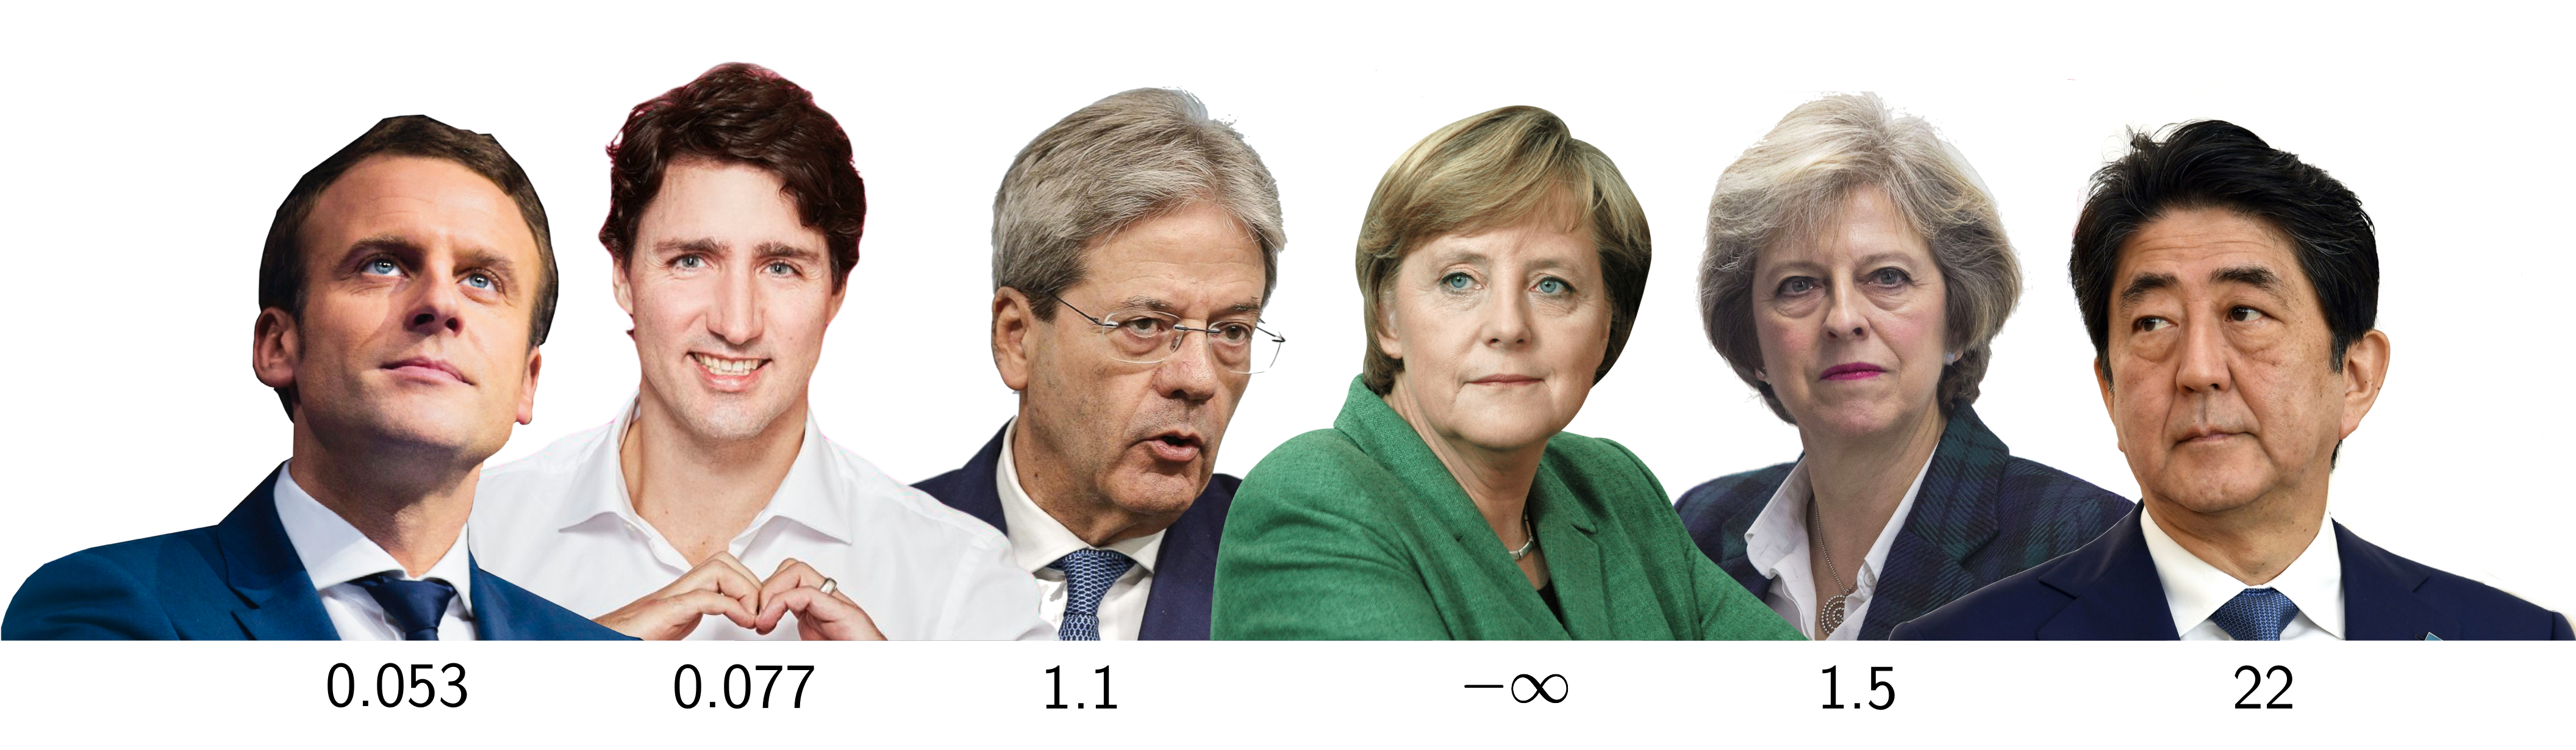
\includegraphics[width=12cm]{../../Graphics/G7Tweets.png}}

Assuming tweet wait times for heads of state arise from an exponential
distribution whose paramater is \(\lambda\):

\begin{itemize}
\tightlist
\item
  Write the total likelihood and log-likelihood function.
\item
  \beamerbutton{Advanced} Find the maximum likelihood estimate for
  \(\lambda\).
\item
  Plot the likelihood profile for \(\lambda\) using R.
\end{itemize}

\bigskip

\footnotetext[1]{Wait times between tweets collected with R package twitteR.}

\end{frame}

\begin{frame}{Likelihood and log likelihood functions and
\(\lambda_{MLE}\)\footnotemark}

\centerline{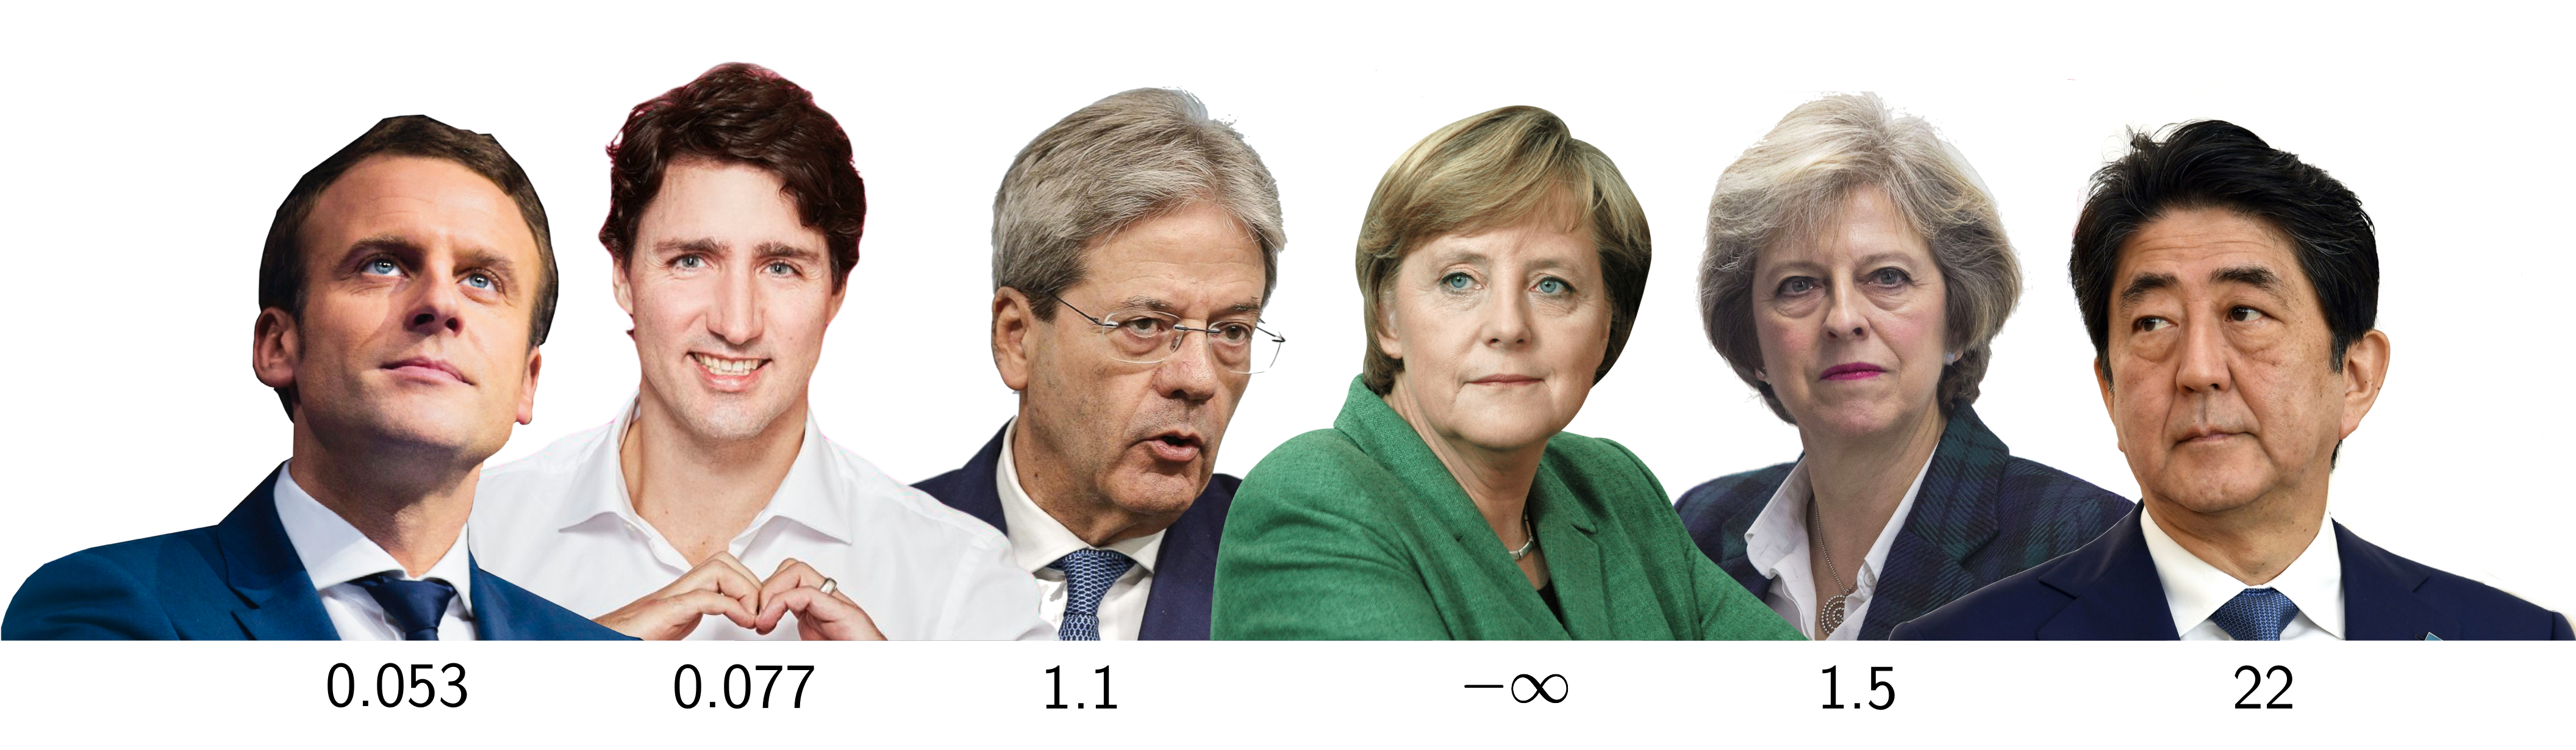
\includegraphics[width=12cm]{../../Graphics/G7Tweets.png}}

\vspace*{-1cm}

\begin{align*}
\mathscr{L}(\lambda) & = \prod_{i=1}^{6}[t_{i} \mid \lambda] & \frac{dL(\lambda)}{d\lambda}& = \frac{6}{\lambda}-\sum_{i=1}^{6}t_{i}\\
\Aboxed{\mathscr{L}(\lambda) & = \prod_{i=1}^{6}\lambda e^{-\lambda{t_{i}}}} & \lambda_{\textrm{MLE}} & =\frac{6}{24.9}= 0.24\\
\Aboxed{L(\lambda) & = 6\log(\lambda)-\lambda{(\sum_{i=1}^{6}t_{i})}} & \Aboxed{{\lambda_{\textrm{MLE}}} & =\frac{1}{\sum_{i=1}^{n}t_{i}/n}}
\end{align*}

\end{frame}

\begin{frame}[fragile]{Likelihood profile of \(\lambda\)}

\begin{center}
% Created by tikzDevice version 0.12 on 2019-08-01 22:58:23
% !TEX encoding = UTF-8 Unicode
\begin{tikzpicture}[x=1pt,y=1pt]
\definecolor{fillColor}{RGB}{255,255,255}
\begin{scope}
\definecolor{drawColor}{RGB}{0,0,255}

\path[draw=drawColor,line width= 0.8pt,line join=round,line cap=round] ( 57.15, 65.14) --
	( 57.35, 65.14) --
	( 57.55, 65.14) --
	( 57.75, 65.14) --
	( 57.95, 65.14) --
	( 58.15, 65.14) --
	( 58.34, 65.14) --
	( 58.54, 65.14) --
	( 58.74, 65.14) --
	( 58.94, 65.14) --
	( 59.14, 65.14) --
	( 59.34, 65.14) --
	( 59.54, 65.14) --
	( 59.74, 65.14) --
	( 59.94, 65.14) --
	( 60.14, 65.14) --
	( 60.33, 65.14) --
	( 60.53, 65.14) --
	( 60.73, 65.14) --
	( 60.93, 65.14) --
	( 61.13, 65.14) --
	( 61.33, 65.14) --
	( 61.53, 65.14) --
	( 61.73, 65.14) --
	( 61.93, 65.14) --
	( 62.13, 65.14) --
	( 62.32, 65.14) --
	( 62.52, 65.14) --
	( 62.72, 65.14) --
	( 62.92, 65.14) --
	( 63.12, 65.14) --
	( 63.32, 65.14) --
	( 63.52, 65.14) --
	( 63.72, 65.14) --
	( 63.92, 65.14) --
	( 64.12, 65.14) --
	( 64.31, 65.14) --
	( 64.51, 65.14) --
	( 64.71, 65.14) --
	( 64.91, 65.14) --
	( 65.11, 65.14) --
	( 65.31, 65.14) --
	( 65.51, 65.14) --
	( 65.71, 65.14) --
	( 65.91, 65.14) --
	( 66.11, 65.14) --
	( 66.30, 65.14) --
	( 66.50, 65.14) --
	( 66.70, 65.14) --
	( 66.90, 65.14) --
	( 67.10, 65.14) --
	( 67.30, 65.14) --
	( 67.50, 65.14) --
	( 67.70, 65.14) --
	( 67.90, 65.14) --
	( 68.09, 65.14) --
	( 68.29, 65.14) --
	( 68.49, 65.14) --
	( 68.69, 65.14) --
	( 68.89, 65.14) --
	( 69.09, 65.14) --
	( 69.29, 65.14) --
	( 69.49, 65.14) --
	( 69.69, 65.14) --
	( 69.89, 65.14) --
	( 70.08, 65.14) --
	( 70.28, 65.14) --
	( 70.48, 65.14) --
	( 70.68, 65.14) --
	( 70.88, 65.14) --
	( 71.08, 65.14) --
	( 71.28, 65.14) --
	( 71.48, 65.14) --
	( 71.68, 65.14) --
	( 71.88, 65.14) --
	( 72.07, 65.14) --
	( 72.27, 65.14) --
	( 72.47, 65.14) --
	( 72.67, 65.14) --
	( 72.87, 65.14) --
	( 73.07, 65.14) --
	( 73.27, 65.14) --
	( 73.47, 65.14) --
	( 73.67, 65.14) --
	( 73.87, 65.14) --
	( 74.06, 65.14) --
	( 74.26, 65.14) --
	( 74.46, 65.14) --
	( 74.66, 65.14) --
	( 74.86, 65.14) --
	( 75.06, 65.14) --
	( 75.26, 65.14) --
	( 75.46, 65.14) --
	( 75.66, 65.14) --
	( 75.85, 65.14) --
	( 76.05, 65.14) --
	( 76.25, 65.14) --
	( 76.45, 65.14) --
	( 76.65, 65.14) --
	( 76.85, 65.14) --
	( 77.05, 65.14) --
	( 77.25, 65.14) --
	( 77.45, 65.14) --
	( 77.65, 65.14) --
	( 77.84, 65.14) --
	( 78.04, 65.14) --
	( 78.24, 65.14) --
	( 78.44, 65.14) --
	( 78.64, 65.14) --
	( 78.84, 65.14) --
	( 79.04, 65.14) --
	( 79.24, 65.14) --
	( 79.44, 65.14) --
	( 79.64, 65.14) --
	( 79.83, 65.14) --
	( 80.03, 65.14) --
	( 80.23, 65.14) --
	( 80.43, 65.14) --
	( 80.63, 65.14) --
	( 80.83, 65.14) --
	( 81.03, 65.14) --
	( 81.23, 65.14) --
	( 81.43, 65.14) --
	( 81.63, 65.14) --
	( 81.82, 65.14) --
	( 82.02, 65.14) --
	( 82.22, 65.14) --
	( 82.42, 65.14) --
	( 82.62, 65.14) --
	( 82.82, 65.14) --
	( 83.02, 65.14) --
	( 83.22, 65.14) --
	( 83.42, 65.14) --
	( 83.62, 65.14) --
	( 83.81, 65.14) --
	( 84.01, 65.14) --
	( 84.21, 65.14) --
	( 84.41, 65.14) --
	( 84.61, 65.14) --
	( 84.81, 65.14) --
	( 85.01, 65.14) --
	( 85.21, 65.14) --
	( 85.41, 65.14) --
	( 85.60, 65.14) --
	( 85.80, 65.14) --
	( 86.00, 65.14) --
	( 86.20, 65.14) --
	( 86.40, 65.14) --
	( 86.60, 65.14) --
	( 86.80, 65.14) --
	( 87.00, 65.14) --
	( 87.20, 65.14) --
	( 87.40, 65.14) --
	( 87.59, 65.14) --
	( 87.79, 65.14) --
	( 87.99, 65.14) --
	( 88.19, 65.14) --
	( 88.39, 65.14) --
	( 88.59, 65.14) --
	( 88.79, 65.14) --
	( 88.99, 65.14) --
	( 89.19, 65.14) --
	( 89.39, 65.14) --
	( 89.58, 65.14) --
	( 89.78, 65.14) --
	( 89.98, 65.14) --
	( 90.18, 65.14) --
	( 90.38, 65.14) --
	( 90.58, 65.14) --
	( 90.78, 65.14) --
	( 90.98, 65.14) --
	( 91.18, 65.14) --
	( 91.38, 65.14) --
	( 91.57, 65.14) --
	( 91.77, 65.14) --
	( 91.97, 65.14) --
	( 92.17, 65.14) --
	( 92.37, 65.14) --
	( 92.57, 65.14) --
	( 92.77, 65.14) --
	( 92.97, 65.14) --
	( 93.17, 65.14) --
	( 93.36, 65.14) --
	( 93.56, 65.14) --
	( 93.76, 65.14) --
	( 93.96, 65.14) --
	( 94.16, 65.14) --
	( 94.36, 65.14) --
	( 94.56, 65.14) --
	( 94.76, 65.14) --
	( 94.96, 65.14) --
	( 95.16, 65.14) --
	( 95.35, 65.14) --
	( 95.55, 65.14) --
	( 95.75, 65.14) --
	( 95.95, 65.14) --
	( 96.15, 65.14) --
	( 96.35, 65.14) --
	( 96.55, 65.14) --
	( 96.75, 65.14) --
	( 96.95, 65.14) --
	( 97.15, 65.14) --
	( 97.34, 65.14) --
	( 97.54, 65.14) --
	( 97.74, 65.14) --
	( 97.94, 65.14) --
	( 98.14, 65.14) --
	( 98.34, 65.14) --
	( 98.54, 65.14) --
	( 98.74, 65.14) --
	( 98.94, 65.14) --
	( 99.14, 65.14) --
	( 99.33, 65.14) --
	( 99.53, 65.14) --
	( 99.73, 65.14) --
	( 99.93, 65.15) --
	(100.13, 65.15) --
	(100.33, 65.15) --
	(100.53, 65.15) --
	(100.73, 65.15) --
	(100.93, 65.15) --
	(101.12, 65.15) --
	(101.32, 65.15) --
	(101.52, 65.16) --
	(101.72, 65.16) --
	(101.92, 65.16) --
	(102.12, 65.16) --
	(102.32, 65.17) --
	(102.52, 65.17) --
	(102.72, 65.17) --
	(102.92, 65.18) --
	(103.11, 65.18) --
	(103.31, 65.19) --
	(103.51, 65.20) --
	(103.71, 65.21) --
	(103.91, 65.22) --
	(104.11, 65.23) --
	(104.31, 65.24) --
	(104.51, 65.25) --
	(104.71, 65.27) --
	(104.91, 65.28) --
	(105.10, 65.30) --
	(105.30, 65.32) --
	(105.50, 65.34) --
	(105.70, 65.37) --
	(105.90, 65.39) --
	(106.10, 65.43) --
	(106.30, 65.46) --
	(106.50, 65.50) --
	(106.70, 65.54) --
	(106.90, 65.58) --
	(107.09, 65.63) --
	(107.29, 65.69) --
	(107.49, 65.75) --
	(107.69, 65.81) --
	(107.89, 65.89) --
	(108.09, 65.97) --
	(108.29, 66.05) --
	(108.49, 66.14) --
	(108.69, 66.25) --
	(108.89, 66.36) --
	(109.08, 66.48) --
	(109.28, 66.61) --
	(109.48, 66.74) --
	(109.68, 66.90) --
	(109.88, 67.06) --
	(110.08, 67.23) --
	(110.28, 67.42) --
	(110.48, 67.62) --
	(110.68, 67.84) --
	(110.87, 68.07) --
	(111.07, 68.32) --
	(111.27, 68.59) --
	(111.47, 68.87) --
	(111.67, 69.17) --
	(111.87, 69.50) --
	(112.07, 69.84) --
	(112.27, 70.20) --
	(112.47, 70.58) --
	(112.67, 70.99) --
	(112.86, 71.42) --
	(113.06, 71.88) --
	(113.26, 72.36) --
	(113.46, 72.86) --
	(113.66, 73.39) --
	(113.86, 73.95) --
	(114.06, 74.54) --
	(114.26, 75.16) --
	(114.46, 75.80) --
	(114.66, 76.48) --
	(114.85, 77.18) --
	(115.05, 77.91) --
	(115.25, 78.68) --
	(115.45, 79.48) --
	(115.65, 80.31) --
	(115.85, 81.17) --
	(116.05, 82.06) --
	(116.25, 82.98) --
	(116.45, 83.94) --
	(116.65, 84.93) --
	(116.84, 85.94) --
	(117.04, 87.00) --
	(117.24, 88.08) --
	(117.44, 89.19) --
	(117.64, 90.33) --
	(117.84, 91.50) --
	(118.04, 92.71) --
	(118.24, 93.93) --
	(118.44, 95.19) --
	(118.63, 96.47) --
	(118.83, 97.78) --
	(119.03, 99.11) --
	(119.23,100.46) --
	(119.43,101.84) --
	(119.63,103.23) --
	(119.83,104.64) --
	(120.03,106.07) --
	(120.23,107.51) --
	(120.43,108.97) --
	(120.62,110.43) --
	(120.82,111.91) --
	(121.02,113.39) --
	(121.22,114.88) --
	(121.42,116.37) --
	(121.62,117.86) --
	(121.82,119.35) --
	(122.02,120.84) --
	(122.22,122.32) --
	(122.42,123.79) --
	(122.61,125.25) --
	(122.81,126.70) --
	(123.01,128.13) --
	(123.21,129.54) --
	(123.41,130.94) --
	(123.61,132.31) --
	(123.81,133.65) --
	(124.01,134.97) --
	(124.21,136.26) --
	(124.41,137.52) --
	(124.60,138.75) --
	(124.80,139.93) --
	(125.00,141.08) --
	(125.20,142.19) --
	(125.40,143.26) --
	(125.60,144.29) --
	(125.80,145.27) --
	(126.00,146.20) --
	(126.20,147.08) --
	(126.40,147.92) --
	(126.59,148.70) --
	(126.79,149.43) --
	(126.99,150.10) --
	(127.19,150.72) --
	(127.39,151.29) --
	(127.59,151.79) --
	(127.79,152.24) --
	(127.99,152.64) --
	(128.19,152.97) --
	(128.38,153.24) --
	(128.58,153.46) --
	(128.78,153.61) --
	(128.98,153.71) --
	(129.18,153.75) --
	(129.38,153.73) --
	(129.58,153.65) --
	(129.78,153.51) --
	(129.98,153.31) --
	(130.18,153.06) --
	(130.37,152.76) --
	(130.57,152.39) --
	(130.77,151.98) --
	(130.97,151.51) --
	(131.17,150.98) --
	(131.37,150.41) --
	(131.57,149.79) --
	(131.77,149.12) --
	(131.97,148.41) --
	(132.17,147.65) --
	(132.36,146.85) --
	(132.56,146.00) --
	(132.76,145.12) --
	(132.96,144.20) --
	(133.16,143.24) --
	(133.36,142.25) --
	(133.56,141.22) --
	(133.76,140.17) --
	(133.96,139.08) --
	(134.16,137.97) --
	(134.35,136.83) --
	(134.55,135.67) --
	(134.75,134.49) --
	(134.95,133.29) --
	(135.15,132.08) --
	(135.35,130.84) --
	(135.55,129.60) --
	(135.75,128.34) --
	(135.95,127.07) --
	(136.14,125.80) --
	(136.34,124.51) --
	(136.54,123.23) --
	(136.74,121.94) --
	(136.94,120.64) --
	(137.14,119.35) --
	(137.34,118.06) --
	(137.54,116.77) --
	(137.74,115.49) --
	(137.94,114.21) --
	(138.13,112.94) --
	(138.33,111.68) --
	(138.53,110.43) --
	(138.73,109.19) --
	(138.93,107.96) --
	(139.13,106.74) --
	(139.33,105.54) --
	(139.53,104.35) --
	(139.73,103.18) --
	(139.93,102.03) --
	(140.12,100.89) --
	(140.32, 99.77) --
	(140.52, 98.66) --
	(140.72, 97.58) --
	(140.92, 96.52) --
	(141.12, 95.47) --
	(141.32, 94.45) --
	(141.52, 93.45) --
	(141.72, 92.47) --
	(141.92, 91.51) --
	(142.11, 90.57) --
	(142.31, 89.65) --
	(142.51, 88.75) --
	(142.71, 87.88) --
	(142.91, 87.03) --
	(143.11, 86.20) --
	(143.31, 85.39) --
	(143.51, 84.61) --
	(143.71, 83.85) --
	(143.90, 83.10) --
	(144.10, 82.38) --
	(144.30, 81.68) --
	(144.50, 81.01) --
	(144.70, 80.35) --
	(144.90, 79.71) --
	(145.10, 79.10) --
	(145.30, 78.50) --
	(145.50, 77.93) --
	(145.70, 77.37) --
	(145.89, 76.83) --
	(146.09, 76.31) --
	(146.29, 75.81) --
	(146.49, 75.33) --
	(146.69, 74.86) --
	(146.89, 74.42) --
	(147.09, 73.99) --
	(147.29, 73.57) --
	(147.49, 73.17) --
	(147.69, 72.79) --
	(147.88, 72.42) --
	(148.08, 72.07) --
	(148.28, 71.73) --
	(148.48, 71.41) --
	(148.68, 71.10) --
	(148.88, 70.80) --
	(149.08, 70.51) --
	(149.28, 70.24) --
	(149.48, 69.98) --
	(149.68, 69.73) --
	(149.87, 69.49) --
	(150.07, 69.26) --
	(150.27, 69.05) --
	(150.47, 68.84) --
	(150.67, 68.64) --
	(150.87, 68.45) --
	(151.07, 68.27) --
	(151.27, 68.10) --
	(151.47, 67.94) --
	(151.67, 67.79) --
	(151.86, 67.64) --
	(152.06, 67.50) --
	(152.26, 67.37) --
	(152.46, 67.24) --
	(152.66, 67.12) --
	(152.86, 67.01) --
	(153.06, 66.90) --
	(153.26, 66.80) --
	(153.46, 66.70) --
	(153.65, 66.61) --
	(153.85, 66.52) --
	(154.05, 66.44) --
	(154.25, 66.36) --
	(154.45, 66.29) --
	(154.65, 66.22) --
	(154.85, 66.15) --
	(155.05, 66.09) --
	(155.25, 66.03) --
	(155.45, 65.98) --
	(155.64, 65.92) --
	(155.84, 65.88) --
	(156.04, 65.83) --
	(156.24, 65.79) --
	(156.44, 65.74) --
	(156.64, 65.71) --
	(156.84, 65.67) --
	(157.04, 65.64) --
	(157.24, 65.60) --
	(157.44, 65.57) --
	(157.63, 65.55) --
	(157.83, 65.52) --
	(158.03, 65.49) --
	(158.23, 65.47) --
	(158.43, 65.45) --
	(158.63, 65.43) --
	(158.83, 65.41) --
	(159.03, 65.39) --
	(159.23, 65.37) --
	(159.43, 65.36) --
	(159.62, 65.34) --
	(159.82, 65.33) --
	(160.02, 65.32) --
	(160.22, 65.30) --
	(160.42, 65.29) --
	(160.62, 65.28) --
	(160.82, 65.27) --
	(161.02, 65.26) --
	(161.22, 65.25) --
	(161.41, 65.25) --
	(161.61, 65.24) --
	(161.81, 65.23) --
	(162.01, 65.22) --
	(162.21, 65.22) --
	(162.41, 65.21) --
	(162.61, 65.21) --
	(162.81, 65.20) --
	(163.01, 65.20) --
	(163.21, 65.19) --
	(163.40, 65.19) --
	(163.60, 65.19) --
	(163.80, 65.18) --
	(164.00, 65.18) --
	(164.20, 65.18) --
	(164.40, 65.17) --
	(164.60, 65.17) --
	(164.80, 65.17) --
	(165.00, 65.17) --
	(165.20, 65.17) --
	(165.39, 65.16) --
	(165.59, 65.16) --
	(165.79, 65.16) --
	(165.99, 65.16) --
	(166.19, 65.16) --
	(166.39, 65.16) --
	(166.59, 65.15) --
	(166.79, 65.15) --
	(166.99, 65.15) --
	(167.19, 65.15) --
	(167.38, 65.15) --
	(167.58, 65.15) --
	(167.78, 65.15) --
	(167.98, 65.15) --
	(168.18, 65.15) --
	(168.38, 65.15) --
	(168.58, 65.15) --
	(168.78, 65.15) --
	(168.98, 65.15) --
	(169.18, 65.15) --
	(169.37, 65.15) --
	(169.57, 65.14) --
	(169.77, 65.14) --
	(169.97, 65.14) --
	(170.17, 65.14) --
	(170.37, 65.14) --
	(170.57, 65.14) --
	(170.77, 65.14) --
	(170.97, 65.14) --
	(171.16, 65.14) --
	(171.36, 65.14) --
	(171.56, 65.14) --
	(171.76, 65.14) --
	(171.96, 65.14) --
	(172.16, 65.14) --
	(172.36, 65.14) --
	(172.56, 65.14) --
	(172.76, 65.14) --
	(172.96, 65.14) --
	(173.15, 65.14) --
	(173.35, 65.14) --
	(173.55, 65.14) --
	(173.75, 65.14) --
	(173.95, 65.14) --
	(174.15, 65.14) --
	(174.35, 65.14) --
	(174.55, 65.14) --
	(174.75, 65.14) --
	(174.95, 65.14) --
	(175.14, 65.14) --
	(175.34, 65.14) --
	(175.54, 65.14) --
	(175.74, 65.14) --
	(175.94, 65.14) --
	(176.14, 65.14) --
	(176.34, 65.14) --
	(176.54, 65.14) --
	(176.74, 65.14) --
	(176.94, 65.14) --
	(177.13, 65.14) --
	(177.33, 65.14) --
	(177.53, 65.14) --
	(177.73, 65.14) --
	(177.93, 65.14) --
	(178.13, 65.14) --
	(178.33, 65.14) --
	(178.53, 65.14) --
	(178.73, 65.14) --
	(178.92, 65.14) --
	(179.12, 65.14) --
	(179.32, 65.14) --
	(179.52, 65.14) --
	(179.72, 65.14) --
	(179.92, 65.14) --
	(180.12, 65.14) --
	(180.32, 65.14) --
	(180.52, 65.14) --
	(180.72, 65.14) --
	(180.91, 65.14) --
	(181.11, 65.14) --
	(181.31, 65.14) --
	(181.51, 65.14) --
	(181.71, 65.14) --
	(181.91, 65.14) --
	(182.11, 65.14) --
	(182.31, 65.14) --
	(182.51, 65.14) --
	(182.71, 65.14) --
	(182.90, 65.14) --
	(183.10, 65.14) --
	(183.30, 65.14) --
	(183.50, 65.14) --
	(183.70, 65.14) --
	(183.90, 65.14) --
	(184.10, 65.14) --
	(184.30, 65.14) --
	(184.50, 65.14) --
	(184.70, 65.14) --
	(184.89, 65.14) --
	(185.09, 65.14) --
	(185.29, 65.14) --
	(185.49, 65.14) --
	(185.69, 65.14) --
	(185.89, 65.14) --
	(186.09, 65.14) --
	(186.29, 65.14) --
	(186.49, 65.14) --
	(186.68, 65.14) --
	(186.88, 65.14) --
	(187.08, 65.14) --
	(187.28, 65.14) --
	(187.48, 65.14) --
	(187.68, 65.14) --
	(187.88, 65.14) --
	(188.08, 65.14) --
	(188.28, 65.14) --
	(188.48, 65.14) --
	(188.67, 65.14) --
	(188.87, 65.14) --
	(189.07, 65.14) --
	(189.27, 65.14) --
	(189.47, 65.14) --
	(189.67, 65.14) --
	(189.87, 65.14) --
	(190.07, 65.14) --
	(190.27, 65.14) --
	(190.47, 65.14) --
	(190.66, 65.14) --
	(190.86, 65.14) --
	(191.06, 65.14) --
	(191.26, 65.14) --
	(191.46, 65.14) --
	(191.66, 65.14) --
	(191.86, 65.14) --
	(192.06, 65.14) --
	(192.26, 65.14) --
	(192.46, 65.14) --
	(192.65, 65.14) --
	(192.85, 65.14) --
	(193.05, 65.14) --
	(193.25, 65.14) --
	(193.45, 65.14) --
	(193.65, 65.14) --
	(193.85, 65.14) --
	(194.05, 65.14) --
	(194.25, 65.14) --
	(194.45, 65.14) --
	(194.64, 65.14) --
	(194.84, 65.14) --
	(195.04, 65.14) --
	(195.24, 65.14) --
	(195.44, 65.14) --
	(195.64, 65.14) --
	(195.84, 65.14) --
	(196.04, 65.14) --
	(196.24, 65.14) --
	(196.43, 65.14) --
	(196.63, 65.14) --
	(196.83, 65.14) --
	(197.03, 65.14) --
	(197.23, 65.14) --
	(197.43, 65.14) --
	(197.63, 65.14) --
	(197.83, 65.14) --
	(198.03, 65.14) --
	(198.23, 65.14) --
	(198.42, 65.14) --
	(198.62, 65.14) --
	(198.82, 65.14) --
	(199.02, 65.14) --
	(199.22, 65.14) --
	(199.42, 65.14) --
	(199.62, 65.14) --
	(199.82, 65.14) --
	(200.02, 65.14) --
	(200.22, 65.14) --
	(200.41, 65.14) --
	(200.61, 65.14) --
	(200.81, 65.14) --
	(201.01, 65.14) --
	(201.21, 65.14) --
	(201.41, 65.14) --
	(201.61, 65.14) --
	(201.81, 65.14) --
	(202.01, 65.14) --
	(202.21, 65.14) --
	(202.40, 65.14) --
	(202.60, 65.14) --
	(202.80, 65.14) --
	(203.00, 65.14) --
	(203.20, 65.14) --
	(203.40, 65.14) --
	(203.60, 65.14) --
	(203.80, 65.14) --
	(204.00, 65.14) --
	(204.19, 65.14) --
	(204.39, 65.14) --
	(204.59, 65.14) --
	(204.79, 65.14) --
	(204.99, 65.14) --
	(205.19, 65.14) --
	(205.39, 65.14) --
	(205.59, 65.14) --
	(205.79, 65.14) --
	(205.99, 65.14) --
	(206.18, 65.14) --
	(206.38, 65.14) --
	(206.58, 65.14) --
	(206.78, 65.14) --
	(206.98, 65.14) --
	(207.18, 65.14) --
	(207.38, 65.14) --
	(207.58, 65.14) --
	(207.78, 65.14) --
	(207.98, 65.14) --
	(208.17, 65.14) --
	(208.37, 65.14) --
	(208.57, 65.14) --
	(208.77, 65.14) --
	(208.97, 65.14) --
	(209.17, 65.14) --
	(209.37, 65.14) --
	(209.57, 65.14) --
	(209.77, 65.14) --
	(209.97, 65.14) --
	(210.16, 65.14) --
	(210.36, 65.14) --
	(210.56, 65.14) --
	(210.76, 65.14) --
	(210.96, 65.14) --
	(211.16, 65.14) --
	(211.36, 65.14) --
	(211.56, 65.14) --
	(211.76, 65.14) --
	(211.96, 65.14) --
	(212.15, 65.14) --
	(212.35, 65.14) --
	(212.55, 65.14) --
	(212.75, 65.14) --
	(212.95, 65.14) --
	(213.15, 65.14) --
	(213.35, 65.14) --
	(213.55, 65.14) --
	(213.75, 65.14) --
	(213.94, 65.14) --
	(214.14, 65.14) --
	(214.34, 65.14) --
	(214.54, 65.14) --
	(214.74, 65.14) --
	(214.94, 65.14) --
	(215.14, 65.14) --
	(215.34, 65.14) --
	(215.54, 65.14) --
	(215.74, 65.14) --
	(215.93, 65.14) --
	(216.13, 65.14) --
	(216.33, 65.14) --
	(216.53, 65.14) --
	(216.73, 65.14) --
	(216.93, 65.14) --
	(217.13, 65.14) --
	(217.33, 65.14) --
	(217.53, 65.14) --
	(217.73, 65.14) --
	(217.92, 65.14) --
	(218.12, 65.14) --
	(218.32, 65.14) --
	(218.52, 65.14) --
	(218.72, 65.14) --
	(218.92, 65.14) --
	(219.12, 65.14) --
	(219.32, 65.14) --
	(219.52, 65.14) --
	(219.72, 65.14) --
	(219.91, 65.14) --
	(220.11, 65.14) --
	(220.31, 65.14) --
	(220.51, 65.14) --
	(220.71, 65.14) --
	(220.91, 65.14) --
	(221.11, 65.14) --
	(221.31, 65.14) --
	(221.51, 65.14) --
	(221.70, 65.14) --
	(221.90, 65.14) --
	(222.10, 65.14) --
	(222.30, 65.14) --
	(222.50, 65.14) --
	(222.70, 65.14) --
	(222.90, 65.14) --
	(223.10, 65.14) --
	(223.30, 65.14) --
	(223.50, 65.14) --
	(223.69, 65.14) --
	(223.89, 65.14) --
	(224.09, 65.14) --
	(224.29, 65.14) --
	(224.49, 65.14) --
	(224.69, 65.14) --
	(224.89, 65.14) --
	(225.09, 65.14) --
	(225.29, 65.14) --
	(225.49, 65.14) --
	(225.68, 65.14) --
	(225.88, 65.14) --
	(226.08, 65.14) --
	(226.28, 65.14) --
	(226.48, 65.14) --
	(226.68, 65.14) --
	(226.88, 65.14) --
	(227.08, 65.14) --
	(227.28, 65.14) --
	(227.48, 65.14) --
	(227.67, 65.14) --
	(227.87, 65.14) --
	(228.07, 65.14) --
	(228.27, 65.14) --
	(228.47, 65.14) --
	(228.67, 65.14) --
	(228.87, 65.14) --
	(229.07, 65.14) --
	(229.27, 65.14) --
	(229.46, 65.14) --
	(229.66, 65.14) --
	(229.86, 65.14) --
	(230.06, 65.14) --
	(230.26, 65.14) --
	(230.46, 65.14) --
	(230.66, 65.14) --
	(230.86, 65.14) --
	(231.06, 65.14) --
	(231.26, 65.14) --
	(231.45, 65.14) --
	(231.65, 65.14) --
	(231.85, 65.14) --
	(232.05, 65.14) --
	(232.25, 65.14) --
	(232.45, 65.14) --
	(232.65, 65.14) --
	(232.85, 65.14) --
	(233.05, 65.14) --
	(233.25, 65.14) --
	(233.44, 65.14) --
	(233.64, 65.14) --
	(233.84, 65.14) --
	(234.04, 65.14) --
	(234.24, 65.14) --
	(234.44, 65.14) --
	(234.64, 65.14) --
	(234.84, 65.14) --
	(235.04, 65.14) --
	(235.24, 65.14) --
	(235.43, 65.14) --
	(235.63, 65.14) --
	(235.83, 65.14) --
	(236.03, 65.14) --
	(236.23, 65.14) --
	(236.43, 65.14) --
	(236.63, 65.14) --
	(236.83, 65.14) --
	(237.03, 65.14) --
	(237.23, 65.14) --
	(237.42, 65.14) --
	(237.62, 65.14) --
	(237.82, 65.14) --
	(238.02, 65.14) --
	(238.22, 65.14) --
	(238.42, 65.14) --
	(238.62, 65.14) --
	(238.82, 65.14) --
	(239.02, 65.14) --
	(239.21, 65.14) --
	(239.41, 65.14) --
	(239.61, 65.14) --
	(239.81, 65.14) --
	(240.01, 65.14) --
	(240.21, 65.14) --
	(240.41, 65.14) --
	(240.61, 65.14) --
	(240.81, 65.14) --
	(241.01, 65.14) --
	(241.20, 65.14) --
	(241.40, 65.14) --
	(241.60, 65.14) --
	(241.80, 65.14) --
	(242.00, 65.14) --
	(242.20, 65.14) --
	(242.40, 65.14) --
	(242.60, 65.14) --
	(242.80, 65.14) --
	(243.00, 65.14) --
	(243.19, 65.14) --
	(243.39, 65.14) --
	(243.59, 65.14) --
	(243.79, 65.14) --
	(243.99, 65.14) --
	(244.19, 65.14) --
	(244.39, 65.14) --
	(244.59, 65.14) --
	(244.79, 65.14) --
	(244.99, 65.14) --
	(245.18, 65.14) --
	(245.38, 65.14) --
	(245.58, 65.14) --
	(245.78, 65.14) --
	(245.98, 65.14) --
	(246.18, 65.14) --
	(246.38, 65.14) --
	(246.58, 65.14) --
	(246.78, 65.14) --
	(246.97, 65.14) --
	(247.17, 65.14) --
	(247.37, 65.14) --
	(247.57, 65.14) --
	(247.77, 65.14) --
	(247.97, 65.14) --
	(248.17, 65.14) --
	(248.37, 65.14) --
	(248.57, 65.14) --
	(248.77, 65.14) --
	(248.96, 65.14) --
	(249.16, 65.14) --
	(249.36, 65.14) --
	(249.56, 65.14) --
	(249.76, 65.14) --
	(249.96, 65.14) --
	(250.16, 65.14) --
	(250.36, 65.14) --
	(250.56, 65.14) --
	(250.76, 65.14) --
	(250.95, 65.14) --
	(251.15, 65.14) --
	(251.35, 65.14) --
	(251.55, 65.14) --
	(251.75, 65.14) --
	(251.95, 65.14) --
	(252.15, 65.14) --
	(252.35, 65.14) --
	(252.55, 65.14) --
	(252.75, 65.14) --
	(252.94, 65.14) --
	(253.14, 65.14) --
	(253.34, 65.14) --
	(253.54, 65.14) --
	(253.74, 65.14) --
	(253.94, 65.14) --
	(254.14, 65.14) --
	(254.34, 65.14) --
	(254.54, 65.14) --
	(254.74, 65.14) --
	(254.93, 65.14) --
	(255.13, 65.14) --
	(255.33, 65.14) --
	(255.53, 65.14) --
	(255.73, 65.14) --
	(255.93, 65.14);
\end{scope}
\begin{scope}
\definecolor{drawColor}{RGB}{0,0,0}

\path[draw=drawColor,line width= 0.4pt,line join=round,line cap=round] ( 49.20, 61.20) --
	(263.88, 61.20) --
	(263.88,167.61) --
	( 49.20,167.61) --
	( 49.20, 61.20);
\end{scope}
\begin{scope}
\definecolor{drawColor}{RGB}{0,0,0}

\path[draw=drawColor,line width= 0.4pt,line join=round,line cap=round] ( 57.15, 61.20) -- (255.93, 61.20);

\path[draw=drawColor,line width= 0.4pt,line join=round,line cap=round] ( 57.15, 61.20) -- ( 57.15, 55.20);

\path[draw=drawColor,line width= 0.4pt,line join=round,line cap=round] ( 82.00, 61.20) -- ( 82.00, 55.20);

\path[draw=drawColor,line width= 0.4pt,line join=round,line cap=round] (106.85, 61.20) -- (106.85, 55.20);

\path[draw=drawColor,line width= 0.4pt,line join=round,line cap=round] (131.69, 61.20) -- (131.69, 55.20);

\path[draw=drawColor,line width= 0.4pt,line join=round,line cap=round] (156.54, 61.20) -- (156.54, 55.20);

\path[draw=drawColor,line width= 0.4pt,line join=round,line cap=round] (181.39, 61.20) -- (181.39, 55.20);

\path[draw=drawColor,line width= 0.4pt,line join=round,line cap=round] (206.23, 61.20) -- (206.23, 55.20);

\path[draw=drawColor,line width= 0.4pt,line join=round,line cap=round] (231.08, 61.20) -- (231.08, 55.20);

\path[draw=drawColor,line width= 0.4pt,line join=round,line cap=round] (255.93, 61.20) -- (255.93, 55.20);

\node[text=drawColor,anchor=base,inner sep=0pt, outer sep=0pt, scale=  0.70] at ( 57.15, 39.60) {0};

\node[text=drawColor,anchor=base,inner sep=0pt, outer sep=0pt, scale=  0.70] at ( 82.00, 39.60) {5};

\node[text=drawColor,anchor=base,inner sep=0pt, outer sep=0pt, scale=  0.70] at (106.85, 39.60) {10};

\node[text=drawColor,anchor=base,inner sep=0pt, outer sep=0pt, scale=  0.70] at (131.69, 39.60) {15};

\node[text=drawColor,anchor=base,inner sep=0pt, outer sep=0pt, scale=  0.70] at (156.54, 39.60) {20};

\node[text=drawColor,anchor=base,inner sep=0pt, outer sep=0pt, scale=  0.70] at (181.39, 39.60) {25};

\node[text=drawColor,anchor=base,inner sep=0pt, outer sep=0pt, scale=  0.70] at (206.23, 39.60) {30};

\node[text=drawColor,anchor=base,inner sep=0pt, outer sep=0pt, scale=  0.70] at (231.08, 39.60) {35};

\node[text=drawColor,anchor=base,inner sep=0pt, outer sep=0pt, scale=  0.70] at (255.93, 39.60) {40};

\path[draw=drawColor,line width= 0.4pt,line join=round,line cap=round] ( 49.20, 65.14) -- ( 49.20,152.72);

\path[draw=drawColor,line width= 0.4pt,line join=round,line cap=round] ( 49.20, 65.14) -- ( 43.20, 65.14);

\path[draw=drawColor,line width= 0.4pt,line join=round,line cap=round] ( 49.20, 87.04) -- ( 43.20, 87.04);

\path[draw=drawColor,line width= 0.4pt,line join=round,line cap=round] ( 49.20,108.93) -- ( 43.20,108.93);

\path[draw=drawColor,line width= 0.4pt,line join=round,line cap=round] ( 49.20,130.83) -- ( 43.20,130.83);

\path[draw=drawColor,line width= 0.4pt,line join=round,line cap=round] ( 49.20,152.72) -- ( 43.20,152.72);

\node[text=drawColor,rotate= 90.00,anchor=base,inner sep=0pt, outer sep=0pt, scale=  0.50] at ( 34.80, 65.14) {0e+00};

\node[text=drawColor,rotate= 90.00,anchor=base,inner sep=0pt, outer sep=0pt, scale=  0.50] at ( 34.80, 87.04) {1e-29};

\node[text=drawColor,rotate= 90.00,anchor=base,inner sep=0pt, outer sep=0pt, scale=  0.50] at ( 34.80,108.93) {2e-29};

\node[text=drawColor,rotate= 90.00,anchor=base,inner sep=0pt, outer sep=0pt, scale=  0.50] at ( 34.80,130.83) {3e-29};

\node[text=drawColor,rotate= 90.00,anchor=base,inner sep=0pt, outer sep=0pt, scale=  0.50] at ( 34.80,152.72) {4e-29};

\node[text=drawColor,anchor=base,inner sep=0pt, outer sep=0pt, scale=  1.10] at (156.54, 21.60) {$\lambda$};

\node[text=drawColor,rotate= 90.00,anchor=base,inner sep=0pt, outer sep=0pt, scale=  1.10] at ( 16.80,114.41) {$\textnormal{L}(\lambda)$};
\end{scope}
\begin{scope}
\definecolor{fillColor}{RGB}{0,0,0}

\path[fill=fillColor] (129.18,153.75) circle (  2.81);
\end{scope}
\end{tikzpicture}

\end{center}

\tiny

\begin{Shaded}
\begin{Highlighting}[]
\NormalTok{lambda <-}\StringTok{ }\KeywordTok{seq}\NormalTok{(.}\DecValTok{01}\NormalTok{, }\DecValTok{1}\NormalTok{, }\DataTypeTok{length =} \DecValTok{1000}\NormalTok{)}
\NormalTok{y <-}\StringTok{ }\OtherTok{NA}
\ControlFlowTok{for}\NormalTok{(i }\ControlFlowTok{in} \DecValTok{1}\OperatorTok{:}\KeywordTok{length}\NormalTok{(lambda)) \{y[i] <-}\StringTok{ }\KeywordTok{prod}\NormalTok{(}\KeywordTok{dexp}\NormalTok{(}\KeywordTok{c}\NormalTok{(.}\DecValTok{15}\NormalTok{, }\FloatTok{1.5}\NormalTok{, }\DecValTok{22}\NormalTok{, .}\DecValTok{077}\NormalTok{, .}\DecValTok{0053}\NormalTok{, }\FloatTok{1.1}\NormalTok{), lambda[i]))\}}
\end{Highlighting}
\end{Shaded}

\end{frame}

\begin{frame}{Likelihood Surfaces}

\centerline{\includegraphics[width=9cm]{../../Graphics/LikelihoodSurface.png}}

\vspace*{1cm}

Figure courtesy of
\href{http://nesterko.com/lectures/stat221-2012/lecture8/\#/6}{\beamerbutton{Sergiy Nesterko}}.

\end{frame}

\begin{frame}{Main points}

\begin{itemize}
\tightlist
\item
  Likelihood allows us to evaluate the relative strength of evidence for
  one parameter or model relative to another.
\item
  The data are fixed and the parameters are variable in likelihood
  functions. These functions do not integrate or sum to one over the
  range of values of the parameter.
\item
  The data are variable and the parameter are fixed in probability mass
  functions and probability density functions. These functions sum or
  integrate to one over the support of the random variable, \(y\).
\end{itemize}

\end{frame}

\begin{frame}{Looking ahead: likelihood vs.~Bayes}

\begin{center}
% Created by tikzDevice version 0.12 on 2019-08-01 22:58:23
% !TEX encoding = UTF-8 Unicode
\begin{tikzpicture}[x=1pt,y=1pt]
\definecolor{fillColor}{RGB}{255,255,255}
\begin{scope}
\definecolor{drawColor}{RGB}{0,0,255}

\path[draw=drawColor,line width= 0.8pt,line join=round,line cap=round] ( 55.81, 63.80) --
	( 55.98, 63.80) --
	( 56.14, 63.80) --
	( 56.31, 63.80) --
	( 56.47, 63.80) --
	( 56.64, 63.80) --
	( 56.81, 63.80) --
	( 56.97, 63.80) --
	( 57.14, 63.80) --
	( 57.30, 63.80) --
	( 57.47, 63.80) --
	( 57.63, 63.80) --
	( 57.80, 63.80) --
	( 57.96, 63.80) --
	( 58.13, 63.80) --
	( 58.30, 63.81) --
	( 58.46, 63.81) --
	( 58.63, 63.81) --
	( 58.79, 63.81) --
	( 58.96, 63.81) --
	( 59.12, 63.81) --
	( 59.29, 63.81) --
	( 59.45, 63.81) --
	( 59.62, 63.82) --
	( 59.78, 63.82) --
	( 59.95, 63.82) --
	( 60.12, 63.82) --
	( 60.28, 63.83) --
	( 60.45, 63.83) --
	( 60.61, 63.84) --
	( 60.78, 63.84) --
	( 60.94, 63.84) --
	( 61.11, 63.85) --
	( 61.27, 63.86) --
	( 61.44, 63.86) --
	( 61.60, 63.87) --
	( 61.77, 63.88) --
	( 61.94, 63.88) --
	( 62.10, 63.89) --
	( 62.27, 63.90) --
	( 62.43, 63.91) --
	( 62.60, 63.92) --
	( 62.76, 63.93) --
	( 62.93, 63.95) --
	( 63.09, 63.96) --
	( 63.26, 63.97) --
	( 63.43, 63.99) --
	( 63.59, 64.00) --
	( 63.76, 64.02) --
	( 63.92, 64.04) --
	( 64.09, 64.05) --
	( 64.25, 64.07) --
	( 64.42, 64.09) --
	( 64.58, 64.11) --
	( 64.75, 64.14) --
	( 64.91, 64.16) --
	( 65.08, 64.18) --
	( 65.25, 64.21) --
	( 65.41, 64.24) --
	( 65.58, 64.26) --
	( 65.74, 64.29) --
	( 65.91, 64.32) --
	( 66.07, 64.35) --
	( 66.24, 64.39) --
	( 66.40, 64.42) --
	( 66.57, 64.46) --
	( 66.73, 64.49) --
	( 66.90, 64.53) --
	( 67.07, 64.57) --
	( 67.23, 64.61) --
	( 67.40, 64.65) --
	( 67.56, 64.70) --
	( 67.73, 64.74) --
	( 67.89, 64.79) --
	( 68.06, 64.84) --
	( 68.22, 64.89) --
	( 68.39, 64.94) --
	( 68.56, 64.99) --
	( 68.72, 65.05) --
	( 68.89, 65.11) --
	( 69.05, 65.17) --
	( 69.22, 65.23) --
	( 69.38, 65.29) --
	( 69.55, 65.35) --
	( 69.71, 65.42) --
	( 69.88, 65.48) --
	( 70.04, 65.55) --
	( 70.21, 65.62) --
	( 70.38, 65.70) --
	( 70.54, 65.77) --
	( 70.71, 65.85) --
	( 70.87, 65.92) --
	( 71.04, 66.00) --
	( 71.20, 66.09) --
	( 71.37, 66.17) --
	( 71.53, 66.26) --
	( 71.70, 66.34) --
	( 71.86, 66.44) --
	( 72.03, 66.53) --
	( 72.20, 66.62) --
	( 72.36, 66.72) --
	( 72.53, 66.82) --
	( 72.69, 66.92) --
	( 72.86, 67.02) --
	( 73.02, 67.12) --
	( 73.19, 67.23) --
	( 73.35, 67.34) --
	( 73.52, 67.45) --
	( 73.69, 67.56) --
	( 73.85, 67.68) --
	( 74.02, 67.79) --
	( 74.18, 67.91) --
	( 74.35, 68.03) --
	( 74.51, 68.16) --
	( 74.68, 68.28) --
	( 74.84, 68.41) --
	( 75.01, 68.54) --
	( 75.17, 68.67) --
	( 75.34, 68.81) --
	( 75.51, 68.94) --
	( 75.67, 69.08) --
	( 75.84, 69.22) --
	( 76.00, 69.37) --
	( 76.17, 69.51) --
	( 76.33, 69.66) --
	( 76.50, 69.81) --
	( 76.66, 69.96) --
	( 76.83, 70.12) --
	( 76.99, 70.27) --
	( 77.16, 70.43) --
	( 77.33, 70.59) --
	( 77.49, 70.76) --
	( 77.66, 70.92) --
	( 77.82, 71.09) --
	( 77.99, 71.26) --
	( 78.15, 71.43) --
	( 78.32, 71.61) --
	( 78.48, 71.78) --
	( 78.65, 71.96) --
	( 78.82, 72.14) --
	( 78.98, 72.32) --
	( 79.15, 72.51) --
	( 79.31, 72.70) --
	( 79.48, 72.88) --
	( 79.64, 73.08) --
	( 79.81, 73.27) --
	( 79.97, 73.47) --
	( 80.14, 73.66) --
	( 80.30, 73.86) --
	( 80.47, 74.07) --
	( 80.64, 74.27) --
	( 80.80, 74.48) --
	( 80.97, 74.68) --
	( 81.13, 74.89) --
	( 81.30, 75.11) --
	( 81.46, 75.32) --
	( 81.63, 75.54) --
	( 81.79, 75.76) --
	( 81.96, 75.98) --
	( 82.12, 76.20) --
	( 82.29, 76.42) --
	( 82.46, 76.65) --
	( 82.62, 76.88) --
	( 82.79, 77.11) --
	( 82.95, 77.34) --
	( 83.12, 77.57) --
	( 83.28, 77.81) --
	( 83.45, 78.05) --
	( 83.61, 78.29) --
	( 83.78, 78.53) --
	( 83.95, 78.77) --
	( 84.11, 79.01) --
	( 84.28, 79.26) --
	( 84.44, 79.51) --
	( 84.61, 79.76) --
	( 84.77, 80.01) --
	( 84.94, 80.26) --
	( 85.10, 80.52) --
	( 85.27, 80.78) --
	( 85.43, 81.03) --
	( 85.60, 81.29) --
	( 85.77, 81.55) --
	( 85.93, 81.82) --
	( 86.10, 82.08) --
	( 86.26, 82.35) --
	( 86.43, 82.61) --
	( 86.59, 82.88) --
	( 86.76, 83.15) --
	( 86.92, 83.43) --
	( 87.09, 83.70) --
	( 87.25, 83.97) --
	( 87.42, 84.25) --
	( 87.59, 84.53) --
	( 87.75, 84.80) --
	( 87.92, 85.08) --
	( 88.08, 85.36) --
	( 88.25, 85.65) --
	( 88.41, 85.93) --
	( 88.58, 86.21) --
	( 88.74, 86.50) --
	( 88.91, 86.79) --
	( 89.08, 87.07) --
	( 89.24, 87.36) --
	( 89.41, 87.65) --
	( 89.57, 87.94) --
	( 89.74, 88.23) --
	( 89.90, 88.53) --
	( 90.07, 88.82) --
	( 90.23, 89.11) --
	( 90.40, 89.41) --
	( 90.56, 89.71) --
	( 90.73, 90.00) --
	( 90.90, 90.30) --
	( 91.06, 90.60) --
	( 91.23, 90.90) --
	( 91.39, 91.20) --
	( 91.56, 91.50) --
	( 91.72, 91.80) --
	( 91.89, 92.10) --
	( 92.05, 92.40) --
	( 92.22, 92.70) --
	( 92.38, 93.01) --
	( 92.55, 93.31) --
	( 92.72, 93.61) --
	( 92.88, 93.92) --
	( 93.05, 94.22) --
	( 93.21, 94.53) --
	( 93.38, 94.83) --
	( 93.54, 95.14) --
	( 93.71, 95.45) --
	( 93.87, 95.75) --
	( 94.04, 96.06) --
	( 94.21, 96.37) --
	( 94.37, 96.67) --
	( 94.54, 96.98) --
	( 94.70, 97.29) --
	( 94.87, 97.59) --
	( 95.03, 97.90) --
	( 95.20, 98.21) --
	( 95.36, 98.51) --
	( 95.53, 98.82) --
	( 95.69, 99.13) --
	( 95.86, 99.43) --
	( 96.03, 99.74) --
	( 96.19,100.05) --
	( 96.36,100.35) --
	( 96.52,100.66) --
	( 96.69,100.96) --
	( 96.85,101.27) --
	( 97.02,101.57) --
	( 97.18,101.88) --
	( 97.35,102.18) --
	( 97.51,102.49) --
	( 97.68,102.79) --
	( 97.85,103.09) --
	( 98.01,103.39) --
	( 98.18,103.70) --
	( 98.34,104.00) --
	( 98.51,104.30) --
	( 98.67,104.60) --
	( 98.84,104.90) --
	( 99.00,105.19) --
	( 99.17,105.49) --
	( 99.34,105.79) --
	( 99.50,106.08) --
	( 99.67,106.38) --
	( 99.83,106.67) --
	(100.00,106.97) --
	(100.16,107.26) --
	(100.33,107.55) --
	(100.49,107.84) --
	(100.66,108.13) --
	(100.82,108.42) --
	(100.99,108.71) --
	(101.16,108.99) --
	(101.32,109.28) --
	(101.49,109.56) --
	(101.65,109.84) --
	(101.82,110.13) --
	(101.98,110.41) --
	(102.15,110.68) --
	(102.31,110.96) --
	(102.48,111.24) --
	(102.65,111.51) --
	(102.81,111.79) --
	(102.98,112.06) --
	(103.14,112.33) --
	(103.31,112.60) --
	(103.47,112.87) --
	(103.64,113.14) --
	(103.80,113.40) --
	(103.97,113.67) --
	(104.13,113.93) --
	(104.30,114.19) --
	(104.47,114.45) --
	(104.63,114.70) --
	(104.80,114.96) --
	(104.96,115.21) --
	(105.13,115.47) --
	(105.29,115.72) --
	(105.46,115.96) --
	(105.62,116.21) --
	(105.79,116.46) --
	(105.95,116.70) --
	(106.12,116.94) --
	(106.29,117.18) --
	(106.45,117.42) --
	(106.62,117.65) --
	(106.78,117.89) --
	(106.95,118.12) --
	(107.11,118.35) --
	(107.28,118.58) --
	(107.44,118.80) --
	(107.61,119.03) --
	(107.78,119.25) --
	(107.94,119.47) --
	(108.11,119.69) --
	(108.27,119.90) --
	(108.44,120.11) --
	(108.60,120.32) --
	(108.77,120.53) --
	(108.93,120.74) --
	(109.10,120.94) --
	(109.26,121.15) --
	(109.43,121.35) --
	(109.60,121.55) --
	(109.76,121.74) --
	(109.93,121.93) --
	(110.09,122.12) --
	(110.26,122.31) --
	(110.42,122.50) --
	(110.59,122.68) --
	(110.75,122.86) --
	(110.92,123.04) --
	(111.08,123.22) --
	(111.25,123.39) --
	(111.42,123.57) --
	(111.58,123.74) --
	(111.75,123.90) --
	(111.91,124.07) --
	(112.08,124.23) --
	(112.24,124.39) --
	(112.41,124.55) --
	(112.57,124.70) --
	(112.74,124.85) --
	(112.91,125.00) --
	(113.07,125.15) --
	(113.24,125.29) --
	(113.40,125.43) --
	(113.57,125.57) --
	(113.73,125.71) --
	(113.90,125.84) --
	(114.06,125.98) --
	(114.23,126.10) --
	(114.39,126.23) --
	(114.56,126.35) --
	(114.73,126.47) --
	(114.89,126.59) --
	(115.06,126.71) --
	(115.22,126.82) --
	(115.39,126.93) --
	(115.55,127.04) --
	(115.72,127.14) --
	(115.88,127.24) --
	(116.05,127.34) --
	(116.21,127.44) --
	(116.38,127.53) --
	(116.55,127.62) --
	(116.71,127.71) --
	(116.88,127.80) --
	(117.04,127.88) --
	(117.21,127.96) --
	(117.37,128.04) --
	(117.54,128.11) --
	(117.70,128.19) --
	(117.87,128.25) --
	(118.04,128.32) --
	(118.20,128.38) --
	(118.37,128.45) --
	(118.53,128.50) --
	(118.70,128.56) --
	(118.86,128.61) --
	(119.03,128.66) --
	(119.19,128.71) --
	(119.36,128.75) --
	(119.52,128.79) --
	(119.69,128.83) --
	(119.86,128.87) --
	(120.02,128.90) --
	(120.19,128.93) --
	(120.35,128.96) --
	(120.52,128.99) --
	(120.68,129.01) --
	(120.85,129.03) --
	(121.01,129.04) --
	(121.18,129.06) --
	(121.34,129.07) --
	(121.51,129.08) --
	(121.68,129.08) --
	(121.84,129.09) --
	(122.01,129.09) --
	(122.17,129.08) --
	(122.34,129.08) --
	(122.50,129.07) --
	(122.67,129.06) --
	(122.83,129.05) --
	(123.00,129.03) --
	(123.17,129.01) --
	(123.33,128.99) --
	(123.50,128.97) --
	(123.66,128.94) --
	(123.83,128.91) --
	(123.99,128.88) --
	(124.16,128.84) --
	(124.32,128.81) --
	(124.49,128.77) --
	(124.65,128.72) --
	(124.82,128.68) --
	(124.99,128.63) --
	(125.15,128.58) --
	(125.32,128.53) --
	(125.48,128.47) --
	(125.65,128.41) --
	(125.81,128.35) --
	(125.98,128.29) --
	(126.14,128.22) --
	(126.31,128.16) --
	(126.47,128.08) --
	(126.64,128.01) --
	(126.81,127.94) --
	(126.97,127.86) --
	(127.14,127.78) --
	(127.30,127.69) --
	(127.47,127.61) --
	(127.63,127.52) --
	(127.80,127.43) --
	(127.96,127.34) --
	(128.13,127.24) --
	(128.30,127.14) --
	(128.46,127.04) --
	(128.63,126.94) --
	(128.79,126.83) --
	(128.96,126.73) --
	(129.12,126.62) --
	(129.29,126.51) --
	(129.45,126.39) --
	(129.62,126.28) --
	(129.78,126.16) --
	(129.95,126.04) --
	(130.12,125.91) --
	(130.28,125.79) --
	(130.45,125.66) --
	(130.61,125.53) --
	(130.78,125.40) --
	(130.94,125.26) --
	(131.11,125.13) --
	(131.27,124.99) --
	(131.44,124.85) --
	(131.60,124.71) --
	(131.77,124.56) --
	(131.94,124.42) --
	(132.10,124.27) --
	(132.27,124.12) --
	(132.43,123.96) --
	(132.60,123.81) --
	(132.76,123.65) --
	(132.93,123.49) --
	(133.09,123.33) --
	(133.26,123.17) --
	(133.43,123.01) --
	(133.59,122.84) --
	(133.76,122.67) --
	(133.92,122.50) --
	(134.09,122.33) --
	(134.25,122.16) --
	(134.42,121.98) --
	(134.58,121.80) --
	(134.75,121.63) --
	(134.91,121.44) --
	(135.08,121.26) --
	(135.25,121.08) --
	(135.41,120.89) --
	(135.58,120.71) --
	(135.74,120.52) --
	(135.91,120.33) --
	(136.07,120.13) --
	(136.24,119.94) --
	(136.40,119.74) --
	(136.57,119.55) --
	(136.73,119.35) --
	(136.90,119.15) --
	(137.07,118.95) --
	(137.23,118.75) --
	(137.40,118.54) --
	(137.56,118.34) --
	(137.73,118.13) --
	(137.89,117.92) --
	(138.06,117.71) --
	(138.22,117.50) --
	(138.39,117.29) --
	(138.56,117.07) --
	(138.72,116.86) --
	(138.89,116.64) --
	(139.05,116.42) --
	(139.22,116.21) --
	(139.38,115.99) --
	(139.55,115.76) --
	(139.71,115.54) --
	(139.88,115.32) --
	(140.04,115.09) --
	(140.21,114.87) --
	(140.38,114.64) --
	(140.54,114.41) --
	(140.71,114.19) --
	(140.87,113.96) --
	(141.04,113.73) --
	(141.20,113.49) --
	(141.37,113.26) --
	(141.53,113.03) --
	(141.70,112.79) --
	(141.86,112.56) --
	(142.03,112.32) --
	(142.20,112.09) --
	(142.36,111.85) --
	(142.53,111.61) --
	(142.69,111.37) --
	(142.86,111.13) --
	(143.02,110.89) --
	(143.19,110.65) --
	(143.35,110.41) --
	(143.52,110.16) --
	(143.69,109.92) --
	(143.85,109.67) --
	(144.02,109.43) --
	(144.18,109.18) --
	(144.35,108.94) --
	(144.51,108.69) --
	(144.68,108.45) --
	(144.84,108.20) --
	(145.01,107.95) --
	(145.17,107.70) --
	(145.34,107.45) --
	(145.51,107.20) --
	(145.67,106.95) --
	(145.84,106.70) --
	(146.00,106.45) --
	(146.17,106.20) --
	(146.33,105.95) --
	(146.50,105.70) --
	(146.66,105.45) --
	(146.83,105.20) --
	(146.99,104.94) --
	(147.16,104.69) --
	(147.33,104.44) --
	(147.49,104.19) --
	(147.66,103.93) --
	(147.82,103.68) --
	(147.99,103.43) --
	(148.15,103.17) --
	(148.32,102.92) --
	(148.48,102.67) --
	(148.65,102.41) --
	(148.82,102.16) --
	(148.98,101.91) --
	(149.15,101.65) --
	(149.31,101.40) --
	(149.48,101.14) --
	(149.64,100.89) --
	(149.81,100.64) --
	(149.97,100.38) --
	(150.14,100.13) --
	(150.30, 99.88) --
	(150.47, 99.63) --
	(150.64, 99.37) --
	(150.80, 99.12) --
	(150.97, 98.87) --
	(151.13, 98.62) --
	(151.30, 98.36) --
	(151.46, 98.11) --
	(151.63, 97.86) --
	(151.79, 97.61) --
	(151.96, 97.36) --
	(152.13, 97.11) --
	(152.29, 96.86) --
	(152.46, 96.61) --
	(152.62, 96.36) --
	(152.79, 96.11) --
	(152.95, 95.86) --
	(153.12, 95.61) --
	(153.28, 95.36) --
	(153.45, 95.12) --
	(153.61, 94.87) --
	(153.78, 94.62) --
	(153.95, 94.38) --
	(154.11, 94.13) --
	(154.28, 93.89) --
	(154.44, 93.64) --
	(154.61, 93.40) --
	(154.77, 93.16) --
	(154.94, 92.91) --
	(155.10, 92.67) --
	(155.27, 92.43) --
	(155.43, 92.19) --
	(155.60, 91.95) --
	(155.77, 91.71) --
	(155.93, 91.47) --
	(156.10, 91.23) --
	(156.26, 91.00) --
	(156.43, 90.76) --
	(156.59, 90.52) --
	(156.76, 90.29) --
	(156.92, 90.05) --
	(157.09, 89.82) --
	(157.26, 89.59) --
	(157.42, 89.36) --
	(157.59, 89.12) --
	(157.75, 88.89) --
	(157.92, 88.66) --
	(158.08, 88.44) --
	(158.25, 88.21) --
	(158.41, 87.98) --
	(158.58, 87.75) --
	(158.74, 87.53) --
	(158.91, 87.30) --
	(159.08, 87.08) --
	(159.24, 86.86) --
	(159.41, 86.64) --
	(159.57, 86.41) --
	(159.74, 86.19) --
	(159.90, 85.98) --
	(160.07, 85.76) --
	(160.23, 85.54) --
	(160.40, 85.32) --
	(160.56, 85.11) --
	(160.73, 84.89) --
	(160.90, 84.68) --
	(161.06, 84.47) --
	(161.23, 84.26) --
	(161.39, 84.05) --
	(161.56, 83.84) --
	(161.72, 83.63) --
	(161.89, 83.42) --
	(162.05, 83.22) --
	(162.22, 83.01) --
	(162.39, 82.81) --
	(162.55, 82.61) --
	(162.72, 82.41) --
	(162.88, 82.21) --
	(163.05, 82.01) --
	(163.21, 81.81) --
	(163.38, 81.61) --
	(163.54, 81.41) --
	(163.71, 81.22) --
	(163.87, 81.03) --
	(164.04, 80.83) --
	(164.21, 80.64) --
	(164.37, 80.45) --
	(164.54, 80.26) --
	(164.70, 80.07) --
	(164.87, 79.89) --
	(165.03, 79.70) --
	(165.20, 79.52) --
	(165.36, 79.33) --
	(165.53, 79.15) --
	(165.69, 78.97) --
	(165.86, 78.79) --
	(166.03, 78.61) --
	(166.19, 78.44) --
	(166.36, 78.26) --
	(166.52, 78.08) --
	(166.69, 77.91) --
	(166.85, 77.74) --
	(167.02, 77.57) --
	(167.18, 77.40) --
	(167.35, 77.23) --
	(167.52, 77.06) --
	(167.68, 76.89) --
	(167.85, 76.73) --
	(168.01, 76.57) --
	(168.18, 76.40) --
	(168.34, 76.24) --
	(168.51, 76.08) --
	(168.67, 75.92) --
	(168.84, 75.76) --
	(169.00, 75.61) --
	(169.17, 75.45) --
	(169.34, 75.30) --
	(169.50, 75.15) --
	(169.67, 75.00) --
	(169.83, 74.84) --
	(170.00, 74.70) --
	(170.16, 74.55) --
	(170.33, 74.40) --
	(170.49, 74.26) --
	(170.66, 74.11) --
	(170.82, 73.97) --
	(170.99, 73.83) --
	(171.16, 73.69) --
	(171.32, 73.55) --
	(171.49, 73.41) --
	(171.65, 73.27) --
	(171.82, 73.14) --
	(171.98, 73.00) --
	(172.15, 72.87) --
	(172.31, 72.74) --
	(172.48, 72.61) --
	(172.65, 72.48) --
	(172.81, 72.35) --
	(172.98, 72.23) --
	(173.14, 72.10) --
	(173.31, 71.98) --
	(173.47, 71.85) --
	(173.64, 71.73) --
	(173.80, 71.61) --
	(173.97, 71.49) --
	(174.13, 71.37) --
	(174.30, 71.26) --
	(174.47, 71.14) --
	(174.63, 71.03) --
	(174.80, 70.91) --
	(174.96, 70.80) --
	(175.13, 70.69) --
	(175.29, 70.58) --
	(175.46, 70.47) --
	(175.62, 70.36) --
	(175.79, 70.26) --
	(175.95, 70.15) --
	(176.12, 70.05) --
	(176.29, 69.95) --
	(176.45, 69.84) --
	(176.62, 69.74) --
	(176.78, 69.64) --
	(176.95, 69.55) --
	(177.11, 69.45) --
	(177.28, 69.35) --
	(177.44, 69.26) --
	(177.61, 69.16) --
	(177.78, 69.07) --
	(177.94, 68.98) --
	(178.11, 68.89) --
	(178.27, 68.80) --
	(178.44, 68.71) --
	(178.60, 68.62) --
	(178.77, 68.54) --
	(178.93, 68.45) --
	(179.10, 68.37) --
	(179.26, 68.29) --
	(179.43, 68.21) --
	(179.60, 68.12) --
	(179.76, 68.04) --
	(179.93, 67.97) --
	(180.09, 67.89) --
	(180.26, 67.81) --
	(180.42, 67.74) --
	(180.59, 67.66) --
	(180.75, 67.59) --
	(180.92, 67.52) --
	(181.08, 67.44) --
	(181.25, 67.37) --
	(181.42, 67.30) --
	(181.58, 67.24) --
	(181.75, 67.17) --
	(181.91, 67.10) --
	(182.08, 67.04) --
	(182.24, 66.97) --
	(182.41, 66.91) --
	(182.57, 66.84) --
	(182.74, 66.78) --
	(182.91, 66.72) --
	(183.07, 66.66) --
	(183.24, 66.60) --
	(183.40, 66.54) --
	(183.57, 66.49) --
	(183.73, 66.43) --
	(183.90, 66.37) --
	(184.06, 66.32) --
	(184.23, 66.26) --
	(184.39, 66.21) --
	(184.56, 66.16) --
	(184.73, 66.11) --
	(184.89, 66.06) --
	(185.06, 66.01) --
	(185.22, 65.96) --
	(185.39, 65.91) --
	(185.55, 65.86) --
	(185.72, 65.82) --
	(185.88, 65.77) --
	(186.05, 65.73) --
	(186.21, 65.68) --
	(186.38, 65.64) --
	(186.55, 65.59) --
	(186.71, 65.55) --
	(186.88, 65.51) --
	(187.04, 65.47) --
	(187.21, 65.43) --
	(187.37, 65.39) --
	(187.54, 65.35) --
	(187.70, 65.32) --
	(187.87, 65.28) --
	(188.04, 65.24) --
	(188.20, 65.21) --
	(188.37, 65.17) --
	(188.53, 65.14) --
	(188.70, 65.10) --
	(188.86, 65.07) --
	(189.03, 65.04) --
	(189.19, 65.01) --
	(189.36, 64.98) --
	(189.52, 64.95) --
	(189.69, 64.92) --
	(189.86, 64.89) --
	(190.02, 64.86) --
	(190.19, 64.83) --
	(190.35, 64.80) --
	(190.52, 64.77) --
	(190.68, 64.75) --
	(190.85, 64.72) --
	(191.01, 64.70) --
	(191.18, 64.67) --
	(191.34, 64.65) --
	(191.51, 64.62) --
	(191.68, 64.60) --
	(191.84, 64.58) --
	(192.01, 64.56) --
	(192.17, 64.53) --
	(192.34, 64.51) --
	(192.50, 64.49) --
	(192.67, 64.47) --
	(192.83, 64.45) --
	(193.00, 64.43) --
	(193.17, 64.41) --
	(193.33, 64.39) --
	(193.50, 64.38) --
	(193.66, 64.36) --
	(193.83, 64.34) --
	(193.99, 64.32) --
	(194.16, 64.31) --
	(194.32, 64.29) --
	(194.49, 64.28) --
	(194.65, 64.26) --
	(194.82, 64.25) --
	(194.99, 64.23) --
	(195.15, 64.22) --
	(195.32, 64.20) --
	(195.48, 64.19) --
	(195.65, 64.18) --
	(195.81, 64.17) --
	(195.98, 64.15) --
	(196.14, 64.14) --
	(196.31, 64.13) --
	(196.47, 64.12) --
	(196.64, 64.11) --
	(196.81, 64.10) --
	(196.97, 64.09) --
	(197.14, 64.08) --
	(197.30, 64.07) --
	(197.47, 64.06) --
	(197.63, 64.05) --
	(197.80, 64.04) --
	(197.96, 64.03) --
	(198.13, 64.02) --
	(198.30, 64.01) --
	(198.46, 64.00) --
	(198.63, 64.00) --
	(198.79, 63.99) --
	(198.96, 63.98) --
	(199.12, 63.97) --
	(199.29, 63.97) --
	(199.45, 63.96) --
	(199.62, 63.95) --
	(199.78, 63.95) --
	(199.95, 63.94) --
	(200.12, 63.94) --
	(200.28, 63.93) --
	(200.45, 63.93) --
	(200.61, 63.92) --
	(200.78, 63.92) --
	(200.94, 63.91) --
	(201.11, 63.91) --
	(201.27, 63.90) --
	(201.44, 63.90) --
	(201.61, 63.89) --
	(201.77, 63.89) --
	(201.94, 63.88) --
	(202.10, 63.88) --
	(202.27, 63.88) --
	(202.43, 63.87) --
	(202.60, 63.87) --
	(202.76, 63.87) --
	(202.93, 63.86) --
	(203.09, 63.86) --
	(203.26, 63.86) --
	(203.43, 63.86) --
	(203.59, 63.85) --
	(203.76, 63.85) --
	(203.92, 63.85) --
	(204.09, 63.85) --
	(204.25, 63.84) --
	(204.42, 63.84) --
	(204.58, 63.84) --
	(204.75, 63.84) --
	(204.91, 63.84) --
	(205.08, 63.83) --
	(205.25, 63.83) --
	(205.41, 63.83) --
	(205.58, 63.83) --
	(205.74, 63.83) --
	(205.91, 63.83) --
	(206.07, 63.82) --
	(206.24, 63.82) --
	(206.40, 63.82) --
	(206.57, 63.82) --
	(206.74, 63.82) --
	(206.90, 63.82) --
	(207.07, 63.82) --
	(207.23, 63.82) --
	(207.40, 63.82) --
	(207.56, 63.81) --
	(207.73, 63.81) --
	(207.89, 63.81) --
	(208.06, 63.81) --
	(208.22, 63.81) --
	(208.39, 63.81) --
	(208.56, 63.81) --
	(208.72, 63.81) --
	(208.89, 63.81) --
	(209.05, 63.81) --
	(209.22, 63.81) --
	(209.38, 63.81) --
	(209.55, 63.81) --
	(209.71, 63.81) --
	(209.88, 63.81) --
	(210.04, 63.81) --
	(210.21, 63.81) --
	(210.38, 63.81) --
	(210.54, 63.81) --
	(210.71, 63.81) --
	(210.87, 63.81) --
	(211.04, 63.80) --
	(211.20, 63.80) --
	(211.37, 63.80) --
	(211.53, 63.80) --
	(211.70, 63.80) --
	(211.87, 63.80) --
	(212.03, 63.80) --
	(212.20, 63.80) --
	(212.36, 63.80) --
	(212.53, 63.80) --
	(212.69, 63.80) --
	(212.86, 63.80) --
	(213.02, 63.80) --
	(213.19, 63.80) --
	(213.35, 63.80) --
	(213.52, 63.80) --
	(213.69, 63.80) --
	(213.85, 63.80) --
	(214.02, 63.80) --
	(214.18, 63.80) --
	(214.35, 63.80) --
	(214.51, 63.80) --
	(214.68, 63.80) --
	(214.84, 63.80) --
	(215.01, 63.80) --
	(215.17, 63.80) --
	(215.34, 63.80) --
	(215.51, 63.80) --
	(215.67, 63.80) --
	(215.84, 63.80) --
	(216.00, 63.80) --
	(216.17, 63.80) --
	(216.33, 63.80) --
	(216.50, 63.80) --
	(216.66, 63.80) --
	(216.83, 63.80) --
	(217.00, 63.80) --
	(217.16, 63.80) --
	(217.33, 63.80) --
	(217.49, 63.80) --
	(217.66, 63.80) --
	(217.82, 63.80) --
	(217.99, 63.80) --
	(218.15, 63.80) --
	(218.32, 63.80) --
	(218.48, 63.80) --
	(218.65, 63.80) --
	(218.82, 63.80) --
	(218.98, 63.80) --
	(219.15, 63.80) --
	(219.31, 63.80) --
	(219.48, 63.80) --
	(219.64, 63.80) --
	(219.81, 63.80) --
	(219.97, 63.80) --
	(220.14, 63.80) --
	(220.30, 63.80) --
	(220.47, 63.80) --
	(220.64, 63.80) --
	(220.80, 63.80) --
	(220.97, 63.80) --
	(221.13, 63.80);
\end{scope}
\begin{scope}
\definecolor{drawColor}{RGB}{0,0,0}

\path[draw=drawColor,line width= 0.4pt,line join=round,line cap=round] ( 49.20, 61.20) --
	(227.75, 61.20) --
	(227.75,131.47) --
	( 49.20,131.47) --
	( 49.20, 61.20);
\end{scope}
\begin{scope}
\definecolor{drawColor}{RGB}{0,0,0}

\path[draw=drawColor,line width= 0.4pt,line join=round,line cap=round] ( 55.81, 61.20) -- (221.13, 61.20);

\path[draw=drawColor,line width= 0.4pt,line join=round,line cap=round] ( 55.81, 61.20) -- ( 55.81, 55.20);

\path[draw=drawColor,line width= 0.4pt,line join=round,line cap=round] ( 88.88, 61.20) -- ( 88.88, 55.20);

\path[draw=drawColor,line width= 0.4pt,line join=round,line cap=round] (121.94, 61.20) -- (121.94, 55.20);

\path[draw=drawColor,line width= 0.4pt,line join=round,line cap=round] (155.00, 61.20) -- (155.00, 55.20);

\path[draw=drawColor,line width= 0.4pt,line join=round,line cap=round] (188.07, 61.20) -- (188.07, 55.20);

\path[draw=drawColor,line width= 0.4pt,line join=round,line cap=round] (221.13, 61.20) -- (221.13, 55.20);

\node[text=drawColor,anchor=base,inner sep=0pt, outer sep=0pt, scale=  0.70] at ( 55.81, 39.60) {0.0};

\node[text=drawColor,anchor=base,inner sep=0pt, outer sep=0pt, scale=  0.70] at ( 88.88, 39.60) {0.2};

\node[text=drawColor,anchor=base,inner sep=0pt, outer sep=0pt, scale=  0.70] at (121.94, 39.60) {0.4};

\node[text=drawColor,anchor=base,inner sep=0pt, outer sep=0pt, scale=  0.70] at (155.00, 39.60) {0.6};

\node[text=drawColor,anchor=base,inner sep=0pt, outer sep=0pt, scale=  0.70] at (188.07, 39.60) {0.8};

\node[text=drawColor,anchor=base,inner sep=0pt, outer sep=0pt, scale=  0.70] at (221.13, 39.60) {1.0};

\path[draw=drawColor,line width= 0.4pt,line join=round,line cap=round] ( 49.20, 63.80) -- ( 49.20,128.87);

\path[draw=drawColor,line width= 0.4pt,line join=round,line cap=round] ( 49.20, 63.80) -- ( 43.20, 63.80);

\path[draw=drawColor,line width= 0.4pt,line join=round,line cap=round] ( 49.20, 76.82) -- ( 43.20, 76.82);

\path[draw=drawColor,line width= 0.4pt,line join=round,line cap=round] ( 49.20, 89.83) -- ( 43.20, 89.83);

\path[draw=drawColor,line width= 0.4pt,line join=round,line cap=round] ( 49.20,102.84) -- ( 43.20,102.84);

\path[draw=drawColor,line width= 0.4pt,line join=round,line cap=round] ( 49.20,115.86) -- ( 43.20,115.86);

\path[draw=drawColor,line width= 0.4pt,line join=round,line cap=round] ( 49.20,128.87) -- ( 43.20,128.87);

\node[text=drawColor,rotate= 90.00,anchor=base,inner sep=0pt, outer sep=0pt, scale=  0.50] at ( 34.80, 63.80) {0.00};

\node[text=drawColor,rotate= 90.00,anchor=base,inner sep=0pt, outer sep=0pt, scale=  0.50] at ( 34.80, 89.83) {0.10};

\node[text=drawColor,rotate= 90.00,anchor=base,inner sep=0pt, outer sep=0pt, scale=  0.50] at ( 34.80,115.86) {0.20};

\node[text=drawColor,anchor=base,inner sep=0pt, outer sep=0pt, scale=  1.10] at (138.47, 27.60) {$\theta$};

\node[text=drawColor,rotate= 90.00,anchor=base,inner sep=0pt, outer sep=0pt, scale=  1.10] at ( 22.80, 96.34) {$\textnormal{L}(\theta)$};
\end{scope}
\end{tikzpicture}

\end{center}

\begin{itemize}
\tightlist
\item
  What must be done to insure that the area under the curve = 1?
\item
  If you do this, is this now a probability density function for
  \(\theta\)?
\end{itemize}

\end{frame}

\begin{frame}{Likelihood ratio confidence intervals}

Find the upper and lower bounds of an interval where all \(\lambda\)
values within that interval are as consistent with the data as
\(\lambda_{MLE}\).

We compute the likelihood ratio statistic:

\[\mathscr{R} = 2\log\Big(\frac{\mathscr{L}(\lambda_{MLE} \mid t_{1})}{\mathscr{L}(\lambda_{0}\mid t_{1})}\Big)  \sim \chi_{k=1}^{2}\]

which is distributed \(\chi^{2}\) with 1 degree of freedom. Note that we
fail to reject \(H_{0}\) that \(\lambda = \lambda_{0}\) if
\(\mathscr{R} < \chi_{k=1}^{2}(1 - \alpha)\).

\end{frame}

\begin{frame}{Likelihood ratio confidence intervals}

We determine the \((1-\alpha = 0.95)\) likelihood ratio confidence
interval by finding the upper and lower bounds for all values of
\(\lambda_{0}\) where we would fail to reject \(H_{0}\).

\begin{eqnarray*}
2\log\Big(\frac{\mathscr{L}(\lambda_{MLE} \mid t_{1})}{\mathscr{L}(\lambda\mid t_{1})}\Big) < \chi_{k=1}^{2}(0.95)\\
L(\lambda_{MLE}) - \frac{3.84}{2} < L(\lambda\mid t_{1})\\
L(\lambda\mid t_{1}) > L(\lambda_{MLE}) - 1.92
\end{eqnarray*}

\end{frame}

\begin{frame}{Likelihood ratio confidence intervals}

\begin{center}
% Created by tikzDevice version 0.12 on 2019-05-05 19:34:47
% !TEX encoding = UTF-8 Unicode
\begin{tikzpicture}[x=1pt,y=1pt]
\definecolor{fillColor}{RGB}{255,255,255}
\begin{scope}
\definecolor{drawColor}{RGB}{0,0,255}

\path[draw=drawColor,line width= 0.8pt,line join=round,line cap=round] ( 57.82, 75.20) --
	( 58.04, 88.43) --
	( 58.25, 96.13) --
	( 58.47,101.57) --
	( 58.68,105.77) --
	( 58.90,109.19) --
	( 59.11,112.06) --
	( 59.33,114.54) --
	( 59.55,116.72) --
	( 59.76,118.66) --
	( 59.98,120.40) --
	( 60.19,121.99) --
	( 60.41,123.44) --
	( 60.62,124.77) --
	( 60.84,126.01) --
	( 61.06,127.17) --
	( 61.27,128.24) --
	( 61.49,129.26) --
	( 61.70,130.21) --
	( 61.92,131.11) --
	( 62.13,131.96) --
	( 62.35,132.76) --
	( 62.57,133.53) --
	( 62.78,134.26) --
	( 63.00,134.96) --
	( 63.21,135.63) --
	( 63.43,136.27) --
	( 63.64,136.88) --
	( 63.86,137.47) --
	( 64.08,138.03) --
	( 64.29,138.57) --
	( 64.51,139.10) --
	( 64.72,139.60) --
	( 64.94,140.09) --
	( 65.15,140.56) --
	( 65.37,141.01) --
	( 65.59,141.45) --
	( 65.80,141.88) --
	( 66.02,142.29) --
	( 66.23,142.69) --
	( 66.45,143.08) --
	( 66.66,143.46) --
	( 66.88,143.82) --
	( 67.10,144.18) --
	( 67.31,144.52) --
	( 67.53,144.86) --
	( 67.74,145.19) --
	( 67.96,145.50) --
	( 68.17,145.81) --
	( 68.39,146.11) --
	( 68.61,146.41) --
	( 68.82,146.70) --
	( 69.04,146.97) --
	( 69.25,147.25) --
	( 69.47,147.51) --
	( 69.69,147.77) --
	( 69.90,148.03) --
	( 70.12,148.27) --
	( 70.33,148.52) --
	( 70.55,148.75) --
	( 70.76,148.98) --
	( 70.98,149.21) --
	( 71.20,149.43) --
	( 71.41,149.65) --
	( 71.63,149.86) --
	( 71.84,150.06) --
	( 72.06,150.27) --
	( 72.27,150.47) --
	( 72.49,150.66) --
	( 72.71,150.85) --
	( 72.92,151.04) --
	( 73.14,151.22) --
	( 73.35,151.40) --
	( 73.57,151.57) --
	( 73.78,151.74) --
	( 74.00,151.91) --
	( 74.22,152.08) --
	( 74.43,152.24) --
	( 74.65,152.39) --
	( 74.86,152.55) --
	( 75.08,152.70) --
	( 75.29,152.85) --
	( 75.51,153.00) --
	( 75.73,153.14) --
	( 75.94,153.28) --
	( 76.16,153.42) --
	( 76.37,153.56) --
	( 76.59,153.69) --
	( 76.80,153.82) --
	( 77.02,153.95) --
	( 77.24,154.07) --
	( 77.45,154.20) --
	( 77.67,154.32) --
	( 77.88,154.44) --
	( 78.10,154.55) --
	( 78.31,154.67) --
	( 78.53,154.78) --
	( 78.75,154.89) --
	( 78.96,155.00) --
	( 79.18,155.11) --
	( 79.39,155.21) --
	( 79.61,155.32) --
	( 79.82,155.42) --
	( 80.04,155.52) --
	( 80.26,155.61) --
	( 80.47,155.71) --
	( 80.69,155.80) --
	( 80.90,155.89) --
	( 81.12,155.99) --
	( 81.33,156.07) --
	( 81.55,156.16) --
	( 81.77,156.25) --
	( 81.98,156.33) --
	( 82.20,156.41) --
	( 82.41,156.50) --
	( 82.63,156.58) --
	( 82.84,156.65) --
	( 83.06,156.73) --
	( 83.28,156.81) --
	( 83.49,156.88) --
	( 83.71,156.95) --
	( 83.92,157.03) --
	( 84.14,157.10) --
	( 84.35,157.17) --
	( 84.57,157.23) --
	( 84.79,157.30) --
	( 85.00,157.37) --
	( 85.22,157.43) --
	( 85.43,157.49) --
	( 85.65,157.55) --
	( 85.86,157.62) --
	( 86.08,157.67) --
	( 86.30,157.73) --
	( 86.51,157.79) --
	( 86.73,157.85) --
	( 86.94,157.90) --
	( 87.16,157.96) --
	( 87.37,158.01) --
	( 87.59,158.06) --
	( 87.81,158.11) --
	( 88.02,158.16) --
	( 88.24,158.21) --
	( 88.45,158.26) --
	( 88.67,158.31) --
	( 88.88,158.36) --
	( 89.10,158.40) --
	( 89.32,158.45) --
	( 89.53,158.49) --
	( 89.75,158.53) --
	( 89.96,158.57) --
	( 90.18,158.62) --
	( 90.39,158.66) --
	( 90.61,158.70) --
	( 90.83,158.73) --
	( 91.04,158.77) --
	( 91.26,158.81) --
	( 91.47,158.85) --
	( 91.69,158.88) --
	( 91.90,158.92) --
	( 92.12,158.95) --
	( 92.34,158.98) --
	( 92.55,159.02) --
	( 92.77,159.05) --
	( 92.98,159.08) --
	( 93.20,159.11) --
	( 93.41,159.14) --
	( 93.63,159.17) --
	( 93.85,159.20) --
	( 94.06,159.22) --
	( 94.28,159.25) --
	( 94.49,159.28) --
	( 94.71,159.30) --
	( 94.92,159.33) --
	( 95.14,159.35) --
	( 95.36,159.37) --
	( 95.57,159.40) --
	( 95.79,159.42) --
	( 96.00,159.44) --
	( 96.22,159.46) --
	( 96.43,159.48) --
	( 96.65,159.50) --
	( 96.87,159.52) --
	( 97.08,159.54) --
	( 97.30,159.56) --
	( 97.51,159.58) --
	( 97.73,159.59) --
	( 97.94,159.61) --
	( 98.16,159.63) --
	( 98.38,159.64) --
	( 98.59,159.66) --
	( 98.81,159.67) --
	( 99.02,159.69) --
	( 99.24,159.70) --
	( 99.45,159.71) --
	( 99.67,159.72) --
	( 99.89,159.74) --
	(100.10,159.75) --
	(100.32,159.76) --
	(100.53,159.77) --
	(100.75,159.78) --
	(100.96,159.79) --
	(101.18,159.80) --
	(101.40,159.81) --
	(101.61,159.81) --
	(101.83,159.82) --
	(102.04,159.83) --
	(102.26,159.83) --
	(102.47,159.84) --
	(102.69,159.85) --
	(102.91,159.85) --
	(103.12,159.86) --
	(103.34,159.86) --
	(103.55,159.86) --
	(103.77,159.87) --
	(103.98,159.87) --
	(104.20,159.87) --
	(104.42,159.88) --
	(104.63,159.88) --
	(104.85,159.88) --
	(105.06,159.88) --
	(105.28,159.88) --
	(105.49,159.88) --
	(105.71,159.88) --
	(105.93,159.88) --
	(106.14,159.88) --
	(106.36,159.88) --
	(106.57,159.88) --
	(106.79,159.88) --
	(107.01,159.87) --
	(107.22,159.87) --
	(107.44,159.87) --
	(107.65,159.86) --
	(107.87,159.86) --
	(108.08,159.86) --
	(108.30,159.85) --
	(108.52,159.85) --
	(108.73,159.84) --
	(108.95,159.84) --
	(109.16,159.83) --
	(109.38,159.82) --
	(109.59,159.82) --
	(109.81,159.81) --
	(110.03,159.80) --
	(110.24,159.79) --
	(110.46,159.79) --
	(110.67,159.78) --
	(110.89,159.77) --
	(111.10,159.76) --
	(111.32,159.75) --
	(111.54,159.74) --
	(111.75,159.73) --
	(111.97,159.72) --
	(112.18,159.71) --
	(112.40,159.70) --
	(112.61,159.69) --
	(112.83,159.68) --
	(113.05,159.67) --
	(113.26,159.66) --
	(113.48,159.64) --
	(113.69,159.63) --
	(113.91,159.62) --
	(114.12,159.61) --
	(114.34,159.59) --
	(114.56,159.58) --
	(114.77,159.57) --
	(114.99,159.55) --
	(115.20,159.54) --
	(115.42,159.52) --
	(115.63,159.51) --
	(115.85,159.49) --
	(116.07,159.48) --
	(116.28,159.46) --
	(116.50,159.45) --
	(116.71,159.43) --
	(116.93,159.41) --
	(117.14,159.40) --
	(117.36,159.38) --
	(117.58,159.36) --
	(117.79,159.34) --
	(118.01,159.33) --
	(118.22,159.31) --
	(118.44,159.29) --
	(118.65,159.27) --
	(118.87,159.25) --
	(119.09,159.23) --
	(119.30,159.22) --
	(119.52,159.20) --
	(119.73,159.18) --
	(119.95,159.16) --
	(120.16,159.14) --
	(120.38,159.12) --
	(120.60,159.10) --
	(120.81,159.07) --
	(121.03,159.05) --
	(121.24,159.03) --
	(121.46,159.01) --
	(121.67,158.99) --
	(121.89,158.97) --
	(122.11,158.95) --
	(122.32,158.92) --
	(122.54,158.90) --
	(122.75,158.88) --
	(122.97,158.85) --
	(123.18,158.83) --
	(123.40,158.81) --
	(123.62,158.78) --
	(123.83,158.76) --
	(124.05,158.74) --
	(124.26,158.71) --
	(124.48,158.69) --
	(124.69,158.66) --
	(124.91,158.64) --
	(125.13,158.61) --
	(125.34,158.59) --
	(125.56,158.56) --
	(125.77,158.54) --
	(125.99,158.51) --
	(126.20,158.49) --
	(126.42,158.46) --
	(126.64,158.43) --
	(126.85,158.41) --
	(127.07,158.38) --
	(127.28,158.35) --
	(127.50,158.33) --
	(127.71,158.30) --
	(127.93,158.27) --
	(128.15,158.24) --
	(128.36,158.22) --
	(128.58,158.19) --
	(128.79,158.16) --
	(129.01,158.13) --
	(129.22,158.10) --
	(129.44,158.08) --
	(129.66,158.05) --
	(129.87,158.02) --
	(130.09,157.99) --
	(130.30,157.96) --
	(130.52,157.93) --
	(130.73,157.90) --
	(130.95,157.87) --
	(131.17,157.84) --
	(131.38,157.81) --
	(131.60,157.78) --
	(131.81,157.75) --
	(132.03,157.72) --
	(132.24,157.69) --
	(132.46,157.66) --
	(132.68,157.62) --
	(132.89,157.59) --
	(133.11,157.56) --
	(133.32,157.53) --
	(133.54,157.50) --
	(133.75,157.47) --
	(133.97,157.43) --
	(134.19,157.40) --
	(134.40,157.37) --
	(134.62,157.34) --
	(134.83,157.30) --
	(135.05,157.27) --
	(135.26,157.24) --
	(135.48,157.21) --
	(135.70,157.17) --
	(135.91,157.14) --
	(136.13,157.11) --
	(136.34,157.07) --
	(136.56,157.04) --
	(136.77,157.00) --
	(136.99,156.97) --
	(137.21,156.94) --
	(137.42,156.90) --
	(137.64,156.87) --
	(137.85,156.83) --
	(138.07,156.80) --
	(138.28,156.76) --
	(138.50,156.73) --
	(138.72,156.69) --
	(138.93,156.66) --
	(139.15,156.62) --
	(139.36,156.58) --
	(139.58,156.55) --
	(139.79,156.51) --
	(140.01,156.48) --
	(140.23,156.44) --
	(140.44,156.40) --
	(140.66,156.37) --
	(140.87,156.33) --
	(141.09,156.29) --
	(141.30,156.26) --
	(141.52,156.22) --
	(141.74,156.18) --
	(141.95,156.15) --
	(142.17,156.11) --
	(142.38,156.07) --
	(142.60,156.03) --
	(142.82,156.00) --
	(143.03,155.96) --
	(143.25,155.92) --
	(143.46,155.88) --
	(143.68,155.84) --
	(143.89,155.80) --
	(144.11,155.77) --
	(144.33,155.73) --
	(144.54,155.69) --
	(144.76,155.65) --
	(144.97,155.61) --
	(145.19,155.57) --
	(145.40,155.53) --
	(145.62,155.49) --
	(145.84,155.45) --
	(146.05,155.41) --
	(146.27,155.38) --
	(146.48,155.34) --
	(146.70,155.30) --
	(146.91,155.26) --
	(147.13,155.22) --
	(147.35,155.18) --
	(147.56,155.13) --
	(147.78,155.09) --
	(147.99,155.05) --
	(148.21,155.01) --
	(148.42,154.97) --
	(148.64,154.93) --
	(148.86,154.89) --
	(149.07,154.85) --
	(149.29,154.81) --
	(149.50,154.77) --
	(149.72,154.73) --
	(149.93,154.68) --
	(150.15,154.64) --
	(150.37,154.60) --
	(150.58,154.56) --
	(150.80,154.52) --
	(151.01,154.48) --
	(151.23,154.43) --
	(151.44,154.39) --
	(151.66,154.35) --
	(151.88,154.31) --
	(152.09,154.26) --
	(152.31,154.22) --
	(152.52,154.18) --
	(152.74,154.14) --
	(152.95,154.09) --
	(153.17,154.05) --
	(153.39,154.01) --
	(153.60,153.96) --
	(153.82,153.92) --
	(154.03,153.88) --
	(154.25,153.83) --
	(154.46,153.79) --
	(154.68,153.75) --
	(154.90,153.70) --
	(155.11,153.66) --
	(155.33,153.61) --
	(155.54,153.57) --
	(155.76,153.53) --
	(155.97,153.48) --
	(156.19,153.44) --
	(156.41,153.39) --
	(156.62,153.35) --
	(156.84,153.30) --
	(157.05,153.26) --
	(157.27,153.21) --
	(157.48,153.17) --
	(157.70,153.12) --
	(157.92,153.08) --
	(158.13,153.03) --
	(158.35,152.99) --
	(158.56,152.94) --
	(158.78,152.90) --
	(158.99,152.85) --
	(159.21,152.81) --
	(159.43,152.76) --
	(159.64,152.71) --
	(159.86,152.67) --
	(160.07,152.62) --
	(160.29,152.58) --
	(160.50,152.53) --
	(160.72,152.48) --
	(160.94,152.44) --
	(161.15,152.39) --
	(161.37,152.35) --
	(161.58,152.30) --
	(161.80,152.25) --
	(162.01,152.21) --
	(162.23,152.16) --
	(162.45,152.11) --
	(162.66,152.06) --
	(162.88,152.02) --
	(163.09,151.97) --
	(163.31,151.92) --
	(163.52,151.88) --
	(163.74,151.83) --
	(163.96,151.78) --
	(164.17,151.73) --
	(164.39,151.69) --
	(164.60,151.64) --
	(164.82,151.59) --
	(165.03,151.54) --
	(165.25,151.50) --
	(165.47,151.45) --
	(165.68,151.40) --
	(165.90,151.35) --
	(166.11,151.30) --
	(166.33,151.25) --
	(166.54,151.21) --
	(166.76,151.16) --
	(166.98,151.11) --
	(167.19,151.06) --
	(167.41,151.01) --
	(167.62,150.96) --
	(167.84,150.91) --
	(168.05,150.87) --
	(168.27,150.82) --
	(168.49,150.77) --
	(168.70,150.72) --
	(168.92,150.67) --
	(169.13,150.62) --
	(169.35,150.57) --
	(169.56,150.52) --
	(169.78,150.47) --
	(170.00,150.42) --
	(170.21,150.37) --
	(170.43,150.32) --
	(170.64,150.27) --
	(170.86,150.22) --
	(171.07,150.17) --
	(171.29,150.12) --
	(171.51,150.07) --
	(171.72,150.02) --
	(171.94,149.97) --
	(172.15,149.92) --
	(172.37,149.87) --
	(172.58,149.82) --
	(172.80,149.77) --
	(173.02,149.72) --
	(173.23,149.67) --
	(173.45,149.62) --
	(173.66,149.57) --
	(173.88,149.52) --
	(174.09,149.47) --
	(174.31,149.42) --
	(174.53,149.37) --
	(174.74,149.31) --
	(174.96,149.26) --
	(175.17,149.21) --
	(175.39,149.16) --
	(175.60,149.11) --
	(175.82,149.06) --
	(176.04,149.01) --
	(176.25,148.96) --
	(176.47,148.90) --
	(176.68,148.85) --
	(176.90,148.80) --
	(177.11,148.75) --
	(177.33,148.70) --
	(177.55,148.65) --
	(177.76,148.59) --
	(177.98,148.54) --
	(178.19,148.49) --
	(178.41,148.44) --
	(178.62,148.39) --
	(178.84,148.33) --
	(179.06,148.28) --
	(179.27,148.23) --
	(179.49,148.18) --
	(179.70,148.12) --
	(179.92,148.07) --
	(180.14,148.02) --
	(180.35,147.97) --
	(180.57,147.91) --
	(180.78,147.86) --
	(181.00,147.81) --
	(181.21,147.75) --
	(181.43,147.70) --
	(181.65,147.65) --
	(181.86,147.60) --
	(182.08,147.54) --
	(182.29,147.49) --
	(182.51,147.44) --
	(182.72,147.38) --
	(182.94,147.33) --
	(183.16,147.28) --
	(183.37,147.22) --
	(183.59,147.17) --
	(183.80,147.12) --
	(184.02,147.06) --
	(184.23,147.01) --
	(184.45,146.95) --
	(184.67,146.90) --
	(184.88,146.85) --
	(185.10,146.79) --
	(185.31,146.74) --
	(185.53,146.68) --
	(185.74,146.63) --
	(185.96,146.58) --
	(186.18,146.52) --
	(186.39,146.47) --
	(186.61,146.41) --
	(186.82,146.36) --
	(187.04,146.31) --
	(187.25,146.25) --
	(187.47,146.20) --
	(187.69,146.14) --
	(187.90,146.09) --
	(188.12,146.03) --
	(188.33,145.98) --
	(188.55,145.92) --
	(188.76,145.87) --
	(188.98,145.81) --
	(189.20,145.76) --
	(189.41,145.70) --
	(189.63,145.65) --
	(189.84,145.59) --
	(190.06,145.54) --
	(190.27,145.48) --
	(190.49,145.43) --
	(190.71,145.37) --
	(190.92,145.32) --
	(191.14,145.26) --
	(191.35,145.21) --
	(191.57,145.15) --
	(191.78,145.10) --
	(192.00,145.04) --
	(192.22,144.98) --
	(192.43,144.93) --
	(192.65,144.87) --
	(192.86,144.82) --
	(193.08,144.76) --
	(193.29,144.71) --
	(193.51,144.65) --
	(193.73,144.59) --
	(193.94,144.54) --
	(194.16,144.48) --
	(194.37,144.42) --
	(194.59,144.37) --
	(194.80,144.31) --
	(195.02,144.26) --
	(195.24,144.20) --
	(195.45,144.14) --
	(195.67,144.09) --
	(195.88,144.03) --
	(196.10,143.97) --
	(196.31,143.92) --
	(196.53,143.86) --
	(196.75,143.80) --
	(196.96,143.75) --
	(197.18,143.69) --
	(197.39,143.63) --
	(197.61,143.58) --
	(197.82,143.52) --
	(198.04,143.46) --
	(198.26,143.41) --
	(198.47,143.35) --
	(198.69,143.29) --
	(198.90,143.24) --
	(199.12,143.18) --
	(199.33,143.12) --
	(199.55,143.06) --
	(199.77,143.01) --
	(199.98,142.95) --
	(200.20,142.89) --
	(200.41,142.83) --
	(200.63,142.78) --
	(200.84,142.72) --
	(201.06,142.66) --
	(201.28,142.60) --
	(201.49,142.55) --
	(201.71,142.49) --
	(201.92,142.43) --
	(202.14,142.37) --
	(202.35,142.32) --
	(202.57,142.26) --
	(202.79,142.20) --
	(203.00,142.14) --
	(203.22,142.08) --
	(203.43,142.03) --
	(203.65,141.97) --
	(203.86,141.91) --
	(204.08,141.85) --
	(204.30,141.79) --
	(204.51,141.74) --
	(204.73,141.68) --
	(204.94,141.62) --
	(205.16,141.56) --
	(205.37,141.50) --
	(205.59,141.44) --
	(205.81,141.39) --
	(206.02,141.33) --
	(206.24,141.27) --
	(206.45,141.21) --
	(206.67,141.15) --
	(206.88,141.09) --
	(207.10,141.03) --
	(207.32,140.98) --
	(207.53,140.92) --
	(207.75,140.86) --
	(207.96,140.80) --
	(208.18,140.74) --
	(208.39,140.68) --
	(208.61,140.62) --
	(208.83,140.56) --
	(209.04,140.50) --
	(209.26,140.44) --
	(209.47,140.39) --
	(209.69,140.33) --
	(209.90,140.27) --
	(210.12,140.21) --
	(210.34,140.15) --
	(210.55,140.09) --
	(210.77,140.03) --
	(210.98,139.97) --
	(211.20,139.91) --
	(211.41,139.85) --
	(211.63,139.79) --
	(211.85,139.73) --
	(212.06,139.67) --
	(212.28,139.61) --
	(212.49,139.55) --
	(212.71,139.49) --
	(212.92,139.43) --
	(213.14,139.37) --
	(213.36,139.31) --
	(213.57,139.25) --
	(213.79,139.20) --
	(214.00,139.14) --
	(214.22,139.08) --
	(214.43,139.02) --
	(214.65,138.96) --
	(214.87,138.90) --
	(215.08,138.83) --
	(215.30,138.77) --
	(215.51,138.71) --
	(215.73,138.65) --
	(215.94,138.59) --
	(216.16,138.53) --
	(216.38,138.47) --
	(216.59,138.41) --
	(216.81,138.35) --
	(217.02,138.29) --
	(217.24,138.23) --
	(217.46,138.17) --
	(217.67,138.11) --
	(217.89,138.05) --
	(218.10,137.99) --
	(218.32,137.93) --
	(218.53,137.87) --
	(218.75,137.81) --
	(218.97,137.75) --
	(219.18,137.69) --
	(219.40,137.63) --
	(219.61,137.56) --
	(219.83,137.50) --
	(220.04,137.44) --
	(220.26,137.38) --
	(220.48,137.32) --
	(220.69,137.26) --
	(220.91,137.20) --
	(221.12,137.14) --
	(221.34,137.08) --
	(221.55,137.02) --
	(221.77,136.95) --
	(221.99,136.89) --
	(222.20,136.83) --
	(222.42,136.77) --
	(222.63,136.71) --
	(222.85,136.65) --
	(223.06,136.59) --
	(223.28,136.52) --
	(223.50,136.46) --
	(223.71,136.40) --
	(223.93,136.34) --
	(224.14,136.28) --
	(224.36,136.22) --
	(224.57,136.16) --
	(224.79,136.09) --
	(225.01,136.03) --
	(225.22,135.97) --
	(225.44,135.91) --
	(225.65,135.85) --
	(225.87,135.79) --
	(226.08,135.72) --
	(226.30,135.66) --
	(226.52,135.60) --
	(226.73,135.54) --
	(226.95,135.48) --
	(227.16,135.41) --
	(227.38,135.35) --
	(227.59,135.29) --
	(227.81,135.23) --
	(228.03,135.17) --
	(228.24,135.10) --
	(228.46,135.04) --
	(228.67,134.98) --
	(228.89,134.92) --
	(229.10,134.85) --
	(229.32,134.79) --
	(229.54,134.73) --
	(229.75,134.67) --
	(229.97,134.61) --
	(230.18,134.54) --
	(230.40,134.48) --
	(230.61,134.42) --
	(230.83,134.36) --
	(231.05,134.29) --
	(231.26,134.23) --
	(231.48,134.17) --
	(231.69,134.11) --
	(231.91,134.04) --
	(232.12,133.98) --
	(232.34,133.92) --
	(232.56,133.85) --
	(232.77,133.79) --
	(232.99,133.73) --
	(233.20,133.67) --
	(233.42,133.60) --
	(233.63,133.54) --
	(233.85,133.48) --
	(234.07,133.41) --
	(234.28,133.35) --
	(234.50,133.29) --
	(234.71,133.23) --
	(234.93,133.16) --
	(235.14,133.10) --
	(235.36,133.04) --
	(235.58,132.97) --
	(235.79,132.91) --
	(236.01,132.85) --
	(236.22,132.78) --
	(236.44,132.72) --
	(236.65,132.66) --
	(236.87,132.59) --
	(237.09,132.53) --
	(237.30,132.47) --
	(237.52,132.40) --
	(237.73,132.34) --
	(237.95,132.28) --
	(238.16,132.21) --
	(238.38,132.15) --
	(238.60,132.09) --
	(238.81,132.02) --
	(239.03,131.96) --
	(239.24,131.90) --
	(239.46,131.83) --
	(239.67,131.77) --
	(239.89,131.70) --
	(240.11,131.64) --
	(240.32,131.58) --
	(240.54,131.51) --
	(240.75,131.45) --
	(240.97,131.39) --
	(241.18,131.32) --
	(241.40,131.26) --
	(241.62,131.19) --
	(241.83,131.13) --
	(242.05,131.07) --
	(242.26,131.00) --
	(242.48,130.94) --
	(242.69,130.87) --
	(242.91,130.81) --
	(243.13,130.75) --
	(243.34,130.68) --
	(243.56,130.62) --
	(243.77,130.55) --
	(243.99,130.49) --
	(244.20,130.42) --
	(244.42,130.36) --
	(244.64,130.30) --
	(244.85,130.23) --
	(245.07,130.17) --
	(245.28,130.10) --
	(245.50,130.04) --
	(245.71,129.97) --
	(245.93,129.91) --
	(246.15,129.85) --
	(246.36,129.78) --
	(246.58,129.72) --
	(246.79,129.65) --
	(247.01,129.59) --
	(247.22,129.52) --
	(247.44,129.46) --
	(247.66,129.39) --
	(247.87,129.33) --
	(248.09,129.26) --
	(248.30,129.20) --
	(248.52,129.13) --
	(248.73,129.07) --
	(248.95,129.01) --
	(249.17,128.94) --
	(249.38,128.88) --
	(249.60,128.81) --
	(249.81,128.75) --
	(250.03,128.68) --
	(250.24,128.62) --
	(250.46,128.55) --
	(250.68,128.49) --
	(250.89,128.42) --
	(251.11,128.36) --
	(251.32,128.29) --
	(251.54,128.23) --
	(251.75,128.16) --
	(251.97,128.10) --
	(252.19,128.03) --
	(252.40,127.97) --
	(252.62,127.90) --
	(252.83,127.84) --
	(253.05,127.77) --
	(253.27,127.70) --
	(253.48,127.64) --
	(253.70,127.57) --
	(253.91,127.51) --
	(254.13,127.44) --
	(254.34,127.38) --
	(254.56,127.31) --
	(254.78,127.25) --
	(254.99,127.18) --
	(255.21,127.12) --
	(255.42,127.05) --
	(255.64,126.99) --
	(255.85,126.92) --
	(256.07,126.85) --
	(256.29,126.79) --
	(256.50,126.72) --
	(256.72,126.66) --
	(256.93,126.59) --
	(257.15,126.53) --
	(257.36,126.46) --
	(257.58,126.40) --
	(257.80,126.33) --
	(258.01,126.26) --
	(258.23,126.20) --
	(258.44,126.13) --
	(258.66,126.07) --
	(258.87,126.00) --
	(259.09,125.93) --
	(259.31,125.87) --
	(259.52,125.80) --
	(259.74,125.74) --
	(259.95,125.67) --
	(260.17,125.60) --
	(260.38,125.54) --
	(260.60,125.47) --
	(260.82,125.41) --
	(261.03,125.34) --
	(261.25,125.27) --
	(261.46,125.21) --
	(261.68,125.14) --
	(261.89,125.08) --
	(262.11,125.01) --
	(262.33,124.94) --
	(262.54,124.88) --
	(262.76,124.81) --
	(262.97,124.75) --
	(263.19,124.68) --
	(263.40,124.61) --
	(263.62,124.55) --
	(263.84,124.48) --
	(264.05,124.41) --
	(264.27,124.35) --
	(264.48,124.28) --
	(264.70,124.21) --
	(264.91,124.15) --
	(265.13,124.08) --
	(265.35,124.01) --
	(265.56,123.95) --
	(265.78,123.88) --
	(265.99,123.82) --
	(266.21,123.75) --
	(266.42,123.68) --
	(266.64,123.62) --
	(266.86,123.55) --
	(267.07,123.48) --
	(267.29,123.42) --
	(267.50,123.35) --
	(267.72,123.28) --
	(267.93,123.22) --
	(268.15,123.15) --
	(268.37,123.08) --
	(268.58,123.02) --
	(268.80,122.95) --
	(269.01,122.88) --
	(269.23,122.81) --
	(269.44,122.75) --
	(269.66,122.68) --
	(269.88,122.61) --
	(270.09,122.55) --
	(270.31,122.48) --
	(270.52,122.41) --
	(270.74,122.35) --
	(270.95,122.28) --
	(271.17,122.21) --
	(271.39,122.15) --
	(271.60,122.08) --
	(271.82,122.01) --
	(272.03,121.94) --
	(272.25,121.88) --
	(272.46,121.81) --
	(272.68,121.74) --
	(272.90,121.68) --
	(273.11,121.61) --
	(273.33,121.54);
\end{scope}
\begin{scope}
\definecolor{drawColor}{RGB}{0,0,0}

\path[draw=drawColor,line width= 0.4pt,line join=round,line cap=round] ( 49.20, 61.20) --
	(281.95, 61.20) --
	(281.95,185.68) --
	( 49.20,185.68) --
	( 49.20, 61.20);
\end{scope}
\begin{scope}
\definecolor{drawColor}{RGB}{0,0,0}

\path[draw=drawColor,line width= 0.4pt,line join=round,line cap=round] ( 57.60, 61.20) -- (273.33, 61.20);

\path[draw=drawColor,line width= 0.4pt,line join=round,line cap=round] ( 57.60, 61.20) -- ( 57.60, 55.20);

\path[draw=drawColor,line width= 0.4pt,line join=round,line cap=round] ( 93.56, 61.20) -- ( 93.56, 55.20);

\path[draw=drawColor,line width= 0.4pt,line join=round,line cap=round] (129.51, 61.20) -- (129.51, 55.20);

\path[draw=drawColor,line width= 0.4pt,line join=round,line cap=round] (165.47, 61.20) -- (165.47, 55.20);

\path[draw=drawColor,line width= 0.4pt,line join=round,line cap=round] (201.42, 61.20) -- (201.42, 55.20);

\path[draw=drawColor,line width= 0.4pt,line join=round,line cap=round] (237.37, 61.20) -- (237.37, 55.20);

\path[draw=drawColor,line width= 0.4pt,line join=round,line cap=round] (273.33, 61.20) -- (273.33, 55.20);

\node[text=drawColor,anchor=base,inner sep=0pt, outer sep=0pt, scale=  0.70] at ( 57.60, 39.60) {0};

\node[text=drawColor,anchor=base,inner sep=0pt, outer sep=0pt, scale=  0.70] at ( 93.56, 39.60) {5};

\node[text=drawColor,anchor=base,inner sep=0pt, outer sep=0pt, scale=  0.70] at (129.51, 39.60) {10};

\node[text=drawColor,anchor=base,inner sep=0pt, outer sep=0pt, scale=  0.70] at (165.47, 39.60) {15};

\node[text=drawColor,anchor=base,inner sep=0pt, outer sep=0pt, scale=  0.70] at (201.42, 39.60) {20};

\node[text=drawColor,anchor=base,inner sep=0pt, outer sep=0pt, scale=  0.70] at (237.37, 39.60) {25};

\node[text=drawColor,anchor=base,inner sep=0pt, outer sep=0pt, scale=  0.70] at (273.33, 39.60) {30};

\path[draw=drawColor,line width= 0.4pt,line join=round,line cap=round] ( 49.20, 65.81) -- ( 49.20,181.07);

\path[draw=drawColor,line width= 0.4pt,line join=round,line cap=round] ( 49.20, 65.81) -- ( 43.20, 65.81);

\path[draw=drawColor,line width= 0.4pt,line join=round,line cap=round] ( 49.20,104.23) -- ( 43.20,104.23);

\path[draw=drawColor,line width= 0.4pt,line join=round,line cap=round] ( 49.20,142.65) -- ( 43.20,142.65);

\path[draw=drawColor,line width= 0.4pt,line join=round,line cap=round] ( 49.20,181.07) -- ( 43.20,181.07);

\node[text=drawColor,rotate= 90.00,anchor=base,inner sep=0pt, outer sep=0pt, scale=  0.70] at ( 34.80, 65.81) {-4};

\node[text=drawColor,rotate= 90.00,anchor=base,inner sep=0pt, outer sep=0pt, scale=  0.70] at ( 34.80,104.23) {-2};

\node[text=drawColor,rotate= 90.00,anchor=base,inner sep=0pt, outer sep=0pt, scale=  0.70] at ( 34.80,142.65) {0};

\node[text=drawColor,rotate= 90.00,anchor=base,inner sep=0pt, outer sep=0pt, scale=  0.70] at ( 34.80,181.07) {2};

\node[text=drawColor,anchor=base,inner sep=0pt, outer sep=0pt, scale=  1.10] at (165.57, 21.60) {$\lambda$};

\node[text=drawColor,rotate= 90.00,anchor=base,inner sep=0pt, outer sep=0pt, scale=  1.10] at ( 16.80,123.44) {$L(\lambda)$};
\end{scope}
\begin{scope}
\definecolor{fillColor}{RGB}{0,0,0}

\path[fill=fillColor] (105.49,159.88) circle (  4.50);
\definecolor{drawColor}{RGB}{0,0,0}

\path[draw=drawColor,line width= 1.2pt,dash pattern=on 4pt off 4pt ,line join=round,line cap=round] ( 49.20,123.00) -- (281.95,123.00);
\definecolor{drawColor}{RGB}{255,0,0}

\path[draw=drawColor,line width= 1.2pt,dash pattern=on 4pt off 4pt ,line join=round,line cap=round] ( 60.41, 65.81) -- ( 60.41,123.00);

\path[draw=drawColor,line width= 1.2pt,dash pattern=on 4pt off 4pt ,line join=round,line cap=round] (268.58, 65.81) -- (268.58,123.00);
\definecolor{drawColor}{RGB}{0,0,0}

\path[draw=drawColor,line width= 0.4pt,line join=round,line cap=round] ( 60.41, 75.42) -- (268.58, 75.42);

\path[draw=drawColor,line width= 0.4pt,line join=round,line cap=round,fill=fillColor] (257.60, 79.44) --
	(259.95, 77.73) --
	(262.64, 76.46) --
	(265.55, 75.68) --
	(268.58, 75.42) --
	(268.58, 75.42) --
	(265.55, 75.15) --
	(262.64, 74.37) --
	(259.95, 73.10) --
	(257.60, 71.39) --
	(257.60, 71.39) --
	(257.85, 71.49) --
	(258.09, 71.79) --
	(258.31, 72.27) --
	(258.49, 72.91) --
	(258.62, 73.67) --
	(258.71, 74.52) --
	(258.73, 75.42) --
	(258.71, 76.31) --
	(258.62, 77.16) --
	(258.49, 77.92) --
	(258.31, 78.56) --
	(258.09, 79.04) --
	(257.85, 79.34) --
	(257.60, 79.44) --
	cycle;

\path[draw=drawColor,line width= 0.4pt,line join=round,line cap=round,fill=fillColor] ( 71.39, 71.39) --
	( 69.04, 73.10) --
	( 66.35, 74.37) --
	( 63.44, 75.15) --
	( 60.41, 75.42) --
	( 60.41, 75.42) --
	( 63.44, 75.68) --
	( 66.35, 76.46) --
	( 69.04, 77.73) --
	( 71.39, 79.44) --
	( 71.39, 79.44) --
	( 71.14, 79.34) --
	( 70.90, 79.04) --
	( 70.68, 78.56) --
	( 70.50, 77.92) --
	( 70.37, 77.16) --
	( 70.28, 76.31) --
	( 70.26, 75.42) --
	( 70.28, 74.52) --
	( 70.37, 73.67) --
	( 70.50, 72.91) --
	( 70.68, 72.27) --
	( 70.90, 71.79) --
	( 71.14, 71.49) --
	( 71.39, 71.39) --
	cycle;

\node[text=drawColor,anchor=base,inner sep=0pt, outer sep=0pt, scale=  0.80] at (165.47, 77.26) {confidence interval for $\lambda$};

\node[text=drawColor,anchor=base,inner sep=0pt, outer sep=0pt, scale=  0.80] at (151.08,125.82) {region satisfying the log-likelihood inequality};
\end{scope}
\end{tikzpicture}

\end{center}

Figure courtesy of the
\href{https://www.unc.edu/courses/2010fall/ecol/563/001/docs/lectures/lecture8.htm\#constructing}{\beamerbutton{UNC Biology Department}}.

\end{frame}

\begin{frame}[fragile]{Likelihood profile of \(\lambda\) for heads of
state}

\begin{center}
% Created by tikzDevice version 0.12 on 2019-05-05 19:34:47
% !TEX encoding = UTF-8 Unicode
\begin{tikzpicture}[x=1pt,y=1pt]
\definecolor{fillColor}{RGB}{255,255,255}
\begin{scope}
\definecolor{drawColor}{RGB}{0,0,255}

\path[draw=drawColor,line width= 0.8pt,line join=round,line cap=round] ( 57.15, 86.28) --
	( 57.35, 87.37) --
	( 57.55, 88.43) --
	( 57.75, 89.46) --
	( 57.95, 90.44) --
	( 58.15, 91.40) --
	( 58.34, 92.32) --
	( 58.54, 93.22) --
	( 58.74, 94.09) --
	( 58.94, 94.93) --
	( 59.14, 95.75) --
	( 59.34, 96.54) --
	( 59.54, 97.31) --
	( 59.74, 98.06) --
	( 59.94, 98.79) --
	( 60.14, 99.50) --
	( 60.33,100.20) --
	( 60.53,100.87) --
	( 60.73,101.53) --
	( 60.93,102.17) --
	( 61.13,102.79) --
	( 61.33,103.40) --
	( 61.53,103.99) --
	( 61.73,104.57) --
	( 61.93,105.14) --
	( 62.13,105.69) --
	( 62.32,106.23) --
	( 62.52,106.76) --
	( 62.72,107.28) --
	( 62.92,107.79) --
	( 63.12,108.28) --
	( 63.32,108.76) --
	( 63.52,109.24) --
	( 63.72,109.70) --
	( 63.92,110.16) --
	( 64.12,110.60) --
	( 64.31,111.04) --
	( 64.51,111.46) --
	( 64.71,111.88) --
	( 64.91,112.29) --
	( 65.11,112.69) --
	( 65.31,113.09) --
	( 65.51,113.47) --
	( 65.71,113.85) --
	( 65.91,114.22) --
	( 66.11,114.59) --
	( 66.30,114.95) --
	( 66.50,115.30) --
	( 66.70,115.64) --
	( 66.90,115.98) --
	( 67.10,116.31) --
	( 67.30,116.64) --
	( 67.50,116.96) --
	( 67.70,117.28) --
	( 67.90,117.58) --
	( 68.09,117.89) --
	( 68.29,118.19) --
	( 68.49,118.48) --
	( 68.69,118.77) --
	( 68.89,119.05) --
	( 69.09,119.33) --
	( 69.29,119.60) --
	( 69.49,119.87) --
	( 69.69,120.13) --
	( 69.89,120.39) --
	( 70.08,120.65) --
	( 70.28,120.90) --
	( 70.48,121.15) --
	( 70.68,121.39) --
	( 70.88,121.63) --
	( 71.08,121.86) --
	( 71.28,122.09) --
	( 71.48,122.32) --
	( 71.68,122.54) --
	( 71.88,122.76) --
	( 72.07,122.98) --
	( 72.27,123.19) --
	( 72.47,123.40) --
	( 72.67,123.61) --
	( 72.87,123.81) --
	( 73.07,124.01) --
	( 73.27,124.20) --
	( 73.47,124.40) --
	( 73.67,124.59) --
	( 73.87,124.77) --
	( 74.06,124.96) --
	( 74.26,125.14) --
	( 74.46,125.31) --
	( 74.66,125.49) --
	( 74.86,125.66) --
	( 75.06,125.83) --
	( 75.26,126.00) --
	( 75.46,126.16) --
	( 75.66,126.32) --
	( 75.85,126.48) --
	( 76.05,126.64) --
	( 76.25,126.79) --
	( 76.45,126.94) --
	( 76.65,127.09) --
	( 76.85,127.24) --
	( 77.05,127.38) --
	( 77.25,127.53) --
	( 77.45,127.67) --
	( 77.65,127.80) --
	( 77.84,127.94) --
	( 78.04,128.07) --
	( 78.24,128.20) --
	( 78.44,128.33) --
	( 78.64,128.46) --
	( 78.84,128.58) --
	( 79.04,128.71) --
	( 79.24,128.83) --
	( 79.44,128.95) --
	( 79.64,129.06) --
	( 79.83,129.18) --
	( 80.03,129.29) --
	( 80.23,129.40) --
	( 80.43,129.51) --
	( 80.63,129.62) --
	( 80.83,129.72) --
	( 81.03,129.83) --
	( 81.23,129.93) --
	( 81.43,130.03) --
	( 81.63,130.13) --
	( 81.82,130.23) --
	( 82.02,130.32) --
	( 82.22,130.42) --
	( 82.42,130.51) --
	( 82.62,130.60) --
	( 82.82,130.69) --
	( 83.02,130.78) --
	( 83.22,130.86) --
	( 83.42,130.95) --
	( 83.62,131.03) --
	( 83.81,131.11) --
	( 84.01,131.19) --
	( 84.21,131.27) --
	( 84.41,131.35) --
	( 84.61,131.43) --
	( 84.81,131.50) --
	( 85.01,131.58) --
	( 85.21,131.65) --
	( 85.41,131.72) --
	( 85.60,131.79) --
	( 85.80,131.86) --
	( 86.00,131.92) --
	( 86.20,131.99) --
	( 86.40,132.05) --
	( 86.60,132.11) --
	( 86.80,132.18) --
	( 87.00,132.24) --
	( 87.20,132.30) --
	( 87.40,132.35) --
	( 87.59,132.41) --
	( 87.79,132.47) --
	( 87.99,132.52) --
	( 88.19,132.58) --
	( 88.39,132.63) --
	( 88.59,132.68) --
	( 88.79,132.73) --
	( 88.99,132.78) --
	( 89.19,132.83) --
	( 89.39,132.87) --
	( 89.58,132.92) --
	( 89.78,132.96) --
	( 89.98,133.01) --
	( 90.18,133.05) --
	( 90.38,133.09) --
	( 90.58,133.13) --
	( 90.78,133.17) --
	( 90.98,133.21) --
	( 91.18,133.25) --
	( 91.38,133.29) --
	( 91.57,133.32) --
	( 91.77,133.36) --
	( 91.97,133.39) --
	( 92.17,133.42) --
	( 92.37,133.46) --
	( 92.57,133.49) --
	( 92.77,133.52) --
	( 92.97,133.55) --
	( 93.17,133.57) --
	( 93.36,133.60) --
	( 93.56,133.63) --
	( 93.76,133.66) --
	( 93.96,133.68) --
	( 94.16,133.70) --
	( 94.36,133.73) --
	( 94.56,133.75) --
	( 94.76,133.77) --
	( 94.96,133.79) --
	( 95.16,133.81) --
	( 95.35,133.83) --
	( 95.55,133.85) --
	( 95.75,133.87) --
	( 95.95,133.89) --
	( 96.15,133.90) --
	( 96.35,133.92) --
	( 96.55,133.93) --
	( 96.75,133.95) --
	( 96.95,133.96) --
	( 97.15,133.97) --
	( 97.34,133.98) --
	( 97.54,133.99) --
	( 97.74,134.00) --
	( 97.94,134.01) --
	( 98.14,134.02) --
	( 98.34,134.03) --
	( 98.54,134.04) --
	( 98.74,134.04) --
	( 98.94,134.05) --
	( 99.14,134.06) --
	( 99.33,134.06) --
	( 99.53,134.06) --
	( 99.73,134.07) --
	( 99.93,134.07) --
	(100.13,134.07) --
	(100.33,134.07) --
	(100.53,134.07) --
	(100.73,134.07) --
	(100.93,134.07) --
	(101.12,134.07) --
	(101.32,134.07) --
	(101.52,134.07) --
	(101.72,134.07) --
	(101.92,134.06) --
	(102.12,134.06) --
	(102.32,134.05) --
	(102.52,134.05) --
	(102.72,134.04) --
	(102.92,134.03) --
	(103.11,134.03) --
	(103.31,134.02) --
	(103.51,134.01) --
	(103.71,134.00) --
	(103.91,133.99) --
	(104.11,133.98) --
	(104.31,133.97) --
	(104.51,133.96) --
	(104.71,133.95) --
	(104.91,133.94) --
	(105.10,133.92) --
	(105.30,133.91) --
	(105.50,133.90) --
	(105.70,133.88) --
	(105.90,133.87) --
	(106.10,133.85) --
	(106.30,133.84) --
	(106.50,133.82) --
	(106.70,133.80) --
	(106.90,133.79) --
	(107.09,133.77) --
	(107.29,133.75) --
	(107.49,133.73) --
	(107.69,133.71) --
	(107.89,133.69) --
	(108.09,133.67) --
	(108.29,133.65) --
	(108.49,133.63) --
	(108.69,133.61) --
	(108.89,133.59) --
	(109.08,133.56) --
	(109.28,133.54) --
	(109.48,133.52) --
	(109.68,133.49) --
	(109.88,133.47) --
	(110.08,133.44) --
	(110.28,133.42) --
	(110.48,133.39) --
	(110.68,133.37) --
	(110.87,133.34) --
	(111.07,133.31) --
	(111.27,133.28) --
	(111.47,133.26) --
	(111.67,133.23) --
	(111.87,133.20) --
	(112.07,133.17) --
	(112.27,133.14) --
	(112.47,133.11) --
	(112.67,133.08) --
	(112.86,133.05) --
	(113.06,133.02) --
	(113.26,132.98) --
	(113.46,132.95) --
	(113.66,132.92) --
	(113.86,132.89) --
	(114.06,132.85) --
	(114.26,132.82) --
	(114.46,132.79) --
	(114.66,132.75) --
	(114.85,132.72) --
	(115.05,132.68) --
	(115.25,132.65) --
	(115.45,132.61) --
	(115.65,132.57) --
	(115.85,132.54) --
	(116.05,132.50) --
	(116.25,132.46) --
	(116.45,132.42) --
	(116.65,132.39) --
	(116.84,132.35) --
	(117.04,132.31) --
	(117.24,132.27) --
	(117.44,132.23) --
	(117.64,132.19) --
	(117.84,132.15) --
	(118.04,132.11) --
	(118.24,132.07) --
	(118.44,132.02) --
	(118.63,131.98) --
	(118.83,131.94) --
	(119.03,131.90) --
	(119.23,131.86) --
	(119.43,131.81) --
	(119.63,131.77) --
	(119.83,131.72) --
	(120.03,131.68) --
	(120.23,131.64) --
	(120.43,131.59) --
	(120.62,131.55) --
	(120.82,131.50) --
	(121.02,131.45) --
	(121.22,131.41) --
	(121.42,131.36) --
	(121.62,131.32) --
	(121.82,131.27) --
	(122.02,131.22) --
	(122.22,131.17) --
	(122.42,131.13) --
	(122.61,131.08) --
	(122.81,131.03) --
	(123.01,130.98) --
	(123.21,130.93) --
	(123.41,130.88) --
	(123.61,130.83) --
	(123.81,130.78) --
	(124.01,130.73) --
	(124.21,130.68) --
	(124.41,130.63) --
	(124.60,130.58) --
	(124.80,130.53) --
	(125.00,130.47) --
	(125.20,130.42) --
	(125.40,130.37) --
	(125.60,130.32) --
	(125.80,130.26) --
	(126.00,130.21) --
	(126.20,130.16) --
	(126.40,130.10) --
	(126.59,130.05) --
	(126.79,130.00) --
	(126.99,129.94) --
	(127.19,129.89) --
	(127.39,129.83) --
	(127.59,129.78) --
	(127.79,129.72) --
	(127.99,129.66) --
	(128.19,129.61) --
	(128.38,129.55) --
	(128.58,129.49) --
	(128.78,129.44) --
	(128.98,129.38) --
	(129.18,129.32) --
	(129.38,129.27) --
	(129.58,129.21) --
	(129.78,129.15) --
	(129.98,129.09) --
	(130.18,129.03) --
	(130.37,128.97) --
	(130.57,128.91) --
	(130.77,128.85) --
	(130.97,128.79) --
	(131.17,128.73) --
	(131.37,128.67) --
	(131.57,128.61) --
	(131.77,128.55) --
	(131.97,128.49) --
	(132.17,128.43) --
	(132.36,128.37) --
	(132.56,128.31) --
	(132.76,128.25) --
	(132.96,128.18) --
	(133.16,128.12) --
	(133.36,128.06) --
	(133.56,128.00) --
	(133.76,127.93) --
	(133.96,127.87) --
	(134.16,127.81) --
	(134.35,127.74) --
	(134.55,127.68) --
	(134.75,127.61) --
	(134.95,127.55) --
	(135.15,127.48) --
	(135.35,127.42) --
	(135.55,127.35) --
	(135.75,127.29) --
	(135.95,127.22) --
	(136.14,127.16) --
	(136.34,127.09) --
	(136.54,127.03) --
	(136.74,126.96) --
	(136.94,126.89) --
	(137.14,126.83) --
	(137.34,126.76) --
	(137.54,126.69) --
	(137.74,126.62) --
	(137.94,126.56) --
	(138.13,126.49) --
	(138.33,126.42) --
	(138.53,126.35) --
	(138.73,126.28) --
	(138.93,126.22) --
	(139.13,126.15) --
	(139.33,126.08) --
	(139.53,126.01) --
	(139.73,125.94) --
	(139.93,125.87) --
	(140.12,125.80) --
	(140.32,125.73) --
	(140.52,125.66) --
	(140.72,125.59) --
	(140.92,125.52) --
	(141.12,125.45) --
	(141.32,125.38) --
	(141.52,125.31) --
	(141.72,125.23) --
	(141.92,125.16) --
	(142.11,125.09) --
	(142.31,125.02) --
	(142.51,124.95) --
	(142.71,124.87) --
	(142.91,124.80) --
	(143.11,124.73) --
	(143.31,124.66) --
	(143.51,124.58) --
	(143.71,124.51) --
	(143.90,124.44) --
	(144.10,124.36) --
	(144.30,124.29) --
	(144.50,124.22) --
	(144.70,124.14) --
	(144.90,124.07) --
	(145.10,123.99) --
	(145.30,123.92) --
	(145.50,123.84) --
	(145.70,123.77) --
	(145.89,123.69) --
	(146.09,123.62) --
	(146.29,123.54) --
	(146.49,123.47) --
	(146.69,123.39) --
	(146.89,123.31) --
	(147.09,123.24) --
	(147.29,123.16) --
	(147.49,123.08) --
	(147.69,123.01) --
	(147.88,122.93) --
	(148.08,122.85) --
	(148.28,122.78) --
	(148.48,122.70) --
	(148.68,122.62) --
	(148.88,122.54) --
	(149.08,122.47) --
	(149.28,122.39) --
	(149.48,122.31) --
	(149.68,122.23) --
	(149.87,122.15) --
	(150.07,122.07) --
	(150.27,122.00) --
	(150.47,121.92) --
	(150.67,121.84) --
	(150.87,121.76) --
	(151.07,121.68) --
	(151.27,121.60) --
	(151.47,121.52) --
	(151.67,121.44) --
	(151.86,121.36) --
	(152.06,121.28) --
	(152.26,121.20) --
	(152.46,121.12) --
	(152.66,121.04) --
	(152.86,120.96) --
	(153.06,120.87) --
	(153.26,120.79) --
	(153.46,120.71) --
	(153.65,120.63) --
	(153.85,120.55) --
	(154.05,120.47) --
	(154.25,120.39) --
	(154.45,120.30) --
	(154.65,120.22) --
	(154.85,120.14) --
	(155.05,120.06) --
	(155.25,119.97) --
	(155.45,119.89) --
	(155.64,119.81) --
	(155.84,119.73) --
	(156.04,119.64) --
	(156.24,119.56) --
	(156.44,119.48) --
	(156.64,119.39) --
	(156.84,119.31) --
	(157.04,119.22) --
	(157.24,119.14) --
	(157.44,119.06) --
	(157.63,118.97) --
	(157.83,118.89) --
	(158.03,118.80) --
	(158.23,118.72) --
	(158.43,118.63) --
	(158.63,118.55) --
	(158.83,118.46) --
	(159.03,118.38) --
	(159.23,118.29) --
	(159.43,118.21) --
	(159.62,118.12) --
	(159.82,118.03) --
	(160.02,117.95) --
	(160.22,117.86) --
	(160.42,117.78) --
	(160.62,117.69) --
	(160.82,117.60) --
	(161.02,117.52) --
	(161.22,117.43) --
	(161.41,117.34) --
	(161.61,117.26) --
	(161.81,117.17) --
	(162.01,117.08) --
	(162.21,116.99) --
	(162.41,116.91) --
	(162.61,116.82) --
	(162.81,116.73) --
	(163.01,116.64) --
	(163.21,116.56) --
	(163.40,116.47) --
	(163.60,116.38) --
	(163.80,116.29) --
	(164.00,116.20) --
	(164.20,116.11) --
	(164.40,116.03) --
	(164.60,115.94) --
	(164.80,115.85) --
	(165.00,115.76) --
	(165.20,115.67) --
	(165.39,115.58) --
	(165.59,115.49) --
	(165.79,115.40) --
	(165.99,115.31) --
	(166.19,115.22) --
	(166.39,115.13) --
	(166.59,115.04) --
	(166.79,114.95) --
	(166.99,114.86) --
	(167.19,114.77) --
	(167.38,114.68) --
	(167.58,114.59) --
	(167.78,114.50) --
	(167.98,114.41) --
	(168.18,114.32) --
	(168.38,114.23) --
	(168.58,114.14) --
	(168.78,114.04) --
	(168.98,113.95) --
	(169.18,113.86) --
	(169.37,113.77) --
	(169.57,113.68) --
	(169.77,113.59) --
	(169.97,113.49) --
	(170.17,113.40) --
	(170.37,113.31) --
	(170.57,113.22) --
	(170.77,113.13) --
	(170.97,113.03) --
	(171.16,112.94) --
	(171.36,112.85) --
	(171.56,112.75) --
	(171.76,112.66) --
	(171.96,112.57) --
	(172.16,112.48) --
	(172.36,112.38) --
	(172.56,112.29) --
	(172.76,112.20) --
	(172.96,112.10) --
	(173.15,112.01) --
	(173.35,111.91) --
	(173.55,111.82) --
	(173.75,111.73) --
	(173.95,111.63) --
	(174.15,111.54) --
	(174.35,111.44) --
	(174.55,111.35) --
	(174.75,111.25) --
	(174.95,111.16) --
	(175.14,111.07) --
	(175.34,110.97) --
	(175.54,110.88) --
	(175.74,110.78) --
	(175.94,110.69) --
	(176.14,110.59) --
	(176.34,110.49) --
	(176.54,110.40) --
	(176.74,110.30) --
	(176.94,110.21) --
	(177.13,110.11) --
	(177.33,110.02) --
	(177.53,109.92) --
	(177.73,109.82) --
	(177.93,109.73) --
	(178.13,109.63) --
	(178.33,109.54) --
	(178.53,109.44) --
	(178.73,109.34) --
	(178.92,109.25) --
	(179.12,109.15) --
	(179.32,109.05) --
	(179.52,108.96) --
	(179.72,108.86) --
	(179.92,108.76) --
	(180.12,108.67) --
	(180.32,108.57) --
	(180.52,108.47) --
	(180.72,108.37) --
	(180.91,108.28) --
	(181.11,108.18) --
	(181.31,108.08) --
	(181.51,107.98) --
	(181.71,107.88) --
	(181.91,107.79) --
	(182.11,107.69) --
	(182.31,107.59) --
	(182.51,107.49) --
	(182.71,107.39) --
	(182.90,107.30) --
	(183.10,107.20) --
	(183.30,107.10) --
	(183.50,107.00) --
	(183.70,106.90) --
	(183.90,106.80) --
	(184.10,106.70) --
	(184.30,106.60) --
	(184.50,106.50) --
	(184.70,106.41) --
	(184.89,106.31) --
	(185.09,106.21) --
	(185.29,106.11) --
	(185.49,106.01) --
	(185.69,105.91) --
	(185.89,105.81) --
	(186.09,105.71) --
	(186.29,105.61) --
	(186.49,105.51) --
	(186.68,105.41) --
	(186.88,105.31) --
	(187.08,105.21) --
	(187.28,105.11) --
	(187.48,105.01) --
	(187.68,104.91) --
	(187.88,104.81) --
	(188.08,104.71) --
	(188.28,104.60) --
	(188.48,104.50) --
	(188.67,104.40) --
	(188.87,104.30) --
	(189.07,104.20) --
	(189.27,104.10) --
	(189.47,104.00) --
	(189.67,103.90) --
	(189.87,103.80) --
	(190.07,103.69) --
	(190.27,103.59) --
	(190.47,103.49) --
	(190.66,103.39) --
	(190.86,103.29) --
	(191.06,103.19) --
	(191.26,103.08) --
	(191.46,102.98) --
	(191.66,102.88) --
	(191.86,102.78) --
	(192.06,102.67) --
	(192.26,102.57) --
	(192.46,102.47) --
	(192.65,102.37) --
	(192.85,102.26) --
	(193.05,102.16) --
	(193.25,102.06) --
	(193.45,101.96) --
	(193.65,101.85) --
	(193.85,101.75) --
	(194.05,101.65) --
	(194.25,101.54) --
	(194.45,101.44) --
	(194.64,101.34) --
	(194.84,101.23) --
	(195.04,101.13) --
	(195.24,101.03) --
	(195.44,100.92) --
	(195.64,100.82) --
	(195.84,100.72) --
	(196.04,100.61) --
	(196.24,100.51) --
	(196.43,100.40) --
	(196.63,100.30) --
	(196.83,100.20) --
	(197.03,100.09) --
	(197.23, 99.99) --
	(197.43, 99.88) --
	(197.63, 99.78) --
	(197.83, 99.67) --
	(198.03, 99.57) --
	(198.23, 99.47) --
	(198.42, 99.36) --
	(198.62, 99.26) --
	(198.82, 99.15) --
	(199.02, 99.05) --
	(199.22, 98.94) --
	(199.42, 98.84) --
	(199.62, 98.73) --
	(199.82, 98.63) --
	(200.02, 98.52) --
	(200.22, 98.42) --
	(200.41, 98.31) --
	(200.61, 98.20) --
	(200.81, 98.10) --
	(201.01, 97.99) --
	(201.21, 97.89) --
	(201.41, 97.78) --
	(201.61, 97.68) --
	(201.81, 97.57) --
	(202.01, 97.46) --
	(202.21, 97.36) --
	(202.40, 97.25) --
	(202.60, 97.15) --
	(202.80, 97.04) --
	(203.00, 96.93) --
	(203.20, 96.83) --
	(203.40, 96.72) --
	(203.60, 96.61) --
	(203.80, 96.51) --
	(204.00, 96.40) --
	(204.19, 96.29) --
	(204.39, 96.19) --
	(204.59, 96.08) --
	(204.79, 95.97) --
	(204.99, 95.87) --
	(205.19, 95.76) --
	(205.39, 95.65) --
	(205.59, 95.55) --
	(205.79, 95.44) --
	(205.99, 95.33) --
	(206.18, 95.22) --
	(206.38, 95.12) --
	(206.58, 95.01) --
	(206.78, 94.90) --
	(206.98, 94.79) --
	(207.18, 94.69) --
	(207.38, 94.58) --
	(207.58, 94.47) --
	(207.78, 94.36) --
	(207.98, 94.25) --
	(208.17, 94.15) --
	(208.37, 94.04) --
	(208.57, 93.93) --
	(208.77, 93.82) --
	(208.97, 93.71) --
	(209.17, 93.60) --
	(209.37, 93.50) --
	(209.57, 93.39) --
	(209.77, 93.28) --
	(209.97, 93.17) --
	(210.16, 93.06) --
	(210.36, 92.95) --
	(210.56, 92.84) --
	(210.76, 92.74) --
	(210.96, 92.63) --
	(211.16, 92.52) --
	(211.36, 92.41) --
	(211.56, 92.30) --
	(211.76, 92.19) --
	(211.96, 92.08) --
	(212.15, 91.97) --
	(212.35, 91.86) --
	(212.55, 91.75) --
	(212.75, 91.64) --
	(212.95, 91.54) --
	(213.15, 91.43) --
	(213.35, 91.32) --
	(213.55, 91.21) --
	(213.75, 91.10) --
	(213.94, 90.99) --
	(214.14, 90.88) --
	(214.34, 90.77) --
	(214.54, 90.66) --
	(214.74, 90.55) --
	(214.94, 90.44) --
	(215.14, 90.33) --
	(215.34, 90.22) --
	(215.54, 90.11) --
	(215.74, 90.00) --
	(215.93, 89.89) --
	(216.13, 89.78) --
	(216.33, 89.66) --
	(216.53, 89.55) --
	(216.73, 89.44) --
	(216.93, 89.33) --
	(217.13, 89.22) --
	(217.33, 89.11) --
	(217.53, 89.00) --
	(217.73, 88.89) --
	(217.92, 88.78) --
	(218.12, 88.67) --
	(218.32, 88.56) --
	(218.52, 88.45) --
	(218.72, 88.33) --
	(218.92, 88.22) --
	(219.12, 88.11) --
	(219.32, 88.00) --
	(219.52, 87.89) --
	(219.72, 87.78) --
	(219.91, 87.67) --
	(220.11, 87.56) --
	(220.31, 87.44) --
	(220.51, 87.33) --
	(220.71, 87.22) --
	(220.91, 87.11) --
	(221.11, 87.00) --
	(221.31, 86.88) --
	(221.51, 86.77) --
	(221.70, 86.66) --
	(221.90, 86.55) --
	(222.10, 86.44) --
	(222.30, 86.32) --
	(222.50, 86.21) --
	(222.70, 86.10) --
	(222.90, 85.99) --
	(223.10, 85.88) --
	(223.30, 85.76) --
	(223.50, 85.65) --
	(223.69, 85.54) --
	(223.89, 85.43) --
	(224.09, 85.31) --
	(224.29, 85.20) --
	(224.49, 85.09) --
	(224.69, 84.98) --
	(224.89, 84.86) --
	(225.09, 84.75) --
	(225.29, 84.64) --
	(225.49, 84.52) --
	(225.68, 84.41) --
	(225.88, 84.30) --
	(226.08, 84.18) --
	(226.28, 84.07) --
	(226.48, 83.96) --
	(226.68, 83.84) --
	(226.88, 83.73) --
	(227.08, 83.62) --
	(227.28, 83.50) --
	(227.48, 83.39) --
	(227.67, 83.28) --
	(227.87, 83.16) --
	(228.07, 83.05) --
	(228.27, 82.94) --
	(228.47, 82.82) --
	(228.67, 82.71) --
	(228.87, 82.60) --
	(229.07, 82.48) --
	(229.27, 82.37) --
	(229.46, 82.25) --
	(229.66, 82.14) --
	(229.86, 82.03) --
	(230.06, 81.91) --
	(230.26, 81.80) --
	(230.46, 81.68) --
	(230.66, 81.57) --
	(230.86, 81.45) --
	(231.06, 81.34) --
	(231.26, 81.23) --
	(231.45, 81.11) --
	(231.65, 81.00) --
	(231.85, 80.88) --
	(232.05, 80.77) --
	(232.25, 80.65) --
	(232.45, 80.54) --
	(232.65, 80.42) --
	(232.85, 80.31) --
	(233.05, 80.19) --
	(233.25, 80.08) --
	(233.44, 79.96) --
	(233.64, 79.85) --
	(233.84, 79.73) --
	(234.04, 79.62) --
	(234.24, 79.50) --
	(234.44, 79.39) --
	(234.64, 79.27) --
	(234.84, 79.16) --
	(235.04, 79.04) --
	(235.24, 78.93) --
	(235.43, 78.81) --
	(235.63, 78.70) --
	(235.83, 78.58) --
	(236.03, 78.47) --
	(236.23, 78.35) --
	(236.43, 78.23) --
	(236.63, 78.12) --
	(236.83, 78.00) --
	(237.03, 77.89) --
	(237.23, 77.77) --
	(237.42, 77.66) --
	(237.62, 77.54) --
	(237.82, 77.42) --
	(238.02, 77.31) --
	(238.22, 77.19) --
	(238.42, 77.08) --
	(238.62, 76.96) --
	(238.82, 76.84) --
	(239.02, 76.73) --
	(239.21, 76.61) --
	(239.41, 76.49) --
	(239.61, 76.38) --
	(239.81, 76.26) --
	(240.01, 76.15) --
	(240.21, 76.03) --
	(240.41, 75.91) --
	(240.61, 75.80) --
	(240.81, 75.68) --
	(241.01, 75.56) --
	(241.20, 75.45) --
	(241.40, 75.33) --
	(241.60, 75.21) --
	(241.80, 75.10) --
	(242.00, 74.98) --
	(242.20, 74.86) --
	(242.40, 74.75) --
	(242.60, 74.63) --
	(242.80, 74.51) --
	(243.00, 74.39) --
	(243.19, 74.28) --
	(243.39, 74.16) --
	(243.59, 74.04) --
	(243.79, 73.93) --
	(243.99, 73.81) --
	(244.19, 73.69) --
	(244.39, 73.57) --
	(244.59, 73.46) --
	(244.79, 73.34) --
	(244.99, 73.22) --
	(245.18, 73.10) --
	(245.38, 72.99) --
	(245.58, 72.87) --
	(245.78, 72.75) --
	(245.98, 72.63) --
	(246.18, 72.52) --
	(246.38, 72.40) --
	(246.58, 72.28) --
	(246.78, 72.16) --
	(246.97, 72.04) --
	(247.17, 71.93) --
	(247.37, 71.81) --
	(247.57, 71.69) --
	(247.77, 71.57) --
	(247.97, 71.45) --
	(248.17, 71.34) --
	(248.37, 71.22) --
	(248.57, 71.10) --
	(248.77, 70.98) --
	(248.96, 70.86) --
	(249.16, 70.74) --
	(249.36, 70.63) --
	(249.56, 70.51) --
	(249.76, 70.39) --
	(249.96, 70.27) --
	(250.16, 70.15) --
	(250.36, 70.03) --
	(250.56, 69.92) --
	(250.76, 69.80) --
	(250.95, 69.68) --
	(251.15, 69.56) --
	(251.35, 69.44) --
	(251.55, 69.32) --
	(251.75, 69.20) --
	(251.95, 69.08) --
	(252.15, 68.96) --
	(252.35, 68.85) --
	(252.55, 68.73) --
	(252.75, 68.61) --
	(252.94, 68.49) --
	(253.14, 68.37) --
	(253.34, 68.25) --
	(253.54, 68.13) --
	(253.74, 68.01) --
	(253.94, 67.89) --
	(254.14, 67.77) --
	(254.34, 67.65) --
	(254.54, 67.53) --
	(254.74, 67.42) --
	(254.93, 67.30) --
	(255.13, 67.18) --
	(255.33, 67.06) --
	(255.53, 66.94) --
	(255.73, 66.82) --
	(255.93, 66.70);
\end{scope}
\begin{scope}
\definecolor{drawColor}{RGB}{0,0,0}

\path[draw=drawColor,line width= 0.4pt,line join=round,line cap=round] ( 49.20, 61.20) --
	(263.88, 61.20) --
	(263.88,167.61) --
	( 49.20,167.61) --
	( 49.20, 61.20);
\end{scope}
\begin{scope}
\definecolor{drawColor}{RGB}{0,0,0}

\path[draw=drawColor,line width= 0.4pt,line join=round,line cap=round] ( 51.00, 61.20) -- (255.93, 61.20);

\path[draw=drawColor,line width= 0.4pt,line join=round,line cap=round] ( 51.00, 61.20) -- ( 51.00, 55.20);

\path[draw=drawColor,line width= 0.4pt,line join=round,line cap=round] ( 91.99, 61.20) -- ( 91.99, 55.20);

\path[draw=drawColor,line width= 0.4pt,line join=round,line cap=round] (132.97, 61.20) -- (132.97, 55.20);

\path[draw=drawColor,line width= 0.4pt,line join=round,line cap=round] (173.96, 61.20) -- (173.96, 55.20);

\path[draw=drawColor,line width= 0.4pt,line join=round,line cap=round] (214.94, 61.20) -- (214.94, 55.20);

\path[draw=drawColor,line width= 0.4pt,line join=round,line cap=round] (255.93, 61.20) -- (255.93, 55.20);

\node[text=drawColor,anchor=base,inner sep=0pt, outer sep=0pt, scale=  0.70] at ( 51.00, 39.60) {0.0};

\node[text=drawColor,anchor=base,inner sep=0pt, outer sep=0pt, scale=  0.70] at ( 91.99, 39.60) {0.2};

\node[text=drawColor,anchor=base,inner sep=0pt, outer sep=0pt, scale=  0.70] at (132.97, 39.60) {0.4};

\node[text=drawColor,anchor=base,inner sep=0pt, outer sep=0pt, scale=  0.70] at (173.96, 39.60) {0.6};

\node[text=drawColor,anchor=base,inner sep=0pt, outer sep=0pt, scale=  0.70] at (214.94, 39.60) {0.8};

\node[text=drawColor,anchor=base,inner sep=0pt, outer sep=0pt, scale=  0.70] at (255.93, 39.60) {1.0};

\path[draw=drawColor,line width= 0.4pt,line join=round,line cap=round] ( 49.20, 65.14) -- ( 49.20,163.67);

\path[draw=drawColor,line width= 0.4pt,line join=round,line cap=round] ( 49.20, 65.14) -- ( 43.20, 65.14);

\path[draw=drawColor,line width= 0.4pt,line join=round,line cap=round] ( 49.20, 97.98) -- ( 43.20, 97.98);

\path[draw=drawColor,line width= 0.4pt,line join=round,line cap=round] ( 49.20,130.83) -- ( 43.20,130.83);

\path[draw=drawColor,line width= 0.4pt,line join=round,line cap=round] ( 49.20,163.67) -- ( 43.20,163.67);

\node[text=drawColor,rotate= 90.00,anchor=base,inner sep=0pt, outer sep=0pt, scale=  0.50] at ( 34.80, 65.14) {-25};

\node[text=drawColor,rotate= 90.00,anchor=base,inner sep=0pt, outer sep=0pt, scale=  0.50] at ( 34.80, 97.98) {-20};

\node[text=drawColor,rotate= 90.00,anchor=base,inner sep=0pt, outer sep=0pt, scale=  0.50] at ( 34.80,130.83) {-15};

\node[text=drawColor,rotate= 90.00,anchor=base,inner sep=0pt, outer sep=0pt, scale=  0.50] at ( 34.80,163.67) {-10};

\node[text=drawColor,anchor=base,inner sep=0pt, outer sep=0pt, scale=  1.10] at (156.54, 21.60) {$\lambda$};

\node[text=drawColor,rotate= 90.00,anchor=base,inner sep=0pt, outer sep=0pt, scale=  1.10] at ( 16.80,114.40) {$L(\lambda)$};
\end{scope}
\begin{scope}
\definecolor{fillColor}{RGB}{0,0,0}

\path[fill=fillColor] (100.73,134.07) circle (  4.50);
\definecolor{drawColor}{RGB}{0,0,0}

\path[draw=drawColor,line width= 1.2pt,dash pattern=on 4pt off 4pt ,line join=round,line cap=round] ( 49.20,121.46) -- (263.88,121.46);
\definecolor{drawColor}{RGB}{255,0,0}

\path[draw=drawColor,line width= 1.2pt,dash pattern=on 4pt off 4pt ,line join=round,line cap=round] ( 70.88, 65.14) -- ( 70.88,121.46);

\path[draw=drawColor,line width= 1.2pt,dash pattern=on 4pt off 4pt ,line join=round,line cap=round] (151.47, 65.14) -- (151.47,121.46);
\definecolor{drawColor}{RGB}{0,0,0}

\path[draw=drawColor,line width= 0.4pt,line join=round,line cap=round] ( 70.88, 97.98) -- (151.47, 97.98);

\path[draw=drawColor,line width= 0.4pt,line join=round,line cap=round,fill=fillColor] (140.48,102.01) --
	(142.84,100.30) --
	(145.52, 99.03) --
	(148.44, 98.25) --
	(151.47, 97.98) --
	(151.47, 97.98) --
	(148.44, 97.72) --
	(145.52, 96.94) --
	(142.84, 95.67) --
	(140.48, 93.96) --
	(140.48, 93.96) --
	(140.73, 94.06) --
	(140.97, 94.36) --
	(141.19, 94.84) --
	(141.37, 95.47) --
	(141.51, 96.24) --
	(141.59, 97.09) --
	(141.62, 97.98) --
	(141.59, 98.88) --
	(141.51, 99.73) --
	(141.37,100.49) --
	(141.19,101.13) --
	(140.97,101.61) --
	(140.73,101.91) --
	(140.48,102.01) --
	cycle;

\path[draw=drawColor,line width= 0.4pt,line join=round,line cap=round,fill=fillColor] ( 81.87, 93.96) --
	( 79.51, 95.67) --
	( 76.83, 96.94) --
	( 73.91, 97.72) --
	( 70.88, 97.98) --
	( 70.88, 97.98) --
	( 73.91, 98.25) --
	( 76.83, 99.03) --
	( 79.51,100.30) --
	( 81.87,102.01) --
	( 81.87,102.01) --
	( 81.61,101.91) --
	( 81.37,101.61) --
	( 81.16,101.13) --
	( 80.98,100.49) --
	( 80.84, 99.73) --
	( 80.76, 98.88) --
	( 80.73, 97.98) --
	( 80.76, 97.09) --
	( 80.84, 96.24) --
	( 80.98, 95.47) --
	( 81.16, 94.84) --
	( 81.37, 94.36) --
	( 81.61, 94.06) --
	( 81.87, 93.96) --
	cycle;

\node[text=drawColor,anchor=base,inner sep=0pt, outer sep=0pt, scale=  0.80] at (112.48, 99.27) {95\% CI for $\lambda$};
\end{scope}
\end{tikzpicture}

\end{center}

\tiny

\begin{Shaded}
\begin{Highlighting}[]
\NormalTok{lambda <-}\StringTok{ }\KeywordTok{seq}\NormalTok{(.}\DecValTok{03}\NormalTok{, }\DecValTok{1}\NormalTok{, }\DataTypeTok{length =} \DecValTok{1000}\NormalTok{)}
\NormalTok{y <-}\StringTok{ }\OtherTok{NA}
\ControlFlowTok{for}\NormalTok{(i }\ControlFlowTok{in} \DecValTok{1}\OperatorTok{:}\KeywordTok{length}\NormalTok{(lambda)) \{y[i] <-}\StringTok{ }\KeywordTok{log}\NormalTok{(}\KeywordTok{prod}\NormalTok{(}\KeywordTok{dexp}\NormalTok{(}\KeywordTok{c}\NormalTok{(.}\DecValTok{15}\NormalTok{, }\FloatTok{1.5}\NormalTok{, }\DecValTok{22}\NormalTok{, .}\DecValTok{077}\NormalTok{, .}\DecValTok{0053}\NormalTok{, }\FloatTok{1.1}\NormalTok{), lambda[i])))\}}
\end{Highlighting}
\end{Shaded}

\end{frame}

\end{document}
